%\documentclass[a4paper]{article}
%\usepackage[italian]{babel}
%\usepackage[utf8]{inputenc}
%\usepackage{amsmath}
%\usepackage{float}
%\usepackage{multirow}
%\usepackage{multicol}
%\usepackage{graphicx}
%\usepackage{siunitx}
%\usepackage{subcaption}
%\usepackage{verbatim}
%\nonstopmode

%\begin{document}
\subsection{Analisi preliminare dei segnali}

Si riportano i dati ottenuti dall'analisi dei segnali dei rivelatori direttamente sull'oscilloscopio. Il segnale
ottenuto è simile per entrambi i rivelatori, sono infatti entrambi negativi e presentano le seguenti caratteristiche:\\

%\begin{minipage} [B]{0.49\linewidth}
%\large{Segnale Rivelatore 1}
%\( T_{salita} \left(10 \% / 90 \% \right) = (4.4 \pm 0.6) ns \) \\
%\( T_{discesa} \left(10 \% / 90 \% \right)= (11.2 \pm 0.6) ns \) \\
%\( Amp = (1.20 \pm 0.03) V  \) \\
%\end{minipage}
%\rule[-1.2cm]{0.3mm}{3cm}
%\begin{minipage} [B]{0.49\linewidth}
%\large{Segnale Rivelatore 2} 
%\( T_{salita} \left(10 \% / 90 \% \right)= (3.8 \pm 0.3) ns \) \\
%\( T_{discesa} \left(10 \% / 90 \% \right)= (10.8 \pm 0.6) ns \) \\
%\( Amp = (1.16 \pm 0.03) V  \) \\
%\end{minipage}
%\vspace{0.5 cm}
%
\begin{table}[h]
	\centering
	\begin{center}
\begin{tabulary}{\textwidth}{CCCCCCC}
\toprule
Rivelatore	& Ampiezza  [V]	& Errore [V]	& Tempo salita [ns]	& Errore [ns]	& Tempo discesa [ns]	& Errore [ns]	\\ \midrule
1		& 1.20		& 0.03		& 4.4			& 0.6		& 11.2			& 0.6		\\ \midrule
2		& 1.16		& 0.03		& 3.8			& 0.3		& 10.8			& 0.6		\\
\bottomrule
\end{tabulary}
\end{center}

	\caption{Le misure preliminari in uscita dei rivelatori}
	\label{tab:calib_pre}
\end{table}
%

Per misurare i tempi di salita (allontanamento dalla baseline) e di discesa si è misurato il tempo impiegato dal segnale per passare dal 10\% al 90\% dell'ampiezza
massima per la discesa e viceversa per la salita; gli errori sono stati stimati come semplici errori associati alla lettura da oscilloscopio.\\

%A questo punto si è voluto visualizzare  il segnale bipolare dell'amplificatore ORTEC 855, costituito a sua volta da una moltitudine di segnali di ampiezza variabile, proporzionali
%all'energia rilasciata dai fotoni nel rivelatore. I segnali di ampiezza massima (non prendendo in considerazione segnali totalmente fuori scala imputabili ad esempio ad eventuali
%raggi cosmici) sono quelli corrispondenti al Compton Edge del fotone a 1275 KeV. Triggherando con il segnale logico del CFTD di un rivelatore ed osservando l'output bipolare dell'altro,
%si è invece in grado di vedere gli eventi in coincidenza (fotoni emessi back to back) e di conseguenza i segnali ad ampiezza massima corrispondono al Compton Edge del fotone a 511KeV.

\subsection{Calibrazione in Energia}
Gli spettri presi presentano i classici Compton edge relativi ai fotoni a 511KeV e 1275KeV riconducibili rispettivamente
all'annichilazione del positrone prodotto dal decadimento della sorgente di sodio ed un elettrone presente nel materiale ed il decadimento gamma del neon. Le due spalle Compton possono
essere interpolate tramite una gaussiana di cui ci si ricava centroide e sigma. I centroidi non corrispondono però con i Compton edge veri e propri, che valgono
340KeV e 1062KeV per i due fotoni sopracitati: infatti al crescere della sigma si osserva uno shift verso sinistra dei centroidi relativi alle due spalle Compton
per effetto della risoluzione finita dello strumento. \\
Si può però correlare il parametro adimensionale \(\frac{s}{C}\) con il valore in KeV della sigma e quest'ultima al valore dello shift tramite delle funzioni di 
risposta, in maniera tale da poter associare al centroide un valore in energia pari a \(E_{\text{centroide}} = E_{\text{CE}} - E_{\text{shift}}\).  Nelle tabelle
sottostanti si possono leggere i parametri ottenuti interpolando i Compton edge e le conseguenti correzioni del valore in energia dei centroidi\footnote{I grafici
delle interpolazioni si possono vedere nelle \textit{appendici}.}. Poichè questa procedura è stata effettuata a mano non è stato possibile fare una stima degli errori 
associati alle energie dei Compton edge.


%
\begin{table}[h]
	\centering
	\begin{center}
\begin{tabulary}{\textwidth}{CCCCCC}
\toprule
Centroide	& s	& s/C		& $\sigma$ [KeV]	& Shift [KeV]	& Centroide [KeV]	\\ \midrule
239.7		& 48.4	& 0.202		& 38			& 57		& 283			\\ \midrule
801.9		& 78.0	& 0.0972	& 77			& 132 		& 930			\\
\bottomrule
\end{tabulary}
\end{center}


	\caption{Procedura calibrazione del rivelatore 1}
	\label{tab:calib_shift_1}
\end{table}
%
%
\begin{table}[h]
	\centering
	\begin{center}
\begin{tabulary}{\textwidth}{CCCCCC}
\toprule
Centroide	& s	& s/C		& $\sigma$ [KeV]	& Shift [KeV]	& Centroide [KeV]	\\ \midrule
297.1		& 60.4	& 0.203		& 38			& 57		& 283			\\ \midrule
930  		& 92.7	& 0.0951	& 78			& 132 		& 930			\\
\bottomrule
\end{tabulary}
\end{center}


	\caption{Procedura calibrazione del rivelatore 2}
	\label{tab:calib__shift_2}
\end{table}
%
Avendo quindi due coppie di valori corrispondeti ai due Compton edge, è possibile ottenere un grafico che permette di calibrare gli spettri in energia.
Essendo i punti a disposizione per ogniuna delle interpolazioni solamente due non si è potuto fornire gli errori relativi ai parametri dell'interpolazione. Inoltre per
trovare i centroidi è stata eseguita la correzione dovuta alla finitezza della risoluzione sopra descritta; dato che questa correzione fa uso di grafici ottenuti
sperimentalmente senza errori, non si è ritenuto opportuna la stima di errori legati ai parametri di calibrazione.


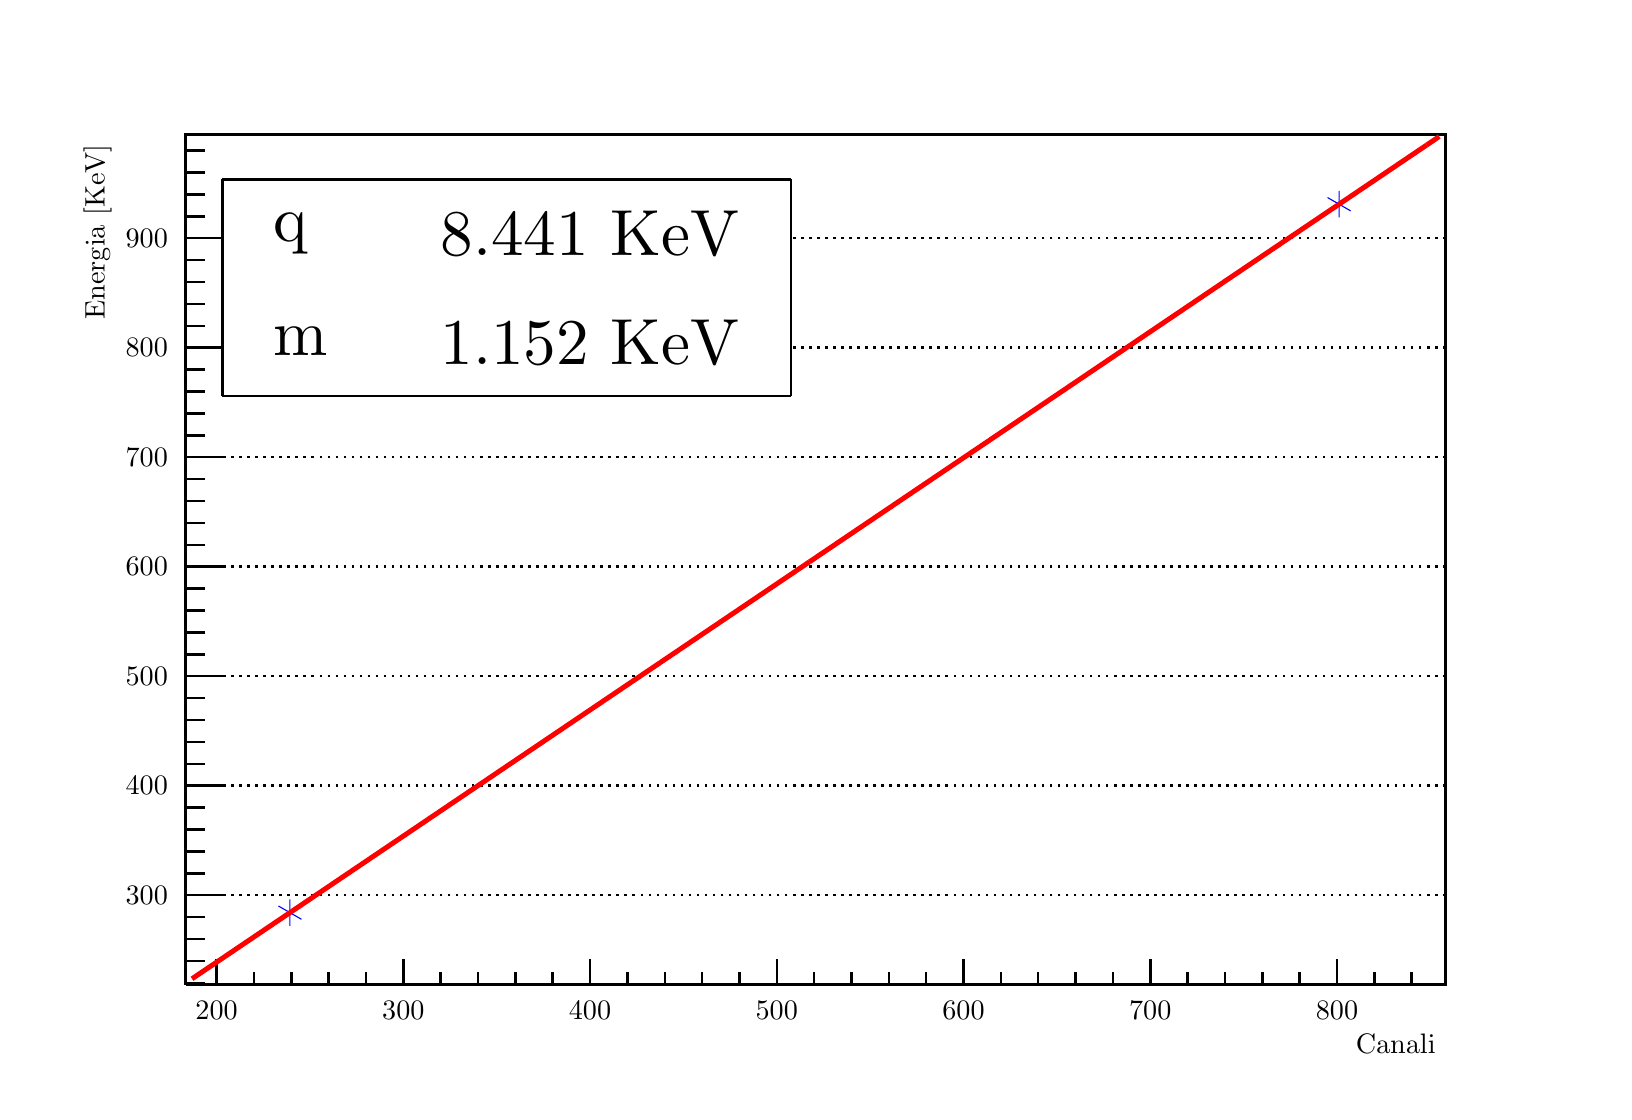
\begin{tikzpicture}
\pgfdeclareplotmark{cross} {
\pgfpathmoveto{\pgfpoint{-0.3\pgfplotmarksize}{\pgfplotmarksize}}
\pgfpathlineto{\pgfpoint{+0.3\pgfplotmarksize}{\pgfplotmarksize}}
\pgfpathlineto{\pgfpoint{+0.3\pgfplotmarksize}{0.3\pgfplotmarksize}}
\pgfpathlineto{\pgfpoint{+1\pgfplotmarksize}{0.3\pgfplotmarksize}}
\pgfpathlineto{\pgfpoint{+1\pgfplotmarksize}{-0.3\pgfplotmarksize}}
\pgfpathlineto{\pgfpoint{+0.3\pgfplotmarksize}{-0.3\pgfplotmarksize}}
\pgfpathlineto{\pgfpoint{+0.3\pgfplotmarksize}{-1.\pgfplotmarksize}}
\pgfpathlineto{\pgfpoint{-0.3\pgfplotmarksize}{-1.\pgfplotmarksize}}
\pgfpathlineto{\pgfpoint{-0.3\pgfplotmarksize}{-0.3\pgfplotmarksize}}
\pgfpathlineto{\pgfpoint{-1.\pgfplotmarksize}{-0.3\pgfplotmarksize}}
\pgfpathlineto{\pgfpoint{-1.\pgfplotmarksize}{0.3\pgfplotmarksize}}
\pgfpathlineto{\pgfpoint{-0.3\pgfplotmarksize}{0.3\pgfplotmarksize}}
\pgfpathclose
\pgfusepathqstroke
}
\pgfdeclareplotmark{cross*} {
\pgfpathmoveto{\pgfpoint{-0.3\pgfplotmarksize}{\pgfplotmarksize}}
\pgfpathlineto{\pgfpoint{+0.3\pgfplotmarksize}{\pgfplotmarksize}}
\pgfpathlineto{\pgfpoint{+0.3\pgfplotmarksize}{0.3\pgfplotmarksize}}
\pgfpathlineto{\pgfpoint{+1\pgfplotmarksize}{0.3\pgfplotmarksize}}
\pgfpathlineto{\pgfpoint{+1\pgfplotmarksize}{-0.3\pgfplotmarksize}}
\pgfpathlineto{\pgfpoint{+0.3\pgfplotmarksize}{-0.3\pgfplotmarksize}}
\pgfpathlineto{\pgfpoint{+0.3\pgfplotmarksize}{-1.\pgfplotmarksize}}
\pgfpathlineto{\pgfpoint{-0.3\pgfplotmarksize}{-1.\pgfplotmarksize}}
\pgfpathlineto{\pgfpoint{-0.3\pgfplotmarksize}{-0.3\pgfplotmarksize}}
\pgfpathlineto{\pgfpoint{-1.\pgfplotmarksize}{-0.3\pgfplotmarksize}}
\pgfpathlineto{\pgfpoint{-1.\pgfplotmarksize}{0.3\pgfplotmarksize}}
\pgfpathlineto{\pgfpoint{-0.3\pgfplotmarksize}{0.3\pgfplotmarksize}}
\pgfpathclose
\pgfusepathqfillstroke
}
\pgfdeclareplotmark{newstar} {
\pgfpathmoveto{\pgfqpoint{0pt}{\pgfplotmarksize}}
\pgfpathlineto{\pgfqpointpolar{44}{0.5\pgfplotmarksize}}
\pgfpathlineto{\pgfqpointpolar{18}{\pgfplotmarksize}}
\pgfpathlineto{\pgfqpointpolar{-20}{0.5\pgfplotmarksize}}
\pgfpathlineto{\pgfqpointpolar{-54}{\pgfplotmarksize}}
\pgfpathlineto{\pgfqpointpolar{-90}{0.5\pgfplotmarksize}}
\pgfpathlineto{\pgfqpointpolar{234}{\pgfplotmarksize}}
\pgfpathlineto{\pgfqpointpolar{198}{0.5\pgfplotmarksize}}
\pgfpathlineto{\pgfqpointpolar{162}{\pgfplotmarksize}}
\pgfpathlineto{\pgfqpointpolar{134}{0.5\pgfplotmarksize}}
\pgfpathclose
\pgfusepathqstroke
}
\pgfdeclareplotmark{newstar*} {
\pgfpathmoveto{\pgfqpoint{0pt}{\pgfplotmarksize}}
\pgfpathlineto{\pgfqpointpolar{44}{0.5\pgfplotmarksize}}
\pgfpathlineto{\pgfqpointpolar{18}{\pgfplotmarksize}}
\pgfpathlineto{\pgfqpointpolar{-20}{0.5\pgfplotmarksize}}
\pgfpathlineto{\pgfqpointpolar{-54}{\pgfplotmarksize}}
\pgfpathlineto{\pgfqpointpolar{-90}{0.5\pgfplotmarksize}}
\pgfpathlineto{\pgfqpointpolar{234}{\pgfplotmarksize}}
\pgfpathlineto{\pgfqpointpolar{198}{0.5\pgfplotmarksize}}
\pgfpathlineto{\pgfqpointpolar{162}{\pgfplotmarksize}}
\pgfpathlineto{\pgfqpointpolar{134}{0.5\pgfplotmarksize}}
\pgfpathclose
\pgfusepathqfillstroke
}
\definecolor{c}{rgb}{1,1,1};
\draw [color=c, fill=c] (0,0) rectangle (20,13.4957);
\draw [color=c, fill=c] (2,1.34957) rectangle (18,12.1461);
\definecolor{c}{rgb}{0,0,0};
\draw [c,line width=0.9] (2,1.34957) -- (2,12.1461) -- (18,12.1461) -- (18,1.34957) -- (2,1.34957);
\definecolor{c}{rgb}{1,1,1};
\draw [color=c, fill=c] (2,1.34957) rectangle (18,12.1461);
\definecolor{c}{rgb}{0,0,0};
\draw [c,line width=0.9] (2,1.34957) -- (2,12.1461) -- (18,12.1461) -- (18,1.34957) -- (2,1.34957);
\draw [c,line width=0.9] (2,1.34957) -- (18,1.34957);
\draw [c,line width=0.9] (2,1.34957) -- (2,12.1461);
\draw [c,dotted,line width=0.9] (18,2.48568) -- (2,2.48568);
\draw [c,dotted,line width=0.9] (18,3.87628) -- (2,3.87628);
\draw [c,dotted,line width=0.9] (18,5.26687) -- (2,5.26687);
\draw [c,dotted,line width=0.9] (18,6.65746) -- (2,6.65746);
\draw [c,dotted,line width=0.9] (18,8.04805) -- (2,8.04805);
\draw [c,dotted,line width=0.9] (18,9.43865) -- (2,9.43865);
\draw [c,dotted,line width=0.9] (18,10.8292) -- (2,10.8292);
\draw [c,dotted,line width=0.9] (18,2.48568) -- (2,2.48568);
\draw [c,dotted,line width=0.9] (18,10.8292) -- (2,10.8292);
\draw [c,line width=0.9] (2,1.34957) -- (18,1.34957);
\draw [anchor= east] (18,0.593811) node[scale=1.01821, color=c, rotate=0]{Canali};
\draw [c,line width=0.9] (2.39179,1.67347) -- (2.39179,1.34957);
\draw [c,line width=0.9] (2.86612,1.51152) -- (2.86612,1.34957);
\draw [c,line width=0.9] (3.34045,1.51152) -- (3.34045,1.34957);
\draw [c,line width=0.9] (3.81478,1.51152) -- (3.81478,1.34957);
\draw [c,line width=0.9] (4.2891,1.51152) -- (4.2891,1.34957);
\draw [c,line width=0.9] (4.76343,1.67347) -- (4.76343,1.34957);
\draw [c,line width=0.9] (5.23776,1.51152) -- (5.23776,1.34957);
\draw [c,line width=0.9] (5.71208,1.51152) -- (5.71208,1.34957);
\draw [c,line width=0.9] (6.18641,1.51152) -- (6.18641,1.34957);
\draw [c,line width=0.9] (6.66074,1.51152) -- (6.66074,1.34957);
\draw [c,line width=0.9] (7.13506,1.67347) -- (7.13506,1.34957);
\draw [c,line width=0.9] (7.60939,1.51152) -- (7.60939,1.34957);
\draw [c,line width=0.9] (8.08372,1.51152) -- (8.08372,1.34957);
\draw [c,line width=0.9] (8.55805,1.51152) -- (8.55805,1.34957);
\draw [c,line width=0.9] (9.03237,1.51152) -- (9.03237,1.34957);
\draw [c,line width=0.9] (9.5067,1.67347) -- (9.5067,1.34957);
\draw [c,line width=0.9] (9.98103,1.51152) -- (9.98103,1.34957);
\draw [c,line width=0.9] (10.4554,1.51152) -- (10.4554,1.34957);
\draw [c,line width=0.9] (10.9297,1.51152) -- (10.9297,1.34957);
\draw [c,line width=0.9] (11.404,1.51152) -- (11.404,1.34957);
\draw [c,line width=0.9] (11.8783,1.67347) -- (11.8783,1.34957);
\draw [c,line width=0.9] (12.3527,1.51152) -- (12.3527,1.34957);
\draw [c,line width=0.9] (12.827,1.51152) -- (12.827,1.34957);
\draw [c,line width=0.9] (13.3013,1.51152) -- (13.3013,1.34957);
\draw [c,line width=0.9] (13.7756,1.51152) -- (13.7756,1.34957);
\draw [c,line width=0.9] (14.25,1.67347) -- (14.25,1.34957);
\draw [c,line width=0.9] (14.7243,1.51152) -- (14.7243,1.34957);
\draw [c,line width=0.9] (15.1986,1.51152) -- (15.1986,1.34957);
\draw [c,line width=0.9] (15.673,1.51152) -- (15.673,1.34957);
\draw [c,line width=0.9] (16.1473,1.51152) -- (16.1473,1.34957);
\draw [c,line width=0.9] (16.6216,1.67347) -- (16.6216,1.34957);
\draw [c,line width=0.9] (2.39179,1.67347) -- (2.39179,1.34957);
\draw [c,line width=0.9] (16.6216,1.67347) -- (16.6216,1.34957);
\draw [c,line width=0.9] (17.0959,1.51152) -- (17.0959,1.34957);
\draw [c,line width=0.9] (17.5703,1.51152) -- (17.5703,1.34957);
\draw [anchor=base] (2.39179,0.904212) node[scale=1.01821, color=c, rotate=0]{200};
\draw [anchor=base] (4.76343,0.904212) node[scale=1.01821, color=c, rotate=0]{300};
\draw [anchor=base] (7.13506,0.904212) node[scale=1.01821, color=c, rotate=0]{400};
\draw [anchor=base] (9.5067,0.904212) node[scale=1.01821, color=c, rotate=0]{500};
\draw [anchor=base] (11.8783,0.904212) node[scale=1.01821, color=c, rotate=0]{600};
\draw [anchor=base] (14.25,0.904212) node[scale=1.01821, color=c, rotate=0]{700};
\draw [anchor=base] (16.6216,0.904212) node[scale=1.01821, color=c, rotate=0]{800};
\draw [c,line width=0.9] (2,1.34957) -- (2,12.1461);
\draw [anchor= east] (0.88,12.1461) node[scale=1.01821, color=c, rotate=90]{Energia [KeV]};
\draw [c,line width=0.9] (2.48,2.48568) -- (2,2.48568);
\draw [c,line width=0.9] (2.24,2.7638) -- (2,2.7638);
\draw [c,line width=0.9] (2.24,3.04192) -- (2,3.04192);
\draw [c,line width=0.9] (2.24,3.32004) -- (2,3.32004);
\draw [c,line width=0.9] (2.24,3.59816) -- (2,3.59816);
\draw [c,line width=0.9] (2.48,3.87628) -- (2,3.87628);
\draw [c,line width=0.9] (2.24,4.1544) -- (2,4.1544);
\draw [c,line width=0.9] (2.24,4.43251) -- (2,4.43251);
\draw [c,line width=0.9] (2.24,4.71063) -- (2,4.71063);
\draw [c,line width=0.9] (2.24,4.98875) -- (2,4.98875);
\draw [c,line width=0.9] (2.48,5.26687) -- (2,5.26687);
\draw [c,line width=0.9] (2.24,5.54499) -- (2,5.54499);
\draw [c,line width=0.9] (2.24,5.82311) -- (2,5.82311);
\draw [c,line width=0.9] (2.24,6.10123) -- (2,6.10123);
\draw [c,line width=0.9] (2.24,6.37934) -- (2,6.37934);
\draw [c,line width=0.9] (2.48,6.65746) -- (2,6.65746);
\draw [c,line width=0.9] (2.24,6.93558) -- (2,6.93558);
\draw [c,line width=0.9] (2.24,7.2137) -- (2,7.2137);
\draw [c,line width=0.9] (2.24,7.49182) -- (2,7.49182);
\draw [c,line width=0.9] (2.24,7.76994) -- (2,7.76994);
\draw [c,line width=0.9] (2.48,8.04805) -- (2,8.04805);
\draw [c,line width=0.9] (2.24,8.32617) -- (2,8.32617);
\draw [c,line width=0.9] (2.24,8.60429) -- (2,8.60429);
\draw [c,line width=0.9] (2.24,8.88241) -- (2,8.88241);
\draw [c,line width=0.9] (2.24,9.16053) -- (2,9.16053);
\draw [c,line width=0.9] (2.48,9.43865) -- (2,9.43865);
\draw [c,line width=0.9] (2.24,9.71677) -- (2,9.71677);
\draw [c,line width=0.9] (2.24,9.99488) -- (2,9.99488);
\draw [c,line width=0.9] (2.24,10.273) -- (2,10.273);
\draw [c,line width=0.9] (2.24,10.5511) -- (2,10.5511);
\draw [c,line width=0.9] (2.48,10.8292) -- (2,10.8292);
\draw [c,line width=0.9] (2.48,2.48568) -- (2,2.48568);
\draw [c,line width=0.9] (2.24,2.20757) -- (2,2.20757);
\draw [c,line width=0.9] (2.24,1.92945) -- (2,1.92945);
\draw [c,line width=0.9] (2.24,1.65133) -- (2,1.65133);
\draw [c,line width=0.9] (2.24,1.37321) -- (2,1.37321);
\draw [c,line width=0.9] (2.48,10.8292) -- (2,10.8292);
\draw [c,line width=0.9] (2.24,11.1074) -- (2,11.1074);
\draw [c,line width=0.9] (2.24,11.3855) -- (2,11.3855);
\draw [c,line width=0.9] (2.24,11.6636) -- (2,11.6636);
\draw [c,line width=0.9] (2.24,11.9417) -- (2,11.9417);
\draw [anchor= east] (1.9,2.48568) node[scale=1.01821, color=c, rotate=0]{300};
\draw [anchor= east] (1.9,3.87628) node[scale=1.01821, color=c, rotate=0]{400};
\draw [anchor= east] (1.9,5.26687) node[scale=1.01821, color=c, rotate=0]{500};
\draw [anchor= east] (1.9,6.65746) node[scale=1.01821, color=c, rotate=0]{600};
\draw [anchor= east] (1.9,8.04805) node[scale=1.01821, color=c, rotate=0]{700};
\draw [anchor= east] (1.9,9.43865) node[scale=1.01821, color=c, rotate=0]{800};
\draw [anchor= east] (1.9,10.8292) node[scale=1.01821, color=c, rotate=0]{900};
\definecolor{c}{rgb}{1,1,1};
\draw [color=c, fill=c] (2.46418,8.82521) rectangle (9.68481,11.5759);
\definecolor{c}{rgb}{0,0,0};
\draw [c,line width=0.9] (2.46418,8.82521) -- (9.68481,8.82521);
\draw [c,line width=0.9] (9.68481,8.82521) -- (9.68481,11.5759);
\draw [c,line width=0.9] (9.68481,11.5759) -- (2.46418,11.5759);
\draw [c,line width=0.9] (2.46418,11.5759) -- (2.46418,8.82521);
\draw [anchor= west] (2.82521,10.8883) node[scale=1.3364, color=c, rotate=0]{q       };
\draw [anchor= east] (9.32378,10.8883) node[scale=1.3364, color=c, rotate=0]{$ 8.441$ KeV};
\draw [anchor= west] (2.82521,9.51289) node[scale=1.3364, color=c, rotate=0]{m       };
\draw [anchor= east] (9.32378,9.51289) node[scale=1.3364, color=c, rotate=0]{$ 1.152$ KeV};
\definecolor{c}{rgb}{0,0,1};
\foreach \P in {(3.32378,2.26361),(16.6476,11.2607)}{\draw[mark options={color=c,fill=c},mark size=4.804805pt,mark=asterisk] plot coordinates {\P};}
\definecolor{c}{rgb}{1,0,0};
\draw [c,line width=1.8] (2.08,1.42372) -- (2.24,1.53177) -- (2.4,1.63981) -- (2.56,1.74785) -- (2.72,1.8559) -- (2.88,1.96394) -- (3.04,2.07198) -- (3.2,2.18002) -- (3.36,2.28807) -- (3.52,2.39611) -- (3.68,2.50415) -- (3.84,2.6122) -- (4,2.72024)
 -- (4.16,2.82828) -- (4.32,2.93633) -- (4.48,3.04437) -- (4.64,3.15241) -- (4.8,3.26045) -- (4.96,3.3685) -- (5.12,3.47654) -- (5.28,3.58458) -- (5.44,3.69263) -- (5.6,3.80067) -- (5.76,3.90871) -- (5.92,4.01676) -- (6.08,4.1248) -- (6.24,4.23284)
 -- (6.4,4.34088) -- (6.56,4.44893) -- (6.72,4.55697) -- (6.88,4.66501) -- (7.04,4.77306) -- (7.2,4.8811) -- (7.36,4.98914) -- (7.52,5.09719) -- (7.68,5.20523) -- (7.84,5.31327) -- (8,5.42131) -- (8.16,5.52936) -- (8.32,5.6374) -- (8.48,5.74544) --
 (8.64,5.85349) -- (8.8,5.96153) -- (8.96,6.06957) -- (9.12,6.17762) -- (9.28,6.28566) -- (9.44,6.3937) -- (9.6,6.50174) -- (9.76,6.60979) -- (9.92,6.71783);
\draw [c,line width=1.8] (9.92,6.71783) -- (10.08,6.82587) -- (10.24,6.93392) -- (10.4,7.04196) -- (10.56,7.15) -- (10.72,7.25805) -- (10.88,7.36609) -- (11.04,7.47413) -- (11.2,7.58217) -- (11.36,7.69022) -- (11.52,7.79826) -- (11.68,7.9063) --
 (11.84,8.01435) -- (12,8.12239) -- (12.16,8.23043) -- (12.32,8.33848) -- (12.48,8.44652) -- (12.64,8.55456) -- (12.8,8.6626) -- (12.96,8.77065) -- (13.12,8.87869) -- (13.28,8.98673) -- (13.44,9.09478) -- (13.6,9.20282) -- (13.76,9.31086) --
 (13.92,9.41891) -- (14.08,9.52695) -- (14.24,9.63499) -- (14.4,9.74303) -- (14.56,9.85108) -- (14.72,9.95912) -- (14.88,10.0672) -- (15.04,10.1752) -- (15.2,10.2832) -- (15.36,10.3913) -- (15.52,10.4993) -- (15.68,10.6074) -- (15.84,10.7154) --
 (16,10.8235) -- (16.16,10.9315) -- (16.32,11.0396) -- (16.48,11.1476) -- (16.64,11.2556) -- (16.8,11.3637) -- (16.96,11.4717) -- (17.12,11.5798) -- (17.28,11.6878) -- (17.44,11.7959) -- (17.6,11.9039) -- (17.76,12.0119);
\draw [c,line width=1.8] (17.76,12.0119) -- (17.92,12.12);
\definecolor{c}{rgb}{1,1,1};
\draw [color=c, fill=c] (2.46418,8.82521) rectangle (9.68481,11.5759);
\definecolor{c}{rgb}{0,0,0};
\draw [c,line width=0.9] (2.46418,8.82521) -- (9.68481,8.82521);
\draw [c,line width=0.9] (9.68481,8.82521) -- (9.68481,11.5759);
\draw [c,line width=0.9] (9.68481,11.5759) -- (2.46418,11.5759);
\draw [c,line width=0.9] (2.46418,11.5759) -- (2.46418,8.82521);
\draw [anchor= west] (2.82521,10.8883) node[scale=2.35461, color=c, rotate=0]{q       };
\draw [anchor= east] (9.32378,10.8883) node[scale=2.35461, color=c, rotate=0]{$ 8.441$ KeV};
\draw [anchor= west] (2.82521,9.51289) node[scale=2.35461, color=c, rotate=0]{m       };
\draw [anchor= east] (9.32378,9.51289) node[scale=2.35461, color=c, rotate=0]{$ 1.152$ KeV};
%\draw (10,12.808) node[scale=1.40004, color=c, rotate=0]{Calibrazione Energia Rivelatore 1};
\end{tikzpicture}

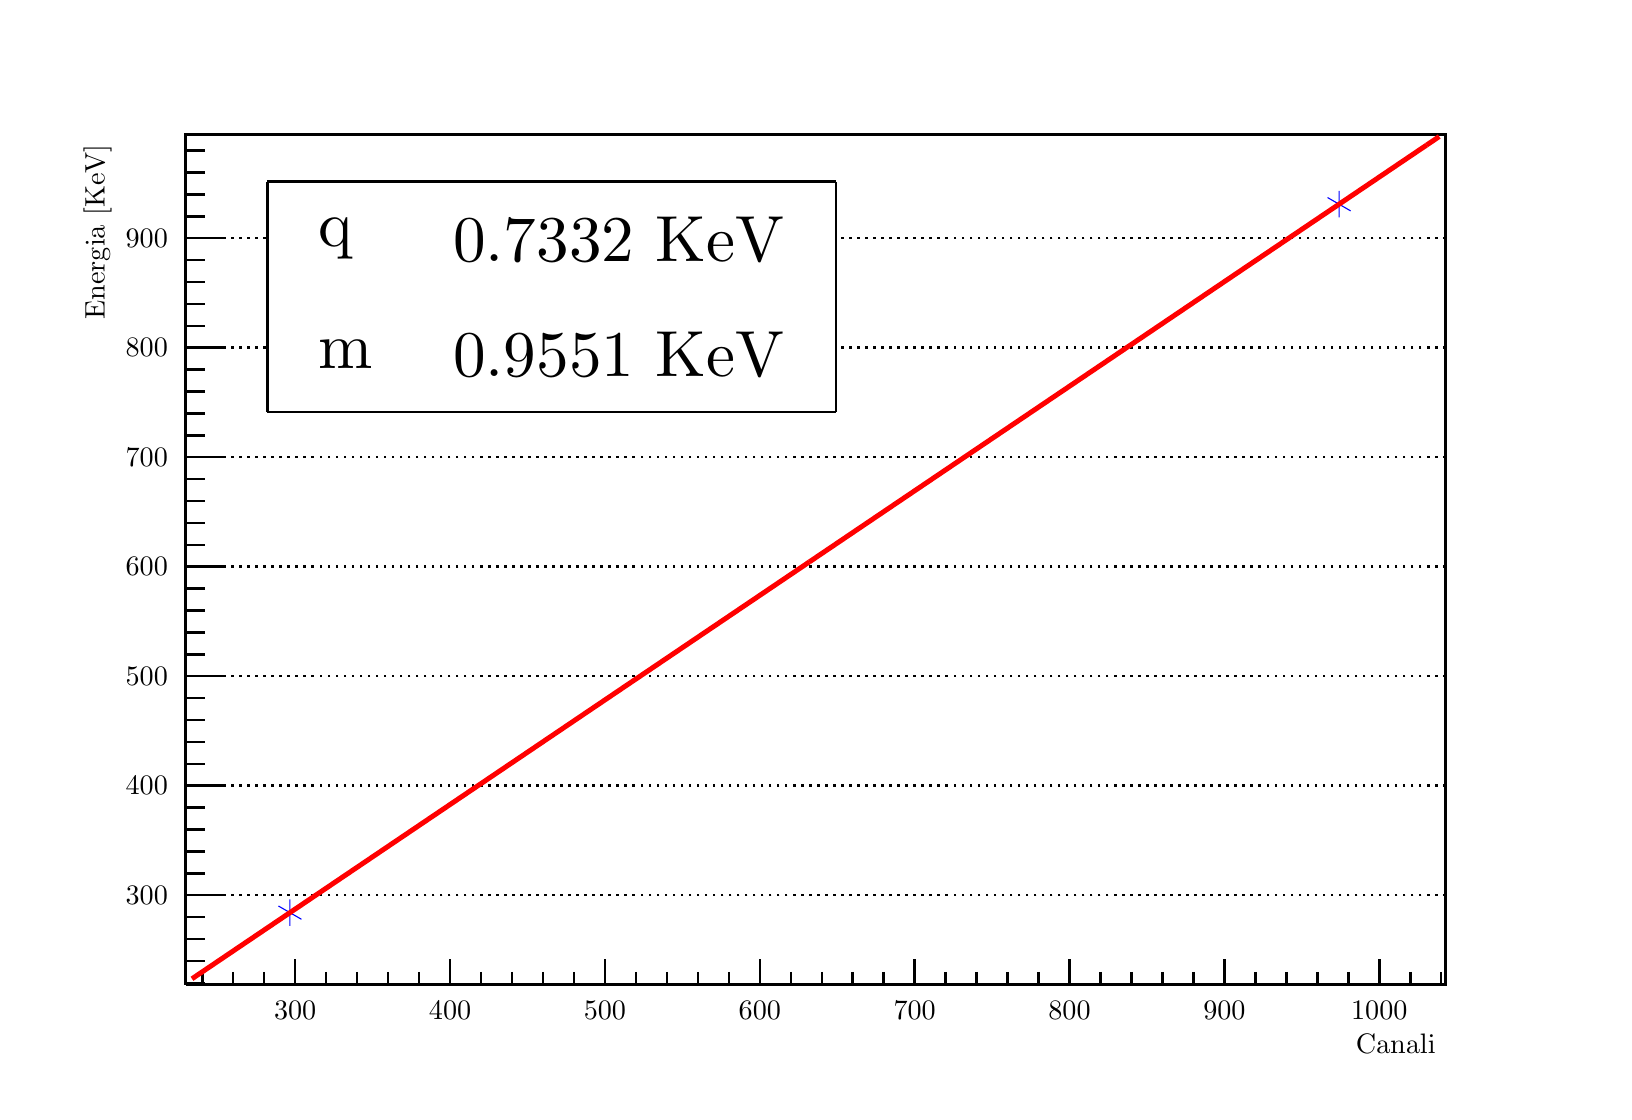
\begin{tikzpicture}
\pgfdeclareplotmark{cross} {
\pgfpathmoveto{\pgfpoint{-0.3\pgfplotmarksize}{\pgfplotmarksize}}
\pgfpathlineto{\pgfpoint{+0.3\pgfplotmarksize}{\pgfplotmarksize}}
\pgfpathlineto{\pgfpoint{+0.3\pgfplotmarksize}{0.3\pgfplotmarksize}}
\pgfpathlineto{\pgfpoint{+1\pgfplotmarksize}{0.3\pgfplotmarksize}}
\pgfpathlineto{\pgfpoint{+1\pgfplotmarksize}{-0.3\pgfplotmarksize}}
\pgfpathlineto{\pgfpoint{+0.3\pgfplotmarksize}{-0.3\pgfplotmarksize}}
\pgfpathlineto{\pgfpoint{+0.3\pgfplotmarksize}{-1.\pgfplotmarksize}}
\pgfpathlineto{\pgfpoint{-0.3\pgfplotmarksize}{-1.\pgfplotmarksize}}
\pgfpathlineto{\pgfpoint{-0.3\pgfplotmarksize}{-0.3\pgfplotmarksize}}
\pgfpathlineto{\pgfpoint{-1.\pgfplotmarksize}{-0.3\pgfplotmarksize}}
\pgfpathlineto{\pgfpoint{-1.\pgfplotmarksize}{0.3\pgfplotmarksize}}
\pgfpathlineto{\pgfpoint{-0.3\pgfplotmarksize}{0.3\pgfplotmarksize}}
\pgfpathclose
\pgfusepathqstroke
}
\pgfdeclareplotmark{cross*} {
\pgfpathmoveto{\pgfpoint{-0.3\pgfplotmarksize}{\pgfplotmarksize}}
\pgfpathlineto{\pgfpoint{+0.3\pgfplotmarksize}{\pgfplotmarksize}}
\pgfpathlineto{\pgfpoint{+0.3\pgfplotmarksize}{0.3\pgfplotmarksize}}
\pgfpathlineto{\pgfpoint{+1\pgfplotmarksize}{0.3\pgfplotmarksize}}
\pgfpathlineto{\pgfpoint{+1\pgfplotmarksize}{-0.3\pgfplotmarksize}}
\pgfpathlineto{\pgfpoint{+0.3\pgfplotmarksize}{-0.3\pgfplotmarksize}}
\pgfpathlineto{\pgfpoint{+0.3\pgfplotmarksize}{-1.\pgfplotmarksize}}
\pgfpathlineto{\pgfpoint{-0.3\pgfplotmarksize}{-1.\pgfplotmarksize}}
\pgfpathlineto{\pgfpoint{-0.3\pgfplotmarksize}{-0.3\pgfplotmarksize}}
\pgfpathlineto{\pgfpoint{-1.\pgfplotmarksize}{-0.3\pgfplotmarksize}}
\pgfpathlineto{\pgfpoint{-1.\pgfplotmarksize}{0.3\pgfplotmarksize}}
\pgfpathlineto{\pgfpoint{-0.3\pgfplotmarksize}{0.3\pgfplotmarksize}}
\pgfpathclose
\pgfusepathqfillstroke
}
\pgfdeclareplotmark{newstar} {
\pgfpathmoveto{\pgfqpoint{0pt}{\pgfplotmarksize}}
\pgfpathlineto{\pgfqpointpolar{44}{0.5\pgfplotmarksize}}
\pgfpathlineto{\pgfqpointpolar{18}{\pgfplotmarksize}}
\pgfpathlineto{\pgfqpointpolar{-20}{0.5\pgfplotmarksize}}
\pgfpathlineto{\pgfqpointpolar{-54}{\pgfplotmarksize}}
\pgfpathlineto{\pgfqpointpolar{-90}{0.5\pgfplotmarksize}}
\pgfpathlineto{\pgfqpointpolar{234}{\pgfplotmarksize}}
\pgfpathlineto{\pgfqpointpolar{198}{0.5\pgfplotmarksize}}
\pgfpathlineto{\pgfqpointpolar{162}{\pgfplotmarksize}}
\pgfpathlineto{\pgfqpointpolar{134}{0.5\pgfplotmarksize}}
\pgfpathclose
\pgfusepathqstroke
}
\pgfdeclareplotmark{newstar*} {
\pgfpathmoveto{\pgfqpoint{0pt}{\pgfplotmarksize}}
\pgfpathlineto{\pgfqpointpolar{44}{0.5\pgfplotmarksize}}
\pgfpathlineto{\pgfqpointpolar{18}{\pgfplotmarksize}}
\pgfpathlineto{\pgfqpointpolar{-20}{0.5\pgfplotmarksize}}
\pgfpathlineto{\pgfqpointpolar{-54}{\pgfplotmarksize}}
\pgfpathlineto{\pgfqpointpolar{-90}{0.5\pgfplotmarksize}}
\pgfpathlineto{\pgfqpointpolar{234}{\pgfplotmarksize}}
\pgfpathlineto{\pgfqpointpolar{198}{0.5\pgfplotmarksize}}
\pgfpathlineto{\pgfqpointpolar{162}{\pgfplotmarksize}}
\pgfpathlineto{\pgfqpointpolar{134}{0.5\pgfplotmarksize}}
\pgfpathclose
\pgfusepathqfillstroke
}
\definecolor{c}{rgb}{1,1,1};
\draw [color=c, fill=c] (0,0) rectangle (20,13.4957);
\draw [color=c, fill=c] (2,1.34957) rectangle (18,12.1461);
\definecolor{c}{rgb}{0,0,0};
\draw [c,line width=0.9] (2,1.34957) -- (2,12.1461) -- (18,12.1461) -- (18,1.34957) -- (2,1.34957);
\definecolor{c}{rgb}{1,1,1};
\draw [color=c, fill=c] (2,1.34957) rectangle (18,12.1461);
\definecolor{c}{rgb}{0,0,0};
\draw [c,line width=0.9] (2,1.34957) -- (2,12.1461) -- (18,12.1461) -- (18,1.34957) -- (2,1.34957);
\draw [c,line width=0.9] (2,1.34957) -- (18,1.34957);
\draw [c,line width=0.9] (2,1.34957) -- (2,12.1461);
\draw [c,dotted,line width=0.9] (18,2.48568) -- (2,2.48568);
\draw [c,dotted,line width=0.9] (18,3.87628) -- (2,3.87628);
\draw [c,dotted,line width=0.9] (18,5.26687) -- (2,5.26687);
\draw [c,dotted,line width=0.9] (18,6.65746) -- (2,6.65746);
\draw [c,dotted,line width=0.9] (18,8.04805) -- (2,8.04805);
\draw [c,dotted,line width=0.9] (18,9.43865) -- (2,9.43865);
\draw [c,dotted,line width=0.9] (18,10.8292) -- (2,10.8292);
\draw [c,dotted,line width=0.9] (18,2.48568) -- (2,2.48568);
\draw [c,dotted,line width=0.9] (18,10.8292) -- (2,10.8292);
\draw [c,line width=0.9] (2,1.34957) -- (18,1.34957);
\draw [anchor= east] (18,0.593811) node[scale=1.01821, color=c, rotate=0]{Canali};
\draw [c,line width=0.9] (3.39037,1.67347) -- (3.39037,1.34957);
\draw [c,line width=0.9] (3.78374,1.51152) -- (3.78374,1.34957);
\draw [c,line width=0.9] (4.17712,1.51152) -- (4.17712,1.34957);
\draw [c,line width=0.9] (4.57049,1.51152) -- (4.57049,1.34957);
\draw [c,line width=0.9] (4.96386,1.51152) -- (4.96386,1.34957);
\draw [c,line width=0.9] (5.35723,1.67347) -- (5.35723,1.34957);
\draw [c,line width=0.9] (5.7506,1.51152) -- (5.7506,1.34957);
\draw [c,line width=0.9] (6.14397,1.51152) -- (6.14397,1.34957);
\draw [c,line width=0.9] (6.53735,1.51152) -- (6.53735,1.34957);
\draw [c,line width=0.9] (6.93072,1.51152) -- (6.93072,1.34957);
\draw [c,line width=0.9] (7.32409,1.67347) -- (7.32409,1.34957);
\draw [c,line width=0.9] (7.71746,1.51152) -- (7.71746,1.34957);
\draw [c,line width=0.9] (8.11083,1.51152) -- (8.11083,1.34957);
\draw [c,line width=0.9] (8.5042,1.51152) -- (8.5042,1.34957);
\draw [c,line width=0.9] (8.89758,1.51152) -- (8.89758,1.34957);
\draw [c,line width=0.9] (9.29095,1.67347) -- (9.29095,1.34957);
\draw [c,line width=0.9] (9.68432,1.51152) -- (9.68432,1.34957);
\draw [c,line width=0.9] (10.0777,1.51152) -- (10.0777,1.34957);
\draw [c,line width=0.9] (10.4711,1.51152) -- (10.4711,1.34957);
\draw [c,line width=0.9] (10.8644,1.51152) -- (10.8644,1.34957);
\draw [c,line width=0.9] (11.2578,1.67347) -- (11.2578,1.34957);
\draw [c,line width=0.9] (11.6512,1.51152) -- (11.6512,1.34957);
\draw [c,line width=0.9] (12.0445,1.51152) -- (12.0445,1.34957);
\draw [c,line width=0.9] (12.4379,1.51152) -- (12.4379,1.34957);
\draw [c,line width=0.9] (12.8313,1.51152) -- (12.8313,1.34957);
\draw [c,line width=0.9] (13.2247,1.67347) -- (13.2247,1.34957);
\draw [c,line width=0.9] (13.618,1.51152) -- (13.618,1.34957);
\draw [c,line width=0.9] (14.0114,1.51152) -- (14.0114,1.34957);
\draw [c,line width=0.9] (14.4048,1.51152) -- (14.4048,1.34957);
\draw [c,line width=0.9] (14.7982,1.51152) -- (14.7982,1.34957);
\draw [c,line width=0.9] (15.1915,1.67347) -- (15.1915,1.34957);
\draw [c,line width=0.9] (15.5849,1.51152) -- (15.5849,1.34957);
\draw [c,line width=0.9] (15.9783,1.51152) -- (15.9783,1.34957);
\draw [c,line width=0.9] (16.3716,1.51152) -- (16.3716,1.34957);
\draw [c,line width=0.9] (16.765,1.51152) -- (16.765,1.34957);
\draw [c,line width=0.9] (17.1584,1.67347) -- (17.1584,1.34957);
\draw [c,line width=0.9] (3.39037,1.67347) -- (3.39037,1.34957);
\draw [c,line width=0.9] (2.997,1.51152) -- (2.997,1.34957);
\draw [c,line width=0.9] (2.60363,1.51152) -- (2.60363,1.34957);
\draw [c,line width=0.9] (2.21026,1.51152) -- (2.21026,1.34957);
\draw [c,line width=0.9] (17.1584,1.67347) -- (17.1584,1.34957);
\draw [c,line width=0.9] (17.5518,1.51152) -- (17.5518,1.34957);
\draw [c,line width=0.9] (17.9451,1.51152) -- (17.9451,1.34957);
\draw [anchor=base] (3.39037,0.904212) node[scale=1.01821, color=c, rotate=0]{300};
\draw [anchor=base] (5.35723,0.904212) node[scale=1.01821, color=c, rotate=0]{400};
\draw [anchor=base] (7.32409,0.904212) node[scale=1.01821, color=c, rotate=0]{500};
\draw [anchor=base] (9.29095,0.904212) node[scale=1.01821, color=c, rotate=0]{600};
\draw [anchor=base] (11.2578,0.904212) node[scale=1.01821, color=c, rotate=0]{700};
\draw [anchor=base] (13.2247,0.904212) node[scale=1.01821, color=c, rotate=0]{800};
\draw [anchor=base] (15.1915,0.904212) node[scale=1.01821, color=c, rotate=0]{900};
\draw [anchor=base] (17.1584,0.904212) node[scale=1.01821, color=c, rotate=0]{1000};
\draw [c,line width=0.9] (2,1.34957) -- (2,12.1461);
\draw [anchor= east] (0.88,12.1461) node[scale=1.01821, color=c, rotate=90]{Energia [KeV]};
\draw [c,line width=0.9] (2.48,2.48568) -- (2,2.48568);
\draw [c,line width=0.9] (2.24,2.7638) -- (2,2.7638);
\draw [c,line width=0.9] (2.24,3.04192) -- (2,3.04192);
\draw [c,line width=0.9] (2.24,3.32004) -- (2,3.32004);
\draw [c,line width=0.9] (2.24,3.59816) -- (2,3.59816);
\draw [c,line width=0.9] (2.48,3.87628) -- (2,3.87628);
\draw [c,line width=0.9] (2.24,4.1544) -- (2,4.1544);
\draw [c,line width=0.9] (2.24,4.43251) -- (2,4.43251);
\draw [c,line width=0.9] (2.24,4.71063) -- (2,4.71063);
\draw [c,line width=0.9] (2.24,4.98875) -- (2,4.98875);
\draw [c,line width=0.9] (2.48,5.26687) -- (2,5.26687);
\draw [c,line width=0.9] (2.24,5.54499) -- (2,5.54499);
\draw [c,line width=0.9] (2.24,5.82311) -- (2,5.82311);
\draw [c,line width=0.9] (2.24,6.10123) -- (2,6.10123);
\draw [c,line width=0.9] (2.24,6.37934) -- (2,6.37934);
\draw [c,line width=0.9] (2.48,6.65746) -- (2,6.65746);
\draw [c,line width=0.9] (2.24,6.93558) -- (2,6.93558);
\draw [c,line width=0.9] (2.24,7.2137) -- (2,7.2137);
\draw [c,line width=0.9] (2.24,7.49182) -- (2,7.49182);
\draw [c,line width=0.9] (2.24,7.76994) -- (2,7.76994);
\draw [c,line width=0.9] (2.48,8.04805) -- (2,8.04805);
\draw [c,line width=0.9] (2.24,8.32617) -- (2,8.32617);
\draw [c,line width=0.9] (2.24,8.60429) -- (2,8.60429);
\draw [c,line width=0.9] (2.24,8.88241) -- (2,8.88241);
\draw [c,line width=0.9] (2.24,9.16053) -- (2,9.16053);
\draw [c,line width=0.9] (2.48,9.43865) -- (2,9.43865);
\draw [c,line width=0.9] (2.24,9.71677) -- (2,9.71677);
\draw [c,line width=0.9] (2.24,9.99488) -- (2,9.99488);
\draw [c,line width=0.9] (2.24,10.273) -- (2,10.273);
\draw [c,line width=0.9] (2.24,10.5511) -- (2,10.5511);
\draw [c,line width=0.9] (2.48,10.8292) -- (2,10.8292);
\draw [c,line width=0.9] (2.48,2.48568) -- (2,2.48568);
\draw [c,line width=0.9] (2.24,2.20757) -- (2,2.20757);
\draw [c,line width=0.9] (2.24,1.92945) -- (2,1.92945);
\draw [c,line width=0.9] (2.24,1.65133) -- (2,1.65133);
\draw [c,line width=0.9] (2.24,1.37321) -- (2,1.37321);
\draw [c,line width=0.9] (2.48,10.8292) -- (2,10.8292);
\draw [c,line width=0.9] (2.24,11.1074) -- (2,11.1074);
\draw [c,line width=0.9] (2.24,11.3855) -- (2,11.3855);
\draw [c,line width=0.9] (2.24,11.6636) -- (2,11.6636);
\draw [c,line width=0.9] (2.24,11.9417) -- (2,11.9417);
\draw [anchor= east] (1.9,2.48568) node[scale=1.01821, color=c, rotate=0]{300};
\draw [anchor= east] (1.9,3.87628) node[scale=1.01821, color=c, rotate=0]{400};
\draw [anchor= east] (1.9,5.26687) node[scale=1.01821, color=c, rotate=0]{500};
\draw [anchor= east] (1.9,6.65746) node[scale=1.01821, color=c, rotate=0]{600};
\draw [anchor= east] (1.9,8.04805) node[scale=1.01821, color=c, rotate=0]{700};
\draw [anchor= east] (1.9,9.43865) node[scale=1.01821, color=c, rotate=0]{800};
\draw [anchor= east] (1.9,10.8292) node[scale=1.01821, color=c, rotate=0]{900};
\definecolor{c}{rgb}{1,1,1};
\draw [color=c, fill=c] (3.03725,8.62464) rectangle (10.2579,11.5473);
\definecolor{c}{rgb}{0,0,0};
\draw [c,line width=0.9] (3.03725,8.62464) -- (10.2579,8.62464);
\draw [c,line width=0.9] (10.2579,8.62464) -- (10.2579,11.5473);
\draw [c,line width=0.9] (10.2579,11.5473) -- (3.03725,11.5473);
\draw [c,line width=0.9] (3.03725,11.5473) -- (3.03725,8.62464);
\draw [anchor= west] (3.39828,10.8166) node[scale=1.3364, color=c, rotate=0]{q       };
\draw [anchor= east] (9.89685,10.8166) node[scale=1.3364, color=c, rotate=0]{$ 0.7332$ KeV};
\draw [anchor= west] (3.39828,9.3553) node[scale=1.3364, color=c, rotate=0]{m       };
\draw [anchor= east] (9.89685,9.3553) node[scale=1.3364, color=c, rotate=0]{$ 0.9551$ KeV};
\definecolor{c}{rgb}{0,0,1};
\foreach \P in {(3.32378,2.26361),(16.6476,11.2607)}{\draw[mark options={color=c,fill=c},mark size=4.804805pt,mark=asterisk] plot coordinates {\P};}
\definecolor{c}{rgb}{1,0,0};
\draw [c,line width=1.8] (2.08,1.42372) -- (2.24,1.53177) -- (2.4,1.63981) -- (2.56,1.74785) -- (2.72,1.8559) -- (2.88,1.96394) -- (3.04,2.07198) -- (3.2,2.18002) -- (3.36,2.28807) -- (3.52,2.39611) -- (3.68,2.50415) -- (3.84,2.6122) -- (4,2.72024)
 -- (4.16,2.82828) -- (4.32,2.93633) -- (4.48,3.04437) -- (4.64,3.15241) -- (4.8,3.26045) -- (4.96,3.3685) -- (5.12,3.47654) -- (5.28,3.58458) -- (5.44,3.69263) -- (5.6,3.80067) -- (5.76,3.90871) -- (5.92,4.01676) -- (6.08,4.1248) -- (6.24,4.23284)
 -- (6.4,4.34088) -- (6.56,4.44893) -- (6.72,4.55697) -- (6.88,4.66501) -- (7.04,4.77306) -- (7.2,4.8811) -- (7.36,4.98914) -- (7.52,5.09719) -- (7.68,5.20523) -- (7.84,5.31327) -- (8,5.42131) -- (8.16,5.52936) -- (8.32,5.6374) -- (8.48,5.74544) --
 (8.64,5.85349) -- (8.8,5.96153) -- (8.96,6.06957) -- (9.12,6.17762) -- (9.28,6.28566) -- (9.44,6.3937) -- (9.6,6.50174) -- (9.76,6.60979) -- (9.92,6.71783);
\draw [c,line width=1.8] (9.92,6.71783) -- (10.08,6.82587) -- (10.24,6.93392) -- (10.4,7.04196) -- (10.56,7.15) -- (10.72,7.25805) -- (10.88,7.36609) -- (11.04,7.47413) -- (11.2,7.58217) -- (11.36,7.69022) -- (11.52,7.79826) -- (11.68,7.9063) --
 (11.84,8.01435) -- (12,8.12239) -- (12.16,8.23043) -- (12.32,8.33848) -- (12.48,8.44652) -- (12.64,8.55456) -- (12.8,8.6626) -- (12.96,8.77065) -- (13.12,8.87869) -- (13.28,8.98673) -- (13.44,9.09478) -- (13.6,9.20282) -- (13.76,9.31086) --
 (13.92,9.41891) -- (14.08,9.52695) -- (14.24,9.63499) -- (14.4,9.74303) -- (14.56,9.85108) -- (14.72,9.95912) -- (14.88,10.0672) -- (15.04,10.1752) -- (15.2,10.2832) -- (15.36,10.3913) -- (15.52,10.4993) -- (15.68,10.6074) -- (15.84,10.7154) --
 (16,10.8235) -- (16.16,10.9315) -- (16.32,11.0396) -- (16.48,11.1476) -- (16.64,11.2556) -- (16.8,11.3637) -- (16.96,11.4717) -- (17.12,11.5798) -- (17.28,11.6878) -- (17.44,11.7959) -- (17.6,11.9039) -- (17.76,12.0119);
\draw [c,line width=1.8] (17.76,12.0119) -- (17.92,12.12);
\definecolor{c}{rgb}{1,1,1};
\draw [color=c, fill=c] (3.03725,8.62464) rectangle (10.2579,11.5473);
\definecolor{c}{rgb}{0,0,0};
\draw [c,line width=0.9] (3.03725,8.62464) -- (10.2579,8.62464);
\draw [c,line width=0.9] (10.2579,8.62464) -- (10.2579,11.5473);
\draw [c,line width=0.9] (10.2579,11.5473) -- (3.03725,11.5473);
\draw [c,line width=0.9] (3.03725,11.5473) -- (3.03725,8.62464);
\draw [anchor= west] (3.39828,10.8166) node[scale=2.35461, color=c, rotate=0]{q       };
\draw [anchor= east] (9.89685,10.8166) node[scale=2.35461, color=c, rotate=0]{$ 0.7332$ KeV};
\draw [anchor= west] (3.39828,9.3553) node[scale=2.35461, color=c, rotate=0]{m       };
\draw [anchor= east] (9.89685,9.3553) node[scale=2.35461, color=c, rotate=0]{$ 0.9551$ KeV};
%\draw (10,12.808) node[scale=1.40004, color=c, rotate=0]{Calibrazione Energia Rivelatore 2};
\end{tikzpicture}


\section{Calibrazione in Tempo}

A questo punto si è proceduto con la calibrazione in tempo, acquisendo lo spettro del TAC (CH1 canale dell'MCA) avendo settato differenti ritardi tramite 
un'apposita cassetta dei ritardi. Interpolando tali spettri con una gaussiana si è potuto ottenere nuovamente centroide con relativo 
errore corrispondenti ai vari ritardi della delay unit (tra i 4 ns ed i 30 ns) ,
ed effettuando quindi un'interpolazione lineare. Nella seguente tabella si possono vedere i risultati dell'interpolazione gaussiana usati per la calibrazione. Si presenta qui per brevità solo un grafico contenente tutti gli spettri insieme privi di fit (Fig \ref{hist:calib_delay}). \footnote{i singoli grafici di interpolazione gaussiana possono essere visti in Appendice.}. \\

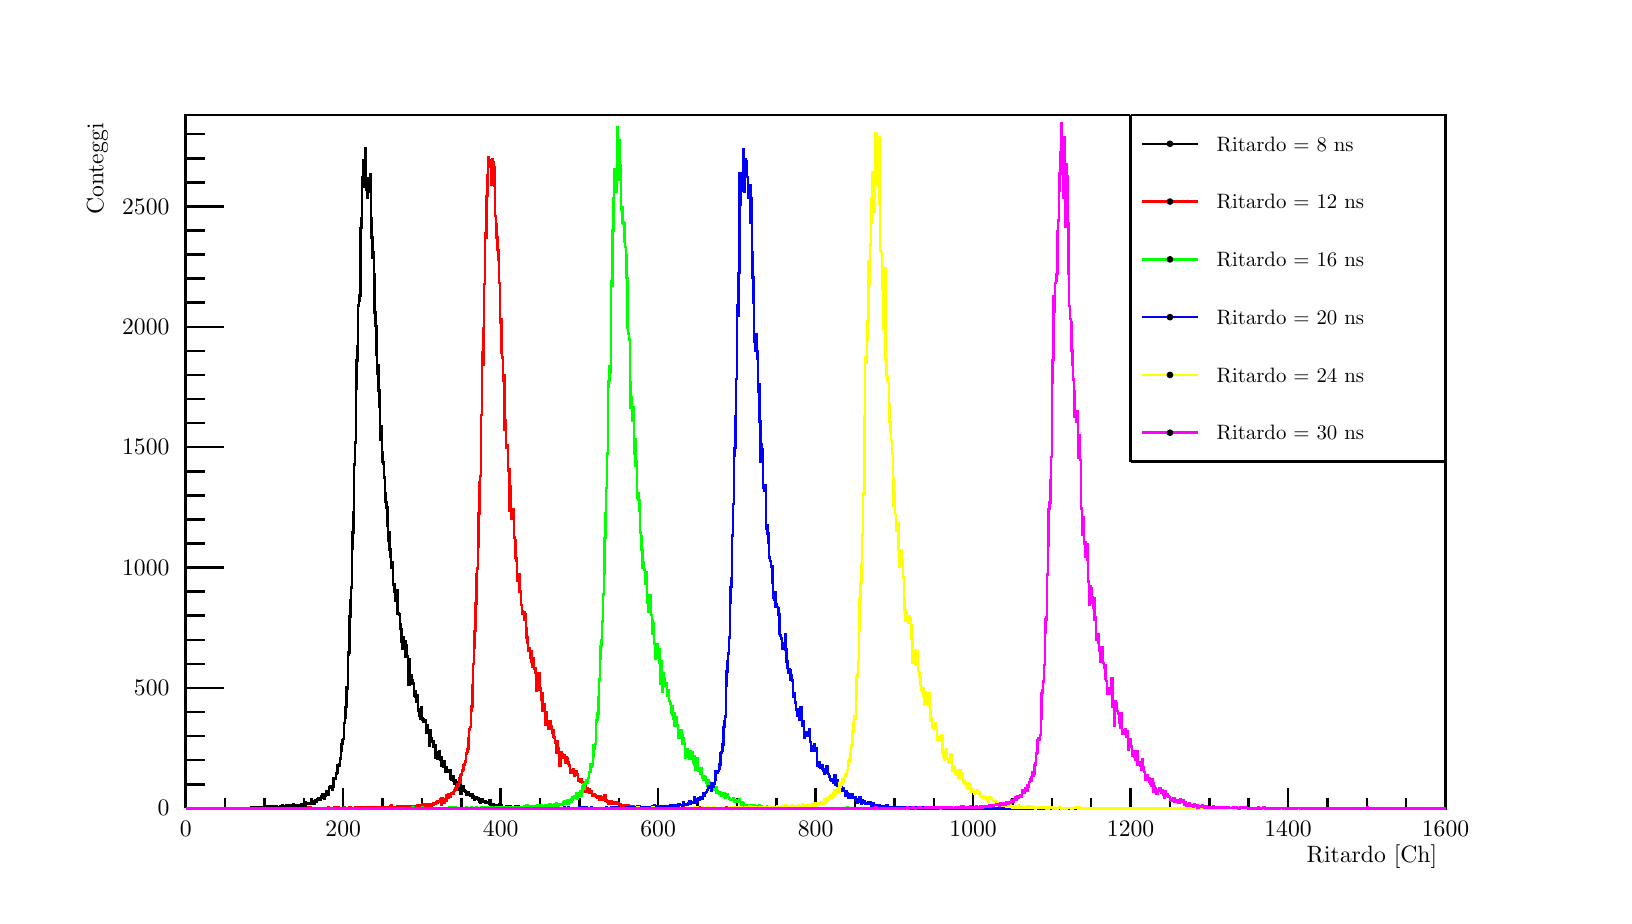
\begin{tikzpicture}
\pgfdeclareplotmark{cross} {
\pgfpathmoveto{\pgfpoint{-0.3\pgfplotmarksize}{\pgfplotmarksize}}
\pgfpathlineto{\pgfpoint{+0.3\pgfplotmarksize}{\pgfplotmarksize}}
\pgfpathlineto{\pgfpoint{+0.3\pgfplotmarksize}{0.3\pgfplotmarksize}}
\pgfpathlineto{\pgfpoint{+1\pgfplotmarksize}{0.3\pgfplotmarksize}}
\pgfpathlineto{\pgfpoint{+1\pgfplotmarksize}{-0.3\pgfplotmarksize}}
\pgfpathlineto{\pgfpoint{+0.3\pgfplotmarksize}{-0.3\pgfplotmarksize}}
\pgfpathlineto{\pgfpoint{+0.3\pgfplotmarksize}{-1.\pgfplotmarksize}}
\pgfpathlineto{\pgfpoint{-0.3\pgfplotmarksize}{-1.\pgfplotmarksize}}
\pgfpathlineto{\pgfpoint{-0.3\pgfplotmarksize}{-0.3\pgfplotmarksize}}
\pgfpathlineto{\pgfpoint{-1.\pgfplotmarksize}{-0.3\pgfplotmarksize}}
\pgfpathlineto{\pgfpoint{-1.\pgfplotmarksize}{0.3\pgfplotmarksize}}
\pgfpathlineto{\pgfpoint{-0.3\pgfplotmarksize}{0.3\pgfplotmarksize}}
\pgfpathclose
\pgfusepathqstroke
}
\pgfdeclareplotmark{cross*} {
\pgfpathmoveto{\pgfpoint{-0.3\pgfplotmarksize}{\pgfplotmarksize}}
\pgfpathlineto{\pgfpoint{+0.3\pgfplotmarksize}{\pgfplotmarksize}}
\pgfpathlineto{\pgfpoint{+0.3\pgfplotmarksize}{0.3\pgfplotmarksize}}
\pgfpathlineto{\pgfpoint{+1\pgfplotmarksize}{0.3\pgfplotmarksize}}
\pgfpathlineto{\pgfpoint{+1\pgfplotmarksize}{-0.3\pgfplotmarksize}}
\pgfpathlineto{\pgfpoint{+0.3\pgfplotmarksize}{-0.3\pgfplotmarksize}}
\pgfpathlineto{\pgfpoint{+0.3\pgfplotmarksize}{-1.\pgfplotmarksize}}
\pgfpathlineto{\pgfpoint{-0.3\pgfplotmarksize}{-1.\pgfplotmarksize}}
\pgfpathlineto{\pgfpoint{-0.3\pgfplotmarksize}{-0.3\pgfplotmarksize}}
\pgfpathlineto{\pgfpoint{-1.\pgfplotmarksize}{-0.3\pgfplotmarksize}}
\pgfpathlineto{\pgfpoint{-1.\pgfplotmarksize}{0.3\pgfplotmarksize}}
\pgfpathlineto{\pgfpoint{-0.3\pgfplotmarksize}{0.3\pgfplotmarksize}}
\pgfpathclose
\pgfusepathqfillstroke
}
\pgfdeclareplotmark{newstar} {
\pgfpathmoveto{\pgfqpoint{0pt}{\pgfplotmarksize}}
\pgfpathlineto{\pgfqpointpolar{44}{0.5\pgfplotmarksize}}
\pgfpathlineto{\pgfqpointpolar{18}{\pgfplotmarksize}}
\pgfpathlineto{\pgfqpointpolar{-20}{0.5\pgfplotmarksize}}
\pgfpathlineto{\pgfqpointpolar{-54}{\pgfplotmarksize}}
\pgfpathlineto{\pgfqpointpolar{-90}{0.5\pgfplotmarksize}}
\pgfpathlineto{\pgfqpointpolar{234}{\pgfplotmarksize}}
\pgfpathlineto{\pgfqpointpolar{198}{0.5\pgfplotmarksize}}
\pgfpathlineto{\pgfqpointpolar{162}{\pgfplotmarksize}}
\pgfpathlineto{\pgfqpointpolar{134}{0.5\pgfplotmarksize}}
\pgfpathclose
\pgfusepathqstroke
}
\pgfdeclareplotmark{newstar*} {
\pgfpathmoveto{\pgfqpoint{0pt}{\pgfplotmarksize}}
\pgfpathlineto{\pgfqpointpolar{44}{0.5\pgfplotmarksize}}
\pgfpathlineto{\pgfqpointpolar{18}{\pgfplotmarksize}}
\pgfpathlineto{\pgfqpointpolar{-20}{0.5\pgfplotmarksize}}
\pgfpathlineto{\pgfqpointpolar{-54}{\pgfplotmarksize}}
\pgfpathlineto{\pgfqpointpolar{-90}{0.5\pgfplotmarksize}}
\pgfpathlineto{\pgfqpointpolar{234}{\pgfplotmarksize}}
\pgfpathlineto{\pgfqpointpolar{198}{0.5\pgfplotmarksize}}
\pgfpathlineto{\pgfqpointpolar{162}{\pgfplotmarksize}}
\pgfpathlineto{\pgfqpointpolar{134}{0.5\pgfplotmarksize}}
\pgfpathclose
\pgfusepathqfillstroke
}
\definecolor{c}{rgb}{1,1,1};
\draw [color=c, fill=c] (0,0) rectangle (20,11.0085);
\draw [color=c, fill=c] (2,1.10085) rectangle (18,9.90762);
\definecolor{c}{rgb}{0,0,0};
\draw [c,line width=0.9] (2,1.10085) -- (2,9.90762) -- (18,9.90762) -- (18,1.10085) -- (2,1.10085);
\definecolor{c}{rgb}{1,1,1};
\draw [color=c, fill=c] (2,1.10085) rectangle (18,9.90762);
\definecolor{c}{rgb}{0,0,0};
\draw [c,line width=0.9] (2,1.10085) -- (2,9.90762) -- (18,9.90762) -- (18,1.10085) -- (2,1.10085);
\draw [c,line width=0.9] (2,1.10085) -- (2.01,1.10085) -- (2.01,1.10085) -- (2.02,1.10085) -- (2.02,1.10085) -- (2.03,1.10085) -- (2.03,1.10085) -- (2.04,1.10085) -- (2.04,1.10085) -- (2.05,1.10085) -- (2.05,1.10085) -- (2.06,1.10085) --
 (2.06,1.10085) -- (2.07,1.10085) -- (2.07,1.10085) -- (2.08,1.10085) -- (2.08,1.10085) -- (2.09,1.10085) -- (2.09,1.10085) -- (2.1,1.10085) -- (2.1,1.10085) -- (2.11,1.10085) -- (2.11,1.10085) -- (2.12,1.10085) -- (2.12,1.10085) -- (2.13,1.10085) --
 (2.13,1.10085) -- (2.14,1.10085) -- (2.14,1.10085) -- (2.15,1.10085) -- (2.15,1.10085) -- (2.16,1.10085) -- (2.16,1.10085) -- (2.17,1.10085) -- (2.17,1.10085) -- (2.18,1.10085) -- (2.18,1.10085) -- (2.19,1.10085) -- (2.19,1.10085) -- (2.2,1.10085)
 -- (2.2,1.10085) -- (2.21,1.10085) -- (2.21,1.10085) -- (2.22,1.10085) -- (2.22,1.10085) -- (2.23,1.10085) -- (2.23,1.10085) -- (2.24,1.10085) -- (2.24,1.10085) -- (2.25,1.10085) -- (2.25,1.10085) -- (2.26,1.10085) -- (2.26,1.10085) --
 (2.27,1.10085) -- (2.27,1.10085) -- (2.28,1.10085) -- (2.28,1.10085) -- (2.29,1.10085) -- (2.29,1.10085) -- (2.3,1.10085) -- (2.3,1.10085) -- (2.31,1.10085) -- (2.31,1.10085) -- (2.32,1.10085) -- (2.32,1.10085) -- (2.33,1.10085) -- (2.33,1.10085) --
 (2.34,1.10085) -- (2.34,1.10085) -- (2.35,1.10085) -- (2.35,1.10085) -- (2.36,1.10085) -- (2.36,1.10085) -- (2.37,1.10085) -- (2.37,1.10085) -- (2.38,1.10085) -- (2.38,1.10085) -- (2.39,1.10085) -- (2.39,1.10085) -- (2.4,1.10085) -- (2.4,1.10085) --
 (2.41,1.10085) -- (2.41,1.10085) -- (2.42,1.10085) -- (2.42,1.10085) -- (2.43,1.10085) -- (2.43,1.10085) -- (2.44,1.10085) -- (2.44,1.10085) -- (2.45,1.10085) -- (2.45,1.10085) -- (2.46,1.10085) -- (2.46,1.10085) -- (2.47,1.10085) -- (2.47,1.10085)
 -- (2.48,1.10085) -- (2.48,1.10085) -- (2.49,1.10085) -- (2.49,1.10085) -- (2.5,1.10085) -- (2.5,1.10085) -- (2.51,1.10085) -- (2.51,1.10085) -- (2.52,1.10085) -- (2.52,1.10085) -- (2.53,1.10085) -- (2.53,1.10085) -- (2.54,1.10085) -- (2.54,1.10085)
 -- (2.55,1.10085) -- (2.55,1.10085) -- (2.56,1.10085) -- (2.56,1.10085) -- (2.57,1.10085) -- (2.57,1.10085) -- (2.58,1.10085) -- (2.58,1.10085) -- (2.59,1.10085) -- (2.59,1.10085) -- (2.6,1.10085) -- (2.6,1.10085) -- (2.61,1.10085) -- (2.61,1.10085)
 -- (2.62,1.10085) -- (2.62,1.10085) -- (2.63,1.10085) -- (2.63,1.10085) -- (2.64,1.10085) -- (2.64,1.10085) -- (2.65,1.10085) -- (2.65,1.10085) -- (2.66,1.10085) -- (2.66,1.10085) -- (2.67,1.10085) -- (2.67,1.10085) -- (2.68,1.10085) --
 (2.68,1.10085) -- (2.69,1.10085) -- (2.69,1.10085) -- (2.7,1.10085) -- (2.7,1.10085) -- (2.71,1.10085) -- (2.71,1.10085) -- (2.72,1.10085) -- (2.72,1.10085) -- (2.73,1.10085) -- (2.73,1.10085) -- (2.74,1.10085) -- (2.74,1.10085) -- (2.75,1.10085) --
 (2.75,1.10085) -- (2.76,1.10085) -- (2.76,1.10085) -- (2.77,1.10085) -- (2.77,1.10085) -- (2.78,1.10085) -- (2.78,1.10085) -- (2.79,1.10085) -- (2.79,1.10085) -- (2.8,1.10085) -- (2.8,1.1039) -- (2.81,1.1039) -- (2.81,1.10085) -- (2.82,1.10085) --
 (2.82,1.10085) -- (2.83,1.10085) -- (2.83,1.11002) -- (2.84,1.11002) -- (2.84,1.10696) -- (2.85,1.10696) -- (2.85,1.11919) -- (2.86,1.11919) -- (2.86,1.1039) -- (2.87,1.1039) -- (2.87,1.11614) -- (2.88,1.11614) -- (2.88,1.11002) -- (2.89,1.11002) --
 (2.89,1.11919) -- (2.9,1.11919) -- (2.9,1.11308) -- (2.91,1.11308) -- (2.91,1.11614) -- (2.92,1.11614) -- (2.92,1.11308) -- (2.93,1.11308) -- (2.93,1.1039) -- (2.94,1.1039) -- (2.94,1.10085) -- (2.95,1.10085) -- (2.95,1.11919) -- (2.96,1.11919) --
 (2.96,1.10696) -- (2.97,1.10696) -- (2.97,1.11308) -- (2.98,1.11308) -- (2.98,1.11919) -- (2.99,1.11919) -- (2.99,1.11919) -- (3,1.11919) -- (3,1.11002) -- (3.01,1.11002) -- (3.01,1.11614) -- (3.02,1.11614) -- (3.02,1.12225) -- (3.03,1.12225) --
 (3.03,1.11308) -- (3.04,1.11308) -- (3.04,1.11614) -- (3.05,1.11614) -- (3.05,1.10696) -- (3.06,1.10696) -- (3.06,1.12837) -- (3.07,1.12837) -- (3.07,1.11614) -- (3.08,1.11614) -- (3.08,1.11614) -- (3.09,1.11614) -- (3.09,1.12837) -- (3.1,1.12837)
 -- (3.1,1.11614) -- (3.11,1.11614) -- (3.11,1.11614) -- (3.12,1.11614) -- (3.12,1.11614) -- (3.13,1.11614) -- (3.13,1.12531) -- (3.14,1.12531) -- (3.14,1.13142) -- (3.15,1.13142) -- (3.15,1.11308) -- (3.16,1.11308) -- (3.16,1.11614) --
 (3.17,1.11614) -- (3.17,1.11308) -- (3.18,1.11308) -- (3.18,1.11919) -- (3.19,1.11919) -- (3.19,1.11308) -- (3.2,1.11308) -- (3.2,1.12837) -- (3.21,1.12837) -- (3.21,1.12837) -- (3.22,1.12837) -- (3.22,1.13754) -- (3.23,1.13754) -- (3.23,1.12531) --
 (3.24,1.12531) -- (3.24,1.11919) -- (3.25,1.11919) -- (3.25,1.11614) -- (3.26,1.11614) -- (3.26,1.12837) -- (3.27,1.12837) -- (3.27,1.1039) -- (3.28,1.1039) -- (3.28,1.13754) -- (3.29,1.13754) -- (3.29,1.12225) -- (3.3,1.12225) -- (3.3,1.1406) --
 (3.31,1.1406) -- (3.31,1.1406) -- (3.32,1.1406) -- (3.32,1.13142) -- (3.33,1.13142) -- (3.33,1.12531) -- (3.34,1.12531) -- (3.34,1.13754) -- (3.35,1.13754) -- (3.35,1.13448) -- (3.36,1.13448) -- (3.36,1.14977) -- (3.37,1.14977) -- (3.37,1.12837) --
 (3.38,1.12837) -- (3.38,1.12225) -- (3.39,1.12225) -- (3.39,1.14366) -- (3.4,1.14366) -- (3.4,1.13754) -- (3.41,1.13754) -- (3.41,1.14366) -- (3.42,1.14366) -- (3.42,1.14366) -- (3.43,1.14366) -- (3.43,1.12837) -- (3.44,1.12837) -- (3.44,1.13142) --
 (3.45,1.13142) -- (3.45,1.1406) -- (3.46,1.1406) -- (3.46,1.12837) -- (3.47,1.12837) -- (3.47,1.15894) -- (3.48,1.15894) -- (3.48,1.15589) -- (3.49,1.15589) -- (3.49,1.14366) -- (3.5,1.14366) -- (3.5,1.13448) -- (3.51,1.13448) -- (3.51,1.13142) --
 (3.52,1.13142) -- (3.52,1.18035) -- (3.53,1.18035) -- (3.53,1.15589) -- (3.54,1.15589) -- (3.54,1.15589) -- (3.55,1.15589) -- (3.55,1.162) -- (3.56,1.162) -- (3.56,1.15589) -- (3.57,1.15589) -- (3.57,1.17118) -- (3.58,1.17118) -- (3.58,1.17118) --
 (3.59,1.17118) -- (3.59,1.2201) -- (3.6,1.2201) -- (3.6,1.15589) -- (3.61,1.15589) -- (3.61,1.18952) -- (3.62,1.18952) -- (3.62,1.18952) -- (3.63,1.18952) -- (3.63,1.15589) -- (3.64,1.15589) -- (3.64,1.19564) -- (3.65,1.19564) -- (3.65,1.19869) --
 (3.66,1.19869) -- (3.66,1.18952) -- (3.67,1.18952) -- (3.67,1.21398) -- (3.68,1.21398) -- (3.68,1.22316) -- (3.69,1.22316) -- (3.69,1.2201) -- (3.7,1.2201) -- (3.7,1.22316) -- (3.71,1.22316) -- (3.71,1.21398) -- (3.72,1.21398) -- (3.72,1.25373) --
 (3.73,1.25373) -- (3.73,1.23539) -- (3.74,1.23539) -- (3.74,1.27514) -- (3.75,1.27514) -- (3.75,1.27514) -- (3.76,1.27514) -- (3.76,1.22621) -- (3.77,1.22621) -- (3.77,1.25679) -- (3.78,1.25679) -- (3.78,1.31489) -- (3.79,1.31489) -- (3.79,1.29348)
 -- (3.8,1.29348) -- (3.8,1.30266) -- (3.81,1.30266) -- (3.81,1.27514) -- (3.82,1.27514) -- (3.82,1.36993) -- (3.83,1.36993) -- (3.83,1.3577) -- (3.84,1.3577) -- (3.84,1.38216) -- (3.85,1.38216) -- (3.85,1.36381) -- (3.86,1.36381) -- (3.86,1.33324)
 -- (3.87,1.33324) -- (3.87,1.37299) -- (3.88,1.37299) -- (3.88,1.48612) -- (3.89,1.48612) -- (3.89,1.47695) -- (3.9,1.47695) -- (3.9,1.48001) -- (3.91,1.48001) -- (3.91,1.54422) -- (3.92,1.54422) -- (3.92,1.55339) -- (3.93,1.55339) -- (3.93,1.64207)
 -- (3.94,1.64207) -- (3.94,1.64207) -- (3.95,1.64207) -- (3.95,1.66041) -- (3.96,1.66041) -- (3.96,1.73686) -- (3.97,1.73686) -- (3.97,1.82859) -- (3.98,1.82859) -- (3.98,1.92032) -- (3.99,1.92032) -- (3.99,1.96925) -- (4,1.96925) -- (4,1.98454) --
 (4.01,1.98454) -- (4.01,2.18329) -- (4.02,2.18329) -- (4.02,2.2475) -- (4.03,2.2475) -- (4.03,2.3851) -- (4.04,2.3851) -- (4.04,2.63278) -- (4.05,2.63278) -- (4.05,2.61443) -- (4.06,2.61443) -- (4.06,3.05781) -- (4.07,3.05781) -- (4.07,3.08227) --
 (4.08,3.08227) -- (4.08,3.53787) -- (4.09,3.53787) -- (4.09,3.7458) -- (4.1,3.7458) -- (4.1,3.90786) -- (4.11,3.90786) -- (4.11,4.40016) -- (4.12,4.40016) -- (4.12,4.60503) -- (4.13,4.60503) -- (4.13,4.86493) -- (4.14,4.86493) -- (4.14,5.46731) --
 (4.15,5.46731) -- (4.15,5.74862) -- (4.16,5.74862) -- (4.16,6.4305) -- (4.17,6.4305) -- (4.17,6.78826) -- (4.18,6.78826) -- (4.18,6.96561) -- (4.19,6.96561) -- (4.19,7.48543) -- (4.2,7.48543) -- (4.2,7.54658) -- (4.21,7.54658) -- (4.21,7.61691) --
 (4.22,7.61691) -- (4.22,8.47002) -- (4.23,8.47002) -- (4.23,8.58927) -- (4.24,8.58927) -- (4.24,9.12132) -- (4.25,9.12132) -- (4.25,9.05405) -- (4.26,9.05405) -- (4.26,9.33536) -- (4.27,9.33536) -- (4.27,8.98984) -- (4.28,8.98984) -- (4.28,9.48825)
 -- (4.29,9.48825) -- (4.29,8.96232) -- (4.3,8.96232) -- (4.3,8.84918) -- (4.31,8.84918) -- (4.31,8.95926) -- (4.32,8.95926) -- (4.32,9.10297) -- (4.33,9.10297) -- (4.33,8.92562) -- (4.34,8.92562) -- (4.34,9.15496) -- (4.35,9.15496) -- (4.35,8.58927)
 -- (4.36,8.58927) -- (4.36,8.35077) -- (4.37,8.35077) -- (4.37,8.0878) -- (4.38,8.0878) -- (4.38,8.15813) -- (4.39,8.15813) -- (4.39,7.87988) -- (4.4,7.87988) -- (4.4,7.39981) -- (4.41,7.39981) -- (4.41,7.22552) -- (4.42,7.22552) -- (4.42,6.86776)
 -- (4.43,6.86776) -- (4.43,6.61702) -- (4.44,6.61702) -- (4.44,6.73016) -- (4.45,6.73016) -- (4.45,6.4091) -- (4.46,6.4091) -- (4.46,6.20729) -- (4.47,6.20729) -- (4.47,5.7792) -- (4.48,5.7792) -- (4.48,5.95655) -- (4.49,5.95655) -- (4.49,5.62937)
 -- (4.5,5.62937) -- (4.5,5.49789) -- (4.51,5.49789) -- (4.51,5.47648) -- (4.52,5.47648) -- (4.52,5.30219) -- (4.53,5.30219) -- (4.53,5.09732) -- (4.54,5.09732) -- (4.54,4.99336) -- (4.55,4.99336) -- (4.55,4.92303) -- (4.56,4.92303) -- (4.56,4.6937)
 -- (4.57,4.6937) -- (4.57,4.50106) -- (4.58,4.50106) -- (4.58,4.60808) -- (4.59,4.60808) -- (4.59,4.38793) -- (4.6,4.38793) -- (4.6,4.29925) -- (4.61,4.29925) -- (4.61,4.16165) -- (4.62,4.16165) -- (4.62,4.22892) -- (4.63,4.22892) -- (4.63,3.93538)
 -- (4.64,3.93538) -- (4.64,3.94455) -- (4.65,3.94455) -- (4.65,3.85282) -- (4.66,3.85282) -- (4.66,3.74274) -- (4.67,3.74274) -- (4.67,3.83142) -- (4.68,3.83142) -- (4.68,3.87117) -- (4.69,3.87117) -- (4.69,3.57457) -- (4.7,3.57457) -- (4.7,3.57762)
 -- (4.71,3.57762) -- (4.71,3.56539) -- (4.72,3.56539) -- (4.72,3.43391) -- (4.73,3.43391) -- (4.73,3.37887) -- (4.74,3.37887) -- (4.74,3.21069) -- (4.75,3.21069) -- (4.75,3.12202) -- (4.76,3.12202) -- (4.76,3.27491) -- (4.77,3.27491) --
 (4.77,3.22598) -- (4.78,3.22598) -- (4.78,3.22292) -- (4.79,3.22292) -- (4.79,3.03029) -- (4.8,3.03029) -- (4.8,3.174) -- (4.81,3.174) -- (4.81,3.03334) -- (4.82,3.03334) -- (4.82,2.89575) -- (4.83,2.89575) -- (4.83,2.66641) -- (4.84,2.66641) --
 (4.84,2.99665) -- (4.85,2.99665) -- (4.85,2.75815) -- (4.86,2.75815) -- (4.86,2.78872) -- (4.87,2.78872) -- (4.87,2.73368) -- (4.88,2.73368) -- (4.88,2.68476) -- (4.89,2.68476) -- (4.89,2.67864) -- (4.9,2.67864) -- (4.9,2.52882) -- (4.91,2.52882) --
 (4.91,2.58997) -- (4.92,2.58997) -- (4.92,2.5227) -- (4.93,2.5227) -- (4.93,2.45543) -- (4.94,2.45543) -- (4.94,2.53799) -- (4.95,2.53799) -- (4.95,2.33923) -- (4.96,2.33923) -- (4.96,2.35758) -- (4.97,2.35758) -- (4.97,2.27808) -- (4.98,2.27808) --
 (4.98,2.23527) -- (4.99,2.23527) -- (4.99,2.3851) -- (5,2.3851) -- (5,2.24444) -- (5.01,2.24444) -- (5.01,2.22916) -- (5.02,2.22916) -- (5.02,2.20469) -- (5.03,2.20469) -- (5.03,2.2261) -- (5.04,2.2261) -- (5.04,2.21998) -- (5.05,2.21998) --
 (5.05,2.05792) -- (5.06,2.05792) -- (5.06,2.15577) -- (5.07,2.15577) -- (5.07,2.05792) -- (5.08,2.05792) -- (5.08,2.07015) -- (5.09,2.07015) -- (5.09,1.90198) -- (5.1,1.90198) -- (5.1,2.0885) -- (5.11,2.0885) -- (5.11,1.99677) -- (5.12,1.99677) --
 (5.12,1.96007) -- (5.13,1.96007) -- (5.13,1.9509) -- (5.14,1.9509) -- (5.14,1.95396) -- (5.15,1.95396) -- (5.15,1.88057) -- (5.16,1.88057) -- (5.16,1.90809) -- (5.17,1.90809) -- (5.17,1.74909) -- (5.18,1.74909) -- (5.18,1.81636) -- (5.19,1.81636) --
 (5.19,1.77355) -- (5.2,1.77355) -- (5.2,1.73686) -- (5.21,1.73686) -- (5.21,1.74909) -- (5.22,1.74909) -- (5.22,1.82248) -- (5.23,1.82248) -- (5.23,1.71851) -- (5.24,1.71851) -- (5.24,1.74909) -- (5.25,1.74909) -- (5.25,1.63901) -- (5.26,1.63901) --
 (5.26,1.66653) -- (5.27,1.66653) -- (5.27,1.62678) -- (5.28,1.62678) -- (5.28,1.69711) -- (5.29,1.69711) -- (5.29,1.55951) -- (5.3,1.55951) -- (5.3,1.57786) -- (5.31,1.57786) -- (5.31,1.61761) -- (5.32,1.61761) -- (5.32,1.59009) -- (5.33,1.59009) --
 (5.33,1.56257) -- (5.34,1.56257) -- (5.34,1.56562) -- (5.35,1.56562) -- (5.35,1.58703) -- (5.36,1.58703) -- (5.36,1.47695) -- (5.37,1.47695) -- (5.37,1.46166) -- (5.38,1.46166) -- (5.38,1.46166) -- (5.39,1.46166) -- (5.39,1.50753) -- (5.4,1.50753)
 -- (5.4,1.45249) -- (5.41,1.45249) -- (5.41,1.41885) -- (5.42,1.41885) -- (5.42,1.4586) -- (5.43,1.4586) -- (5.43,1.37299) -- (5.44,1.37299) -- (5.44,1.43108) -- (5.45,1.43108) -- (5.45,1.39133) -- (5.46,1.39133) -- (5.46,1.39439) -- (5.47,1.39439)
 -- (5.47,1.33629) -- (5.48,1.33629) -- (5.48,1.41274) -- (5.49,1.41274) -- (5.49,1.29043) -- (5.5,1.29043) -- (5.5,1.3577) -- (5.51,1.3577) -- (5.51,1.35464) -- (5.52,1.35464) -- (5.52,1.38522) -- (5.53,1.38522) -- (5.53,1.32406) -- (5.54,1.32406)
 -- (5.54,1.33018) -- (5.55,1.33018) -- (5.55,1.31795) -- (5.56,1.31795) -- (5.56,1.27514) -- (5.57,1.27514) -- (5.57,1.30572) -- (5.58,1.30572) -- (5.58,1.26902) -- (5.59,1.26902) -- (5.59,1.2996) -- (5.6,1.2996) -- (5.6,1.28125) -- (5.61,1.28125)
 -- (5.61,1.26597) -- (5.62,1.26597) -- (5.62,1.26291) -- (5.63,1.26291) -- (5.63,1.28125) -- (5.64,1.28125) -- (5.64,1.2415) -- (5.65,1.2415) -- (5.65,1.25068) -- (5.66,1.25068) -- (5.66,1.21398) -- (5.67,1.21398) -- (5.67,1.23539) -- (5.68,1.23539)
 -- (5.68,1.24456) -- (5.69,1.24456) -- (5.69,1.21704) -- (5.7,1.21704) -- (5.7,1.23233) -- (5.71,1.23233) -- (5.71,1.22621) -- (5.72,1.22621) -- (5.72,1.21398) -- (5.73,1.21398) -- (5.73,1.18646) -- (5.74,1.18646) -- (5.74,1.16812) -- (5.75,1.16812)
 -- (5.75,1.21704) -- (5.76,1.21704) -- (5.76,1.21704) -- (5.77,1.21704) -- (5.77,1.18035) -- (5.78,1.18035) -- (5.78,1.18646) -- (5.79,1.18646) -- (5.79,1.18035) -- (5.8,1.18035) -- (5.8,1.19258) -- (5.81,1.19258) -- (5.81,1.17423) -- (5.82,1.17423)
 -- (5.82,1.18341) -- (5.83,1.18341) -- (5.83,1.16812) -- (5.84,1.16812) -- (5.84,1.18035) -- (5.85,1.18035) -- (5.85,1.16506) -- (5.86,1.16506) -- (5.86,1.19869) -- (5.87,1.19869) -- (5.87,1.1406) -- (5.88,1.1406) -- (5.88,1.14671) -- (5.89,1.14671)
 -- (5.89,1.15589) -- (5.9,1.15589) -- (5.9,1.15894) -- (5.91,1.15894) -- (5.91,1.13448) -- (5.92,1.13448) -- (5.92,1.12837) -- (5.93,1.12837) -- (5.93,1.13754) -- (5.94,1.13754) -- (5.94,1.12837) -- (5.95,1.12837) -- (5.95,1.12225) -- (5.96,1.12225)
 -- (5.96,1.14671) -- (5.97,1.14671) -- (5.97,1.13754) -- (5.98,1.13754) -- (5.98,1.15283) -- (5.99,1.15283) -- (5.99,1.11919) -- (6,1.11919) -- (6,1.12225) -- (6.01,1.12225) -- (6.01,1.1406) -- (6.02,1.1406) -- (6.02,1.11614) -- (6.03,1.11614) --
 (6.03,1.11614) -- (6.04,1.11614) -- (6.04,1.11002) -- (6.05,1.11002) -- (6.05,1.11308) -- (6.06,1.11308) -- (6.06,1.11919) -- (6.07,1.11919) -- (6.07,1.13142) -- (6.08,1.13142) -- (6.08,1.11919) -- (6.09,1.11919) -- (6.09,1.11308) -- (6.1,1.11308)
 -- (6.1,1.11614) -- (6.11,1.11614) -- (6.11,1.12225) -- (6.12,1.12225) -- (6.12,1.13142) -- (6.13,1.13142) -- (6.13,1.11002) -- (6.14,1.11002) -- (6.14,1.11919) -- (6.15,1.11919) -- (6.15,1.11919) -- (6.16,1.11919) -- (6.16,1.11614) --
 (6.17,1.11614) -- (6.17,1.1039) -- (6.18,1.1039) -- (6.18,1.11919) -- (6.19,1.11919) -- (6.19,1.12225) -- (6.2,1.12225) -- (6.2,1.11308) -- (6.21,1.11308) -- (6.21,1.11308) -- (6.22,1.11308) -- (6.22,1.12837) -- (6.23,1.12837) -- (6.23,1.10085) --
 (6.24,1.10085) -- (6.24,1.11002) -- (6.25,1.11002) -- (6.25,1.11614) -- (6.26,1.11614) -- (6.26,1.11614) -- (6.27,1.11614) -- (6.27,1.11002) -- (6.28,1.11002) -- (6.28,1.11308) -- (6.29,1.11308) -- (6.29,1.11002) -- (6.3,1.11002) -- (6.3,1.1039) --
 (6.31,1.1039) -- (6.31,1.11002) -- (6.32,1.11002) -- (6.32,1.11002) -- (6.33,1.11002) -- (6.33,1.10696) -- (6.34,1.10696) -- (6.34,1.11002) -- (6.35,1.11002) -- (6.35,1.1039) -- (6.36,1.1039) -- (6.36,1.10696) -- (6.37,1.10696) -- (6.37,1.11919) --
 (6.38,1.11919) -- (6.38,1.11308) -- (6.39,1.11308) -- (6.39,1.10696) -- (6.4,1.10696) -- (6.4,1.11308) -- (6.41,1.11308) -- (6.41,1.1039) -- (6.42,1.1039) -- (6.42,1.1039) -- (6.43,1.1039) -- (6.43,1.11614) -- (6.44,1.11614) -- (6.44,1.1039) --
 (6.45,1.1039) -- (6.45,1.11002) -- (6.46,1.11002) -- (6.46,1.10696) -- (6.47,1.10696) -- (6.47,1.10696) -- (6.48,1.10696) -- (6.48,1.10696) -- (6.49,1.10696) -- (6.49,1.1039) -- (6.5,1.1039) -- (6.5,1.10696) -- (6.51,1.10696) -- (6.51,1.10696) --
 (6.52,1.10696) -- (6.52,1.10085) -- (6.53,1.10085) -- (6.53,1.11002) -- (6.54,1.11002) -- (6.54,1.10696) -- (6.55,1.10696) -- (6.55,1.10085) -- (6.56,1.10085) -- (6.56,1.1039) -- (6.57,1.1039) -- (6.57,1.10085) -- (6.58,1.10085) -- (6.58,1.10085) --
 (6.59,1.10085) -- (6.59,1.1039) -- (6.6,1.1039) -- (6.6,1.10696) -- (6.61,1.10696) -- (6.61,1.10085) -- (6.62,1.10085) -- (6.62,1.10696) -- (6.63,1.10696) -- (6.63,1.10696) -- (6.64,1.10696) -- (6.64,1.1039) -- (6.65,1.1039) -- (6.65,1.10696) --
 (6.66,1.10696) -- (6.66,1.10085) -- (6.67,1.10085) -- (6.67,1.1039) -- (6.68,1.1039) -- (6.68,1.1039) -- (6.69,1.1039) -- (6.69,1.1039) -- (6.7,1.1039) -- (6.7,1.10696) -- (6.71,1.10696) -- (6.71,1.10696) -- (6.72,1.10696) -- (6.72,1.10696) --
 (6.73,1.10696) -- (6.73,1.10085) -- (6.74,1.10085) -- (6.74,1.1039) -- (6.75,1.1039) -- (6.75,1.10085) -- (6.76,1.10085) -- (6.76,1.1039) -- (6.77,1.1039) -- (6.77,1.1039) -- (6.78,1.1039) -- (6.78,1.1039) -- (6.79,1.1039) -- (6.79,1.1039) --
 (6.8,1.1039) -- (6.8,1.10696) -- (6.81,1.10696) -- (6.81,1.1039) -- (6.82,1.1039) -- (6.82,1.10696) -- (6.83,1.10696) -- (6.83,1.1039) -- (6.84,1.1039) -- (6.84,1.10085) -- (6.85,1.10085) -- (6.85,1.10085) -- (6.86,1.10085) -- (6.86,1.10085) --
 (6.87,1.10085) -- (6.87,1.10696) -- (6.88,1.10696) -- (6.88,1.10085) -- (6.89,1.10085) -- (6.89,1.1039) -- (6.9,1.1039) -- (6.9,1.1039) -- (6.91,1.1039) -- (6.91,1.10085) -- (6.92,1.10085) -- (6.92,1.10085) -- (6.93,1.10085) -- (6.93,1.1039) --
 (6.94,1.1039) -- (6.94,1.10085) -- (6.95,1.10085) -- (6.95,1.10085) -- (6.96,1.10085) -- (6.96,1.1039) -- (6.97,1.1039) -- (6.97,1.1039) -- (6.98,1.1039) -- (6.98,1.10085) -- (6.99,1.10085) -- (6.99,1.10085) -- (7,1.10085) -- (7,1.11002) --
 (7.01,1.11002) -- (7.01,1.10085) -- (7.02,1.10085) -- (7.02,1.10085) -- (7.03,1.10085) -- (7.03,1.10085) -- (7.04,1.10085) -- (7.04,1.11002) -- (7.05,1.11002) -- (7.05,1.1039) -- (7.06,1.1039) -- (7.06,1.1039) -- (7.07,1.1039) -- (7.07,1.1039) --
 (7.08,1.1039) -- (7.08,1.10085) -- (7.09,1.10085) -- (7.09,1.10085) -- (7.1,1.10085) -- (7.1,1.10085) -- (7.11,1.10085) -- (7.11,1.10085) -- (7.12,1.10085) -- (7.12,1.1039) -- (7.13,1.1039) -- (7.13,1.10085) -- (7.14,1.10085) -- (7.14,1.10085) --
 (7.15,1.10085) -- (7.15,1.10085) -- (7.16,1.10085) -- (7.16,1.1039) -- (7.17,1.1039) -- (7.17,1.10085) -- (7.18,1.10085) -- (7.18,1.10085) -- (7.19,1.10085) -- (7.19,1.1039) -- (7.2,1.1039) -- (7.2,1.1039) -- (7.21,1.1039) -- (7.21,1.10696) --
 (7.22,1.10696) -- (7.22,1.10085) -- (7.23,1.10085) -- (7.23,1.10085) -- (7.24,1.10085) -- (7.24,1.1039) -- (7.25,1.1039) -- (7.25,1.10085) -- (7.26,1.10085) -- (7.26,1.10085) -- (7.27,1.10085) -- (7.27,1.1039) -- (7.28,1.1039) -- (7.28,1.10085) --
 (7.29,1.10085) -- (7.29,1.1039) -- (7.3,1.1039) -- (7.3,1.10085) -- (7.31,1.10085) -- (7.31,1.1039) -- (7.32,1.1039) -- (7.32,1.10085) -- (7.33,1.10085) -- (7.33,1.10085) -- (7.34,1.10085) -- (7.34,1.10085) -- (7.35,1.10085) -- (7.35,1.10085) --
 (7.36,1.10085) -- (7.36,1.1039) -- (7.37,1.1039) -- (7.37,1.1039) -- (7.38,1.1039) -- (7.38,1.1039) -- (7.39,1.1039) -- (7.39,1.10085) -- (7.4,1.10085) -- (7.4,1.10085) -- (7.41,1.10085) -- (7.41,1.10085) -- (7.42,1.10085) -- (7.42,1.1039) --
 (7.43,1.1039) -- (7.43,1.10085) -- (7.44,1.10085) -- (7.44,1.10085) -- (7.45,1.10085) -- (7.45,1.10085) -- (7.46,1.10085) -- (7.46,1.10085) -- (7.47,1.10085) -- (7.47,1.10085) -- (7.48,1.10085) -- (7.48,1.10696) -- (7.49,1.10696) -- (7.49,1.10085)
 -- (7.5,1.10085) -- (7.5,1.1039) -- (7.51,1.1039) -- (7.51,1.10085) -- (7.52,1.10085) -- (7.52,1.10085) -- (7.53,1.10085) -- (7.53,1.10696) -- (7.54,1.10696) -- (7.54,1.10085) -- (7.55,1.10085) -- (7.55,1.10085) -- (7.56,1.10085) -- (7.56,1.10085)
 -- (7.57,1.10085) -- (7.57,1.10085) -- (7.58,1.10085) -- (7.58,1.10085) -- (7.59,1.10085) -- (7.59,1.10085) -- (7.6,1.10085) -- (7.6,1.10085) -- (7.61,1.10085) -- (7.61,1.10085) -- (7.62,1.10085) -- (7.62,1.10085) -- (7.63,1.10085) -- (7.63,1.10085)
 -- (7.64,1.10085) -- (7.64,1.10085) -- (7.65,1.10085) -- (7.65,1.10085) -- (7.66,1.10085) -- (7.66,1.10085) -- (7.67,1.10085) -- (7.67,1.10085) -- (7.68,1.10085) -- (7.68,1.10085) -- (7.69,1.10085) -- (7.69,1.1039) -- (7.7,1.1039) -- (7.7,1.10085)
 -- (7.71,1.10085) -- (7.71,1.1039) -- (7.72,1.1039) -- (7.72,1.10085) -- (7.73,1.10085) -- (7.73,1.1039) -- (7.74,1.1039) -- (7.74,1.10085) -- (7.75,1.10085) -- (7.75,1.10085) -- (7.76,1.10085) -- (7.76,1.10085) -- (7.77,1.10085) -- (7.77,1.10085)
 -- (7.78,1.10085) -- (7.78,1.10085) -- (7.79,1.10085) -- (7.79,1.1039) -- (7.8,1.1039) -- (7.8,1.10085) -- (7.81,1.10085) -- (7.81,1.1039) -- (7.82,1.1039) -- (7.82,1.10085) -- (7.83,1.10085) -- (7.83,1.10085) -- (7.84,1.10085) -- (7.84,1.1039) --
 (7.85,1.1039) -- (7.85,1.10085) -- (7.86,1.10085) -- (7.86,1.10085) -- (7.87,1.10085) -- (7.87,1.10085) -- (7.88,1.10085) -- (7.88,1.1039) -- (7.89,1.1039) -- (7.89,1.10085) -- (7.9,1.10085) -- (7.9,1.10085) -- (7.91,1.10085) -- (7.91,1.10085) --
 (7.92,1.10085) -- (7.92,1.10085) -- (7.93,1.10085) -- (7.93,1.1039) -- (7.94,1.1039) -- (7.94,1.10085) -- (7.95,1.10085) -- (7.95,1.10085) -- (7.96,1.10085) -- (7.96,1.1039) -- (7.97,1.1039) -- (7.97,1.10085) -- (7.98,1.10085) -- (7.98,1.10085) --
 (7.99,1.10085) -- (7.99,1.10085) -- (8,1.10085) -- (8,1.10085) -- (8.01,1.10085) -- (8.01,1.1039) -- (8.02,1.1039) -- (8.02,1.10085) -- (8.03,1.10085) -- (8.03,1.10085) -- (8.04,1.10085) -- (8.04,1.10085) -- (8.05,1.10085) -- (8.05,1.10085) --
 (8.06,1.10085) -- (8.06,1.10085) -- (8.07,1.10085) -- (8.07,1.10085) -- (8.08,1.10085) -- (8.08,1.10085) -- (8.09,1.10085) -- (8.09,1.10085) -- (8.1,1.10085) -- (8.1,1.10085) -- (8.11,1.10085) -- (8.11,1.10085) -- (8.12,1.10085) -- (8.12,1.10085) --
 (8.13,1.10085) -- (8.13,1.10085) -- (8.14,1.10085) -- (8.14,1.10085) -- (8.15,1.10085) -- (8.15,1.10085) -- (8.16,1.10085) -- (8.16,1.10085) -- (8.17,1.10085) -- (8.17,1.1039) -- (8.18,1.1039) -- (8.18,1.10085) -- (8.19,1.10085) -- (8.19,1.10085) --
 (8.2,1.10085) -- (8.2,1.10085) -- (8.21,1.10085) -- (8.21,1.10085) -- (8.22,1.10085) -- (8.22,1.10085) -- (8.23,1.10085) -- (8.23,1.10085) -- (8.24,1.10085) -- (8.24,1.10085) -- (8.25,1.10085) -- (8.25,1.1039) -- (8.26,1.1039) -- (8.26,1.10085) --
 (8.27,1.10085) -- (8.27,1.10085) -- (8.28,1.10085) -- (8.28,1.10085) -- (8.29,1.10085) -- (8.29,1.10085) -- (8.3,1.10085) -- (8.3,1.10085) -- (8.31,1.10085) -- (8.31,1.10085) -- (8.32,1.10085) -- (8.32,1.10085) -- (8.33,1.10085) -- (8.33,1.10085) --
 (8.34,1.10085) -- (8.34,1.1039) -- (8.35,1.1039) -- (8.35,1.10085) -- (8.36,1.10085) -- (8.36,1.10085) -- (8.37,1.10085) -- (8.37,1.10085) -- (8.38,1.10085) -- (8.38,1.10085) -- (8.39,1.10085) -- (8.39,1.10085) -- (8.4,1.10085) -- (8.4,1.1039) --
 (8.41,1.1039) -- (8.41,1.10085) -- (8.42,1.10085) -- (8.42,1.10085) -- (8.43,1.10085) -- (8.43,1.1039) -- (8.44,1.1039) -- (8.44,1.10085) -- (8.45,1.10085) -- (8.45,1.10085) -- (8.46,1.10085) -- (8.46,1.10085) -- (8.47,1.10085) -- (8.47,1.1039) --
 (8.48,1.1039) -- (8.48,1.10085) -- (8.49,1.10085) -- (8.49,1.10085) -- (8.5,1.10085) -- (8.5,1.10085) -- (8.51,1.10085) -- (8.51,1.1039) -- (8.52,1.1039) -- (8.52,1.10085) -- (8.53,1.10085) -- (8.53,1.10085) -- (8.54,1.10085) -- (8.54,1.10085) --
 (8.55,1.10085) -- (8.55,1.10085) -- (8.56,1.10085) -- (8.56,1.10085) -- (8.57,1.10085) -- (8.57,1.10085) -- (8.58,1.10085) -- (8.58,1.10085) -- (8.59,1.10085) -- (8.59,1.10085) -- (8.6,1.10085) -- (8.6,1.10085) -- (8.61,1.10085) -- (8.61,1.10085) --
 (8.62,1.10085) -- (8.62,1.10085) -- (8.63,1.10085) -- (8.63,1.1039) -- (8.64,1.1039) -- (8.64,1.1039) -- (8.65,1.1039) -- (8.65,1.10085) -- (8.66,1.10085) -- (8.66,1.10085) -- (8.67,1.10085) -- (8.67,1.10085) -- (8.68,1.10085) -- (8.68,1.1039) --
 (8.69,1.1039) -- (8.69,1.1039) -- (8.7,1.1039) -- (8.7,1.10085) -- (8.71,1.10085) -- (8.71,1.10085) -- (8.72,1.10085) -- (8.72,1.10085) -- (8.73,1.10085) -- (8.73,1.10085) -- (8.74,1.10085) -- (8.74,1.10085) -- (8.75,1.10085) -- (8.75,1.10085) --
 (8.76,1.10085) -- (8.76,1.1039) -- (8.77,1.1039) -- (8.77,1.10085) -- (8.78,1.10085) -- (8.78,1.10085) -- (8.79,1.10085) -- (8.79,1.10085) -- (8.8,1.10085) -- (8.8,1.10085) -- (8.81,1.10085) -- (8.81,1.10085) -- (8.82,1.10085) -- (8.82,1.10085) --
 (8.83,1.10085) -- (8.83,1.1039) -- (8.84,1.1039) -- (8.84,1.10085) -- (8.85,1.10085) -- (8.85,1.10085) -- (8.86,1.10085) -- (8.86,1.10085) -- (8.87,1.10085) -- (8.87,1.10085) -- (8.88,1.10085) -- (8.88,1.10085) -- (8.89,1.10085) -- (8.89,1.10085) --
 (8.9,1.10085) -- (8.9,1.10085) -- (8.91,1.10085) -- (8.91,1.10085) -- (8.92,1.10085) -- (8.92,1.10085) -- (8.93,1.10085) -- (8.93,1.10085) -- (8.94,1.10085) -- (8.94,1.10085) -- (8.95,1.10085) -- (8.95,1.10085) -- (8.96,1.10085) -- (8.96,1.10085) --
 (8.97,1.10085) -- (8.97,1.10085) -- (8.98,1.10085) -- (8.98,1.10085) -- (8.99,1.10085) -- (8.99,1.10085) -- (9,1.10085) -- (9,1.10085) -- (9.01,1.10085) -- (9.01,1.1039) -- (9.02,1.1039) -- (9.02,1.10085) -- (9.03,1.10085) -- (9.03,1.1039) --
 (9.04,1.1039) -- (9.04,1.10085) -- (9.05,1.10085) -- (9.05,1.1039) -- (9.06,1.1039) -- (9.06,1.10085) -- (9.07,1.10085) -- (9.07,1.10085) -- (9.08,1.10085) -- (9.08,1.10085) -- (9.09,1.10085) -- (9.09,1.1039) -- (9.1,1.1039) -- (9.1,1.10085) --
 (9.11,1.10085) -- (9.11,1.1039) -- (9.12,1.1039) -- (9.12,1.10085) -- (9.13,1.10085) -- (9.13,1.1039) -- (9.14,1.1039) -- (9.14,1.1039) -- (9.15,1.1039) -- (9.15,1.10085) -- (9.16,1.10085) -- (9.16,1.1039) -- (9.17,1.1039) -- (9.17,1.10085) --
 (9.18,1.10085) -- (9.18,1.10085) -- (9.19,1.10085) -- (9.19,1.10085) -- (9.2,1.10085) -- (9.2,1.10085) -- (9.21,1.10085) -- (9.21,1.10085) -- (9.22,1.10085) -- (9.22,1.10085) -- (9.23,1.10085) -- (9.23,1.10085) -- (9.24,1.10085) -- (9.24,1.10085) --
 (9.25,1.10085) -- (9.25,1.1039) -- (9.26,1.1039) -- (9.26,1.10085) -- (9.27,1.10085) -- (9.27,1.10085) -- (9.28,1.10085) -- (9.28,1.10085) -- (9.29,1.10085) -- (9.29,1.10085) -- (9.3,1.10085) -- (9.3,1.10085) -- (9.31,1.10085) -- (9.31,1.1039) --
 (9.32,1.1039) -- (9.32,1.10085) -- (9.33,1.10085) -- (9.33,1.10085) -- (9.34,1.10085) -- (9.34,1.10085) -- (9.35,1.10085) -- (9.35,1.10085) -- (9.36,1.10085) -- (9.36,1.10085) -- (9.37,1.10085) -- (9.37,1.10085) -- (9.38,1.10085) -- (9.38,1.10085)
 -- (9.39,1.10085) -- (9.39,1.10085) -- (9.4,1.10085) -- (9.4,1.10085) -- (9.41,1.10085) -- (9.41,1.10085) -- (9.42,1.10085) -- (9.42,1.10085) -- (9.43,1.10085) -- (9.43,1.10085) -- (9.44,1.10085) -- (9.44,1.1039) -- (9.45,1.1039) -- (9.45,1.10085)
 -- (9.46,1.10085) -- (9.46,1.10085) -- (9.47,1.10085) -- (9.47,1.10085) -- (9.48,1.10085) -- (9.48,1.10085) -- (9.49,1.10085) -- (9.49,1.10085) -- (9.5,1.10085) -- (9.5,1.10085) -- (9.51,1.10085) -- (9.51,1.10085) -- (9.52,1.10085) -- (9.52,1.10085)
 -- (9.53,1.10085) -- (9.53,1.10085) -- (9.54,1.10085) -- (9.54,1.10085) -- (9.55,1.10085) -- (9.55,1.10085) -- (9.56,1.10085) -- (9.56,1.1039) -- (9.57,1.1039) -- (9.57,1.10085) -- (9.58,1.10085) -- (9.58,1.10085) -- (9.59,1.10085) -- (9.59,1.10085)
 -- (9.6,1.10085) -- (9.6,1.10085) -- (9.61,1.10085) -- (9.61,1.10085) -- (9.62,1.10085) -- (9.62,1.10085) -- (9.63,1.10085) -- (9.63,1.10085) -- (9.64,1.10085) -- (9.64,1.10085) -- (9.65,1.10085) -- (9.65,1.10085) -- (9.66,1.10085) -- (9.66,1.10085)
 -- (9.67,1.10085) -- (9.67,1.10085) -- (9.68,1.10085) -- (9.68,1.10085) -- (9.69,1.10085) -- (9.69,1.10085) -- (9.7,1.10085) -- (9.7,1.10085) -- (9.71,1.10085) -- (9.71,1.10085) -- (9.72,1.10085) -- (9.72,1.1039) -- (9.73,1.1039) -- (9.73,1.10085)
 -- (9.74,1.10085) -- (9.74,1.10085) -- (9.75,1.10085) -- (9.75,1.10085) -- (9.76,1.10085) -- (9.76,1.10085) -- (9.77,1.10085) -- (9.77,1.10085) -- (9.78,1.10085) -- (9.78,1.10085) -- (9.79,1.10085) -- (9.79,1.10085) -- (9.8,1.10085) -- (9.8,1.10696)
 -- (9.81,1.10696) -- (9.81,1.10085) -- (9.82,1.10085) -- (9.82,1.1039) -- (9.83,1.1039) -- (9.83,1.10085) -- (9.84,1.10085) -- (9.84,1.10085) -- (9.85,1.10085) -- (9.85,1.10085) -- (9.86,1.10085) -- (9.86,1.10085) -- (9.87,1.10085) -- (9.87,1.10085)
 -- (9.88,1.10085) -- (9.88,1.10085) -- (9.89,1.10085) -- (9.89,1.10085) -- (9.9,1.10085) -- (9.9,1.10085) -- (9.91,1.10085) -- (9.91,1.10085) -- (9.92,1.10085) -- (9.92,1.10085) -- (9.93,1.10085) -- (9.93,1.1039) -- (9.94,1.1039) -- (9.94,1.10085)
 -- (9.95,1.10085) -- (9.95,1.10085) -- (9.96,1.10085) -- (9.96,1.10085) -- (9.97,1.10085) -- (9.97,1.10085) -- (9.98,1.10085) -- (9.98,1.10085) -- (9.99,1.10085) -- (9.99,1.10085) -- (10,1.10085) -- (10,1.10085) -- (10.01,1.10085) -- (10.01,1.10085)
 -- (10.02,1.10085) -- (10.02,1.10085) -- (10.03,1.10085) -- (10.03,1.10085) -- (10.04,1.10085) -- (10.04,1.10696) -- (10.05,1.10696) -- (10.05,1.10085) -- (10.06,1.10085) -- (10.06,1.10085) -- (10.07,1.10085) -- (10.07,1.10085) -- (10.08,1.10085) --
 (10.08,1.1039) -- (10.09,1.1039) -- (10.09,1.10085) -- (10.1,1.10085) -- (10.1,1.1039) -- (10.11,1.1039) -- (10.11,1.10085) -- (10.12,1.10085) -- (10.12,1.10085) -- (10.13,1.10085) -- (10.13,1.10085) -- (10.14,1.10085) -- (10.14,1.10085) --
 (10.15,1.10085) -- (10.15,1.10085) -- (10.16,1.10085) -- (10.16,1.10085) -- (10.17,1.10085) -- (10.17,1.10085) -- (10.18,1.10085) -- (10.18,1.10085) -- (10.19,1.10085) -- (10.19,1.10696) -- (10.2,1.10696) -- (10.2,1.10085) -- (10.21,1.10085) --
 (10.21,1.10085) -- (10.22,1.10085) -- (10.22,1.10085) -- (10.23,1.10085) -- (10.23,1.10085) -- (10.24,1.10085) -- (10.24,1.10085) -- (10.25,1.10085) -- (10.25,1.10085) -- (10.26,1.10085) -- (10.26,1.10085) -- (10.27,1.10085) -- (10.27,1.1039) --
 (10.28,1.1039) -- (10.28,1.10085) -- (10.29,1.10085) -- (10.29,1.10085) -- (10.3,1.10085) -- (10.3,1.10085) -- (10.31,1.10085) -- (10.31,1.10085) -- (10.32,1.10085) -- (10.32,1.10085) -- (10.33,1.10085) -- (10.33,1.10085) -- (10.34,1.10085) --
 (10.34,1.10085) -- (10.35,1.10085) -- (10.35,1.10085) -- (10.36,1.10085) -- (10.36,1.10085) -- (10.37,1.10085) -- (10.37,1.10085) -- (10.38,1.10085) -- (10.38,1.10085) -- (10.39,1.10085) -- (10.39,1.10085) -- (10.4,1.10085) -- (10.4,1.10085) --
 (10.41,1.10085) -- (10.41,1.10085) -- (10.42,1.10085) -- (10.42,1.10085) -- (10.43,1.10085) -- (10.43,1.10085) -- (10.44,1.10085) -- (10.44,1.10085) -- (10.45,1.10085) -- (10.45,1.10085) -- (10.46,1.10085) -- (10.46,1.10085) -- (10.47,1.10085) --
 (10.47,1.10085) -- (10.48,1.10085) -- (10.48,1.10085) -- (10.49,1.10085) -- (10.49,1.10085) -- (10.5,1.10085) -- (10.5,1.10085) -- (10.51,1.10085) -- (10.51,1.10085) -- (10.52,1.10085) -- (10.52,1.10085) -- (10.53,1.10085) -- (10.53,1.10085) --
 (10.54,1.10085) -- (10.54,1.10085) -- (10.55,1.10085) -- (10.55,1.10085) -- (10.56,1.10085) -- (10.56,1.10085) -- (10.57,1.10085) -- (10.57,1.10696) -- (10.58,1.10696) -- (10.58,1.10085) -- (10.59,1.10085) -- (10.59,1.10085) -- (10.6,1.10085) --
 (10.6,1.10085) -- (10.61,1.10085) -- (10.61,1.10085) -- (10.62,1.10085) -- (10.62,1.10085) -- (10.63,1.10085) -- (10.63,1.10085) -- (10.64,1.10085) -- (10.64,1.10085) -- (10.65,1.10085) -- (10.65,1.10085) -- (10.66,1.10085) -- (10.66,1.10085) --
 (10.67,1.10085) -- (10.67,1.10085) -- (10.68,1.10085) -- (10.68,1.10085) -- (10.69,1.10085) -- (10.69,1.10085) -- (10.7,1.10085) -- (10.7,1.10085) -- (10.71,1.10085) -- (10.71,1.10085) -- (10.72,1.10085) -- (10.72,1.10085) -- (10.73,1.10085) --
 (10.73,1.10085) -- (10.74,1.10085) -- (10.74,1.10085) -- (10.75,1.10085) -- (10.75,1.10085) -- (10.76,1.10085) -- (10.76,1.1039) -- (10.77,1.1039) -- (10.77,1.10085) -- (10.78,1.10085) -- (10.78,1.10085) -- (10.79,1.10085) -- (10.79,1.10085) --
 (10.8,1.10085) -- (10.8,1.10085) -- (10.81,1.10085) -- (10.81,1.10085) -- (10.82,1.10085) -- (10.82,1.10085) -- (10.83,1.10085) -- (10.83,1.10085) -- (10.84,1.10085) -- (10.84,1.10085) -- (10.85,1.10085) -- (10.85,1.10085) -- (10.86,1.10085) --
 (10.86,1.10085) -- (10.87,1.10085) -- (10.87,1.10085) -- (10.88,1.10085) -- (10.88,1.10085) -- (10.89,1.10085) -- (10.89,1.10085) -- (10.9,1.10085) -- (10.9,1.10085) -- (10.91,1.10085) -- (10.91,1.10085) -- (10.92,1.10085) -- (10.92,1.10085) --
 (10.93,1.10085) -- (10.93,1.10085) -- (10.94,1.10085) -- (10.94,1.10085) -- (10.95,1.10085) -- (10.95,1.10085) -- (10.96,1.10085) -- (10.96,1.10085) -- (10.97,1.10085) -- (10.97,1.10085) -- (10.98,1.10085) -- (10.98,1.10085) -- (10.99,1.10085) --
 (10.99,1.10085) -- (11,1.10085) -- (11,1.10085) -- (11.01,1.10085) -- (11.01,1.10085) -- (11.02,1.10085) -- (11.02,1.10085) -- (11.03,1.10085) -- (11.03,1.10085) -- (11.04,1.10085) -- (11.04,1.10085) -- (11.05,1.10085) -- (11.05,1.10085) --
 (11.06,1.10085) -- (11.06,1.10085) -- (11.07,1.10085) -- (11.07,1.10085) -- (11.08,1.10085) -- (11.08,1.10085) -- (11.09,1.10085) -- (11.09,1.10085) -- (11.1,1.10085) -- (11.1,1.10085) -- (11.11,1.10085) -- (11.11,1.10085) -- (11.12,1.10085) --
 (11.12,1.1039) -- (11.13,1.1039) -- (11.13,1.10085) -- (11.14,1.10085) -- (11.14,1.10085) -- (11.15,1.10085) -- (11.15,1.10085) -- (11.16,1.10085) -- (11.16,1.10085) -- (11.17,1.10085) -- (11.17,1.10085) -- (11.18,1.10085) -- (11.18,1.10085) --
 (11.19,1.10085) -- (11.19,1.1039) -- (11.2,1.1039) -- (11.2,1.10085) -- (11.21,1.10085) -- (11.21,1.10085) -- (11.22,1.10085) -- (11.22,1.10085) -- (11.23,1.10085) -- (11.23,1.10085) -- (11.24,1.10085) -- (11.24,1.10085) -- (11.25,1.10085) --
 (11.25,1.10085) -- (11.26,1.10085) -- (11.26,1.10085) -- (11.27,1.10085) -- (11.27,1.1039) -- (11.28,1.1039) -- (11.28,1.10085) -- (11.29,1.10085) -- (11.29,1.10085) -- (11.3,1.10085) -- (11.3,1.10085) -- (11.31,1.10085) -- (11.31,1.10085) --
 (11.32,1.10085) -- (11.32,1.10085) -- (11.33,1.10085) -- (11.33,1.10085) -- (11.34,1.10085) -- (11.34,1.10085) -- (11.35,1.10085) -- (11.35,1.10085) -- (11.36,1.10085) -- (11.36,1.10085) -- (11.37,1.10085) -- (11.37,1.10085) -- (11.38,1.10085) --
 (11.38,1.10085) -- (11.39,1.10085) -- (11.39,1.10085) -- (11.4,1.10085) -- (11.4,1.10085) -- (11.41,1.10085) -- (11.41,1.10085) -- (11.42,1.10085) -- (11.42,1.10085) -- (11.43,1.10085) -- (11.43,1.10085) -- (11.44,1.10085) -- (11.44,1.10085) --
 (11.45,1.10085) -- (11.45,1.10085) -- (11.46,1.10085) -- (11.46,1.10085) -- (11.47,1.10085) -- (11.47,1.10085) -- (11.48,1.10085) -- (11.48,1.10085) -- (11.49,1.10085) -- (11.49,1.10085) -- (11.5,1.10085) -- (11.5,1.10085) -- (11.51,1.10085) --
 (11.51,1.10085) -- (11.52,1.10085) -- (11.52,1.1039) -- (11.53,1.1039) -- (11.53,1.10085) -- (11.54,1.10085) -- (11.54,1.10085) -- (11.55,1.10085) -- (11.55,1.10085) -- (11.56,1.10085) -- (11.56,1.10085) -- (11.57,1.10085) -- (11.57,1.10085) --
 (11.58,1.10085) -- (11.58,1.10085) -- (11.59,1.10085) -- (11.59,1.1039) -- (11.6,1.1039) -- (11.6,1.10085) -- (11.61,1.10085) -- (11.61,1.10085) -- (11.62,1.10085) -- (11.62,1.10085) -- (11.63,1.10085) -- (11.63,1.10085) -- (11.64,1.10085) --
 (11.64,1.10085) -- (11.65,1.10085) -- (11.65,1.10085) -- (11.66,1.10085) -- (11.66,1.10085) -- (11.67,1.10085) -- (11.67,1.10085) -- (11.68,1.10085) -- (11.68,1.10085) -- (11.69,1.10085) -- (11.69,1.10085) -- (11.7,1.10085) -- (11.7,1.10085) --
 (11.71,1.10085) -- (11.71,1.10085) -- (11.72,1.10085) -- (11.72,1.10085) -- (11.73,1.10085) -- (11.73,1.10085) -- (11.74,1.10085) -- (11.74,1.10085) -- (11.75,1.10085) -- (11.75,1.10085) -- (11.76,1.10085) -- (11.76,1.10085) -- (11.77,1.10085) --
 (11.77,1.10085) -- (11.78,1.10085) -- (11.78,1.10085) -- (11.79,1.10085) -- (11.79,1.10085) -- (11.8,1.10085) -- (11.8,1.10085) -- (11.81,1.10085) -- (11.81,1.10085) -- (11.82,1.10085) -- (11.82,1.10085) -- (11.83,1.10085) -- (11.83,1.10085) --
 (11.84,1.10085) -- (11.84,1.10085) -- (11.85,1.10085) -- (11.85,1.10085) -- (11.86,1.10085) -- (11.86,1.10085) -- (11.87,1.10085) -- (11.87,1.10085) -- (11.88,1.10085) -- (11.88,1.10085) -- (11.89,1.10085) -- (11.89,1.10085) -- (11.9,1.10085) --
 (11.9,1.10085) -- (11.91,1.10085) -- (11.91,1.10085) -- (11.92,1.10085) -- (11.92,1.10085) -- (11.93,1.10085) -- (11.93,1.10085) -- (11.94,1.10085) -- (11.94,1.10085) -- (11.95,1.10085) -- (11.95,1.10085) -- (11.96,1.10085) -- (11.96,1.10085) --
 (11.97,1.10085) -- (11.97,1.10085) -- (11.98,1.10085) -- (11.98,1.10085) -- (11.99,1.10085) -- (11.99,1.10085) -- (12,1.10085) -- (12,1.10085) -- (12.01,1.10085) -- (12.01,1.10085) -- (12.02,1.10085) -- (12.02,1.10085) -- (12.03,1.10085) --
 (12.03,1.10085) -- (12.04,1.10085) -- (12.04,1.10085) -- (12.05,1.10085) -- (12.05,1.10085) -- (12.06,1.10085) -- (12.06,1.10085) -- (12.07,1.10085) -- (12.07,1.10085) -- (12.08,1.10085) -- (12.08,1.10085) -- (12.09,1.10085) -- (12.09,1.10085) --
 (12.1,1.10085) -- (12.1,1.10085) -- (12.11,1.10085) -- (12.11,1.1039) -- (12.12,1.1039) -- (12.12,1.10085) -- (12.13,1.10085) -- (12.13,1.10085) -- (12.14,1.10085) -- (12.14,1.10085) -- (12.15,1.10085) -- (12.15,1.10085) -- (12.16,1.10085) --
 (12.16,1.10085) -- (12.17,1.10085) -- (12.17,1.10085) -- (12.18,1.10085) -- (12.18,1.10085) -- (12.19,1.10085) -- (12.19,1.1039) -- (12.2,1.1039) -- (12.2,1.10085) -- (12.21,1.10085) -- (12.21,1.10085) -- (12.22,1.10085) -- (12.22,1.10085) --
 (12.23,1.10085) -- (12.23,1.10085) -- (12.24,1.10085) -- (12.24,1.10085) -- (12.25,1.10085) -- (12.25,1.10085) -- (12.26,1.10085) -- (12.26,1.10085) -- (12.27,1.10085) -- (12.27,1.10085) -- (12.28,1.10085) -- (12.28,1.10085) -- (12.29,1.10085) --
 (12.29,1.1039) -- (12.3,1.1039) -- (12.3,1.10085) -- (12.31,1.10085) -- (12.31,1.10085) -- (12.32,1.10085) -- (12.32,1.10085) -- (12.33,1.10085) -- (12.33,1.10085) -- (12.34,1.10085) -- (12.34,1.10085) -- (12.35,1.10085) -- (12.35,1.10085) --
 (12.36,1.10085) -- (12.36,1.10085) -- (12.37,1.10085) -- (12.37,1.10085) -- (12.38,1.10085) -- (12.38,1.10085) -- (12.39,1.10085) -- (12.39,1.10085) -- (12.4,1.10085) -- (12.4,1.1039) -- (12.41,1.1039) -- (12.41,1.10085) -- (12.42,1.10085) --
 (12.42,1.10085) -- (12.43,1.10085) -- (12.43,1.10085) -- (12.44,1.10085) -- (12.44,1.10085) -- (12.45,1.10085) -- (12.45,1.10085) -- (12.46,1.10085) -- (12.46,1.1039) -- (12.47,1.1039) -- (12.47,1.10085) -- (12.48,1.10085) -- (12.48,1.10085) --
 (12.49,1.10085) -- (12.49,1.10085) -- (12.5,1.10085) -- (12.5,1.10085) -- (12.51,1.10085) -- (12.51,1.10085) -- (12.52,1.10085) -- (12.52,1.10085) -- (12.53,1.10085) -- (12.53,1.10085) -- (12.54,1.10085) -- (12.54,1.10085) -- (12.55,1.10085) --
 (12.55,1.10085) -- (12.56,1.10085) -- (12.56,1.10085) -- (12.57,1.10085) -- (12.57,1.10085) -- (12.58,1.10085) -- (12.58,1.10085) -- (12.59,1.10085) -- (12.59,1.1039) -- (12.6,1.1039) -- (12.6,1.10085) -- (12.61,1.10085) -- (12.61,1.10085) --
 (12.62,1.10085) -- (12.62,1.10085) -- (12.63,1.10085) -- (12.63,1.10085) -- (12.64,1.10085) -- (12.64,1.10085) -- (12.65,1.10085) -- (12.65,1.10085) -- (12.66,1.10085) -- (12.66,1.10085) -- (12.67,1.10085) -- (12.67,1.10085) -- (12.68,1.10085) --
 (12.68,1.10085) -- (12.69,1.10085) -- (12.69,1.10085) -- (12.7,1.10085) -- (12.7,1.10085) -- (12.71,1.10085) -- (12.71,1.10085) -- (12.72,1.10085) -- (12.72,1.10085) -- (12.73,1.10085) -- (12.73,1.10085) -- (12.74,1.10085) -- (12.74,1.10085) --
 (12.75,1.10085) -- (12.75,1.10085) -- (12.76,1.10085) -- (12.76,1.10085) -- (12.77,1.10085) -- (12.77,1.1039) -- (12.78,1.1039) -- (12.78,1.10085) -- (12.79,1.10085) -- (12.79,1.10085) -- (12.8,1.10085) -- (12.8,1.10085) -- (12.81,1.10085) --
 (12.81,1.10085) -- (12.82,1.10085) -- (12.82,1.10085) -- (12.83,1.10085) -- (12.83,1.10085) -- (12.84,1.10085) -- (12.84,1.10085) -- (12.85,1.10085) -- (12.85,1.10085) -- (12.86,1.10085) -- (12.86,1.10085) -- (12.87,1.10085) -- (12.87,1.10085) --
 (12.88,1.10085) -- (12.88,1.1039) -- (12.89,1.1039) -- (12.89,1.10085) -- (12.9,1.10085) -- (12.9,1.10085) -- (12.91,1.10085) -- (12.91,1.10085) -- (12.92,1.10085) -- (12.92,1.10085) -- (12.93,1.10085) -- (12.93,1.10085) -- (12.94,1.10085) --
 (12.94,1.10085) -- (12.95,1.10085) -- (12.95,1.10085) -- (12.96,1.10085) -- (12.96,1.10085) -- (12.97,1.10085) -- (12.97,1.10085) -- (12.98,1.10085) -- (12.98,1.10085) -- (12.99,1.10085) -- (12.99,1.10085) -- (13,1.10085) -- (13,1.10085) --
 (13.01,1.10085) -- (13.01,1.10085) -- (13.02,1.10085) -- (13.02,1.10085) -- (13.03,1.10085) -- (13.03,1.10085) -- (13.04,1.10085) -- (13.04,1.10085) -- (13.05,1.10085) -- (13.05,1.10085) -- (13.06,1.10085) -- (13.06,1.10085) -- (13.07,1.10085) --
 (13.07,1.10085) -- (13.08,1.10085) -- (13.08,1.10085) -- (13.09,1.10085) -- (13.09,1.10085) -- (13.1,1.10085) -- (13.1,1.10085) -- (13.11,1.10085) -- (13.11,1.10085) -- (13.12,1.10085) -- (13.12,1.10085) -- (13.13,1.10085) -- (13.13,1.10085) --
 (13.14,1.10085) -- (13.14,1.10085) -- (13.15,1.10085) -- (13.15,1.10085) -- (13.16,1.10085) -- (13.16,1.10085) -- (13.17,1.10085) -- (13.17,1.10085) -- (13.18,1.10085) -- (13.18,1.1039) -- (13.19,1.1039) -- (13.19,1.10085) -- (13.2,1.10085) --
 (13.2,1.1039) -- (13.21,1.1039) -- (13.21,1.10085) -- (13.22,1.10085) -- (13.22,1.10085) -- (13.23,1.10085) -- (13.23,1.10085) -- (13.24,1.10085) -- (13.24,1.10085) -- (13.25,1.10085) -- (13.25,1.10085) -- (13.26,1.10085) -- (13.26,1.10085) --
 (13.27,1.10085) -- (13.27,1.10085) -- (13.28,1.10085) -- (13.28,1.10085) -- (13.29,1.10085) -- (13.29,1.10085) -- (13.3,1.10085) -- (13.3,1.10085) -- (13.31,1.10085) -- (13.31,1.10085) -- (13.32,1.10085) -- (13.32,1.10085) -- (13.33,1.10085) --
 (13.33,1.10085) -- (13.34,1.10085) -- (13.34,1.10085) -- (13.35,1.10085) -- (13.35,1.10085) -- (13.36,1.10085) -- (13.36,1.10085) -- (13.37,1.10085) -- (13.37,1.10085) -- (13.38,1.10085) -- (13.38,1.10085) -- (13.39,1.10085) -- (13.39,1.10085) --
 (13.4,1.10085) -- (13.4,1.10085) -- (13.41,1.10085) -- (13.41,1.10085) -- (13.42,1.10085) -- (13.42,1.10085) -- (13.43,1.10085) -- (13.43,1.10085) -- (13.44,1.10085) -- (13.44,1.10085) -- (13.45,1.10085) -- (13.45,1.10085) -- (13.46,1.10085) --
 (13.46,1.10085) -- (13.47,1.10085) -- (13.47,1.10085) -- (13.48,1.10085) -- (13.48,1.1039) -- (13.49,1.1039) -- (13.49,1.10085) -- (13.5,1.10085) -- (13.5,1.10085) -- (13.51,1.10085) -- (13.51,1.10085) -- (13.52,1.10085) -- (13.52,1.10085) --
 (13.53,1.10085) -- (13.53,1.10085) -- (13.54,1.10085) -- (13.54,1.10085) -- (13.55,1.10085) -- (13.55,1.10085) -- (13.56,1.10085) -- (13.56,1.10085) -- (13.57,1.10085) -- (13.57,1.10085) -- (13.58,1.10085) -- (13.58,1.1039) -- (13.59,1.1039) --
 (13.59,1.10085) -- (13.6,1.10085) -- (13.6,1.10085) -- (13.61,1.10085) -- (13.61,1.10085) -- (13.62,1.10085) -- (13.62,1.10085) -- (13.63,1.10085) -- (13.63,1.10085) -- (13.64,1.10085) -- (13.64,1.1039) -- (13.65,1.1039) -- (13.65,1.10085) --
 (13.66,1.10085) -- (13.66,1.10085) -- (13.67,1.10085) -- (13.67,1.10085) -- (13.68,1.10085) -- (13.68,1.10085) -- (13.69,1.10085) -- (13.69,1.10085) -- (13.7,1.10085) -- (13.7,1.10085) -- (13.71,1.10085) -- (13.71,1.10085) -- (13.72,1.10085) --
 (13.72,1.10085) -- (13.73,1.10085) -- (13.73,1.10085) -- (13.74,1.10085) -- (13.74,1.10085) -- (13.75,1.10085) -- (13.75,1.10085) -- (13.76,1.10085) -- (13.76,1.10085) -- (13.77,1.10085) -- (13.77,1.10085) -- (13.78,1.10085) -- (13.78,1.10085) --
 (13.79,1.10085) -- (13.79,1.10085) -- (13.8,1.10085) -- (13.8,1.10085) -- (13.81,1.10085) -- (13.81,1.1039) -- (13.82,1.1039) -- (13.82,1.10085) -- (13.83,1.10085) -- (13.83,1.10085) -- (13.84,1.10085) -- (13.84,1.10085) -- (13.85,1.10085) --
 (13.85,1.10085) -- (13.86,1.10085) -- (13.86,1.10085) -- (13.87,1.10085) -- (13.87,1.1039) -- (13.88,1.1039) -- (13.88,1.10085) -- (13.89,1.10085) -- (13.89,1.10085) -- (13.9,1.10085) -- (13.9,1.10085) -- (13.91,1.10085) -- (13.91,1.10085) --
 (13.92,1.10085) -- (13.92,1.10085) -- (13.93,1.10085) -- (13.93,1.10085) -- (13.94,1.10085) -- (13.94,1.1039) -- (13.95,1.1039) -- (13.95,1.10085) -- (13.96,1.10085) -- (13.96,1.1039) -- (13.97,1.1039) -- (13.97,1.10085) -- (13.98,1.10085) --
 (13.98,1.10085) -- (13.99,1.10085) -- (13.99,1.10085) -- (14,1.10085) -- (14,1.10085) -- (14.01,1.10085) -- (14.01,1.10085) -- (14.02,1.10085) -- (14.02,1.10085) -- (14.03,1.10085) -- (14.03,1.1039) -- (14.04,1.1039) -- (14.04,1.10085) --
 (14.05,1.10085) -- (14.05,1.10085) -- (14.06,1.10085) -- (14.06,1.10085) -- (14.07,1.10085) -- (14.07,1.10085) -- (14.08,1.10085) -- (14.08,1.10085) -- (14.09,1.10085) -- (14.09,1.10085) -- (14.1,1.10085) -- (14.1,1.10085) -- (14.11,1.10085) --
 (14.11,1.10085) -- (14.12,1.10085) -- (14.12,1.10085) -- (14.13,1.10085) -- (14.13,1.10085) -- (14.14,1.10085) -- (14.14,1.10085) -- (14.15,1.10085) -- (14.15,1.10085) -- (14.16,1.10085) -- (14.16,1.10085) -- (14.17,1.10085) -- (14.17,1.10085) --
 (14.18,1.10085) -- (14.18,1.10085) -- (14.19,1.10085) -- (14.19,1.1039) -- (14.2,1.1039) -- (14.2,1.10085) -- (14.21,1.10085) -- (14.21,1.10085) -- (14.22,1.10085) -- (14.22,1.10085) -- (14.23,1.10085) -- (14.23,1.10085) -- (14.24,1.10085) --
 (14.24,1.10085) -- (14.25,1.10085) -- (14.25,1.10085) -- (14.26,1.10085) -- (14.26,1.10085) -- (14.27,1.10085) -- (14.27,1.10085) -- (14.28,1.10085) -- (14.28,1.10085) -- (14.29,1.10085) -- (14.29,1.10085) -- (14.3,1.10085) -- (14.3,1.10085) --
 (14.31,1.10085) -- (14.31,1.10085) -- (14.32,1.10085) -- (14.32,1.10085) -- (14.33,1.10085) -- (14.33,1.10085) -- (14.34,1.10085) -- (14.34,1.10085) -- (14.35,1.10085) -- (14.35,1.10085) -- (14.36,1.10085) -- (14.36,1.10085) -- (14.37,1.10085) --
 (14.37,1.10085) -- (14.38,1.10085) -- (14.38,1.10085) -- (14.39,1.10085) -- (14.39,1.10085) -- (14.4,1.10085) -- (14.4,1.10085) -- (14.41,1.10085) -- (14.41,1.10085) -- (14.42,1.10085) -- (14.42,1.10085) -- (14.43,1.10085) -- (14.43,1.10085) --
 (14.44,1.10085) -- (14.44,1.1039) -- (14.45,1.1039) -- (14.45,1.10085) -- (14.46,1.10085) -- (14.46,1.10085) -- (14.47,1.10085) -- (14.47,1.10085) -- (14.48,1.10085) -- (14.48,1.10085) -- (14.49,1.10085) -- (14.49,1.10085) -- (14.5,1.10085) --
 (14.5,1.10085) -- (14.51,1.10085) -- (14.51,1.10085) -- (14.52,1.10085) -- (14.52,1.10085) -- (14.53,1.10085) -- (14.53,1.10085) -- (14.54,1.10085) -- (14.54,1.10085) -- (14.55,1.10085) -- (14.55,1.10085) -- (14.56,1.10085) -- (14.56,1.10085) --
 (14.57,1.10085) -- (14.57,1.10085) -- (14.58,1.10085) -- (14.58,1.10085) -- (14.59,1.10085) -- (14.59,1.10085) -- (14.6,1.10085) -- (14.6,1.10085) -- (14.61,1.10085) -- (14.61,1.10085) -- (14.62,1.10085) -- (14.62,1.10085) -- (14.63,1.10085) --
 (14.63,1.10085) -- (14.64,1.10085) -- (14.64,1.10085) -- (14.65,1.10085) -- (14.65,1.10085) -- (14.66,1.10085) -- (14.66,1.10085) -- (14.67,1.10085) -- (14.67,1.10085) -- (14.68,1.10085) -- (14.68,1.10085) -- (14.69,1.10085) -- (14.69,1.10085) --
 (14.7,1.10085) -- (14.7,1.10085) -- (14.71,1.10085) -- (14.71,1.10085) -- (14.72,1.10085) -- (14.72,1.10085) -- (14.73,1.10085) -- (14.73,1.10085) -- (14.74,1.10085) -- (14.74,1.10085) -- (14.75,1.10085) -- (14.75,1.10085) -- (14.76,1.10085) --
 (14.76,1.10085) -- (14.77,1.10085) -- (14.77,1.10085) -- (14.78,1.10085) -- (14.78,1.10085) -- (14.79,1.10085) -- (14.79,1.10085) -- (14.8,1.10085) -- (14.8,1.10085) -- (14.81,1.10085) -- (14.81,1.10085) -- (14.82,1.10085) -- (14.82,1.10085) --
 (14.83,1.10085) -- (14.83,1.10085) -- (14.84,1.10085) -- (14.84,1.10085) -- (14.85,1.10085) -- (14.85,1.10085) -- (14.86,1.10085) -- (14.86,1.10085) -- (14.87,1.10085) -- (14.87,1.1039) -- (14.88,1.1039) -- (14.88,1.10085) -- (14.89,1.10085) --
 (14.89,1.10085) -- (14.9,1.10085) -- (14.9,1.10085) -- (14.91,1.10085) -- (14.91,1.10085) -- (14.92,1.10085) -- (14.92,1.10085) -- (14.93,1.10085) -- (14.93,1.10085) -- (14.94,1.10085) -- (14.94,1.10085) -- (14.95,1.10085) -- (14.95,1.10085) --
 (14.96,1.10085) -- (14.96,1.10085) -- (14.97,1.10085) -- (14.97,1.10085) -- (14.98,1.10085) -- (14.98,1.10085) -- (14.99,1.10085) -- (14.99,1.10085) -- (15,1.10085) -- (15,1.10085) -- (15.01,1.10085) -- (15.01,1.10085) -- (15.02,1.10085) --
 (15.02,1.10085) -- (15.03,1.10085) -- (15.03,1.10085) -- (15.04,1.10085) -- (15.04,1.10085) -- (15.05,1.10085) -- (15.05,1.10085) -- (15.06,1.10085) -- (15.06,1.10085) -- (15.07,1.10085) -- (15.07,1.10085) -- (15.08,1.10085) -- (15.08,1.10085) --
 (15.09,1.10085) -- (15.09,1.10085) -- (15.1,1.10085) -- (15.1,1.10085) -- (15.11,1.10085) -- (15.11,1.10085) -- (15.12,1.10085) -- (15.12,1.10085) -- (15.13,1.10085) -- (15.13,1.10085) -- (15.14,1.10085) -- (15.14,1.10085) -- (15.15,1.10085) --
 (15.15,1.10085) -- (15.16,1.10085) -- (15.16,1.10085) -- (15.17,1.10085) -- (15.17,1.10085) -- (15.18,1.10085) -- (15.18,1.1039) -- (15.19,1.1039) -- (15.19,1.10085) -- (15.2,1.10085) -- (15.2,1.10085) -- (15.21,1.10085) -- (15.21,1.10085) --
 (15.22,1.10085) -- (15.22,1.10085) -- (15.23,1.10085) -- (15.23,1.10085) -- (15.24,1.10085) -- (15.24,1.10085) -- (15.25,1.10085) -- (15.25,1.10085) -- (15.26,1.10085) -- (15.26,1.10085) -- (15.27,1.10085) -- (15.27,1.10085) -- (15.28,1.10085) --
 (15.28,1.10085) -- (15.29,1.10085) -- (15.29,1.10085) -- (15.3,1.10085) -- (15.3,1.10085) -- (15.31,1.10085) -- (15.31,1.10085) -- (15.32,1.10085) -- (15.32,1.10085) -- (15.33,1.10085) -- (15.33,1.10085) -- (15.34,1.10085) -- (15.34,1.10085) --
 (15.35,1.10085) -- (15.35,1.10085) -- (15.36,1.10085) -- (15.36,1.10085) -- (15.37,1.10085) -- (15.37,1.10085) -- (15.38,1.10085) -- (15.38,1.10085) -- (15.39,1.10085) -- (15.39,1.10085) -- (15.4,1.10085) -- (15.4,1.10085) -- (15.41,1.10085) --
 (15.41,1.10085) -- (15.42,1.10085) -- (15.42,1.10085) -- (15.43,1.10085) -- (15.43,1.10085) -- (15.44,1.10085) -- (15.44,1.10085) -- (15.45,1.10085) -- (15.45,1.10085) -- (15.46,1.10085) -- (15.46,1.10085) -- (15.47,1.10085) -- (15.47,1.10085) --
 (15.48,1.10085) -- (15.48,1.10085) -- (15.49,1.10085) -- (15.49,1.10085) -- (15.5,1.10085) -- (15.5,1.1039) -- (15.51,1.1039) -- (15.51,1.10085) -- (15.52,1.10085) -- (15.52,1.10085) -- (15.53,1.10085) -- (15.53,1.10085) -- (15.54,1.10085) --
 (15.54,1.10085) -- (15.55,1.10085) -- (15.55,1.1039) -- (15.56,1.1039) -- (15.56,1.10085) -- (15.57,1.10085) -- (15.57,1.10085) -- (15.58,1.10085) -- (15.58,1.10085) -- (15.59,1.10085) -- (15.59,1.10085) -- (15.6,1.10085) -- (15.6,1.1039) --
 (15.61,1.1039) -- (15.61,1.10085) -- (15.62,1.10085) -- (15.62,1.10085) -- (15.63,1.10085) -- (15.63,1.10085) -- (15.64,1.10085) -- (15.64,1.10085) -- (15.65,1.10085) -- (15.65,1.10085) -- (15.66,1.10085) -- (15.66,1.10085) -- (15.67,1.10085) --
 (15.67,1.10085) -- (15.68,1.10085) -- (15.68,1.10085) -- (15.69,1.10085) -- (15.69,1.1039) -- (15.7,1.1039) -- (15.7,1.10085) -- (15.71,1.10085) -- (15.71,1.10085) -- (15.72,1.10085) -- (15.72,1.10085) -- (15.73,1.10085) -- (15.73,1.10085) --
 (15.74,1.10085) -- (15.74,1.10085) -- (15.75,1.10085) -- (15.75,1.10085) -- (15.76,1.10085) -- (15.76,1.10085) -- (15.77,1.10085) -- (15.77,1.10085) -- (15.78,1.10085) -- (15.78,1.10085) -- (15.79,1.10085) -- (15.79,1.10085) -- (15.8,1.10085) --
 (15.8,1.10085) -- (15.81,1.10085) -- (15.81,1.10085) -- (15.82,1.10085) -- (15.82,1.10085) -- (15.83,1.10085) -- (15.83,1.10085) -- (15.84,1.10085) -- (15.84,1.10085) -- (15.85,1.10085) -- (15.85,1.10085) -- (15.86,1.10085) -- (15.86,1.10085) --
 (15.87,1.10085) -- (15.87,1.10085) -- (15.88,1.10085) -- (15.88,1.10085) -- (15.89,1.10085) -- (15.89,1.10085) -- (15.9,1.10085) -- (15.9,1.10085) -- (15.91,1.10085) -- (15.91,1.10085) -- (15.92,1.10085) -- (15.92,1.10085) -- (15.93,1.10085) --
 (15.93,1.10085) -- (15.94,1.10085) -- (15.94,1.10085) -- (15.95,1.10085) -- (15.95,1.10085) -- (15.96,1.10085) -- (15.96,1.10085) -- (15.97,1.10085) -- (15.97,1.10085) -- (15.98,1.10085) -- (15.98,1.10085) -- (15.99,1.10085) -- (15.99,1.10085) --
 (16,1.10085) -- (16,1.10085) -- (16.01,1.10085) -- (16.01,1.1039) -- (16.02,1.1039) -- (16.02,1.10085) -- (16.03,1.10085) -- (16.03,1.10085) -- (16.04,1.10085) -- (16.04,1.1039) -- (16.05,1.1039) -- (16.05,1.10085) -- (16.06,1.10085) --
 (16.06,1.10085) -- (16.07,1.10085) -- (16.07,1.10085) -- (16.08,1.10085) -- (16.08,1.10085) -- (16.09,1.10085) -- (16.09,1.10085) -- (16.1,1.10085) -- (16.1,1.10085) -- (16.11,1.10085) -- (16.11,1.10085) -- (16.12,1.10085) -- (16.12,1.10085) --
 (16.13,1.10085) -- (16.13,1.10085) -- (16.14,1.10085) -- (16.14,1.10085) -- (16.15,1.10085) -- (16.15,1.10085) -- (16.16,1.10085) -- (16.16,1.10085) -- (16.17,1.10085) -- (16.17,1.10085) -- (16.18,1.10085) -- (16.18,1.1039) -- (16.19,1.1039) --
 (16.19,1.10085) -- (16.2,1.10085) -- (16.2,1.10085) -- (16.21,1.10085) -- (16.21,1.1039) -- (16.22,1.1039) -- (16.22,1.10085) -- (16.23,1.10085) -- (16.23,1.10085) -- (16.24,1.10085) -- (16.24,1.10085) -- (16.25,1.10085) -- (16.25,1.10085) --
 (16.26,1.10085) -- (16.26,1.10085) -- (16.27,1.10085) -- (16.27,1.10085) -- (16.28,1.10085) -- (16.28,1.10085) -- (16.29,1.10085) -- (16.29,1.10085) -- (16.3,1.10085) -- (16.3,1.10085) -- (16.31,1.10085) -- (16.31,1.10085) -- (16.32,1.10085) --
 (16.32,1.10085) -- (16.33,1.10085) -- (16.33,1.10085) -- (16.34,1.10085) -- (16.34,1.10085) -- (16.35,1.10085) -- (16.35,1.10085) -- (16.36,1.10085) -- (16.36,1.10085) -- (16.37,1.10085) -- (16.37,1.10085) -- (16.38,1.10085) -- (16.38,1.10085) --
 (16.39,1.10085) -- (16.39,1.10085) -- (16.4,1.10085) -- (16.4,1.10085) -- (16.41,1.10085) -- (16.41,1.10085) -- (16.42,1.10085) -- (16.42,1.10085) -- (16.43,1.10085) -- (16.43,1.10085) -- (16.44,1.10085) -- (16.44,1.10085) -- (16.45,1.10085) --
 (16.45,1.10085) -- (16.46,1.10085) -- (16.46,1.10085) -- (16.47,1.10085) -- (16.47,1.10085) -- (16.48,1.10085) -- (16.48,1.10085) -- (16.49,1.10085) -- (16.49,1.1039) -- (16.5,1.1039) -- (16.5,1.1039) -- (16.51,1.1039) -- (16.51,1.10085) --
 (16.52,1.10085) -- (16.52,1.10085) -- (16.53,1.10085) -- (16.53,1.10085) -- (16.54,1.10085) -- (16.54,1.10085) -- (16.55,1.10085) -- (16.55,1.10085) -- (16.56,1.10085) -- (16.56,1.10085) -- (16.57,1.10085) -- (16.57,1.10085) -- (16.58,1.10085) --
 (16.58,1.10085) -- (16.59,1.10085) -- (16.59,1.10085) -- (16.6,1.10085) -- (16.6,1.10085) -- (16.61,1.10085) -- (16.61,1.10085) -- (16.62,1.10085) -- (16.62,1.10085) -- (16.63,1.10085) -- (16.63,1.10085) -- (16.64,1.10085) -- (16.64,1.10085) --
 (16.65,1.10085) -- (16.65,1.10085) -- (16.66,1.10085) -- (16.66,1.1039) -- (16.67,1.1039) -- (16.67,1.10085) -- (16.68,1.10085) -- (16.68,1.10085) -- (16.69,1.10085) -- (16.69,1.10085) -- (16.7,1.10085) -- (16.7,1.10085) -- (16.71,1.10085) --
 (16.71,1.10085) -- (16.72,1.10085) -- (16.72,1.10085) -- (16.73,1.10085) -- (16.73,1.10085) -- (16.74,1.10085) -- (16.74,1.10085) -- (16.75,1.10085) -- (16.75,1.10085) -- (16.76,1.10085) -- (16.76,1.10085) -- (16.77,1.10085) -- (16.77,1.10085) --
 (16.78,1.10085) -- (16.78,1.10085) -- (16.79,1.10085) -- (16.79,1.10085) -- (16.8,1.10085) -- (16.8,1.10085) -- (16.81,1.10085) -- (16.81,1.10085) -- (16.82,1.10085) -- (16.82,1.10085) -- (16.83,1.10085) -- (16.83,1.1039) -- (16.84,1.1039) --
 (16.84,1.10085) -- (16.85,1.10085) -- (16.85,1.10085) -- (16.86,1.10085) -- (16.86,1.10085) -- (16.87,1.10085) -- (16.87,1.10085) -- (16.88,1.10085) -- (16.88,1.10085) -- (16.89,1.10085) -- (16.89,1.10085) -- (16.9,1.10085) -- (16.9,1.10085) --
 (16.91,1.10085) -- (16.91,1.10085) -- (16.92,1.10085) -- (16.92,1.10085) -- (16.93,1.10085) -- (16.93,1.1039) -- (16.94,1.1039) -- (16.94,1.10085) -- (16.95,1.10085) -- (16.95,1.10085) -- (16.96,1.10085) -- (16.96,1.10085) -- (16.97,1.10085) --
 (16.97,1.10085) -- (16.98,1.10085) -- (16.98,1.10085) -- (16.99,1.10085) -- (16.99,1.10085) -- (17,1.10085) -- (17,1.10085) -- (17.01,1.10085) -- (17.01,1.10085) -- (17.02,1.10085) -- (17.02,1.10085) -- (17.03,1.10085) -- (17.03,1.10085) --
 (17.04,1.10085) -- (17.04,1.10085) -- (17.05,1.10085) -- (17.05,1.10085) -- (17.06,1.10085) -- (17.06,1.10085) -- (17.07,1.10085) -- (17.07,1.10085) -- (17.08,1.10085) -- (17.08,1.10085) -- (17.09,1.10085) -- (17.09,1.10085) -- (17.1,1.10085) --
 (17.1,1.10085) -- (17.11,1.10085) -- (17.11,1.10085) -- (17.12,1.10085) -- (17.12,1.10085) -- (17.13,1.10085) -- (17.13,1.10085) -- (17.14,1.10085) -- (17.14,1.10085) -- (17.15,1.10085) -- (17.15,1.10085) -- (17.16,1.10085) -- (17.16,1.10085) --
 (17.17,1.10085) -- (17.17,1.10085) -- (17.18,1.10085) -- (17.18,1.1039) -- (17.19,1.1039) -- (17.19,1.10085) -- (17.2,1.10085) -- (17.2,1.10085) -- (17.21,1.10085) -- (17.21,1.10085) -- (17.22,1.10085) -- (17.22,1.10085) -- (17.23,1.10085) --
 (17.23,1.10085) -- (17.24,1.10085) -- (17.24,1.10085) -- (17.25,1.10085) -- (17.25,1.10085) -- (17.26,1.10085) -- (17.26,1.10085) -- (17.27,1.10085) -- (17.27,1.10085) -- (17.28,1.10085) -- (17.28,1.10085) -- (17.29,1.10085) -- (17.29,1.10085) --
 (17.3,1.10085) -- (17.3,1.10085) -- (17.31,1.10085) -- (17.31,1.10085) -- (17.32,1.10085) -- (17.32,1.10085) -- (17.33,1.10085) -- (17.33,1.10085) -- (17.34,1.10085) -- (17.34,1.10085) -- (17.35,1.10085) -- (17.35,1.10085) -- (17.36,1.10085) --
 (17.36,1.10085) -- (17.37,1.10085) -- (17.37,1.10085) -- (17.38,1.10085) -- (17.38,1.10085) -- (17.39,1.10085) -- (17.39,1.10085) -- (17.4,1.10085) -- (17.4,1.10085) -- (17.41,1.10085) -- (17.41,1.10085) -- (17.42,1.10085) -- (17.42,1.10085) --
 (17.43,1.10085) -- (17.43,1.10085) -- (17.44,1.10085) -- (17.44,1.10085) -- (17.45,1.10085) -- (17.45,1.10085) -- (17.46,1.10085) -- (17.46,1.10085) -- (17.47,1.10085) -- (17.47,1.10085) -- (17.48,1.10085) -- (17.48,1.10085) -- (17.49,1.10085) --
 (17.49,1.10085) -- (17.5,1.10085) -- (17.5,1.10085) -- (17.51,1.10085) -- (17.51,1.1039) -- (17.52,1.1039) -- (17.52,1.10085) -- (17.53,1.10085) -- (17.53,1.10085) -- (17.54,1.10085) -- (17.54,1.10085) -- (17.55,1.10085) -- (17.55,1.10085) --
 (17.56,1.10085) -- (17.56,1.10085) -- (17.57,1.10085) -- (17.57,1.10085) -- (17.58,1.10085) -- (17.58,1.10085) -- (17.59,1.10085) -- (17.59,1.10085) -- (17.6,1.10085) -- (17.6,1.10085) -- (17.61,1.10085) -- (17.61,1.10085) -- (17.62,1.10085) --
 (17.62,1.10085) -- (17.63,1.10085) -- (17.63,1.10085) -- (17.64,1.10085) -- (17.64,1.10085) -- (17.65,1.10085) -- (17.65,1.1039) -- (17.66,1.1039) -- (17.66,1.10085) -- (17.67,1.10085) -- (17.67,1.10085) -- (17.68,1.10085) -- (17.68,1.10085) --
 (17.69,1.10085) -- (17.69,1.10085) -- (17.7,1.10085) -- (17.7,1.10085) -- (17.71,1.10085) -- (17.71,1.10085) -- (17.72,1.10085) -- (17.72,1.10085) -- (17.73,1.10085) -- (17.73,1.10085) -- (17.74,1.10085) -- (17.74,1.10085) -- (17.75,1.10085) --
 (17.75,1.10085) -- (17.76,1.10085) -- (17.76,1.10085) -- (17.77,1.10085) -- (17.77,1.10085) -- (17.78,1.10085) -- (17.78,1.10085) -- (17.79,1.10085) -- (17.79,1.10085) -- (17.8,1.10085) -- (17.8,1.10085) -- (17.81,1.10085) -- (17.81,1.10085) --
 (17.82,1.10085) -- (17.82,1.10085) -- (17.83,1.10085) -- (17.83,1.10085) -- (17.84,1.10085) -- (17.84,1.10085) -- (17.85,1.10085) -- (17.85,1.10085) -- (17.86,1.10085) -- (17.86,1.10085) -- (17.87,1.10085) -- (17.87,1.1039) -- (17.88,1.1039) --
 (17.88,1.10085) -- (17.89,1.10085) -- (17.89,1.10085) -- (17.9,1.10085) -- (17.9,1.1039) -- (17.91,1.1039) -- (17.91,1.1039) -- (17.92,1.1039) -- (17.92,1.10085) -- (17.93,1.10085) -- (17.93,1.10085) -- (17.94,1.10085) -- (17.94,1.10085) --
 (17.95,1.10085) -- (17.95,1.10085) -- (17.96,1.10085) -- (17.96,1.10085) -- (17.97,1.10085) -- (17.97,1.10085) -- (17.98,1.10085) -- (17.98,1.10085) -- (17.99,1.10085) -- (17.99,1.10085) -- (18,1.10085);
\draw [c,line width=0.9] (2,1.10085) -- (18,1.10085);
\draw [anchor= east] (18,0.484373) node[scale=0.854877, color=c, rotate=0]{Ritardo [Ch]};
\draw [c,line width=0.9] (2,1.36505) -- (2,1.10085);
\draw [c,line width=0.9] (2.5,1.23295) -- (2.5,1.10085);
\draw [c,line width=0.9] (3,1.23295) -- (3,1.10085);
\draw [c,line width=0.9] (3.5,1.23295) -- (3.5,1.10085);
\draw [c,line width=0.9] (4,1.36505) -- (4,1.10085);
\draw [c,line width=0.9] (4.5,1.23295) -- (4.5,1.10085);
\draw [c,line width=0.9] (5,1.23295) -- (5,1.10085);
\draw [c,line width=0.9] (5.5,1.23295) -- (5.5,1.10085);
\draw [c,line width=0.9] (6,1.36505) -- (6,1.10085);
\draw [c,line width=0.9] (6.5,1.23295) -- (6.5,1.10085);
\draw [c,line width=0.9] (7,1.23295) -- (7,1.10085);
\draw [c,line width=0.9] (7.5,1.23295) -- (7.5,1.10085);
\draw [c,line width=0.9] (8,1.36505) -- (8,1.10085);
\draw [c,line width=0.9] (8.5,1.23295) -- (8.5,1.10085);
\draw [c,line width=0.9] (9,1.23295) -- (9,1.10085);
\draw [c,line width=0.9] (9.5,1.23295) -- (9.5,1.10085);
\draw [c,line width=0.9] (10,1.36505) -- (10,1.10085);
\draw [c,line width=0.9] (10.5,1.23295) -- (10.5,1.10085);
\draw [c,line width=0.9] (11,1.23295) -- (11,1.10085);
\draw [c,line width=0.9] (11.5,1.23295) -- (11.5,1.10085);
\draw [c,line width=0.9] (12,1.36505) -- (12,1.10085);
\draw [c,line width=0.9] (12.5,1.23295) -- (12.5,1.10085);
\draw [c,line width=0.9] (13,1.23295) -- (13,1.10085);
\draw [c,line width=0.9] (13.5,1.23295) -- (13.5,1.10085);
\draw [c,line width=0.9] (14,1.36505) -- (14,1.10085);
\draw [c,line width=0.9] (14.5,1.23295) -- (14.5,1.10085);
\draw [c,line width=0.9] (15,1.23295) -- (15,1.10085);
\draw [c,line width=0.9] (15.5,1.23295) -- (15.5,1.10085);
\draw [c,line width=0.9] (16,1.36505) -- (16,1.10085);
\draw [c,line width=0.9] (16.5,1.23295) -- (16.5,1.10085);
\draw [c,line width=0.9] (17,1.23295) -- (17,1.10085);
\draw [c,line width=0.9] (17.5,1.23295) -- (17.5,1.10085);
\draw [c,line width=0.9] (18,1.36505) -- (18,1.10085);
\draw [anchor=base] (2,0.737567) node[scale=0.854877, color=c, rotate=0]{0};
\draw [anchor=base] (4,0.737567) node[scale=0.854877, color=c, rotate=0]{200};
\draw [anchor=base] (6,0.737567) node[scale=0.854877, color=c, rotate=0]{400};
\draw [anchor=base] (8,0.737567) node[scale=0.854877, color=c, rotate=0]{600};
\draw [anchor=base] (10,0.737567) node[scale=0.854877, color=c, rotate=0]{800};
\draw [anchor=base] (12,0.737567) node[scale=0.854877, color=c, rotate=0]{1000};
\draw [anchor=base] (14,0.737567) node[scale=0.854877, color=c, rotate=0]{1200};
\draw [anchor=base] (16,0.737567) node[scale=0.854877, color=c, rotate=0]{1400};
\draw [anchor=base] (18,0.737567) node[scale=0.854877, color=c, rotate=0]{1600};
\draw [c,line width=0.9] (2,1.10085) -- (2,9.90762);
\draw [anchor= east] (0.88,9.90762) node[scale=0.854877, color=c, rotate=90]{Conteggi};
\draw [c,line width=0.9] (2.48,1.10085) -- (2,1.10085);
\draw [c,line width=0.9] (2.24,1.40662) -- (2,1.40662);
\draw [c,line width=0.9] (2.24,1.7124) -- (2,1.7124);
\draw [c,line width=0.9] (2.24,2.01817) -- (2,2.01817);
\draw [c,line width=0.9] (2.24,2.32395) -- (2,2.32395);
\draw [c,line width=0.9] (2.48,2.62972) -- (2,2.62972);
\draw [c,line width=0.9] (2.24,2.9355) -- (2,2.9355);
\draw [c,line width=0.9] (2.24,3.24127) -- (2,3.24127);
\draw [c,line width=0.9] (2.24,3.54705) -- (2,3.54705);
\draw [c,line width=0.9] (2.24,3.85282) -- (2,3.85282);
\draw [c,line width=0.9] (2.48,4.1586) -- (2,4.1586);
\draw [c,line width=0.9] (2.24,4.46437) -- (2,4.46437);
\draw [c,line width=0.9] (2.24,4.77014) -- (2,4.77014);
\draw [c,line width=0.9] (2.24,5.07592) -- (2,5.07592);
\draw [c,line width=0.9] (2.24,5.38169) -- (2,5.38169);
\draw [c,line width=0.9] (2.48,5.68747) -- (2,5.68747);
\draw [c,line width=0.9] (2.24,5.99324) -- (2,5.99324);
\draw [c,line width=0.9] (2.24,6.29902) -- (2,6.29902);
\draw [c,line width=0.9] (2.24,6.60479) -- (2,6.60479);
\draw [c,line width=0.9] (2.24,6.91057) -- (2,6.91057);
\draw [c,line width=0.9] (2.48,7.21634) -- (2,7.21634);
\draw [c,line width=0.9] (2.24,7.52212) -- (2,7.52212);
\draw [c,line width=0.9] (2.24,7.82789) -- (2,7.82789);
\draw [c,line width=0.9] (2.24,8.13367) -- (2,8.13367);
\draw [c,line width=0.9] (2.24,8.43944) -- (2,8.43944);
\draw [c,line width=0.9] (2.48,8.74522) -- (2,8.74522);
\draw [c,line width=0.9] (2.48,8.74522) -- (2,8.74522);
\draw [c,line width=0.9] (2.24,9.05099) -- (2,9.05099);
\draw [c,line width=0.9] (2.24,9.35677) -- (2,9.35677);
\draw [c,line width=0.9] (2.24,9.66254) -- (2,9.66254);
\draw [anchor= east] (1.9,1.10085) node[scale=0.854877, color=c, rotate=0]{0};
\draw [anchor= east] (1.9,2.62972) node[scale=0.854877, color=c, rotate=0]{500};
\draw [anchor= east] (1.9,4.1586) node[scale=0.854877, color=c, rotate=0]{1000};
\draw [anchor= east] (1.9,5.68747) node[scale=0.854877, color=c, rotate=0]{1500};
\draw [anchor= east] (1.9,7.21634) node[scale=0.854877, color=c, rotate=0]{2000};
\draw [anchor= east] (1.9,8.74522) node[scale=0.854877, color=c, rotate=0]{2500};
\definecolor{c}{rgb}{1,0,0};
\draw [c,line width=0.9] (2,1.10085) -- (2.01,1.10085) -- (2.01,1.10085) -- (2.02,1.10085) -- (2.02,1.10085) -- (2.03,1.10085) -- (2.03,1.10085) -- (2.04,1.10085) -- (2.04,1.10085) -- (2.05,1.10085) -- (2.05,1.10085) -- (2.06,1.10085) --
 (2.06,1.10085) -- (2.07,1.10085) -- (2.07,1.10085) -- (2.08,1.10085) -- (2.08,1.10085) -- (2.09,1.10085) -- (2.09,1.10085) -- (2.1,1.10085) -- (2.1,1.10085) -- (2.11,1.10085) -- (2.11,1.10085) -- (2.12,1.10085) -- (2.12,1.10085) -- (2.13,1.10085) --
 (2.13,1.10085) -- (2.14,1.10085) -- (2.14,1.10085) -- (2.15,1.10085) -- (2.15,1.10085) -- (2.16,1.10085) -- (2.16,1.10085) -- (2.17,1.10085) -- (2.17,1.10085) -- (2.18,1.10085) -- (2.18,1.10085) -- (2.19,1.10085) -- (2.19,1.10085) -- (2.2,1.10085)
 -- (2.2,1.10085) -- (2.21,1.10085) -- (2.21,1.10085) -- (2.22,1.10085) -- (2.22,1.10085) -- (2.23,1.10085) -- (2.23,1.10085) -- (2.24,1.10085) -- (2.24,1.10085) -- (2.25,1.10085) -- (2.25,1.10085) -- (2.26,1.10085) -- (2.26,1.10085) --
 (2.27,1.10085) -- (2.27,1.10085) -- (2.28,1.10085) -- (2.28,1.10085) -- (2.29,1.10085) -- (2.29,1.10085) -- (2.3,1.10085) -- (2.3,1.10085) -- (2.31,1.10085) -- (2.31,1.10085) -- (2.32,1.10085) -- (2.32,1.10085) -- (2.33,1.10085) -- (2.33,1.10085) --
 (2.34,1.10085) -- (2.34,1.10085) -- (2.35,1.10085) -- (2.35,1.10085) -- (2.36,1.10085) -- (2.36,1.10085) -- (2.37,1.10085) -- (2.37,1.10085) -- (2.38,1.10085) -- (2.38,1.10085) -- (2.39,1.10085) -- (2.39,1.10085) -- (2.4,1.10085) -- (2.4,1.10085) --
 (2.41,1.10085) -- (2.41,1.10085) -- (2.42,1.10085) -- (2.42,1.10085) -- (2.43,1.10085) -- (2.43,1.10085) -- (2.44,1.10085) -- (2.44,1.10085) -- (2.45,1.10085) -- (2.45,1.10085) -- (2.46,1.10085) -- (2.46,1.10085) -- (2.47,1.10085) -- (2.47,1.10085)
 -- (2.48,1.10085) -- (2.48,1.10085) -- (2.49,1.10085) -- (2.49,1.10085) -- (2.5,1.10085) -- (2.5,1.10085) -- (2.51,1.10085) -- (2.51,1.10085) -- (2.52,1.10085) -- (2.52,1.10085) -- (2.53,1.10085) -- (2.53,1.10085) -- (2.54,1.10085) -- (2.54,1.10085)
 -- (2.55,1.10085) -- (2.55,1.10085) -- (2.56,1.10085) -- (2.56,1.10085) -- (2.57,1.10085) -- (2.57,1.10085) -- (2.58,1.10085) -- (2.58,1.10085) -- (2.59,1.10085) -- (2.59,1.10085) -- (2.6,1.10085) -- (2.6,1.10085) -- (2.61,1.10085) -- (2.61,1.10085)
 -- (2.62,1.10085) -- (2.62,1.10085) -- (2.63,1.10085) -- (2.63,1.10085) -- (2.64,1.10085) -- (2.64,1.10085) -- (2.65,1.10085) -- (2.65,1.10085) -- (2.66,1.10085) -- (2.66,1.10085) -- (2.67,1.10085) -- (2.67,1.10085) -- (2.68,1.10085) --
 (2.68,1.10085) -- (2.69,1.10085) -- (2.69,1.10085) -- (2.7,1.10085) -- (2.7,1.10085) -- (2.71,1.10085) -- (2.71,1.10085) -- (2.72,1.10085) -- (2.72,1.10085) -- (2.73,1.10085) -- (2.73,1.10085) -- (2.74,1.10085) -- (2.74,1.10085) -- (2.75,1.10085) --
 (2.75,1.10085) -- (2.76,1.10085) -- (2.76,1.10085) -- (2.77,1.10085) -- (2.77,1.10085) -- (2.78,1.10085) -- (2.78,1.10085) -- (2.79,1.10085) -- (2.79,1.10085) -- (2.8,1.10085) -- (2.8,1.10085) -- (2.81,1.10085) -- (2.81,1.10085) -- (2.82,1.10085) --
 (2.82,1.10085) -- (2.83,1.10085) -- (2.83,1.10085) -- (2.84,1.10085) -- (2.84,1.10085) -- (2.85,1.10085) -- (2.85,1.10085) -- (2.86,1.10085) -- (2.86,1.1039) -- (2.87,1.1039) -- (2.87,1.1039) -- (2.88,1.1039) -- (2.88,1.1039) -- (2.89,1.1039) --
 (2.89,1.10085) -- (2.9,1.10085) -- (2.9,1.1039) -- (2.91,1.1039) -- (2.91,1.10085) -- (2.92,1.10085) -- (2.92,1.10085) -- (2.93,1.10085) -- (2.93,1.1039) -- (2.94,1.1039) -- (2.94,1.10085) -- (2.95,1.10085) -- (2.95,1.10085) -- (2.96,1.10085) --
 (2.96,1.1039) -- (2.97,1.1039) -- (2.97,1.1039) -- (2.98,1.1039) -- (2.98,1.10085) -- (2.99,1.10085) -- (2.99,1.1039) -- (3,1.1039) -- (3,1.1039) -- (3.01,1.1039) -- (3.01,1.10085) -- (3.02,1.10085) -- (3.02,1.10085) -- (3.03,1.10085) --
 (3.03,1.10085) -- (3.04,1.10085) -- (3.04,1.10085) -- (3.05,1.10085) -- (3.05,1.10085) -- (3.06,1.10085) -- (3.06,1.10085) -- (3.07,1.10085) -- (3.07,1.10085) -- (3.08,1.10085) -- (3.08,1.10085) -- (3.09,1.10085) -- (3.09,1.10085) -- (3.1,1.10085)
 -- (3.1,1.10085) -- (3.11,1.10085) -- (3.11,1.10696) -- (3.12,1.10696) -- (3.12,1.1039) -- (3.13,1.1039) -- (3.13,1.10085) -- (3.14,1.10085) -- (3.14,1.10085) -- (3.15,1.10085) -- (3.15,1.1039) -- (3.16,1.1039) -- (3.16,1.1039) -- (3.17,1.1039) --
 (3.17,1.1039) -- (3.18,1.1039) -- (3.18,1.1039) -- (3.19,1.1039) -- (3.19,1.1039) -- (3.2,1.1039) -- (3.2,1.1039) -- (3.21,1.1039) -- (3.21,1.1039) -- (3.22,1.1039) -- (3.22,1.10085) -- (3.23,1.10085) -- (3.23,1.10085) -- (3.24,1.10085) --
 (3.24,1.1039) -- (3.25,1.1039) -- (3.25,1.1039) -- (3.26,1.1039) -- (3.26,1.1039) -- (3.27,1.1039) -- (3.27,1.10085) -- (3.28,1.10085) -- (3.28,1.10085) -- (3.29,1.10085) -- (3.29,1.10085) -- (3.3,1.10085) -- (3.3,1.1039) -- (3.31,1.1039) --
 (3.31,1.10085) -- (3.32,1.10085) -- (3.32,1.10085) -- (3.33,1.10085) -- (3.33,1.10696) -- (3.34,1.10696) -- (3.34,1.1039) -- (3.35,1.1039) -- (3.35,1.1039) -- (3.36,1.1039) -- (3.36,1.10696) -- (3.37,1.10696) -- (3.37,1.10085) -- (3.38,1.10085) --
 (3.38,1.10085) -- (3.39,1.10085) -- (3.39,1.1039) -- (3.4,1.1039) -- (3.4,1.1039) -- (3.41,1.1039) -- (3.41,1.10085) -- (3.42,1.10085) -- (3.42,1.1039) -- (3.43,1.1039) -- (3.43,1.1039) -- (3.44,1.1039) -- (3.44,1.1039) -- (3.45,1.1039) --
 (3.45,1.1039) -- (3.46,1.1039) -- (3.46,1.10085) -- (3.47,1.10085) -- (3.47,1.1039) -- (3.48,1.1039) -- (3.48,1.10696) -- (3.49,1.10696) -- (3.49,1.10085) -- (3.5,1.10085) -- (3.5,1.10696) -- (3.51,1.10696) -- (3.51,1.10085) -- (3.52,1.10085) --
 (3.52,1.1039) -- (3.53,1.1039) -- (3.53,1.10085) -- (3.54,1.10085) -- (3.54,1.10696) -- (3.55,1.10696) -- (3.55,1.1039) -- (3.56,1.1039) -- (3.56,1.11002) -- (3.57,1.11002) -- (3.57,1.10085) -- (3.58,1.10085) -- (3.58,1.11002) -- (3.59,1.11002) --
 (3.59,1.10696) -- (3.6,1.10696) -- (3.6,1.10696) -- (3.61,1.10696) -- (3.61,1.10696) -- (3.62,1.10696) -- (3.62,1.1039) -- (3.63,1.1039) -- (3.63,1.1039) -- (3.64,1.1039) -- (3.64,1.10085) -- (3.65,1.10085) -- (3.65,1.1039) -- (3.66,1.1039) --
 (3.66,1.10085) -- (3.67,1.10085) -- (3.67,1.10085) -- (3.68,1.10085) -- (3.68,1.10696) -- (3.69,1.10696) -- (3.69,1.10696) -- (3.7,1.10696) -- (3.7,1.10085) -- (3.71,1.10085) -- (3.71,1.10696) -- (3.72,1.10696) -- (3.72,1.10696) -- (3.73,1.10696) --
 (3.73,1.10085) -- (3.74,1.10085) -- (3.74,1.10696) -- (3.75,1.10696) -- (3.75,1.10085) -- (3.76,1.10085) -- (3.76,1.10696) -- (3.77,1.10696) -- (3.77,1.1039) -- (3.78,1.1039) -- (3.78,1.10085) -- (3.79,1.10085) -- (3.79,1.10696) -- (3.8,1.10696) --
 (3.8,1.10085) -- (3.81,1.10085) -- (3.81,1.11002) -- (3.82,1.11002) -- (3.82,1.1039) -- (3.83,1.1039) -- (3.83,1.10696) -- (3.84,1.10696) -- (3.84,1.10085) -- (3.85,1.10085) -- (3.85,1.1039) -- (3.86,1.1039) -- (3.86,1.1039) -- (3.87,1.1039) --
 (3.87,1.10696) -- (3.88,1.10696) -- (3.88,1.10696) -- (3.89,1.10696) -- (3.89,1.11308) -- (3.9,1.11308) -- (3.9,1.10696) -- (3.91,1.10696) -- (3.91,1.10696) -- (3.92,1.10696) -- (3.92,1.10085) -- (3.93,1.10085) -- (3.93,1.11002) -- (3.94,1.11002) --
 (3.94,1.1039) -- (3.95,1.1039) -- (3.95,1.10696) -- (3.96,1.10696) -- (3.96,1.1039) -- (3.97,1.1039) -- (3.97,1.10696) -- (3.98,1.10696) -- (3.98,1.10696) -- (3.99,1.10696) -- (3.99,1.10085) -- (4,1.10085) -- (4,1.10085) -- (4.01,1.10085) --
 (4.01,1.11308) -- (4.02,1.11308) -- (4.02,1.10696) -- (4.03,1.10696) -- (4.03,1.1039) -- (4.04,1.1039) -- (4.04,1.1039) -- (4.05,1.1039) -- (4.05,1.1039) -- (4.06,1.1039) -- (4.06,1.10085) -- (4.07,1.10085) -- (4.07,1.10696) -- (4.08,1.10696) --
 (4.08,1.11002) -- (4.09,1.11002) -- (4.09,1.1039) -- (4.1,1.1039) -- (4.1,1.1039) -- (4.11,1.1039) -- (4.11,1.1039) -- (4.12,1.1039) -- (4.12,1.10696) -- (4.13,1.10696) -- (4.13,1.1039) -- (4.14,1.1039) -- (4.14,1.10696) -- (4.15,1.10696) --
 (4.15,1.11308) -- (4.16,1.11308) -- (4.16,1.11308) -- (4.17,1.11308) -- (4.17,1.10085) -- (4.18,1.10085) -- (4.18,1.10696) -- (4.19,1.10696) -- (4.19,1.1039) -- (4.2,1.1039) -- (4.2,1.11002) -- (4.21,1.11002) -- (4.21,1.1039) -- (4.22,1.1039) --
 (4.22,1.10085) -- (4.23,1.10085) -- (4.23,1.11002) -- (4.24,1.11002) -- (4.24,1.1039) -- (4.25,1.1039) -- (4.25,1.10696) -- (4.26,1.10696) -- (4.26,1.11614) -- (4.27,1.11614) -- (4.27,1.11614) -- (4.28,1.11614) -- (4.28,1.10696) -- (4.29,1.10696) --
 (4.29,1.10696) -- (4.3,1.10696) -- (4.3,1.11002) -- (4.31,1.11002) -- (4.31,1.11308) -- (4.32,1.11308) -- (4.32,1.10696) -- (4.33,1.10696) -- (4.33,1.11002) -- (4.34,1.11002) -- (4.34,1.11919) -- (4.35,1.11919) -- (4.35,1.10085) -- (4.36,1.10085) --
 (4.36,1.11308) -- (4.37,1.11308) -- (4.37,1.11919) -- (4.38,1.11919) -- (4.38,1.11002) -- (4.39,1.11002) -- (4.39,1.10085) -- (4.4,1.10085) -- (4.4,1.10696) -- (4.41,1.10696) -- (4.41,1.11002) -- (4.42,1.11002) -- (4.42,1.10696) -- (4.43,1.10696) --
 (4.43,1.11002) -- (4.44,1.11002) -- (4.44,1.10696) -- (4.45,1.10696) -- (4.45,1.11002) -- (4.46,1.11002) -- (4.46,1.10696) -- (4.47,1.10696) -- (4.47,1.1039) -- (4.48,1.1039) -- (4.48,1.11308) -- (4.49,1.11308) -- (4.49,1.1039) -- (4.5,1.1039) --
 (4.5,1.11614) -- (4.51,1.11614) -- (4.51,1.10696) -- (4.52,1.10696) -- (4.52,1.11002) -- (4.53,1.11002) -- (4.53,1.1039) -- (4.54,1.1039) -- (4.54,1.11308) -- (4.55,1.11308) -- (4.55,1.11308) -- (4.56,1.11308) -- (4.56,1.11919) -- (4.57,1.11919) --
 (4.57,1.11614) -- (4.58,1.11614) -- (4.58,1.10696) -- (4.59,1.10696) -- (4.59,1.11614) -- (4.6,1.11614) -- (4.6,1.12225) -- (4.61,1.12225) -- (4.61,1.13754) -- (4.62,1.13754) -- (4.62,1.1039) -- (4.63,1.1039) -- (4.63,1.11614) -- (4.64,1.11614) --
 (4.64,1.10696) -- (4.65,1.10696) -- (4.65,1.10696) -- (4.66,1.10696) -- (4.66,1.11919) -- (4.67,1.11919) -- (4.67,1.11614) -- (4.68,1.11614) -- (4.68,1.11614) -- (4.69,1.11614) -- (4.69,1.12531) -- (4.7,1.12531) -- (4.7,1.12225) -- (4.71,1.12225) --
 (4.71,1.11919) -- (4.72,1.11919) -- (4.72,1.10085) -- (4.73,1.10085) -- (4.73,1.12225) -- (4.74,1.12225) -- (4.74,1.11308) -- (4.75,1.11308) -- (4.75,1.12531) -- (4.76,1.12531) -- (4.76,1.12531) -- (4.77,1.12531) -- (4.77,1.12531) -- (4.78,1.12531)
 -- (4.78,1.12225) -- (4.79,1.12225) -- (4.79,1.11614) -- (4.8,1.11614) -- (4.8,1.12531) -- (4.81,1.12531) -- (4.81,1.11614) -- (4.82,1.11614) -- (4.82,1.12531) -- (4.83,1.12531) -- (4.83,1.11002) -- (4.84,1.11002) -- (4.84,1.11614) -- (4.85,1.11614)
 -- (4.85,1.11002) -- (4.86,1.11002) -- (4.86,1.12837) -- (4.87,1.12837) -- (4.87,1.12225) -- (4.88,1.12225) -- (4.88,1.13142) -- (4.89,1.13142) -- (4.89,1.12531) -- (4.9,1.12531) -- (4.9,1.13142) -- (4.91,1.13142) -- (4.91,1.12837) -- (4.92,1.12837)
 -- (4.92,1.13142) -- (4.93,1.13142) -- (4.93,1.12531) -- (4.94,1.12531) -- (4.94,1.13448) -- (4.95,1.13448) -- (4.95,1.12531) -- (4.96,1.12531) -- (4.96,1.11614) -- (4.97,1.11614) -- (4.97,1.13142) -- (4.98,1.13142) -- (4.98,1.13448) --
 (4.99,1.13448) -- (4.99,1.12225) -- (5,1.12225) -- (5,1.14977) -- (5.01,1.14977) -- (5.01,1.13448) -- (5.02,1.13448) -- (5.02,1.14977) -- (5.03,1.14977) -- (5.03,1.11919) -- (5.04,1.11919) -- (5.04,1.13754) -- (5.05,1.13754) -- (5.05,1.14977) --
 (5.06,1.14977) -- (5.06,1.15589) -- (5.07,1.15589) -- (5.07,1.13754) -- (5.08,1.13754) -- (5.08,1.15589) -- (5.09,1.15589) -- (5.09,1.14977) -- (5.1,1.14977) -- (5.1,1.1406) -- (5.11,1.1406) -- (5.11,1.12531) -- (5.12,1.12531) -- (5.12,1.15589) --
 (5.13,1.15589) -- (5.13,1.15283) -- (5.14,1.15283) -- (5.14,1.14671) -- (5.15,1.14671) -- (5.15,1.16812) -- (5.16,1.16812) -- (5.16,1.15894) -- (5.17,1.15894) -- (5.17,1.15894) -- (5.18,1.15894) -- (5.18,1.17423) -- (5.19,1.17423) -- (5.19,1.17729)
 -- (5.2,1.17729) -- (5.2,1.19258) -- (5.21,1.19258) -- (5.21,1.18646) -- (5.22,1.18646) -- (5.22,1.19258) -- (5.23,1.19258) -- (5.23,1.21093) -- (5.24,1.21093) -- (5.24,1.14977) -- (5.25,1.14977) -- (5.25,1.22316) -- (5.26,1.22316) -- (5.26,1.18035)
 -- (5.27,1.18035) -- (5.27,1.19564) -- (5.28,1.19564) -- (5.28,1.17118) -- (5.29,1.17118) -- (5.29,1.21398) -- (5.3,1.21398) -- (5.3,1.20175) -- (5.31,1.20175) -- (5.31,1.26902) -- (5.32,1.26902) -- (5.32,1.25373) -- (5.33,1.25373) -- (5.33,1.23539)
 -- (5.34,1.23539) -- (5.34,1.2782) -- (5.35,1.2782) -- (5.35,1.25068) -- (5.36,1.25068) -- (5.36,1.25985) -- (5.37,1.25985) -- (5.37,1.29654) -- (5.38,1.29654) -- (5.38,1.29348) -- (5.39,1.29348) -- (5.39,1.28737) -- (5.4,1.28737) -- (5.4,1.30266)
 -- (5.41,1.30266) -- (5.41,1.32712) -- (5.42,1.32712) -- (5.42,1.35464) -- (5.43,1.35464) -- (5.43,1.34241) -- (5.44,1.34241) -- (5.44,1.37299) -- (5.45,1.37299) -- (5.45,1.40968) -- (5.46,1.40968) -- (5.46,1.38828) -- (5.47,1.38828) --
 (5.47,1.48001) -- (5.48,1.48001) -- (5.48,1.42191) -- (5.49,1.42191) -- (5.49,1.52282) -- (5.5,1.52282) -- (5.5,1.5381) -- (5.51,1.5381) -- (5.51,1.58397) -- (5.52,1.58397) -- (5.52,1.5962) -- (5.53,1.5962) -- (5.53,1.65124) -- (5.54,1.65124) --
 (5.54,1.66653) -- (5.55,1.66653) -- (5.55,1.69711) -- (5.56,1.69711) -- (5.56,1.79496) -- (5.57,1.79496) -- (5.57,1.81636) -- (5.58,1.81636) -- (5.58,1.85611) -- (5.59,1.85611) -- (5.59,1.98759) -- (5.6,1.98759) -- (5.6,2.10073) -- (5.61,2.10073) --
 (5.61,2.13437) -- (5.62,2.13437) -- (5.62,2.34229) -- (5.63,2.34229) -- (5.63,2.39427) -- (5.64,2.39427) -- (5.64,2.66947) -- (5.65,2.66947) -- (5.65,2.9355) -- (5.66,2.9355) -- (5.66,3.13731) -- (5.67,3.13731) -- (5.67,3.35135) -- (5.68,3.35135) --
 (5.68,3.70299) -- (5.69,3.70299) -- (5.69,4.07909) -- (5.7,4.07909) -- (5.7,4.14636) -- (5.71,4.14636) -- (5.71,4.42768) -- (5.72,4.42768) -- (5.72,4.84353) -- (5.73,4.84353) -- (5.73,5.24715) -- (5.74,5.24715) -- (5.74,5.3236) -- (5.75,5.3236) --
 (5.75,6.09721) -- (5.76,6.09721) -- (5.76,6.89834) -- (5.77,6.89834) -- (5.77,6.73934) -- (5.78,6.73934) -- (5.78,7.20106) -- (5.79,7.20106) -- (5.79,7.75757) -- (5.8,7.75757) -- (5.8,8.40887) -- (5.81,8.40887) -- (5.81,8.34159) -- (5.82,8.34159) --
 (5.82,8.8767) -- (5.83,8.8767) -- (5.83,9.14272) -- (5.84,9.14272) -- (5.84,9.36594) -- (5.85,9.36594) -- (5.85,9.24975) -- (5.86,9.24975) -- (5.86,9.32925) -- (5.87,9.32925) -- (5.87,9.29255) -- (5.88,9.29255) -- (5.88,9.02653) -- (5.89,9.02653) --
 (5.89,9.34148) -- (5.9,9.34148) -- (5.9,9.30479) -- (5.91,9.30479) -- (5.91,9.24669) -- (5.92,9.24669) -- (5.92,9.00207) -- (5.93,9.00207) -- (5.93,8.62291) -- (5.94,8.62291) -- (5.94,8.52506) -- (5.95,8.52506) -- (5.95,8.34771) -- (5.96,8.34771) --
 (5.96,8.18871) -- (5.97,8.18871) -- (5.97,8.06334) -- (5.98,8.06334) -- (5.98,7.77285) -- (5.99,7.77285) -- (5.99,7.26833) -- (6,7.26833) -- (6,7.31725) -- (6.01,7.31725) -- (6.01,6.89222) -- (6.02,6.89222) -- (6.02,6.82495) -- (6.03,6.82495) --
 (6.03,6.53141) -- (6.04,6.53141) -- (6.04,6.60479) -- (6.05,6.60479) -- (6.05,5.91069) -- (6.06,5.91069) -- (6.06,6.03605) -- (6.07,6.03605) -- (6.07,5.67524) -- (6.08,5.67524) -- (6.08,5.70887) -- (6.09,5.70887) -- (6.09,5.38781) -- (6.1,5.38781)
 -- (6.1,5.41227) -- (6.11,5.41227) -- (6.11,4.87411) -- (6.12,4.87411) -- (6.12,5.19517) -- (6.13,5.19517) -- (6.13,4.78238) -- (6.14,4.78238) -- (6.14,4.84353) -- (6.15,4.84353) -- (6.15,4.78238) -- (6.16,4.78238) -- (6.16,4.90469) --
 (6.17,4.90469) -- (6.17,4.54081) -- (6.18,4.54081) -- (6.18,4.50412) -- (6.19,4.50412) -- (6.19,4.27785) -- (6.2,4.27785) -- (6.2,4.24727) -- (6.21,4.24727) -- (6.21,3.99042) -- (6.22,3.99042) -- (6.22,4.03629) -- (6.23,4.03629) -- (6.23,4.07909) --
 (6.24,4.07909) -- (6.24,3.8467) -- (6.25,3.8467) -- (6.25,3.86199) -- (6.26,3.86199) -- (6.26,3.68159) -- (6.27,3.68159) -- (6.27,3.6082) -- (6.28,3.6082) -- (6.28,3.57762) -- (6.29,3.57762) -- (6.29,3.59597) -- (6.3,3.59597) -- (6.3,3.50118) --
 (6.31,3.50118) -- (6.31,3.56845) -- (6.32,3.56845) -- (6.32,3.38804) -- (6.33,3.38804) -- (6.33,3.27185) -- (6.34,3.27185) -- (6.34,3.20152) -- (6.35,3.20152) -- (6.35,3.09756) -- (6.36,3.09756) -- (6.36,3.13425) -- (6.37,3.13425) -- (6.37,3.01194)
 -- (6.38,3.01194) -- (6.38,3.0945) -- (6.39,3.0945) -- (6.39,2.9569) -- (6.4,2.9569) -- (6.4,2.89575) -- (6.41,2.89575) -- (6.41,3.00888) -- (6.42,3.00888) -- (6.42,2.88351) -- (6.43,2.88351) -- (6.43,2.87434) -- (6.44,2.87434) -- (6.44,2.8193) --
 (6.45,2.8193) -- (6.45,2.59914) -- (6.46,2.59914) -- (6.46,2.75509) -- (6.47,2.75509) -- (6.47,2.72145) -- (6.48,2.72145) -- (6.48,2.8193) -- (6.49,2.8193) -- (6.49,2.60526) -- (6.5,2.60526) -- (6.5,2.62055) -- (6.51,2.62055) -- (6.51,2.47683) --
 (6.52,2.47683) -- (6.52,2.56551) -- (6.53,2.56551) -- (6.53,2.34229) -- (6.54,2.34229) -- (6.54,2.42485) -- (6.55,2.42485) -- (6.55,2.42179) -- (6.56,2.42179) -- (6.56,2.30254) -- (6.57,2.30254) -- (6.57,2.15883) -- (6.58,2.15883) -- (6.58,2.32395)
 -- (6.59,2.32395) -- (6.59,2.20469) -- (6.6,2.20469) -- (6.6,2.15577) -- (6.61,2.15577) -- (6.61,2.1099) -- (6.62,2.1099) -- (6.62,2.21081) -- (6.63,2.21081) -- (6.63,2.12519) -- (6.64,2.12519) -- (6.64,2.14354) -- (6.65,2.14354) -- (6.65,2.05792)
 -- (6.66,2.05792) -- (6.66,2.09461) -- (6.67,2.09461) -- (6.67,2.01511) -- (6.68,2.01511) -- (6.68,2.00288) -- (6.69,2.00288) -- (6.69,1.93867) -- (6.7,1.93867) -- (6.7,1.8133) -- (6.71,1.8133) -- (6.71,1.89586) -- (6.72,1.89586) -- (6.72,1.94784)
 -- (6.73,1.94784) -- (6.73,1.86834) -- (6.74,1.86834) -- (6.74,1.67876) -- (6.75,1.67876) -- (6.75,1.64513) -- (6.76,1.64513) -- (6.76,1.81024) -- (6.77,1.81024) -- (6.77,1.74297) -- (6.78,1.74297) -- (6.78,1.78884) -- (6.79,1.78884) --
 (6.79,1.77967) -- (6.8,1.77967) -- (6.8,1.77967) -- (6.81,1.77967) -- (6.81,1.74909) -- (6.82,1.74909) -- (6.82,1.68488) -- (6.83,1.68488) -- (6.83,1.74603) -- (6.84,1.74603) -- (6.84,1.74297) -- (6.85,1.74297) -- (6.85,1.69099) -- (6.86,1.69099) --
 (6.86,1.67265) -- (6.87,1.67265) -- (6.87,1.64818) -- (6.88,1.64818) -- (6.88,1.55034) -- (6.89,1.55034) -- (6.89,1.55034) -- (6.9,1.55034) -- (6.9,1.58703) -- (6.91,1.58703) -- (6.91,1.55951) -- (6.92,1.55951) -- (6.92,1.60232) -- (6.93,1.60232) --
 (6.93,1.51976) -- (6.94,1.51976) -- (6.94,1.55339) -- (6.95,1.55339) -- (6.95,1.57786) -- (6.96,1.57786) -- (6.96,1.52893) -- (6.97,1.52893) -- (6.97,1.53505) -- (6.98,1.53505) -- (6.98,1.46778) -- (6.99,1.46778) -- (6.99,1.44637) -- (7,1.44637) --
 (7,1.4586) -- (7.01,1.4586) -- (7.01,1.43414) -- (7.02,1.43414) -- (7.02,1.46778) -- (7.03,1.46778) -- (7.03,1.42191) -- (7.04,1.42191) -- (7.04,1.4372) -- (7.05,1.4372) -- (7.05,1.38216) -- (7.06,1.38216) -- (7.06,1.33935) -- (7.07,1.33935) --
 (7.07,1.38828) -- (7.08,1.38828) -- (7.08,1.31489) -- (7.09,1.31489) -- (7.09,1.35158) -- (7.1,1.35158) -- (7.1,1.34241) -- (7.11,1.34241) -- (7.11,1.32712) -- (7.12,1.32712) -- (7.12,1.33935) -- (7.13,1.33935) -- (7.13,1.30266) -- (7.14,1.30266) --
 (7.14,1.30572) -- (7.15,1.30572) -- (7.15,1.31183) -- (7.16,1.31183) -- (7.16,1.25985) -- (7.17,1.25985) -- (7.17,1.26902) -- (7.18,1.26902) -- (7.18,1.2782) -- (7.19,1.2782) -- (7.19,1.26597) -- (7.2,1.26597) -- (7.2,1.26597) -- (7.21,1.26597) --
 (7.21,1.25373) -- (7.22,1.25373) -- (7.22,1.24762) -- (7.23,1.24762) -- (7.23,1.23539) -- (7.24,1.23539) -- (7.24,1.25985) -- (7.25,1.25985) -- (7.25,1.21398) -- (7.26,1.21398) -- (7.26,1.25068) -- (7.27,1.25068) -- (7.27,1.22316) -- (7.28,1.22316)
 -- (7.28,1.2415) -- (7.29,1.2415) -- (7.29,1.20787) -- (7.3,1.20787) -- (7.3,1.21704) -- (7.31,1.21704) -- (7.31,1.22927) -- (7.32,1.22927) -- (7.32,1.26291) -- (7.33,1.26291) -- (7.33,1.19869) -- (7.34,1.19869) -- (7.34,1.20175) -- (7.35,1.20175)
 -- (7.35,1.18035) -- (7.36,1.18035) -- (7.36,1.18952) -- (7.37,1.18952) -- (7.37,1.16506) -- (7.38,1.16506) -- (7.38,1.17423) -- (7.39,1.17423) -- (7.39,1.17423) -- (7.4,1.17423) -- (7.4,1.18646) -- (7.41,1.18646) -- (7.41,1.17423) -- (7.42,1.17423)
 -- (7.42,1.15894) -- (7.43,1.15894) -- (7.43,1.18035) -- (7.44,1.18035) -- (7.44,1.18341) -- (7.45,1.18341) -- (7.45,1.15894) -- (7.46,1.15894) -- (7.46,1.17729) -- (7.47,1.17729) -- (7.47,1.17118) -- (7.48,1.17118) -- (7.48,1.15894) --
 (7.49,1.15894) -- (7.49,1.16812) -- (7.5,1.16812) -- (7.5,1.14977) -- (7.51,1.14977) -- (7.51,1.14977) -- (7.52,1.14977) -- (7.52,1.1406) -- (7.53,1.1406) -- (7.53,1.12837) -- (7.54,1.12837) -- (7.54,1.13754) -- (7.55,1.13754) -- (7.55,1.13142) --
 (7.56,1.13142) -- (7.56,1.1406) -- (7.57,1.1406) -- (7.57,1.13754) -- (7.58,1.13754) -- (7.58,1.14671) -- (7.59,1.14671) -- (7.59,1.13142) -- (7.6,1.13142) -- (7.6,1.11614) -- (7.61,1.11614) -- (7.61,1.12531) -- (7.62,1.12531) -- (7.62,1.13448) --
 (7.63,1.13448) -- (7.63,1.12531) -- (7.64,1.12531) -- (7.64,1.12837) -- (7.65,1.12837) -- (7.65,1.12837) -- (7.66,1.12837) -- (7.66,1.12225) -- (7.67,1.12225) -- (7.67,1.12531) -- (7.68,1.12531) -- (7.68,1.13142) -- (7.69,1.13142) -- (7.69,1.11919)
 -- (7.7,1.11919) -- (7.7,1.11919) -- (7.71,1.11919) -- (7.71,1.11919) -- (7.72,1.11919) -- (7.72,1.11002) -- (7.73,1.11002) -- (7.73,1.12225) -- (7.74,1.12225) -- (7.74,1.12225) -- (7.75,1.12225) -- (7.75,1.12225) -- (7.76,1.12225) -- (7.76,1.11614)
 -- (7.77,1.11614) -- (7.77,1.11002) -- (7.78,1.11002) -- (7.78,1.11614) -- (7.79,1.11614) -- (7.79,1.11002) -- (7.8,1.11002) -- (7.8,1.10696) -- (7.81,1.10696) -- (7.81,1.11308) -- (7.82,1.11308) -- (7.82,1.11002) -- (7.83,1.11002) -- (7.83,1.11308)
 -- (7.84,1.11308) -- (7.84,1.1039) -- (7.85,1.1039) -- (7.85,1.11614) -- (7.86,1.11614) -- (7.86,1.11614) -- (7.87,1.11614) -- (7.87,1.11002) -- (7.88,1.11002) -- (7.88,1.10085) -- (7.89,1.10085) -- (7.89,1.11308) -- (7.9,1.11308) -- (7.9,1.10696)
 -- (7.91,1.10696) -- (7.91,1.11002) -- (7.92,1.11002) -- (7.92,1.11308) -- (7.93,1.11308) -- (7.93,1.11002) -- (7.94,1.11002) -- (7.94,1.1039) -- (7.95,1.1039) -- (7.95,1.10696) -- (7.96,1.10696) -- (7.96,1.1039) -- (7.97,1.1039) -- (7.97,1.10696)
 -- (7.98,1.10696) -- (7.98,1.11308) -- (7.99,1.11308) -- (7.99,1.10085) -- (8,1.10085) -- (8,1.10696) -- (8.01,1.10696) -- (8.01,1.11002) -- (8.02,1.11002) -- (8.02,1.1039) -- (8.03,1.1039) -- (8.03,1.11308) -- (8.04,1.11308) -- (8.04,1.10696) --
 (8.05,1.10696) -- (8.05,1.1039) -- (8.06,1.1039) -- (8.06,1.10696) -- (8.07,1.10696) -- (8.07,1.10696) -- (8.08,1.10696) -- (8.08,1.1039) -- (8.09,1.1039) -- (8.09,1.10696) -- (8.1,1.10696) -- (8.1,1.10696) -- (8.11,1.10696) -- (8.11,1.11614) --
 (8.12,1.11614) -- (8.12,1.1039) -- (8.13,1.1039) -- (8.13,1.10696) -- (8.14,1.10696) -- (8.14,1.1039) -- (8.15,1.1039) -- (8.15,1.11919) -- (8.16,1.11919) -- (8.16,1.1039) -- (8.17,1.1039) -- (8.17,1.10696) -- (8.18,1.10696) -- (8.18,1.10696) --
 (8.19,1.10696) -- (8.19,1.1039) -- (8.2,1.1039) -- (8.2,1.10696) -- (8.21,1.10696) -- (8.21,1.11002) -- (8.22,1.11002) -- (8.22,1.11002) -- (8.23,1.11002) -- (8.23,1.11308) -- (8.24,1.11308) -- (8.24,1.1039) -- (8.25,1.1039) -- (8.25,1.1039) --
 (8.26,1.1039) -- (8.26,1.10085) -- (8.27,1.10085) -- (8.27,1.10085) -- (8.28,1.10085) -- (8.28,1.1039) -- (8.29,1.1039) -- (8.29,1.1039) -- (8.3,1.1039) -- (8.3,1.10696) -- (8.31,1.10696) -- (8.31,1.1039) -- (8.32,1.1039) -- (8.32,1.11002) --
 (8.33,1.11002) -- (8.33,1.1039) -- (8.34,1.1039) -- (8.34,1.10696) -- (8.35,1.10696) -- (8.35,1.1039) -- (8.36,1.1039) -- (8.36,1.10085) -- (8.37,1.10085) -- (8.37,1.10085) -- (8.38,1.10085) -- (8.38,1.1039) -- (8.39,1.1039) -- (8.39,1.1039) --
 (8.4,1.1039) -- (8.4,1.1039) -- (8.41,1.1039) -- (8.41,1.1039) -- (8.42,1.1039) -- (8.42,1.10696) -- (8.43,1.10696) -- (8.43,1.10696) -- (8.44,1.10696) -- (8.44,1.10085) -- (8.45,1.10085) -- (8.45,1.1039) -- (8.46,1.1039) -- (8.46,1.1039) --
 (8.47,1.1039) -- (8.47,1.10085) -- (8.48,1.10085) -- (8.48,1.1039) -- (8.49,1.1039) -- (8.49,1.10085) -- (8.5,1.10085) -- (8.5,1.10696) -- (8.51,1.10696) -- (8.51,1.1039) -- (8.52,1.1039) -- (8.52,1.1039) -- (8.53,1.1039) -- (8.53,1.10085) --
 (8.54,1.10085) -- (8.54,1.11308) -- (8.55,1.11308) -- (8.55,1.10696) -- (8.56,1.10696) -- (8.56,1.1039) -- (8.57,1.1039) -- (8.57,1.10085) -- (8.58,1.10085) -- (8.58,1.10696) -- (8.59,1.10696) -- (8.59,1.1039) -- (8.6,1.1039) -- (8.6,1.10696) --
 (8.61,1.10696) -- (8.61,1.10085) -- (8.62,1.10085) -- (8.62,1.10085) -- (8.63,1.10085) -- (8.63,1.1039) -- (8.64,1.1039) -- (8.64,1.1039) -- (8.65,1.1039) -- (8.65,1.10085) -- (8.66,1.10085) -- (8.66,1.10696) -- (8.67,1.10696) -- (8.67,1.10085) --
 (8.68,1.10085) -- (8.68,1.10085) -- (8.69,1.10085) -- (8.69,1.1039) -- (8.7,1.1039) -- (8.7,1.1039) -- (8.71,1.1039) -- (8.71,1.1039) -- (8.72,1.1039) -- (8.72,1.10085) -- (8.73,1.10085) -- (8.73,1.1039) -- (8.74,1.1039) -- (8.74,1.10085) --
 (8.75,1.10085) -- (8.75,1.10085) -- (8.76,1.10085) -- (8.76,1.1039) -- (8.77,1.1039) -- (8.77,1.1039) -- (8.78,1.1039) -- (8.78,1.1039) -- (8.79,1.1039) -- (8.79,1.10696) -- (8.8,1.10696) -- (8.8,1.10085) -- (8.81,1.10085) -- (8.81,1.1039) --
 (8.82,1.1039) -- (8.82,1.10085) -- (8.83,1.10085) -- (8.83,1.10696) -- (8.84,1.10696) -- (8.84,1.1039) -- (8.85,1.1039) -- (8.85,1.1039) -- (8.86,1.1039) -- (8.86,1.11002) -- (8.87,1.11002) -- (8.87,1.10085) -- (8.88,1.10085) -- (8.88,1.10085) --
 (8.89,1.10085) -- (8.89,1.10085) -- (8.9,1.10085) -- (8.9,1.10696) -- (8.91,1.10696) -- (8.91,1.1039) -- (8.92,1.1039) -- (8.92,1.10085) -- (8.93,1.10085) -- (8.93,1.10085) -- (8.94,1.10085) -- (8.94,1.10696) -- (8.95,1.10696) -- (8.95,1.1039) --
 (8.96,1.1039) -- (8.96,1.10696) -- (8.97,1.10696) -- (8.97,1.1039) -- (8.98,1.1039) -- (8.98,1.1039) -- (8.99,1.1039) -- (8.99,1.10085) -- (9,1.10085) -- (9,1.1039) -- (9.01,1.1039) -- (9.01,1.10085) -- (9.02,1.10085) -- (9.02,1.10085) --
 (9.03,1.10085) -- (9.03,1.10085) -- (9.04,1.10085) -- (9.04,1.10085) -- (9.05,1.10085) -- (9.05,1.10085) -- (9.06,1.10085) -- (9.06,1.10085) -- (9.07,1.10085) -- (9.07,1.10085) -- (9.08,1.10085) -- (9.08,1.10085) -- (9.09,1.10085) -- (9.09,1.10085)
 -- (9.1,1.10085) -- (9.1,1.10085) -- (9.11,1.10085) -- (9.11,1.10085) -- (9.12,1.10085) -- (9.12,1.1039) -- (9.13,1.1039) -- (9.13,1.10085) -- (9.14,1.10085) -- (9.14,1.10085) -- (9.15,1.10085) -- (9.15,1.1039) -- (9.16,1.1039) -- (9.16,1.10085) --
 (9.17,1.10085) -- (9.17,1.1039) -- (9.18,1.1039) -- (9.18,1.1039) -- (9.19,1.1039) -- (9.19,1.10696) -- (9.2,1.10696) -- (9.2,1.10085) -- (9.21,1.10085) -- (9.21,1.1039) -- (9.22,1.1039) -- (9.22,1.10085) -- (9.23,1.10085) -- (9.23,1.10085) --
 (9.24,1.10085) -- (9.24,1.1039) -- (9.25,1.1039) -- (9.25,1.10085) -- (9.26,1.10085) -- (9.26,1.10085) -- (9.27,1.10085) -- (9.27,1.10085) -- (9.28,1.10085) -- (9.28,1.10085) -- (9.29,1.10085) -- (9.29,1.10085) -- (9.3,1.10085) -- (9.3,1.1039) --
 (9.31,1.1039) -- (9.31,1.10085) -- (9.32,1.10085) -- (9.32,1.1039) -- (9.33,1.1039) -- (9.33,1.10085) -- (9.34,1.10085) -- (9.34,1.1039) -- (9.35,1.1039) -- (9.35,1.10085) -- (9.36,1.10085) -- (9.36,1.1039) -- (9.37,1.1039) -- (9.37,1.10085) --
 (9.38,1.10085) -- (9.38,1.10085) -- (9.39,1.10085) -- (9.39,1.10085) -- (9.4,1.10085) -- (9.4,1.10696) -- (9.41,1.10696) -- (9.41,1.10085) -- (9.42,1.10085) -- (9.42,1.1039) -- (9.43,1.1039) -- (9.43,1.10085) -- (9.44,1.10085) -- (9.44,1.10085) --
 (9.45,1.10085) -- (9.45,1.10085) -- (9.46,1.10085) -- (9.46,1.10085) -- (9.47,1.10085) -- (9.47,1.10085) -- (9.48,1.10085) -- (9.48,1.10085) -- (9.49,1.10085) -- (9.49,1.10696) -- (9.5,1.10696) -- (9.5,1.10085) -- (9.51,1.10085) -- (9.51,1.10085) --
 (9.52,1.10085) -- (9.52,1.10085) -- (9.53,1.10085) -- (9.53,1.10085) -- (9.54,1.10085) -- (9.54,1.10085) -- (9.55,1.10085) -- (9.55,1.10085) -- (9.56,1.10085) -- (9.56,1.10085) -- (9.57,1.10085) -- (9.57,1.1039) -- (9.58,1.1039) -- (9.58,1.10085) --
 (9.59,1.10085) -- (9.59,1.10085) -- (9.6,1.10085) -- (9.6,1.10085) -- (9.61,1.10085) -- (9.61,1.10085) -- (9.62,1.10085) -- (9.62,1.10085) -- (9.63,1.10085) -- (9.63,1.10085) -- (9.64,1.10085) -- (9.64,1.10085) -- (9.65,1.10085) -- (9.65,1.10085) --
 (9.66,1.10085) -- (9.66,1.1039) -- (9.67,1.1039) -- (9.67,1.1039) -- (9.68,1.1039) -- (9.68,1.1039) -- (9.69,1.1039) -- (9.69,1.10085) -- (9.7,1.10085) -- (9.7,1.10085) -- (9.71,1.10085) -- (9.71,1.10085) -- (9.72,1.10085) -- (9.72,1.10085) --
 (9.73,1.10085) -- (9.73,1.10085) -- (9.74,1.10085) -- (9.74,1.10085) -- (9.75,1.10085) -- (9.75,1.10085) -- (9.76,1.10085) -- (9.76,1.10085) -- (9.77,1.10085) -- (9.77,1.10085) -- (9.78,1.10085) -- (9.78,1.1039) -- (9.79,1.1039) -- (9.79,1.10085) --
 (9.8,1.10085) -- (9.8,1.10085) -- (9.81,1.10085) -- (9.81,1.10085) -- (9.82,1.10085) -- (9.82,1.1039) -- (9.83,1.1039) -- (9.83,1.10085) -- (9.84,1.10085) -- (9.84,1.10085) -- (9.85,1.10085) -- (9.85,1.10085) -- (9.86,1.10085) -- (9.86,1.10085) --
 (9.87,1.10085) -- (9.87,1.10085) -- (9.88,1.10085) -- (9.88,1.10085) -- (9.89,1.10085) -- (9.89,1.10696) -- (9.9,1.10696) -- (9.9,1.10085) -- (9.91,1.10085) -- (9.91,1.10085) -- (9.92,1.10085) -- (9.92,1.10085) -- (9.93,1.10085) -- (9.93,1.10085) --
 (9.94,1.10085) -- (9.94,1.10085) -- (9.95,1.10085) -- (9.95,1.10085) -- (9.96,1.10085) -- (9.96,1.10085) -- (9.97,1.10085) -- (9.97,1.10085) -- (9.98,1.10085) -- (9.98,1.1039) -- (9.99,1.1039) -- (9.99,1.10085) -- (10,1.10085) -- (10,1.10085) --
 (10.01,1.10085) -- (10.01,1.10085) -- (10.02,1.10085) -- (10.02,1.10085) -- (10.03,1.10085) -- (10.03,1.10085) -- (10.04,1.10085) -- (10.04,1.1039) -- (10.05,1.1039) -- (10.05,1.10085) -- (10.06,1.10085) -- (10.06,1.10085) -- (10.07,1.10085) --
 (10.07,1.10085) -- (10.08,1.10085) -- (10.08,1.10085) -- (10.09,1.10085) -- (10.09,1.10085) -- (10.1,1.10085) -- (10.1,1.10085) -- (10.11,1.10085) -- (10.11,1.1039) -- (10.12,1.1039) -- (10.12,1.10085) -- (10.13,1.10085) -- (10.13,1.10085) --
 (10.14,1.10085) -- (10.14,1.10085) -- (10.15,1.10085) -- (10.15,1.10085) -- (10.16,1.10085) -- (10.16,1.10085) -- (10.17,1.10085) -- (10.17,1.10085) -- (10.18,1.10085) -- (10.18,1.10085) -- (10.19,1.10085) -- (10.19,1.1039) -- (10.2,1.1039) --
 (10.2,1.10085) -- (10.21,1.10085) -- (10.21,1.10085) -- (10.22,1.10085) -- (10.22,1.10085) -- (10.23,1.10085) -- (10.23,1.10085) -- (10.24,1.10085) -- (10.24,1.10085) -- (10.25,1.10085) -- (10.25,1.10085) -- (10.26,1.10085) -- (10.26,1.10085) --
 (10.27,1.10085) -- (10.27,1.10085) -- (10.28,1.10085) -- (10.28,1.10085) -- (10.29,1.10085) -- (10.29,1.10085) -- (10.3,1.10085) -- (10.3,1.10085) -- (10.31,1.10085) -- (10.31,1.10085) -- (10.32,1.10085) -- (10.32,1.10085) -- (10.33,1.10085) --
 (10.33,1.10085) -- (10.34,1.10085) -- (10.34,1.10085) -- (10.35,1.10085) -- (10.35,1.1039) -- (10.36,1.1039) -- (10.36,1.10085) -- (10.37,1.10085) -- (10.37,1.10085) -- (10.38,1.10085) -- (10.38,1.10085) -- (10.39,1.10085) -- (10.39,1.10085) --
 (10.4,1.10085) -- (10.4,1.10085) -- (10.41,1.10085) -- (10.41,1.10085) -- (10.42,1.10085) -- (10.42,1.10085) -- (10.43,1.10085) -- (10.43,1.10085) -- (10.44,1.10085) -- (10.44,1.10085) -- (10.45,1.10085) -- (10.45,1.10085) -- (10.46,1.10085) --
 (10.46,1.10085) -- (10.47,1.10085) -- (10.47,1.10085) -- (10.48,1.10085) -- (10.48,1.10085) -- (10.49,1.10085) -- (10.49,1.10085) -- (10.5,1.10085) -- (10.5,1.10085) -- (10.51,1.10085) -- (10.51,1.1039) -- (10.52,1.1039) -- (10.52,1.10085) --
 (10.53,1.10085) -- (10.53,1.10085) -- (10.54,1.10085) -- (10.54,1.10085) -- (10.55,1.10085) -- (10.55,1.1039) -- (10.56,1.1039) -- (10.56,1.1039) -- (10.57,1.1039) -- (10.57,1.10085) -- (10.58,1.10085) -- (10.58,1.10085) -- (10.59,1.10085) --
 (10.59,1.10085) -- (10.6,1.10085) -- (10.6,1.10085) -- (10.61,1.10085) -- (10.61,1.10085) -- (10.62,1.10085) -- (10.62,1.10085) -- (10.63,1.10085) -- (10.63,1.10085) -- (10.64,1.10085) -- (10.64,1.10085) -- (10.65,1.10085) -- (10.65,1.10085) --
 (10.66,1.10085) -- (10.66,1.10085) -- (10.67,1.10085) -- (10.67,1.10085) -- (10.68,1.10085) -- (10.68,1.10085) -- (10.69,1.10085) -- (10.69,1.10085) -- (10.7,1.10085) -- (10.7,1.10085) -- (10.71,1.10085) -- (10.71,1.10085) -- (10.72,1.10085) --
 (10.72,1.10085) -- (10.73,1.10085) -- (10.73,1.10085) -- (10.74,1.10085) -- (10.74,1.10085) -- (10.75,1.10085) -- (10.75,1.10085) -- (10.76,1.10085) -- (10.76,1.10085) -- (10.77,1.10085) -- (10.77,1.10085) -- (10.78,1.10085) -- (10.78,1.10085) --
 (10.79,1.10085) -- (10.79,1.10085) -- (10.8,1.10085) -- (10.8,1.1039) -- (10.81,1.1039) -- (10.81,1.10085) -- (10.82,1.10085) -- (10.82,1.10085) -- (10.83,1.10085) -- (10.83,1.10085) -- (10.84,1.10085) -- (10.84,1.10085) -- (10.85,1.10085) --
 (10.85,1.10085) -- (10.86,1.10085) -- (10.86,1.10085) -- (10.87,1.10085) -- (10.87,1.10085) -- (10.88,1.10085) -- (10.88,1.10085) -- (10.89,1.10085) -- (10.89,1.10085) -- (10.9,1.10085) -- (10.9,1.10085) -- (10.91,1.10085) -- (10.91,1.10085) --
 (10.92,1.10085) -- (10.92,1.10085) -- (10.93,1.10085) -- (10.93,1.10085) -- (10.94,1.10085) -- (10.94,1.10085) -- (10.95,1.10085) -- (10.95,1.10085) -- (10.96,1.10085) -- (10.96,1.10085) -- (10.97,1.10085) -- (10.97,1.10085) -- (10.98,1.10085) --
 (10.98,1.10085) -- (10.99,1.10085) -- (10.99,1.10085) -- (11,1.10085) -- (11,1.10085) -- (11.01,1.10085) -- (11.01,1.10085) -- (11.02,1.10085) -- (11.02,1.10085) -- (11.03,1.10085) -- (11.03,1.10085) -- (11.04,1.10085) -- (11.04,1.10085) --
 (11.05,1.10085) -- (11.05,1.10085) -- (11.06,1.10085) -- (11.06,1.10085) -- (11.07,1.10085) -- (11.07,1.1039) -- (11.08,1.1039) -- (11.08,1.10085) -- (11.09,1.10085) -- (11.09,1.10085) -- (11.1,1.10085) -- (11.1,1.10085) -- (11.11,1.10085) --
 (11.11,1.10085) -- (11.12,1.10085) -- (11.12,1.10085) -- (11.13,1.10085) -- (11.13,1.10085) -- (11.14,1.10085) -- (11.14,1.10085) -- (11.15,1.10085) -- (11.15,1.10085) -- (11.16,1.10085) -- (11.16,1.10085) -- (11.17,1.10085) -- (11.17,1.10085) --
 (11.18,1.10085) -- (11.18,1.10085) -- (11.19,1.10085) -- (11.19,1.10085) -- (11.2,1.10085) -- (11.2,1.10085) -- (11.21,1.10085) -- (11.21,1.10085) -- (11.22,1.10085) -- (11.22,1.10085) -- (11.23,1.10085) -- (11.23,1.10085) -- (11.24,1.10085) --
 (11.24,1.10085) -- (11.25,1.10085) -- (11.25,1.10085) -- (11.26,1.10085) -- (11.26,1.10085) -- (11.27,1.10085) -- (11.27,1.10085) -- (11.28,1.10085) -- (11.28,1.10085) -- (11.29,1.10085) -- (11.29,1.10085) -- (11.3,1.10085) -- (11.3,1.1039) --
 (11.31,1.1039) -- (11.31,1.10085) -- (11.32,1.10085) -- (11.32,1.10085) -- (11.33,1.10085) -- (11.33,1.10085) -- (11.34,1.10085) -- (11.34,1.10085) -- (11.35,1.10085) -- (11.35,1.10085) -- (11.36,1.10085) -- (11.36,1.10085) -- (11.37,1.10085) --
 (11.37,1.10085) -- (11.38,1.10085) -- (11.38,1.10085) -- (11.39,1.10085) -- (11.39,1.10085) -- (11.4,1.10085) -- (11.4,1.10085) -- (11.41,1.10085) -- (11.41,1.10085) -- (11.42,1.10085) -- (11.42,1.10085) -- (11.43,1.10085) -- (11.43,1.10085) --
 (11.44,1.10085) -- (11.44,1.1039) -- (11.45,1.1039) -- (11.45,1.10085) -- (11.46,1.10085) -- (11.46,1.10085) -- (11.47,1.10085) -- (11.47,1.10085) -- (11.48,1.10085) -- (11.48,1.10085) -- (11.49,1.10085) -- (11.49,1.10085) -- (11.5,1.10085) --
 (11.5,1.10085) -- (11.51,1.10085) -- (11.51,1.10085) -- (11.52,1.10085) -- (11.52,1.10085) -- (11.53,1.10085) -- (11.53,1.10085) -- (11.54,1.10085) -- (11.54,1.10085) -- (11.55,1.10085) -- (11.55,1.10085) -- (11.56,1.10085) -- (11.56,1.10085) --
 (11.57,1.10085) -- (11.57,1.10085) -- (11.58,1.10085) -- (11.58,1.10085) -- (11.59,1.10085) -- (11.59,1.10085) -- (11.6,1.10085) -- (11.6,1.10085) -- (11.61,1.10085) -- (11.61,1.10696) -- (11.62,1.10696) -- (11.62,1.1039) -- (11.63,1.1039) --
 (11.63,1.1039) -- (11.64,1.1039) -- (11.64,1.10085) -- (11.65,1.10085) -- (11.65,1.10085) -- (11.66,1.10085) -- (11.66,1.10085) -- (11.67,1.10085) -- (11.67,1.10085) -- (11.68,1.10085) -- (11.68,1.10085) -- (11.69,1.10085) -- (11.69,1.10085) --
 (11.7,1.10085) -- (11.7,1.10085) -- (11.71,1.10085) -- (11.71,1.10085) -- (11.72,1.10085) -- (11.72,1.10085) -- (11.73,1.10085) -- (11.73,1.10085) -- (11.74,1.10085) -- (11.74,1.10085) -- (11.75,1.10085) -- (11.75,1.10085) -- (11.76,1.10085) --
 (11.76,1.10085) -- (11.77,1.10085) -- (11.77,1.10085) -- (11.78,1.10085) -- (11.78,1.10085) -- (11.79,1.10085) -- (11.79,1.10085) -- (11.8,1.10085) -- (11.8,1.10085) -- (11.81,1.10085) -- (11.81,1.1039) -- (11.82,1.1039) -- (11.82,1.10085) --
 (11.83,1.10085) -- (11.83,1.10085) -- (11.84,1.10085) -- (11.84,1.10085) -- (11.85,1.10085) -- (11.85,1.10085) -- (11.86,1.10085) -- (11.86,1.10085) -- (11.87,1.10085) -- (11.87,1.10085) -- (11.88,1.10085) -- (11.88,1.10085) -- (11.89,1.10085) --
 (11.89,1.10085) -- (11.9,1.10085) -- (11.9,1.10085) -- (11.91,1.10085) -- (11.91,1.10085) -- (11.92,1.10085) -- (11.92,1.10085) -- (11.93,1.10085) -- (11.93,1.10085) -- (11.94,1.10085) -- (11.94,1.10085) -- (11.95,1.10085) -- (11.95,1.1039) --
 (11.96,1.1039) -- (11.96,1.10085) -- (11.97,1.10085) -- (11.97,1.10085) -- (11.98,1.10085) -- (11.98,1.10085) -- (11.99,1.10085) -- (11.99,1.1039) -- (12,1.1039) -- (12,1.10085) -- (12.01,1.10085) -- (12.01,1.10085) -- (12.02,1.10085) --
 (12.02,1.10085) -- (12.03,1.10085) -- (12.03,1.10085) -- (12.04,1.10085) -- (12.04,1.10085) -- (12.05,1.10085) -- (12.05,1.10085) -- (12.06,1.10085) -- (12.06,1.10085) -- (12.07,1.10085) -- (12.07,1.10085) -- (12.08,1.10085) -- (12.08,1.10085) --
 (12.09,1.10085) -- (12.09,1.10085) -- (12.1,1.10085) -- (12.1,1.10085) -- (12.11,1.10085) -- (12.11,1.10085) -- (12.12,1.10085) -- (12.12,1.10085) -- (12.13,1.10085) -- (12.13,1.10085) -- (12.14,1.10085) -- (12.14,1.10085) -- (12.15,1.10085) --
 (12.15,1.10085) -- (12.16,1.10085) -- (12.16,1.10085) -- (12.17,1.10085) -- (12.17,1.10085) -- (12.18,1.10085) -- (12.18,1.10085) -- (12.19,1.10085) -- (12.19,1.10085) -- (12.2,1.10085) -- (12.2,1.10085) -- (12.21,1.10085) -- (12.21,1.1039) --
 (12.22,1.1039) -- (12.22,1.10085) -- (12.23,1.10085) -- (12.23,1.10085) -- (12.24,1.10085) -- (12.24,1.10085) -- (12.25,1.10085) -- (12.25,1.10085) -- (12.26,1.10085) -- (12.26,1.10085) -- (12.27,1.10085) -- (12.27,1.10085) -- (12.28,1.10085) --
 (12.28,1.10085) -- (12.29,1.10085) -- (12.29,1.1039) -- (12.3,1.1039) -- (12.3,1.10085) -- (12.31,1.10085) -- (12.31,1.10085) -- (12.32,1.10085) -- (12.32,1.10085) -- (12.33,1.10085) -- (12.33,1.10085) -- (12.34,1.10085) -- (12.34,1.10085) --
 (12.35,1.10085) -- (12.35,1.10085) -- (12.36,1.10085) -- (12.36,1.10085) -- (12.37,1.10085) -- (12.37,1.10085) -- (12.38,1.10085) -- (12.38,1.10085) -- (12.39,1.10085) -- (12.39,1.10085) -- (12.4,1.10085) -- (12.4,1.10085) -- (12.41,1.10085) --
 (12.41,1.10085) -- (12.42,1.10085) -- (12.42,1.10085) -- (12.43,1.10085) -- (12.43,1.10085) -- (12.44,1.10085) -- (12.44,1.10085) -- (12.45,1.10085) -- (12.45,1.10085) -- (12.46,1.10085) -- (12.46,1.10085) -- (12.47,1.10085) -- (12.47,1.10085) --
 (12.48,1.10085) -- (12.48,1.10085) -- (12.49,1.10085) -- (12.49,1.10085) -- (12.5,1.10085) -- (12.5,1.10085) -- (12.51,1.10085) -- (12.51,1.10085) -- (12.52,1.10085) -- (12.52,1.10085) -- (12.53,1.10085) -- (12.53,1.10085) -- (12.54,1.10085) --
 (12.54,1.10085) -- (12.55,1.10085) -- (12.55,1.10085) -- (12.56,1.10085) -- (12.56,1.10085) -- (12.57,1.10085) -- (12.57,1.10085) -- (12.58,1.10085) -- (12.58,1.10085) -- (12.59,1.10085) -- (12.59,1.10085) -- (12.6,1.10085) -- (12.6,1.10085) --
 (12.61,1.10085) -- (12.61,1.1039) -- (12.62,1.1039) -- (12.62,1.10085) -- (12.63,1.10085) -- (12.63,1.10085) -- (12.64,1.10085) -- (12.64,1.10085) -- (12.65,1.10085) -- (12.65,1.10085) -- (12.66,1.10085) -- (12.66,1.10085) -- (12.67,1.10085) --
 (12.67,1.10085) -- (12.68,1.10085) -- (12.68,1.10085) -- (12.69,1.10085) -- (12.69,1.10085) -- (12.7,1.10085) -- (12.7,1.10085) -- (12.71,1.10085) -- (12.71,1.10085) -- (12.72,1.10085) -- (12.72,1.10085) -- (12.73,1.10085) -- (12.73,1.10085) --
 (12.74,1.10085) -- (12.74,1.10085) -- (12.75,1.10085) -- (12.75,1.10085) -- (12.76,1.10085) -- (12.76,1.10085) -- (12.77,1.10085) -- (12.77,1.10085) -- (12.78,1.10085) -- (12.78,1.10085) -- (12.79,1.10085) -- (12.79,1.10085) -- (12.8,1.10085) --
 (12.8,1.10085) -- (12.81,1.10085) -- (12.81,1.10085) -- (12.82,1.10085) -- (12.82,1.10085) -- (12.83,1.10085) -- (12.83,1.10085) -- (12.84,1.10085) -- (12.84,1.10085) -- (12.85,1.10085) -- (12.85,1.10085) -- (12.86,1.10085) -- (12.86,1.10085) --
 (12.87,1.10085) -- (12.87,1.10085) -- (12.88,1.10085) -- (12.88,1.10085) -- (12.89,1.10085) -- (12.89,1.10085) -- (12.9,1.10085) -- (12.9,1.10085) -- (12.91,1.10085) -- (12.91,1.10085) -- (12.92,1.10085) -- (12.92,1.10085) -- (12.93,1.10085) --
 (12.93,1.10085) -- (12.94,1.10085) -- (12.94,1.10085) -- (12.95,1.10085) -- (12.95,1.10085) -- (12.96,1.10085) -- (12.96,1.10085) -- (12.97,1.10085) -- (12.97,1.10085) -- (12.98,1.10085) -- (12.98,1.10085) -- (12.99,1.10085) -- (12.99,1.1039) --
 (13,1.1039) -- (13,1.10085) -- (13.01,1.10085) -- (13.01,1.10085) -- (13.02,1.10085) -- (13.02,1.10085) -- (13.03,1.10085) -- (13.03,1.10085) -- (13.04,1.10085) -- (13.04,1.10085) -- (13.05,1.10085) -- (13.05,1.10085) -- (13.06,1.10085) --
 (13.06,1.10085) -- (13.07,1.10085) -- (13.07,1.1039) -- (13.08,1.1039) -- (13.08,1.10085) -- (13.09,1.10085) -- (13.09,1.10085) -- (13.1,1.10085) -- (13.1,1.10085) -- (13.11,1.10085) -- (13.11,1.1039) -- (13.12,1.1039) -- (13.12,1.10085) --
 (13.13,1.10085) -- (13.13,1.10085) -- (13.14,1.10085) -- (13.14,1.10085) -- (13.15,1.10085) -- (13.15,1.10085) -- (13.16,1.10085) -- (13.16,1.10085) -- (13.17,1.10085) -- (13.17,1.10085) -- (13.18,1.10085) -- (13.18,1.10085) -- (13.19,1.10085) --
 (13.19,1.10085) -- (13.2,1.10085) -- (13.2,1.10085) -- (13.21,1.10085) -- (13.21,1.10085) -- (13.22,1.10085) -- (13.22,1.10085) -- (13.23,1.10085) -- (13.23,1.1039) -- (13.24,1.1039) -- (13.24,1.10085) -- (13.25,1.10085) -- (13.25,1.10085) --
 (13.26,1.10085) -- (13.26,1.10085) -- (13.27,1.10085) -- (13.27,1.10085) -- (13.28,1.10085) -- (13.28,1.10085) -- (13.29,1.10085) -- (13.29,1.10085) -- (13.3,1.10085) -- (13.3,1.10085) -- (13.31,1.10085) -- (13.31,1.10085) -- (13.32,1.10085) --
 (13.32,1.10085) -- (13.33,1.10085) -- (13.33,1.10085) -- (13.34,1.10085) -- (13.34,1.10085) -- (13.35,1.10085) -- (13.35,1.10085) -- (13.36,1.10085) -- (13.36,1.1039) -- (13.37,1.1039) -- (13.37,1.10085) -- (13.38,1.10085) -- (13.38,1.10085) --
 (13.39,1.10085) -- (13.39,1.10085) -- (13.4,1.10085) -- (13.4,1.10085) -- (13.41,1.10085) -- (13.41,1.10085) -- (13.42,1.10085) -- (13.42,1.10085) -- (13.43,1.10085) -- (13.43,1.10085) -- (13.44,1.10085) -- (13.44,1.10085) -- (13.45,1.10085) --
 (13.45,1.10085) -- (13.46,1.10085) -- (13.46,1.10085) -- (13.47,1.10085) -- (13.47,1.10085) -- (13.48,1.10085) -- (13.48,1.10085) -- (13.49,1.10085) -- (13.49,1.10085) -- (13.5,1.10085) -- (13.5,1.10085) -- (13.51,1.10085) -- (13.51,1.10085) --
 (13.52,1.10085) -- (13.52,1.10085) -- (13.53,1.10085) -- (13.53,1.10085) -- (13.54,1.10085) -- (13.54,1.10085) -- (13.55,1.10085) -- (13.55,1.10085) -- (13.56,1.10085) -- (13.56,1.10085) -- (13.57,1.10085) -- (13.57,1.10085) -- (13.58,1.10085) --
 (13.58,1.10085) -- (13.59,1.10085) -- (13.59,1.10085) -- (13.6,1.10085) -- (13.6,1.10085) -- (13.61,1.10085) -- (13.61,1.10085) -- (13.62,1.10085) -- (13.62,1.10085) -- (13.63,1.10085) -- (13.63,1.10085) -- (13.64,1.10085) -- (13.64,1.10085) --
 (13.65,1.10085) -- (13.65,1.10085) -- (13.66,1.10085) -- (13.66,1.10085) -- (13.67,1.10085) -- (13.67,1.10085) -- (13.68,1.10085) -- (13.68,1.10085) -- (13.69,1.10085) -- (13.69,1.10085) -- (13.7,1.10085) -- (13.7,1.10085) -- (13.71,1.10085) --
 (13.71,1.10085) -- (13.72,1.10085) -- (13.72,1.10085) -- (13.73,1.10085) -- (13.73,1.10085) -- (13.74,1.10085) -- (13.74,1.10085) -- (13.75,1.10085) -- (13.75,1.10085) -- (13.76,1.10085) -- (13.76,1.10085) -- (13.77,1.10085) -- (13.77,1.10085) --
 (13.78,1.10085) -- (13.78,1.10085) -- (13.79,1.10085) -- (13.79,1.10085) -- (13.8,1.10085) -- (13.8,1.10085) -- (13.81,1.10085) -- (13.81,1.10085) -- (13.82,1.10085) -- (13.82,1.10085) -- (13.83,1.10085) -- (13.83,1.10085) -- (13.84,1.10085) --
 (13.84,1.10085) -- (13.85,1.10085) -- (13.85,1.10085) -- (13.86,1.10085) -- (13.86,1.10085) -- (13.87,1.10085) -- (13.87,1.10085) -- (13.88,1.10085) -- (13.88,1.10085) -- (13.89,1.10085) -- (13.89,1.10085) -- (13.9,1.10085) -- (13.9,1.10085) --
 (13.91,1.10085) -- (13.91,1.10085) -- (13.92,1.10085) -- (13.92,1.10085) -- (13.93,1.10085) -- (13.93,1.10085) -- (13.94,1.10085) -- (13.94,1.10085) -- (13.95,1.10085) -- (13.95,1.10085) -- (13.96,1.10085) -- (13.96,1.10085) -- (13.97,1.10085) --
 (13.97,1.10085) -- (13.98,1.10085) -- (13.98,1.10085) -- (13.99,1.10085) -- (13.99,1.10085) -- (14,1.10085) -- (14,1.10085) -- (14.01,1.10085) -- (14.01,1.10085) -- (14.02,1.10085) -- (14.02,1.10085) -- (14.03,1.10085) -- (14.03,1.10085) --
 (14.04,1.10085) -- (14.04,1.10085) -- (14.05,1.10085) -- (14.05,1.10085) -- (14.06,1.10085) -- (14.06,1.10085) -- (14.07,1.10085) -- (14.07,1.10085) -- (14.08,1.10085) -- (14.08,1.10085) -- (14.09,1.10085) -- (14.09,1.10085) -- (14.1,1.10085) --
 (14.1,1.10085) -- (14.11,1.10085) -- (14.11,1.10085) -- (14.12,1.10085) -- (14.12,1.10085) -- (14.13,1.10085) -- (14.13,1.10085) -- (14.14,1.10085) -- (14.14,1.10085) -- (14.15,1.10085) -- (14.15,1.10085) -- (14.16,1.10085) -- (14.16,1.10085) --
 (14.17,1.10085) -- (14.17,1.10085) -- (14.18,1.10085) -- (14.18,1.10085) -- (14.19,1.10085) -- (14.19,1.10085) -- (14.2,1.10085) -- (14.2,1.10085) -- (14.21,1.10085) -- (14.21,1.10085) -- (14.22,1.10085) -- (14.22,1.10085) -- (14.23,1.10085) --
 (14.23,1.10085) -- (14.24,1.10085) -- (14.24,1.10085) -- (14.25,1.10085) -- (14.25,1.10085) -- (14.26,1.10085) -- (14.26,1.10085) -- (14.27,1.10085) -- (14.27,1.10085) -- (14.28,1.10085) -- (14.28,1.10085) -- (14.29,1.10085) -- (14.29,1.10085) --
 (14.3,1.10085) -- (14.3,1.1039) -- (14.31,1.1039) -- (14.31,1.10085) -- (14.32,1.10085) -- (14.32,1.10085) -- (14.33,1.10085) -- (14.33,1.10085) -- (14.34,1.10085) -- (14.34,1.1039) -- (14.35,1.1039) -- (14.35,1.10085) -- (14.36,1.10085) --
 (14.36,1.10085) -- (14.37,1.10085) -- (14.37,1.10085) -- (14.38,1.10085) -- (14.38,1.10085) -- (14.39,1.10085) -- (14.39,1.10085) -- (14.4,1.10085) -- (14.4,1.1039) -- (14.41,1.1039) -- (14.41,1.10085) -- (14.42,1.10085) -- (14.42,1.10085) --
 (14.43,1.10085) -- (14.43,1.10085) -- (14.44,1.10085) -- (14.44,1.10085) -- (14.45,1.10085) -- (14.45,1.10085) -- (14.46,1.10085) -- (14.46,1.10085) -- (14.47,1.10085) -- (14.47,1.10085) -- (14.48,1.10085) -- (14.48,1.10085) -- (14.49,1.10085) --
 (14.49,1.10085) -- (14.5,1.10085) -- (14.5,1.10085) -- (14.51,1.10085) -- (14.51,1.10085) -- (14.52,1.10085) -- (14.52,1.10085) -- (14.53,1.10085) -- (14.53,1.10085) -- (14.54,1.10085) -- (14.54,1.10085) -- (14.55,1.10085) -- (14.55,1.10085) --
 (14.56,1.10085) -- (14.56,1.10085) -- (14.57,1.10085) -- (14.57,1.10085) -- (14.58,1.10085) -- (14.58,1.10085) -- (14.59,1.10085) -- (14.59,1.10085) -- (14.6,1.10085) -- (14.6,1.10085) -- (14.61,1.10085) -- (14.61,1.10085) -- (14.62,1.10085) --
 (14.62,1.10085) -- (14.63,1.10085) -- (14.63,1.10085) -- (14.64,1.10085) -- (14.64,1.10085) -- (14.65,1.10085) -- (14.65,1.10085) -- (14.66,1.10085) -- (14.66,1.10085) -- (14.67,1.10085) -- (14.67,1.1039) -- (14.68,1.1039) -- (14.68,1.10085) --
 (14.69,1.10085) -- (14.69,1.10085) -- (14.7,1.10085) -- (14.7,1.10085) -- (14.71,1.10085) -- (14.71,1.10085) -- (14.72,1.10085) -- (14.72,1.10085) -- (14.73,1.10085) -- (14.73,1.10085) -- (14.74,1.10085) -- (14.74,1.10085) -- (14.75,1.10085) --
 (14.75,1.10085) -- (14.76,1.10085) -- (14.76,1.10085) -- (14.77,1.10085) -- (14.77,1.10085) -- (14.78,1.10085) -- (14.78,1.10085) -- (14.79,1.10085) -- (14.79,1.10085) -- (14.8,1.10085) -- (14.8,1.10085) -- (14.81,1.10085) -- (14.81,1.10085) --
 (14.82,1.10085) -- (14.82,1.10085) -- (14.83,1.10085) -- (14.83,1.10085) -- (14.84,1.10085) -- (14.84,1.10085) -- (14.85,1.10085) -- (14.85,1.10085) -- (14.86,1.10085) -- (14.86,1.10085) -- (14.87,1.10085) -- (14.87,1.10085) -- (14.88,1.10085) --
 (14.88,1.1039) -- (14.89,1.1039) -- (14.89,1.10085) -- (14.9,1.10085) -- (14.9,1.10085) -- (14.91,1.10085) -- (14.91,1.10085) -- (14.92,1.10085) -- (14.92,1.10085) -- (14.93,1.10085) -- (14.93,1.10085) -- (14.94,1.10085) -- (14.94,1.10085) --
 (14.95,1.10085) -- (14.95,1.10085) -- (14.96,1.10085) -- (14.96,1.10085) -- (14.97,1.10085) -- (14.97,1.10085) -- (14.98,1.10085) -- (14.98,1.10085) -- (14.99,1.10085) -- (14.99,1.10085) -- (15,1.10085) -- (15,1.10085) -- (15.01,1.10085) --
 (15.01,1.10085) -- (15.02,1.10085) -- (15.02,1.10085) -- (15.03,1.10085) -- (15.03,1.10085) -- (15.04,1.10085) -- (15.04,1.10085) -- (15.05,1.10085) -- (15.05,1.10085) -- (15.06,1.10085) -- (15.06,1.10085) -- (15.07,1.10085) -- (15.07,1.10085) --
 (15.08,1.10085) -- (15.08,1.1039) -- (15.09,1.1039) -- (15.09,1.10085) -- (15.1,1.10085) -- (15.1,1.10085) -- (15.11,1.10085) -- (15.11,1.10085) -- (15.12,1.10085) -- (15.12,1.10085) -- (15.13,1.10085) -- (15.13,1.10085) -- (15.14,1.10085) --
 (15.14,1.10085) -- (15.15,1.10085) -- (15.15,1.10085) -- (15.16,1.10085) -- (15.16,1.10085) -- (15.17,1.10085) -- (15.17,1.10085) -- (15.18,1.10085) -- (15.18,1.10085) -- (15.19,1.10085) -- (15.19,1.10085) -- (15.2,1.10085) -- (15.2,1.10085) --
 (15.21,1.10085) -- (15.21,1.10085) -- (15.22,1.10085) -- (15.22,1.10085) -- (15.23,1.10085) -- (15.23,1.1039) -- (15.24,1.1039) -- (15.24,1.10085) -- (15.25,1.10085) -- (15.25,1.10085) -- (15.26,1.10085) -- (15.26,1.10085) -- (15.27,1.10085) --
 (15.27,1.10085) -- (15.28,1.10085) -- (15.28,1.10085) -- (15.29,1.10085) -- (15.29,1.10085) -- (15.3,1.10085) -- (15.3,1.10085) -- (15.31,1.10085) -- (15.31,1.10085) -- (15.32,1.10085) -- (15.32,1.1039) -- (15.33,1.1039) -- (15.33,1.10085) --
 (15.34,1.10085) -- (15.34,1.10085) -- (15.35,1.10085) -- (15.35,1.1039) -- (15.36,1.1039) -- (15.36,1.10085) -- (15.37,1.10085) -- (15.37,1.10085) -- (15.38,1.10085) -- (15.38,1.10085) -- (15.39,1.10085) -- (15.39,1.10085) -- (15.4,1.10085) --
 (15.4,1.1039) -- (15.41,1.1039) -- (15.41,1.10085) -- (15.42,1.10085) -- (15.42,1.10085) -- (15.43,1.10085) -- (15.43,1.10085) -- (15.44,1.10085) -- (15.44,1.10085) -- (15.45,1.10085) -- (15.45,1.10085) -- (15.46,1.10085) -- (15.46,1.10085) --
 (15.47,1.10085) -- (15.47,1.10085) -- (15.48,1.10085) -- (15.48,1.10085) -- (15.49,1.10085) -- (15.49,1.10085) -- (15.5,1.10085) -- (15.5,1.10085) -- (15.51,1.10085) -- (15.51,1.10085) -- (15.52,1.10085) -- (15.52,1.10085) -- (15.53,1.10085) --
 (15.53,1.10085) -- (15.54,1.10085) -- (15.54,1.10085) -- (15.55,1.10085) -- (15.55,1.10085) -- (15.56,1.10085) -- (15.56,1.10085) -- (15.57,1.10085) -- (15.57,1.10085) -- (15.58,1.10085) -- (15.58,1.10085) -- (15.59,1.10085) -- (15.59,1.10085) --
 (15.6,1.10085) -- (15.6,1.10085) -- (15.61,1.10085) -- (15.61,1.10085) -- (15.62,1.10085) -- (15.62,1.10085) -- (15.63,1.10085) -- (15.63,1.10085) -- (15.64,1.10085) -- (15.64,1.10085) -- (15.65,1.10085) -- (15.65,1.10085) -- (15.66,1.10085) --
 (15.66,1.10085) -- (15.67,1.10085) -- (15.67,1.10085) -- (15.68,1.10085) -- (15.68,1.10085) -- (15.69,1.10085) -- (15.69,1.10085) -- (15.7,1.10085) -- (15.7,1.10085) -- (15.71,1.10085) -- (15.71,1.10085) -- (15.72,1.10085) -- (15.72,1.1039) --
 (15.73,1.1039) -- (15.73,1.10085) -- (15.74,1.10085) -- (15.74,1.10085) -- (15.75,1.10085) -- (15.75,1.10085) -- (15.76,1.10085) -- (15.76,1.10085) -- (15.77,1.10085) -- (15.77,1.10085) -- (15.78,1.10085) -- (15.78,1.10085) -- (15.79,1.10085) --
 (15.79,1.1039) -- (15.8,1.1039) -- (15.8,1.10085) -- (15.81,1.10085) -- (15.81,1.10085) -- (15.82,1.10085) -- (15.82,1.1039) -- (15.83,1.1039) -- (15.83,1.10085) -- (15.84,1.10085) -- (15.84,1.1039) -- (15.85,1.1039) -- (15.85,1.10085) --
 (15.86,1.10085) -- (15.86,1.10085) -- (15.87,1.10085) -- (15.87,1.10085) -- (15.88,1.10085) -- (15.88,1.10085) -- (15.89,1.10085) -- (15.89,1.10085) -- (15.9,1.10085) -- (15.9,1.10085) -- (15.91,1.10085) -- (15.91,1.10085) -- (15.92,1.10085) --
 (15.92,1.10085) -- (15.93,1.10085) -- (15.93,1.1039) -- (15.94,1.1039) -- (15.94,1.10085) -- (15.95,1.10085) -- (15.95,1.10085) -- (15.96,1.10085) -- (15.96,1.10085) -- (15.97,1.10085) -- (15.97,1.10085) -- (15.98,1.10085) -- (15.98,1.10085) --
 (15.99,1.10085) -- (15.99,1.10085) -- (16,1.10085) -- (16,1.1039) -- (16.01,1.1039) -- (16.01,1.10085) -- (16.02,1.10085) -- (16.02,1.10085) -- (16.03,1.10085) -- (16.03,1.10085) -- (16.04,1.10085) -- (16.04,1.10085) -- (16.05,1.10085) --
 (16.05,1.10085) -- (16.06,1.10085) -- (16.06,1.10085) -- (16.07,1.10085) -- (16.07,1.10085) -- (16.08,1.10085) -- (16.08,1.10085) -- (16.09,1.10085) -- (16.09,1.10085) -- (16.1,1.10085) -- (16.1,1.10085) -- (16.11,1.10085) -- (16.11,1.10085) --
 (16.12,1.10085) -- (16.12,1.10085) -- (16.13,1.10085) -- (16.13,1.10085) -- (16.14,1.10085) -- (16.14,1.10085) -- (16.15,1.10085) -- (16.15,1.1039) -- (16.16,1.1039) -- (16.16,1.10085) -- (16.17,1.10085) -- (16.17,1.10085) -- (16.18,1.10085) --
 (16.18,1.10085) -- (16.19,1.10085) -- (16.19,1.10085) -- (16.2,1.10085) -- (16.2,1.10085) -- (16.21,1.10085) -- (16.21,1.10085) -- (16.22,1.10085) -- (16.22,1.10085) -- (16.23,1.10085) -- (16.23,1.10085) -- (16.24,1.10085) -- (16.24,1.10085) --
 (16.25,1.10085) -- (16.25,1.10085) -- (16.26,1.10085) -- (16.26,1.10085) -- (16.27,1.10085) -- (16.27,1.10085) -- (16.28,1.10085) -- (16.28,1.10085) -- (16.29,1.10085) -- (16.29,1.10085) -- (16.3,1.10085) -- (16.3,1.10085) -- (16.31,1.10085) --
 (16.31,1.10085) -- (16.32,1.10085) -- (16.32,1.10085) -- (16.33,1.10085) -- (16.33,1.10085) -- (16.34,1.10085) -- (16.34,1.10085) -- (16.35,1.10085) -- (16.35,1.10085) -- (16.36,1.10085) -- (16.36,1.10085) -- (16.37,1.10085) -- (16.37,1.10085) --
 (16.38,1.10085) -- (16.38,1.1039) -- (16.39,1.1039) -- (16.39,1.10085) -- (16.4,1.10085) -- (16.4,1.10085) -- (16.41,1.10085) -- (16.41,1.10085) -- (16.42,1.10085) -- (16.42,1.1039) -- (16.43,1.1039) -- (16.43,1.10085) -- (16.44,1.10085) --
 (16.44,1.10085) -- (16.45,1.10085) -- (16.45,1.10085) -- (16.46,1.10085) -- (16.46,1.10085) -- (16.47,1.10085) -- (16.47,1.10085) -- (16.48,1.10085) -- (16.48,1.10085) -- (16.49,1.10085) -- (16.49,1.10085) -- (16.5,1.10085) -- (16.5,1.1039) --
 (16.51,1.1039) -- (16.51,1.10085) -- (16.52,1.10085) -- (16.52,1.10085) -- (16.53,1.10085) -- (16.53,1.10085) -- (16.54,1.10085) -- (16.54,1.10085) -- (16.55,1.10085) -- (16.55,1.10085) -- (16.56,1.10085) -- (16.56,1.10085) -- (16.57,1.10085) --
 (16.57,1.10085) -- (16.58,1.10085) -- (16.58,1.10085) -- (16.59,1.10085) -- (16.59,1.10085) -- (16.6,1.10085) -- (16.6,1.10085) -- (16.61,1.10085) -- (16.61,1.10085) -- (16.62,1.10085) -- (16.62,1.10085) -- (16.63,1.10085) -- (16.63,1.10085) --
 (16.64,1.10085) -- (16.64,1.10085) -- (16.65,1.10085) -- (16.65,1.10085) -- (16.66,1.10085) -- (16.66,1.10085) -- (16.67,1.10085) -- (16.67,1.10085) -- (16.68,1.10085) -- (16.68,1.10085) -- (16.69,1.10085) -- (16.69,1.10085) -- (16.7,1.10085) --
 (16.7,1.10085) -- (16.71,1.10085) -- (16.71,1.10085) -- (16.72,1.10085) -- (16.72,1.10085) -- (16.73,1.10085) -- (16.73,1.10085) -- (16.74,1.10085) -- (16.74,1.10085) -- (16.75,1.10085) -- (16.75,1.10085) -- (16.76,1.10085) -- (16.76,1.10085) --
 (16.77,1.10085) -- (16.77,1.1039) -- (16.78,1.1039) -- (16.78,1.10085) -- (16.79,1.10085) -- (16.79,1.10085) -- (16.8,1.10085) -- (16.8,1.10085) -- (16.81,1.10085) -- (16.81,1.10085) -- (16.82,1.10085) -- (16.82,1.10085) -- (16.83,1.10085) --
 (16.83,1.10085) -- (16.84,1.10085) -- (16.84,1.10085) -- (16.85,1.10085) -- (16.85,1.10085) -- (16.86,1.10085) -- (16.86,1.10085) -- (16.87,1.10085) -- (16.87,1.10085) -- (16.88,1.10085) -- (16.88,1.10085) -- (16.89,1.10085) -- (16.89,1.10085) --
 (16.9,1.10085) -- (16.9,1.1039) -- (16.91,1.1039) -- (16.91,1.10085) -- (16.92,1.10085) -- (16.92,1.1039) -- (16.93,1.1039) -- (16.93,1.10085) -- (16.94,1.10085) -- (16.94,1.1039) -- (16.95,1.1039) -- (16.95,1.10085) -- (16.96,1.10085) --
 (16.96,1.10085) -- (16.97,1.10085) -- (16.97,1.10085) -- (16.98,1.10085) -- (16.98,1.10085) -- (16.99,1.10085) -- (16.99,1.10085) -- (17,1.10085) -- (17,1.10085) -- (17.01,1.10085) -- (17.01,1.10085) -- (17.02,1.10085) -- (17.02,1.1039) --
 (17.03,1.1039) -- (17.03,1.10085) -- (17.04,1.10085) -- (17.04,1.10085) -- (17.05,1.10085) -- (17.05,1.10085) -- (17.06,1.10085) -- (17.06,1.10085) -- (17.07,1.10085) -- (17.07,1.10085) -- (17.08,1.10085) -- (17.08,1.10085) -- (17.09,1.10085) --
 (17.09,1.10085) -- (17.1,1.10085) -- (17.1,1.10085) -- (17.11,1.10085) -- (17.11,1.10085) -- (17.12,1.10085) -- (17.12,1.10085) -- (17.13,1.10085) -- (17.13,1.10085) -- (17.14,1.10085) -- (17.14,1.10085) -- (17.15,1.10085) -- (17.15,1.10085) --
 (17.16,1.10085) -- (17.16,1.10085) -- (17.17,1.10085) -- (17.17,1.10085) -- (17.18,1.10085) -- (17.18,1.10085) -- (17.19,1.10085) -- (17.19,1.10085) -- (17.2,1.10085) -- (17.2,1.10085) -- (17.21,1.10085) -- (17.21,1.10085) -- (17.22,1.10085) --
 (17.22,1.10085) -- (17.23,1.10085) -- (17.23,1.10085) -- (17.24,1.10085) -- (17.24,1.10085) -- (17.25,1.10085) -- (17.25,1.10085) -- (17.26,1.10085) -- (17.26,1.10085) -- (17.27,1.10085) -- (17.27,1.10085) -- (17.28,1.10085) -- (17.28,1.10085) --
 (17.29,1.10085) -- (17.29,1.10085) -- (17.3,1.10085) -- (17.3,1.10085) -- (17.31,1.10085) -- (17.31,1.10085) -- (17.32,1.10085) -- (17.32,1.10085) -- (17.33,1.10085) -- (17.33,1.10085) -- (17.34,1.10085) -- (17.34,1.10085) -- (17.35,1.10085) --
 (17.35,1.10085) -- (17.36,1.10085) -- (17.36,1.10085) -- (17.37,1.10085) -- (17.37,1.10085) -- (17.38,1.10085) -- (17.38,1.1039) -- (17.39,1.1039) -- (17.39,1.10085) -- (17.4,1.10085) -- (17.4,1.10085) -- (17.41,1.10085) -- (17.41,1.1039) --
 (17.42,1.1039) -- (17.42,1.10085) -- (17.43,1.10085) -- (17.43,1.10085) -- (17.44,1.10085) -- (17.44,1.10085) -- (17.45,1.10085) -- (17.45,1.10085) -- (17.46,1.10085) -- (17.46,1.10085) -- (17.47,1.10085) -- (17.47,1.10085) -- (17.48,1.10085) --
 (17.48,1.1039) -- (17.49,1.1039) -- (17.49,1.10085) -- (17.5,1.10085) -- (17.5,1.10085) -- (17.51,1.10085) -- (17.51,1.10085) -- (17.52,1.10085) -- (17.52,1.10085) -- (17.53,1.10085) -- (17.53,1.10085) -- (17.54,1.10085) -- (17.54,1.10085) --
 (17.55,1.10085) -- (17.55,1.10085) -- (17.56,1.10085) -- (17.56,1.10085) -- (17.57,1.10085) -- (17.57,1.10085) -- (17.58,1.10085) -- (17.58,1.10085) -- (17.59,1.10085) -- (17.59,1.10085) -- (17.6,1.10085) -- (17.6,1.10085) -- (17.61,1.10085) --
 (17.61,1.10085) -- (17.62,1.10085) -- (17.62,1.10085) -- (17.63,1.10085) -- (17.63,1.10085) -- (17.64,1.10085) -- (17.64,1.10085) -- (17.65,1.10085) -- (17.65,1.10085) -- (17.66,1.10085) -- (17.66,1.10085) -- (17.67,1.10085) -- (17.67,1.10085) --
 (17.68,1.10085) -- (17.68,1.10085) -- (17.69,1.10085) -- (17.69,1.10085) -- (17.7,1.10085) -- (17.7,1.10085) -- (17.71,1.10085) -- (17.71,1.10085) -- (17.72,1.10085) -- (17.72,1.10085) -- (17.73,1.10085) -- (17.73,1.10085) -- (17.74,1.10085) --
 (17.74,1.10085) -- (17.75,1.10085) -- (17.75,1.10085) -- (17.76,1.10085) -- (17.76,1.10085) -- (17.77,1.10085) -- (17.77,1.10085) -- (17.78,1.10085) -- (17.78,1.10085) -- (17.79,1.10085) -- (17.79,1.10085) -- (17.8,1.10085) -- (17.8,1.10085) --
 (17.81,1.10085) -- (17.81,1.10085) -- (17.82,1.10085) -- (17.82,1.10085) -- (17.83,1.10085) -- (17.83,1.10085) -- (17.84,1.10085) -- (17.84,1.10085) -- (17.85,1.10085) -- (17.85,1.10085) -- (17.86,1.10085) -- (17.86,1.10085) -- (17.87,1.10085) --
 (17.87,1.10085) -- (17.88,1.10085) -- (17.88,1.10085) -- (17.89,1.10085) -- (17.89,1.10085) -- (17.9,1.10085) -- (17.9,1.10085) -- (17.91,1.10085) -- (17.91,1.10085) -- (17.92,1.10085) -- (17.92,1.10085) -- (17.93,1.10085) -- (17.93,1.10085) --
 (17.94,1.10085) -- (17.94,1.10085) -- (17.95,1.10085) -- (17.95,1.10085) -- (17.96,1.10085) -- (17.96,1.10085) -- (17.97,1.10085) -- (17.97,1.10085) -- (17.98,1.10085) -- (17.98,1.10085) -- (17.99,1.10085) -- (17.99,1.10085) -- (18,1.10085);
\definecolor{c}{rgb}{0,1,0};
\draw [c,line width=0.9] (2,1.10085) -- (2.01,1.10085) -- (2.01,1.10085) -- (2.02,1.10085) -- (2.02,1.10085) -- (2.03,1.10085) -- (2.03,1.10085) -- (2.04,1.10085) -- (2.04,1.10085) -- (2.05,1.10085) -- (2.05,1.10085) -- (2.06,1.10085) --
 (2.06,1.10085) -- (2.07,1.10085) -- (2.07,1.10085) -- (2.08,1.10085) -- (2.08,1.10085) -- (2.09,1.10085) -- (2.09,1.10085) -- (2.1,1.10085) -- (2.1,1.10085) -- (2.11,1.10085) -- (2.11,1.10085) -- (2.12,1.10085) -- (2.12,1.10085) -- (2.13,1.10085) --
 (2.13,1.10085) -- (2.14,1.10085) -- (2.14,1.10085) -- (2.15,1.10085) -- (2.15,1.10085) -- (2.16,1.10085) -- (2.16,1.10085) -- (2.17,1.10085) -- (2.17,1.10085) -- (2.18,1.10085) -- (2.18,1.10085) -- (2.19,1.10085) -- (2.19,1.10085) -- (2.2,1.10085)
 -- (2.2,1.10085) -- (2.21,1.10085) -- (2.21,1.10085) -- (2.22,1.10085) -- (2.22,1.10085) -- (2.23,1.10085) -- (2.23,1.10085) -- (2.24,1.10085) -- (2.24,1.10085) -- (2.25,1.10085) -- (2.25,1.10085) -- (2.26,1.10085) -- (2.26,1.10085) --
 (2.27,1.10085) -- (2.27,1.10085) -- (2.28,1.10085) -- (2.28,1.10085) -- (2.29,1.10085) -- (2.29,1.10085) -- (2.3,1.10085) -- (2.3,1.10085) -- (2.31,1.10085) -- (2.31,1.10085) -- (2.32,1.10085) -- (2.32,1.10085) -- (2.33,1.10085) -- (2.33,1.10085) --
 (2.34,1.10085) -- (2.34,1.10085) -- (2.35,1.10085) -- (2.35,1.10085) -- (2.36,1.10085) -- (2.36,1.10085) -- (2.37,1.10085) -- (2.37,1.10085) -- (2.38,1.10085) -- (2.38,1.10085) -- (2.39,1.10085) -- (2.39,1.10085) -- (2.4,1.10085) -- (2.4,1.10085) --
 (2.41,1.10085) -- (2.41,1.10085) -- (2.42,1.10085) -- (2.42,1.10085) -- (2.43,1.10085) -- (2.43,1.10085) -- (2.44,1.10085) -- (2.44,1.10085) -- (2.45,1.10085) -- (2.45,1.10085) -- (2.46,1.10085) -- (2.46,1.10085) -- (2.47,1.10085) -- (2.47,1.10085)
 -- (2.48,1.10085) -- (2.48,1.10085) -- (2.49,1.10085) -- (2.49,1.10085) -- (2.5,1.10085) -- (2.5,1.10085) -- (2.51,1.10085) -- (2.51,1.10085) -- (2.52,1.10085) -- (2.52,1.10085) -- (2.53,1.10085) -- (2.53,1.10085) -- (2.54,1.10085) -- (2.54,1.10085)
 -- (2.55,1.10085) -- (2.55,1.10085) -- (2.56,1.10085) -- (2.56,1.10085) -- (2.57,1.10085) -- (2.57,1.10085) -- (2.58,1.10085) -- (2.58,1.10085) -- (2.59,1.10085) -- (2.59,1.10085) -- (2.6,1.10085) -- (2.6,1.10085) -- (2.61,1.10085) -- (2.61,1.10085)
 -- (2.62,1.10085) -- (2.62,1.10085) -- (2.63,1.10085) -- (2.63,1.10085) -- (2.64,1.10085) -- (2.64,1.10085) -- (2.65,1.10085) -- (2.65,1.10085) -- (2.66,1.10085) -- (2.66,1.10085) -- (2.67,1.10085) -- (2.67,1.10085) -- (2.68,1.10085) --
 (2.68,1.10085) -- (2.69,1.10085) -- (2.69,1.10085) -- (2.7,1.10085) -- (2.7,1.10085) -- (2.71,1.10085) -- (2.71,1.10085) -- (2.72,1.10085) -- (2.72,1.10085) -- (2.73,1.10085) -- (2.73,1.10085) -- (2.74,1.10085) -- (2.74,1.10085) -- (2.75,1.10085) --
 (2.75,1.10085) -- (2.76,1.10085) -- (2.76,1.10085) -- (2.77,1.10085) -- (2.77,1.10085) -- (2.78,1.10085) -- (2.78,1.10085) -- (2.79,1.10085) -- (2.79,1.10085) -- (2.8,1.10085) -- (2.8,1.10085) -- (2.81,1.10085) -- (2.81,1.10085) -- (2.82,1.10085) --
 (2.82,1.10085) -- (2.83,1.10085) -- (2.83,1.10085) -- (2.84,1.10085) -- (2.84,1.10085) -- (2.85,1.10085) -- (2.85,1.10085) -- (2.86,1.10085) -- (2.86,1.10085) -- (2.87,1.10085) -- (2.87,1.10085) -- (2.88,1.10085) -- (2.88,1.10085) -- (2.89,1.10085)
 -- (2.89,1.10085) -- (2.9,1.10085) -- (2.9,1.10085) -- (2.91,1.10085) -- (2.91,1.10085) -- (2.92,1.10085) -- (2.92,1.10085) -- (2.93,1.10085) -- (2.93,1.10085) -- (2.94,1.10085) -- (2.94,1.10085) -- (2.95,1.10085) -- (2.95,1.10696) -- (2.96,1.10696)
 -- (2.96,1.10085) -- (2.97,1.10085) -- (2.97,1.10085) -- (2.98,1.10085) -- (2.98,1.10085) -- (2.99,1.10085) -- (2.99,1.10085) -- (3,1.10085) -- (3,1.1039) -- (3.01,1.1039) -- (3.01,1.10085) -- (3.02,1.10085) -- (3.02,1.10085) -- (3.03,1.10085) --
 (3.03,1.1039) -- (3.04,1.1039) -- (3.04,1.1039) -- (3.05,1.1039) -- (3.05,1.10085) -- (3.06,1.10085) -- (3.06,1.10085) -- (3.07,1.10085) -- (3.07,1.10085) -- (3.08,1.10085) -- (3.08,1.10085) -- (3.09,1.10085) -- (3.09,1.10085) -- (3.1,1.10085) --
 (3.1,1.10085) -- (3.11,1.10085) -- (3.11,1.10085) -- (3.12,1.10085) -- (3.12,1.10085) -- (3.13,1.10085) -- (3.13,1.10085) -- (3.14,1.10085) -- (3.14,1.10085) -- (3.15,1.10085) -- (3.15,1.10085) -- (3.16,1.10085) -- (3.16,1.10085) -- (3.17,1.10085)
 -- (3.17,1.10085) -- (3.18,1.10085) -- (3.18,1.1039) -- (3.19,1.1039) -- (3.19,1.10085) -- (3.2,1.10085) -- (3.2,1.10085) -- (3.21,1.10085) -- (3.21,1.1039) -- (3.22,1.1039) -- (3.22,1.10085) -- (3.23,1.10085) -- (3.23,1.10085) -- (3.24,1.10085) --
 (3.24,1.10085) -- (3.25,1.10085) -- (3.25,1.10085) -- (3.26,1.10085) -- (3.26,1.10085) -- (3.27,1.10085) -- (3.27,1.10085) -- (3.28,1.10085) -- (3.28,1.10085) -- (3.29,1.10085) -- (3.29,1.10085) -- (3.3,1.10085) -- (3.3,1.10085) -- (3.31,1.10085) --
 (3.31,1.10085) -- (3.32,1.10085) -- (3.32,1.10085) -- (3.33,1.10085) -- (3.33,1.10085) -- (3.34,1.10085) -- (3.34,1.10085) -- (3.35,1.10085) -- (3.35,1.10085) -- (3.36,1.10085) -- (3.36,1.10085) -- (3.37,1.10085) -- (3.37,1.10085) -- (3.38,1.10085)
 -- (3.38,1.10085) -- (3.39,1.10085) -- (3.39,1.10085) -- (3.4,1.10085) -- (3.4,1.10085) -- (3.41,1.10085) -- (3.41,1.10085) -- (3.42,1.10085) -- (3.42,1.1039) -- (3.43,1.1039) -- (3.43,1.10085) -- (3.44,1.10085) -- (3.44,1.10085) -- (3.45,1.10085)
 -- (3.45,1.10085) -- (3.46,1.10085) -- (3.46,1.10085) -- (3.47,1.10085) -- (3.47,1.1039) -- (3.48,1.1039) -- (3.48,1.10085) -- (3.49,1.10085) -- (3.49,1.10085) -- (3.5,1.10085) -- (3.5,1.10085) -- (3.51,1.10085) -- (3.51,1.10085) -- (3.52,1.10085)
 -- (3.52,1.10085) -- (3.53,1.10085) -- (3.53,1.10085) -- (3.54,1.10085) -- (3.54,1.10696) -- (3.55,1.10696) -- (3.55,1.1039) -- (3.56,1.1039) -- (3.56,1.10085) -- (3.57,1.10085) -- (3.57,1.10085) -- (3.58,1.10085) -- (3.58,1.10085) -- (3.59,1.10085)
 -- (3.59,1.10085) -- (3.6,1.10085) -- (3.6,1.1039) -- (3.61,1.1039) -- (3.61,1.10085) -- (3.62,1.10085) -- (3.62,1.10085) -- (3.63,1.10085) -- (3.63,1.10085) -- (3.64,1.10085) -- (3.64,1.10085) -- (3.65,1.10085) -- (3.65,1.10085) -- (3.66,1.10085)
 -- (3.66,1.10085) -- (3.67,1.10085) -- (3.67,1.10085) -- (3.68,1.10085) -- (3.68,1.10085) -- (3.69,1.10085) -- (3.69,1.1039) -- (3.7,1.1039) -- (3.7,1.10085) -- (3.71,1.10085) -- (3.71,1.10085) -- (3.72,1.10085) -- (3.72,1.10085) -- (3.73,1.10085)
 -- (3.73,1.10085) -- (3.74,1.10085) -- (3.74,1.10085) -- (3.75,1.10085) -- (3.75,1.10085) -- (3.76,1.10085) -- (3.76,1.10085) -- (3.77,1.10085) -- (3.77,1.10085) -- (3.78,1.10085) -- (3.78,1.10085) -- (3.79,1.10085) -- (3.79,1.1039) -- (3.8,1.1039)
 -- (3.8,1.10085) -- (3.81,1.10085) -- (3.81,1.10085) -- (3.82,1.10085) -- (3.82,1.10085) -- (3.83,1.10085) -- (3.83,1.10085) -- (3.84,1.10085) -- (3.84,1.10085) -- (3.85,1.10085) -- (3.85,1.1039) -- (3.86,1.1039) -- (3.86,1.10085) -- (3.87,1.10085)
 -- (3.87,1.10085) -- (3.88,1.10085) -- (3.88,1.10085) -- (3.89,1.10085) -- (3.89,1.10085) -- (3.9,1.10085) -- (3.9,1.10085) -- (3.91,1.10085) -- (3.91,1.10085) -- (3.92,1.10085) -- (3.92,1.10085) -- (3.93,1.10085) -- (3.93,1.10085) -- (3.94,1.10085)
 -- (3.94,1.10085) -- (3.95,1.10085) -- (3.95,1.10085) -- (3.96,1.10085) -- (3.96,1.10085) -- (3.97,1.10085) -- (3.97,1.10085) -- (3.98,1.10085) -- (3.98,1.10085) -- (3.99,1.10085) -- (3.99,1.1039) -- (4,1.1039) -- (4,1.1039) -- (4.01,1.1039) --
 (4.01,1.10085) -- (4.02,1.10085) -- (4.02,1.10085) -- (4.03,1.10085) -- (4.03,1.10085) -- (4.04,1.10085) -- (4.04,1.10085) -- (4.05,1.10085) -- (4.05,1.1039) -- (4.06,1.1039) -- (4.06,1.10085) -- (4.07,1.10085) -- (4.07,1.10085) -- (4.08,1.10085) --
 (4.08,1.10085) -- (4.09,1.10085) -- (4.09,1.10085) -- (4.1,1.10085) -- (4.1,1.10085) -- (4.11,1.10085) -- (4.11,1.10085) -- (4.12,1.10085) -- (4.12,1.10085) -- (4.13,1.10085) -- (4.13,1.10085) -- (4.14,1.10085) -- (4.14,1.10085) -- (4.15,1.10085) --
 (4.15,1.1039) -- (4.16,1.1039) -- (4.16,1.10085) -- (4.17,1.10085) -- (4.17,1.10085) -- (4.18,1.10085) -- (4.18,1.10085) -- (4.19,1.10085) -- (4.19,1.10085) -- (4.2,1.10085) -- (4.2,1.1039) -- (4.21,1.1039) -- (4.21,1.1039) -- (4.22,1.1039) --
 (4.22,1.10085) -- (4.23,1.10085) -- (4.23,1.10085) -- (4.24,1.10085) -- (4.24,1.1039) -- (4.25,1.1039) -- (4.25,1.10696) -- (4.26,1.10696) -- (4.26,1.1039) -- (4.27,1.1039) -- (4.27,1.10085) -- (4.28,1.10085) -- (4.28,1.10085) -- (4.29,1.10085) --
 (4.29,1.1039) -- (4.3,1.1039) -- (4.3,1.10085) -- (4.31,1.10085) -- (4.31,1.10085) -- (4.32,1.10085) -- (4.32,1.1039) -- (4.33,1.1039) -- (4.33,1.10085) -- (4.34,1.10085) -- (4.34,1.10085) -- (4.35,1.10085) -- (4.35,1.1039) -- (4.36,1.1039) --
 (4.36,1.10085) -- (4.37,1.10085) -- (4.37,1.10085) -- (4.38,1.10085) -- (4.38,1.10085) -- (4.39,1.10085) -- (4.39,1.10085) -- (4.4,1.10085) -- (4.4,1.10085) -- (4.41,1.10085) -- (4.41,1.1039) -- (4.42,1.1039) -- (4.42,1.10085) -- (4.43,1.10085) --
 (4.43,1.10085) -- (4.44,1.10085) -- (4.44,1.10085) -- (4.45,1.10085) -- (4.45,1.10085) -- (4.46,1.10085) -- (4.46,1.10085) -- (4.47,1.10085) -- (4.47,1.10085) -- (4.48,1.10085) -- (4.48,1.10085) -- (4.49,1.10085) -- (4.49,1.10085) -- (4.5,1.10085)
 -- (4.5,1.10085) -- (4.51,1.10085) -- (4.51,1.10085) -- (4.52,1.10085) -- (4.52,1.1039) -- (4.53,1.1039) -- (4.53,1.1039) -- (4.54,1.1039) -- (4.54,1.10696) -- (4.55,1.10696) -- (4.55,1.10085) -- (4.56,1.10085) -- (4.56,1.10085) -- (4.57,1.10085) --
 (4.57,1.1039) -- (4.58,1.1039) -- (4.58,1.10085) -- (4.59,1.10085) -- (4.59,1.10085) -- (4.6,1.10085) -- (4.6,1.1039) -- (4.61,1.1039) -- (4.61,1.10085) -- (4.62,1.10085) -- (4.62,1.1039) -- (4.63,1.1039) -- (4.63,1.10085) -- (4.64,1.10085) --
 (4.64,1.10085) -- (4.65,1.10085) -- (4.65,1.10085) -- (4.66,1.10085) -- (4.66,1.10085) -- (4.67,1.10085) -- (4.67,1.10696) -- (4.68,1.10696) -- (4.68,1.1039) -- (4.69,1.1039) -- (4.69,1.10085) -- (4.7,1.10085) -- (4.7,1.10696) -- (4.71,1.10696) --
 (4.71,1.10085) -- (4.72,1.10085) -- (4.72,1.10085) -- (4.73,1.10085) -- (4.73,1.1039) -- (4.74,1.1039) -- (4.74,1.10696) -- (4.75,1.10696) -- (4.75,1.10085) -- (4.76,1.10085) -- (4.76,1.10085) -- (4.77,1.10085) -- (4.77,1.10085) -- (4.78,1.10085) --
 (4.78,1.10085) -- (4.79,1.10085) -- (4.79,1.1039) -- (4.8,1.1039) -- (4.8,1.10085) -- (4.81,1.10085) -- (4.81,1.10696) -- (4.82,1.10696) -- (4.82,1.1039) -- (4.83,1.1039) -- (4.83,1.10085) -- (4.84,1.10085) -- (4.84,1.10085) -- (4.85,1.10085) --
 (4.85,1.1039) -- (4.86,1.1039) -- (4.86,1.10085) -- (4.87,1.10085) -- (4.87,1.10085) -- (4.88,1.10085) -- (4.88,1.11002) -- (4.89,1.11002) -- (4.89,1.10085) -- (4.9,1.10085) -- (4.9,1.10696) -- (4.91,1.10696) -- (4.91,1.1039) -- (4.92,1.1039) --
 (4.92,1.10085) -- (4.93,1.10085) -- (4.93,1.1039) -- (4.94,1.1039) -- (4.94,1.1039) -- (4.95,1.1039) -- (4.95,1.10085) -- (4.96,1.10085) -- (4.96,1.10085) -- (4.97,1.10085) -- (4.97,1.1039) -- (4.98,1.1039) -- (4.98,1.1039) -- (4.99,1.1039) --
 (4.99,1.1039) -- (5,1.1039) -- (5,1.11002) -- (5.01,1.11002) -- (5.01,1.10085) -- (5.02,1.10085) -- (5.02,1.1039) -- (5.03,1.1039) -- (5.03,1.10085) -- (5.04,1.10085) -- (5.04,1.1039) -- (5.05,1.1039) -- (5.05,1.10085) -- (5.06,1.10085) --
 (5.06,1.1039) -- (5.07,1.1039) -- (5.07,1.10085) -- (5.08,1.10085) -- (5.08,1.1039) -- (5.09,1.1039) -- (5.09,1.10085) -- (5.1,1.10085) -- (5.1,1.1039) -- (5.11,1.1039) -- (5.11,1.10696) -- (5.12,1.10696) -- (5.12,1.10085) -- (5.13,1.10085) --
 (5.13,1.10085) -- (5.14,1.10085) -- (5.14,1.10085) -- (5.15,1.10085) -- (5.15,1.1039) -- (5.16,1.1039) -- (5.16,1.1039) -- (5.17,1.1039) -- (5.17,1.1039) -- (5.18,1.1039) -- (5.18,1.10696) -- (5.19,1.10696) -- (5.19,1.10085) -- (5.2,1.10085) --
 (5.2,1.1039) -- (5.21,1.1039) -- (5.21,1.10696) -- (5.22,1.10696) -- (5.22,1.10085) -- (5.23,1.10085) -- (5.23,1.10085) -- (5.24,1.10085) -- (5.24,1.1039) -- (5.25,1.1039) -- (5.25,1.1039) -- (5.26,1.1039) -- (5.26,1.1039) -- (5.27,1.1039) --
 (5.27,1.10085) -- (5.28,1.10085) -- (5.28,1.1039) -- (5.29,1.1039) -- (5.29,1.10085) -- (5.3,1.10085) -- (5.3,1.10085) -- (5.31,1.10085) -- (5.31,1.10696) -- (5.32,1.10696) -- (5.32,1.10085) -- (5.33,1.10085) -- (5.33,1.10085) -- (5.34,1.10085) --
 (5.34,1.10085) -- (5.35,1.10085) -- (5.35,1.11002) -- (5.36,1.11002) -- (5.36,1.10085) -- (5.37,1.10085) -- (5.37,1.10085) -- (5.38,1.10085) -- (5.38,1.10696) -- (5.39,1.10696) -- (5.39,1.10085) -- (5.4,1.10085) -- (5.4,1.11002) -- (5.41,1.11002) --
 (5.41,1.1039) -- (5.42,1.1039) -- (5.42,1.11308) -- (5.43,1.11308) -- (5.43,1.1039) -- (5.44,1.1039) -- (5.44,1.10085) -- (5.45,1.10085) -- (5.45,1.10696) -- (5.46,1.10696) -- (5.46,1.1039) -- (5.47,1.1039) -- (5.47,1.10696) -- (5.48,1.10696) --
 (5.48,1.10696) -- (5.49,1.10696) -- (5.49,1.10085) -- (5.5,1.10085) -- (5.5,1.1039) -- (5.51,1.1039) -- (5.51,1.10085) -- (5.52,1.10085) -- (5.52,1.1039) -- (5.53,1.1039) -- (5.53,1.1039) -- (5.54,1.1039) -- (5.54,1.10085) -- (5.55,1.10085) --
 (5.55,1.1039) -- (5.56,1.1039) -- (5.56,1.11002) -- (5.57,1.11002) -- (5.57,1.10085) -- (5.58,1.10085) -- (5.58,1.1039) -- (5.59,1.1039) -- (5.59,1.10085) -- (5.6,1.10085) -- (5.6,1.1039) -- (5.61,1.1039) -- (5.61,1.1039) -- (5.62,1.1039) --
 (5.62,1.11308) -- (5.63,1.11308) -- (5.63,1.10696) -- (5.64,1.10696) -- (5.64,1.1039) -- (5.65,1.1039) -- (5.65,1.10696) -- (5.66,1.10696) -- (5.66,1.10696) -- (5.67,1.10696) -- (5.67,1.10696) -- (5.68,1.10696) -- (5.68,1.1039) -- (5.69,1.1039) --
 (5.69,1.11002) -- (5.7,1.11002) -- (5.7,1.1039) -- (5.71,1.1039) -- (5.71,1.1039) -- (5.72,1.1039) -- (5.72,1.10696) -- (5.73,1.10696) -- (5.73,1.1039) -- (5.74,1.1039) -- (5.74,1.10085) -- (5.75,1.10085) -- (5.75,1.11614) -- (5.76,1.11614) --
 (5.76,1.1039) -- (5.77,1.1039) -- (5.77,1.1039) -- (5.78,1.1039) -- (5.78,1.1039) -- (5.79,1.1039) -- (5.79,1.11002) -- (5.8,1.11002) -- (5.8,1.11614) -- (5.81,1.11614) -- (5.81,1.10085) -- (5.82,1.10085) -- (5.82,1.1039) -- (5.83,1.1039) --
 (5.83,1.11308) -- (5.84,1.11308) -- (5.84,1.10085) -- (5.85,1.10085) -- (5.85,1.1039) -- (5.86,1.1039) -- (5.86,1.1039) -- (5.87,1.1039) -- (5.87,1.10696) -- (5.88,1.10696) -- (5.88,1.11308) -- (5.89,1.11308) -- (5.89,1.1039) -- (5.9,1.1039) --
 (5.9,1.1039) -- (5.91,1.1039) -- (5.91,1.1039) -- (5.92,1.1039) -- (5.92,1.1039) -- (5.93,1.1039) -- (5.93,1.11002) -- (5.94,1.11002) -- (5.94,1.1039) -- (5.95,1.1039) -- (5.95,1.11002) -- (5.96,1.11002) -- (5.96,1.11919) -- (5.97,1.11919) --
 (5.97,1.11919) -- (5.98,1.11919) -- (5.98,1.10085) -- (5.99,1.10085) -- (5.99,1.11308) -- (6,1.11308) -- (6,1.10696) -- (6.01,1.10696) -- (6.01,1.11002) -- (6.02,1.11002) -- (6.02,1.10696) -- (6.03,1.10696) -- (6.03,1.1039) -- (6.04,1.1039) --
 (6.04,1.11308) -- (6.05,1.11308) -- (6.05,1.10696) -- (6.06,1.10696) -- (6.06,1.11002) -- (6.07,1.11002) -- (6.07,1.1039) -- (6.08,1.1039) -- (6.08,1.10696) -- (6.09,1.10696) -- (6.09,1.10696) -- (6.1,1.10696) -- (6.1,1.11308) -- (6.11,1.11308) --
 (6.11,1.1039) -- (6.12,1.1039) -- (6.12,1.10085) -- (6.13,1.10085) -- (6.13,1.1039) -- (6.14,1.1039) -- (6.14,1.11919) -- (6.15,1.11919) -- (6.15,1.11308) -- (6.16,1.11308) -- (6.16,1.10696) -- (6.17,1.10696) -- (6.17,1.10696) -- (6.18,1.10696) --
 (6.18,1.11002) -- (6.19,1.11002) -- (6.19,1.11614) -- (6.2,1.11614) -- (6.2,1.10696) -- (6.21,1.10696) -- (6.21,1.10696) -- (6.22,1.10696) -- (6.22,1.11002) -- (6.23,1.11002) -- (6.23,1.11308) -- (6.24,1.11308) -- (6.24,1.11614) -- (6.25,1.11614) --
 (6.25,1.1039) -- (6.26,1.1039) -- (6.26,1.11919) -- (6.27,1.11919) -- (6.27,1.11919) -- (6.28,1.11919) -- (6.28,1.11308) -- (6.29,1.11308) -- (6.29,1.11614) -- (6.3,1.11614) -- (6.3,1.12225) -- (6.31,1.12225) -- (6.31,1.12837) -- (6.32,1.12837) --
 (6.32,1.11614) -- (6.33,1.11614) -- (6.33,1.13448) -- (6.34,1.13448) -- (6.34,1.11614) -- (6.35,1.11614) -- (6.35,1.11919) -- (6.36,1.11919) -- (6.36,1.11919) -- (6.37,1.11919) -- (6.37,1.11614) -- (6.38,1.11614) -- (6.38,1.12531) -- (6.39,1.12531)
 -- (6.39,1.11919) -- (6.4,1.11919) -- (6.4,1.11919) -- (6.41,1.11919) -- (6.41,1.11919) -- (6.42,1.11919) -- (6.42,1.12225) -- (6.43,1.12225) -- (6.43,1.12531) -- (6.44,1.12531) -- (6.44,1.13142) -- (6.45,1.13142) -- (6.45,1.11308) -- (6.46,1.11308)
 -- (6.46,1.13448) -- (6.47,1.13448) -- (6.47,1.13448) -- (6.48,1.13448) -- (6.48,1.11614) -- (6.49,1.11614) -- (6.49,1.12531) -- (6.5,1.12531) -- (6.5,1.12837) -- (6.51,1.12837) -- (6.51,1.13448) -- (6.52,1.13448) -- (6.52,1.11614) -- (6.53,1.11614)
 -- (6.53,1.11919) -- (6.54,1.11919) -- (6.54,1.11919) -- (6.55,1.11919) -- (6.55,1.12837) -- (6.56,1.12837) -- (6.56,1.1406) -- (6.57,1.1406) -- (6.57,1.12531) -- (6.58,1.12531) -- (6.58,1.13448) -- (6.59,1.13448) -- (6.59,1.11002) -- (6.6,1.11002)
 -- (6.6,1.12225) -- (6.61,1.12225) -- (6.61,1.13754) -- (6.62,1.13754) -- (6.62,1.15589) -- (6.63,1.15589) -- (6.63,1.12837) -- (6.64,1.12837) -- (6.64,1.13754) -- (6.65,1.13754) -- (6.65,1.12837) -- (6.66,1.12837) -- (6.66,1.13754) --
 (6.67,1.13754) -- (6.67,1.12531) -- (6.68,1.12531) -- (6.68,1.15283) -- (6.69,1.15283) -- (6.69,1.12531) -- (6.7,1.12531) -- (6.7,1.162) -- (6.71,1.162) -- (6.71,1.13754) -- (6.72,1.13754) -- (6.72,1.12837) -- (6.73,1.12837) -- (6.73,1.1406) --
 (6.74,1.1406) -- (6.74,1.15283) -- (6.75,1.15283) -- (6.75,1.14366) -- (6.76,1.14366) -- (6.76,1.15283) -- (6.77,1.15283) -- (6.77,1.14366) -- (6.78,1.14366) -- (6.78,1.15283) -- (6.79,1.15283) -- (6.79,1.15894) -- (6.8,1.15894) -- (6.8,1.17423) --
 (6.81,1.17423) -- (6.81,1.19564) -- (6.82,1.19564) -- (6.82,1.17729) -- (6.83,1.17729) -- (6.83,1.15589) -- (6.84,1.15589) -- (6.84,1.20787) -- (6.85,1.20787) -- (6.85,1.17729) -- (6.86,1.17729) -- (6.86,1.162) -- (6.87,1.162) -- (6.87,1.18035) --
 (6.88,1.18035) -- (6.88,1.20481) -- (6.89,1.20481) -- (6.89,1.18341) -- (6.9,1.18341) -- (6.9,1.21398) -- (6.91,1.21398) -- (6.91,1.24456) -- (6.92,1.24456) -- (6.92,1.23233) -- (6.93,1.23233) -- (6.93,1.25985) -- (6.94,1.25985) -- (6.94,1.25373) --
 (6.95,1.25373) -- (6.95,1.23233) -- (6.96,1.23233) -- (6.96,1.29348) -- (6.97,1.29348) -- (6.97,1.22621) -- (6.98,1.22621) -- (6.98,1.26597) -- (6.99,1.26597) -- (6.99,1.29654) -- (7,1.29654) -- (7,1.2782) -- (7.01,1.2782) -- (7.01,1.31795) --
 (7.02,1.31795) -- (7.02,1.26597) -- (7.03,1.26597) -- (7.03,1.30877) -- (7.04,1.30877) -- (7.04,1.38522) -- (7.05,1.38522) -- (7.05,1.40968) -- (7.06,1.40968) -- (7.06,1.35158) -- (7.07,1.35158) -- (7.07,1.41579) -- (7.08,1.41579) -- (7.08,1.43414)
 -- (7.09,1.43414) -- (7.09,1.45249) -- (7.1,1.45249) -- (7.1,1.42191) -- (7.11,1.42191) -- (7.11,1.48612) -- (7.12,1.48612) -- (7.12,1.56257) -- (7.13,1.56257) -- (7.13,1.56562) -- (7.14,1.56562) -- (7.14,1.66041) -- (7.15,1.66041) -- (7.15,1.62678)
 -- (7.16,1.62678) -- (7.16,1.64818) -- (7.17,1.64818) -- (7.17,1.75521) -- (7.18,1.75521) -- (7.18,1.90809) -- (7.19,1.90809) -- (7.19,1.85917) -- (7.2,1.85917) -- (7.2,1.92032) -- (7.21,1.92032) -- (7.21,2.19552) -- (7.22,2.19552) -- (7.22,2.21998)
 -- (7.23,2.21998) -- (7.23,2.30254) -- (7.24,2.30254) -- (7.24,2.51658) -- (7.25,2.51658) -- (7.25,2.73674) -- (7.26,2.73674) -- (7.26,2.99971) -- (7.27,2.99971) -- (7.27,3.16483) -- (7.28,3.16483) -- (7.28,3.23821) -- (7.29,3.23821) --
 (7.29,3.47672) -- (7.3,3.47672) -- (7.3,3.81613) -- (7.31,3.81613) -- (7.31,4.08521) -- (7.32,4.08521) -- (7.32,4.53164) -- (7.33,4.53164) -- (7.33,4.8527) -- (7.34,4.8527) -- (7.34,5.17071) -- (7.35,5.17071) -- (7.35,5.60797) -- (7.36,5.60797) --
 (7.36,6.45191) -- (7.37,6.45191) -- (7.37,6.52529) -- (7.38,6.52529) -- (7.38,6.71487) -- (7.39,6.71487) -- (7.39,6.62926) -- (7.4,6.62926) -- (7.4,7.7912) -- (7.41,7.7912) -- (7.41,7.73922) -- (7.42,7.73922) -- (7.42,8.43944) -- (7.43,8.43944) --
 (7.43,8.84307) -- (7.44,8.84307) -- (7.44,9.21611) -- (7.45,9.21611) -- (7.45,9.02347) -- (7.46,9.02347) -- (7.46,8.93786) -- (7.47,8.93786) -- (7.47,9.15496) -- (7.48,9.15496) -- (7.48,9.75427) -- (7.49,9.75427) -- (7.49,9.07851) -- (7.5,9.07851)
 -- (7.5,9.57998) -- (7.51,9.57998) -- (7.51,9.24057) -- (7.52,9.24057) -- (7.52,9.26198) -- (7.53,9.26198) -- (7.53,8.69935) -- (7.54,8.69935) -- (7.54,8.72993) -- (7.55,8.72993) -- (7.55,8.54035) -- (7.56,8.54035) -- (7.56,8.52812) --
 (7.57,8.52812) -- (7.57,8.30184) -- (7.58,8.30184) -- (7.58,8.23152) -- (7.59,8.23152) -- (7.59,8.13061) -- (7.6,8.13061) -- (7.6,7.83401) -- (7.61,7.83401) -- (7.61,7.20717) -- (7.62,7.20717) -- (7.62,7.13073) -- (7.63,7.13073) -- (7.63,7.05428) --
 (7.64,7.05428) -- (7.64,6.50695) -- (7.65,6.50695) -- (7.65,6.18894) -- (7.66,6.18894) -- (7.66,6.31737) -- (7.67,6.31737) -- (7.67,6.02076) -- (7.68,6.02076) -- (7.68,6.19811) -- (7.69,6.19811) -- (7.69,5.59879) -- (7.7,5.59879) -- (7.7,5.78837) --
 (7.71,5.78837) -- (7.71,5.44897) -- (7.72,5.44897) -- (7.72,5.51318) -- (7.73,5.51318) -- (7.73,5.04534) -- (7.74,5.04534) -- (7.74,5.09732) -- (7.75,5.09732) -- (7.75,5.01476) -- (7.76,5.01476) -- (7.76,4.88328) -- (7.77,4.88328) -- (7.77,4.60197)
 -- (7.78,4.60197) -- (7.78,4.5561) -- (7.79,4.5561) -- (7.79,4.38181) -- (7.8,4.38181) -- (7.8,4.15554) -- (7.81,4.15554) -- (7.81,4.22587) -- (7.82,4.22587) -- (7.82,4.13413) -- (7.83,4.13413) -- (7.83,3.94761) -- (7.84,3.94761) -- (7.84,3.99653)
 -- (7.85,3.99653) -- (7.85,4.10356) -- (7.86,4.10356) -- (7.86,3.71828) -- (7.87,3.71828) -- (7.87,3.68159) -- (7.88,3.68159) -- (7.88,3.59903) -- (7.89,3.59903) -- (7.89,3.8039) -- (7.9,3.8039) -- (7.9,3.71828) -- (7.91,3.71828) -- (7.91,3.55928)
 -- (7.92,3.55928) -- (7.92,3.49506) -- (7.93,3.49506) -- (7.93,3.31466) -- (7.94,3.31466) -- (7.94,3.44614) -- (7.95,3.44614) -- (7.95,3.1954) -- (7.96,3.1954) -- (7.96,2.99665) -- (7.97,2.99665) -- (7.97,3.11896) -- (7.98,3.11896) -- (7.98,3.18623)
 -- (7.99,3.18623) -- (7.99,3.10061) -- (8,3.10061) -- (8,3.01805) -- (8.01,3.01805) -- (8.01,3.1159) -- (8.02,3.1159) -- (8.02,2.95078) -- (8.03,2.95078) -- (8.03,2.68782) -- (8.04,2.68782) -- (8.04,2.96607) -- (8.05,2.96607) -- (8.05,2.57774) --
 (8.06,2.57774) -- (8.06,2.82236) -- (8.07,2.82236) -- (8.07,2.72145) -- (8.08,2.72145) -- (8.08,2.75203) -- (8.09,2.75203) -- (8.09,2.6603) -- (8.1,2.6603) -- (8.1,2.68476) -- (8.11,2.68476) -- (8.11,2.60526) -- (8.12,2.60526) -- (8.12,2.53493) --
 (8.13,2.53493) -- (8.13,2.59609) -- (8.14,2.59609) -- (8.14,2.4646) -- (8.15,2.4646) -- (8.15,2.43097) -- (8.16,2.43097) -- (8.16,2.31783) -- (8.17,2.31783) -- (8.17,2.40039) -- (8.18,2.40039) -- (8.18,2.29031) -- (8.19,2.29031) -- (8.19,2.23833) --
 (8.2,2.23833) -- (8.2,2.30254) -- (8.21,2.30254) -- (8.21,2.15271) -- (8.22,2.15271) -- (8.22,2.15883) -- (8.23,2.15883) -- (8.23,2.25668) -- (8.24,2.25668) -- (8.24,2.16189) -- (8.25,2.16189) -- (8.25,2.0885) -- (8.26,2.0885) -- (8.26,1.99371) --
 (8.27,1.99371) -- (8.27,2.0885) -- (8.28,2.0885) -- (8.28,2.01206) -- (8.29,2.01206) -- (8.29,2.0885) -- (8.3,2.0885) -- (8.3,2.0304) -- (8.31,2.0304) -- (8.31,1.91727) -- (8.32,1.91727) -- (8.32,1.98759) -- (8.33,1.98759) -- (8.33,1.92644) --
 (8.34,1.92644) -- (8.34,1.74603) -- (8.35,1.74603) -- (8.35,1.83471) -- (8.36,1.83471) -- (8.36,1.84694) -- (8.37,1.84694) -- (8.37,1.81636) -- (8.38,1.81636) -- (8.38,1.76132) -- (8.39,1.76132) -- (8.39,1.73686) -- (8.4,1.73686) -- (8.4,1.78578) --
 (8.41,1.78578) -- (8.41,1.82859) -- (8.42,1.82859) -- (8.42,1.73074) -- (8.43,1.73074) -- (8.43,1.80719) -- (8.44,1.80719) -- (8.44,1.6757) -- (8.45,1.6757) -- (8.45,1.76132) -- (8.46,1.76132) -- (8.46,1.65124) -- (8.47,1.65124) -- (8.47,1.59314) --
 (8.48,1.59314) -- (8.48,1.69099) -- (8.49,1.69099) -- (8.49,1.7338) -- (8.5,1.7338) -- (8.5,1.58703) -- (8.51,1.58703) -- (8.51,1.58091) -- (8.52,1.58091) -- (8.52,1.60843) -- (8.53,1.60843) -- (8.53,1.54422) -- (8.54,1.54422) -- (8.54,1.61455) --
 (8.55,1.61455) -- (8.55,1.55034) -- (8.56,1.55034) -- (8.56,1.48612) -- (8.57,1.48612) -- (8.57,1.4586) -- (8.58,1.4586) -- (8.58,1.51059) -- (8.59,1.51059) -- (8.59,1.49835) -- (8.6,1.49835) -- (8.6,1.48918) -- (8.61,1.48918) -- (8.61,1.42803) --
 (8.62,1.42803) -- (8.62,1.39133) -- (8.63,1.39133) -- (8.63,1.46166) -- (8.64,1.46166) -- (8.64,1.4372) -- (8.65,1.4372) -- (8.65,1.36076) -- (8.66,1.36076) -- (8.66,1.40051) -- (8.67,1.40051) -- (8.67,1.35464) -- (8.68,1.35464) -- (8.68,1.33935) --
 (8.69,1.33935) -- (8.69,1.39745) -- (8.7,1.39745) -- (8.7,1.39745) -- (8.71,1.39745) -- (8.71,1.34241) -- (8.72,1.34241) -- (8.72,1.35464) -- (8.73,1.35464) -- (8.73,1.36687) -- (8.74,1.36687) -- (8.74,1.2996) -- (8.75,1.2996) -- (8.75,1.321) --
 (8.76,1.321) -- (8.76,1.29654) -- (8.77,1.29654) -- (8.77,1.2996) -- (8.78,1.2996) -- (8.78,1.28125) -- (8.79,1.28125) -- (8.79,1.30266) -- (8.8,1.30266) -- (8.8,1.25679) -- (8.81,1.25679) -- (8.81,1.25679) -- (8.82,1.25679) -- (8.82,1.26597) --
 (8.83,1.26597) -- (8.83,1.28737) -- (8.84,1.28737) -- (8.84,1.24456) -- (8.85,1.24456) -- (8.85,1.22927) -- (8.86,1.22927) -- (8.86,1.24456) -- (8.87,1.24456) -- (8.87,1.27514) -- (8.88,1.27514) -- (8.88,1.25068) -- (8.89,1.25068) -- (8.89,1.24762)
 -- (8.9,1.24762) -- (8.9,1.22316) -- (8.91,1.22316) -- (8.91,1.2201) -- (8.92,1.2201) -- (8.92,1.20787) -- (8.93,1.20787) -- (8.93,1.21704) -- (8.94,1.21704) -- (8.94,1.20787) -- (8.95,1.20787) -- (8.95,1.22316) -- (8.96,1.22316) -- (8.96,1.20481)
 -- (8.97,1.20481) -- (8.97,1.18952) -- (8.98,1.18952) -- (8.98,1.19869) -- (8.99,1.19869) -- (8.99,1.18952) -- (9,1.18952) -- (9,1.18646) -- (9.01,1.18646) -- (9.01,1.20481) -- (9.02,1.20481) -- (9.02,1.18646) -- (9.03,1.18646) -- (9.03,1.21093) --
 (9.04,1.21093) -- (9.04,1.18341) -- (9.05,1.18341) -- (9.05,1.15283) -- (9.06,1.15283) -- (9.06,1.17118) -- (9.07,1.17118) -- (9.07,1.17423) -- (9.08,1.17423) -- (9.08,1.16506) -- (9.09,1.16506) -- (9.09,1.13754) -- (9.1,1.13754) -- (9.1,1.14366) --
 (9.11,1.14366) -- (9.11,1.1406) -- (9.12,1.1406) -- (9.12,1.13448) -- (9.13,1.13448) -- (9.13,1.13448) -- (9.14,1.13448) -- (9.14,1.13754) -- (9.15,1.13754) -- (9.15,1.14671) -- (9.16,1.14671) -- (9.16,1.11614) -- (9.17,1.11614) -- (9.17,1.13448) --
 (9.18,1.13448) -- (9.18,1.14671) -- (9.19,1.14671) -- (9.19,1.12225) -- (9.2,1.12225) -- (9.2,1.13142) -- (9.21,1.13142) -- (9.21,1.12531) -- (9.22,1.12531) -- (9.22,1.13448) -- (9.23,1.13448) -- (9.23,1.11919) -- (9.24,1.11919) -- (9.24,1.11919) --
 (9.25,1.11919) -- (9.25,1.11919) -- (9.26,1.11919) -- (9.26,1.12225) -- (9.27,1.12225) -- (9.27,1.11919) -- (9.28,1.11919) -- (9.28,1.13448) -- (9.29,1.13448) -- (9.29,1.11308) -- (9.3,1.11308) -- (9.3,1.11614) -- (9.31,1.11614) -- (9.31,1.11919) --
 (9.32,1.11919) -- (9.32,1.12531) -- (9.33,1.12531) -- (9.33,1.11002) -- (9.34,1.11002) -- (9.34,1.10696) -- (9.35,1.10696) -- (9.35,1.10696) -- (9.36,1.10696) -- (9.36,1.11308) -- (9.37,1.11308) -- (9.37,1.12531) -- (9.38,1.12531) -- (9.38,1.12225)
 -- (9.39,1.12225) -- (9.39,1.12225) -- (9.4,1.12225) -- (9.4,1.1039) -- (9.41,1.1039) -- (9.41,1.10696) -- (9.42,1.10696) -- (9.42,1.11308) -- (9.43,1.11308) -- (9.43,1.10696) -- (9.44,1.10696) -- (9.44,1.11002) -- (9.45,1.11002) -- (9.45,1.11002)
 -- (9.46,1.11002) -- (9.46,1.11308) -- (9.47,1.11308) -- (9.47,1.11002) -- (9.48,1.11002) -- (9.48,1.11002) -- (9.49,1.11002) -- (9.49,1.11002) -- (9.5,1.11002) -- (9.5,1.11919) -- (9.51,1.11919) -- (9.51,1.11002) -- (9.52,1.11002) -- (9.52,1.11919)
 -- (9.53,1.11919) -- (9.53,1.1039) -- (9.54,1.1039) -- (9.54,1.11002) -- (9.55,1.11002) -- (9.55,1.1039) -- (9.56,1.1039) -- (9.56,1.10085) -- (9.57,1.10085) -- (9.57,1.10696) -- (9.58,1.10696) -- (9.58,1.11614) -- (9.59,1.11614) -- (9.59,1.10696)
 -- (9.6,1.10696) -- (9.6,1.10696) -- (9.61,1.10696) -- (9.61,1.1039) -- (9.62,1.1039) -- (9.62,1.11002) -- (9.63,1.11002) -- (9.63,1.11002) -- (9.64,1.11002) -- (9.64,1.1039) -- (9.65,1.1039) -- (9.65,1.10696) -- (9.66,1.10696) -- (9.66,1.10085) --
 (9.67,1.10085) -- (9.67,1.11002) -- (9.68,1.11002) -- (9.68,1.10696) -- (9.69,1.10696) -- (9.69,1.11002) -- (9.7,1.11002) -- (9.7,1.10085) -- (9.71,1.10085) -- (9.71,1.1039) -- (9.72,1.1039) -- (9.72,1.11308) -- (9.73,1.11308) -- (9.73,1.11308) --
 (9.74,1.11308) -- (9.74,1.11002) -- (9.75,1.11002) -- (9.75,1.10696) -- (9.76,1.10696) -- (9.76,1.10085) -- (9.77,1.10085) -- (9.77,1.1039) -- (9.78,1.1039) -- (9.78,1.10696) -- (9.79,1.10696) -- (9.79,1.1039) -- (9.8,1.1039) -- (9.8,1.10085) --
 (9.81,1.10085) -- (9.81,1.10085) -- (9.82,1.10085) -- (9.82,1.10696) -- (9.83,1.10696) -- (9.83,1.10085) -- (9.84,1.10085) -- (9.84,1.10696) -- (9.85,1.10696) -- (9.85,1.1039) -- (9.86,1.1039) -- (9.86,1.10696) -- (9.87,1.10696) -- (9.87,1.10085) --
 (9.88,1.10085) -- (9.88,1.1039) -- (9.89,1.1039) -- (9.89,1.1039) -- (9.9,1.1039) -- (9.9,1.11308) -- (9.91,1.11308) -- (9.91,1.10085) -- (9.92,1.10085) -- (9.92,1.1039) -- (9.93,1.1039) -- (9.93,1.11002) -- (9.94,1.11002) -- (9.94,1.10085) --
 (9.95,1.10085) -- (9.95,1.1039) -- (9.96,1.1039) -- (9.96,1.1039) -- (9.97,1.1039) -- (9.97,1.10696) -- (9.98,1.10696) -- (9.98,1.10085) -- (9.99,1.10085) -- (9.99,1.11002) -- (10,1.11002) -- (10,1.1039) -- (10.01,1.1039) -- (10.01,1.10696) --
 (10.02,1.10696) -- (10.02,1.1039) -- (10.03,1.1039) -- (10.03,1.10696) -- (10.04,1.10696) -- (10.04,1.10085) -- (10.05,1.10085) -- (10.05,1.10085) -- (10.06,1.10085) -- (10.06,1.10085) -- (10.07,1.10085) -- (10.07,1.1039) -- (10.08,1.1039) --
 (10.08,1.10696) -- (10.09,1.10696) -- (10.09,1.10085) -- (10.1,1.10085) -- (10.1,1.10085) -- (10.11,1.10085) -- (10.11,1.10696) -- (10.12,1.10696) -- (10.12,1.10696) -- (10.13,1.10696) -- (10.13,1.10696) -- (10.14,1.10696) -- (10.14,1.10085) --
 (10.15,1.10085) -- (10.15,1.10085) -- (10.16,1.10085) -- (10.16,1.1039) -- (10.17,1.1039) -- (10.17,1.10085) -- (10.18,1.10085) -- (10.18,1.10085) -- (10.19,1.10085) -- (10.19,1.1039) -- (10.2,1.1039) -- (10.2,1.1039) -- (10.21,1.1039) --
 (10.21,1.1039) -- (10.22,1.1039) -- (10.22,1.1039) -- (10.23,1.1039) -- (10.23,1.1039) -- (10.24,1.1039) -- (10.24,1.10696) -- (10.25,1.10696) -- (10.25,1.10085) -- (10.26,1.10085) -- (10.26,1.1039) -- (10.27,1.1039) -- (10.27,1.10696) --
 (10.28,1.10696) -- (10.28,1.1039) -- (10.29,1.1039) -- (10.29,1.1039) -- (10.3,1.1039) -- (10.3,1.10085) -- (10.31,1.10085) -- (10.31,1.10696) -- (10.32,1.10696) -- (10.32,1.1039) -- (10.33,1.1039) -- (10.33,1.1039) -- (10.34,1.1039) --
 (10.34,1.1039) -- (10.35,1.1039) -- (10.35,1.10085) -- (10.36,1.10085) -- (10.36,1.1039) -- (10.37,1.1039) -- (10.37,1.10696) -- (10.38,1.10696) -- (10.38,1.10085) -- (10.39,1.10085) -- (10.39,1.1039) -- (10.4,1.1039) -- (10.4,1.11308) --
 (10.41,1.11308) -- (10.41,1.10085) -- (10.42,1.10085) -- (10.42,1.10085) -- (10.43,1.10085) -- (10.43,1.10085) -- (10.44,1.10085) -- (10.44,1.1039) -- (10.45,1.1039) -- (10.45,1.10085) -- (10.46,1.10085) -- (10.46,1.1039) -- (10.47,1.1039) --
 (10.47,1.10085) -- (10.48,1.10085) -- (10.48,1.10085) -- (10.49,1.10085) -- (10.49,1.1039) -- (10.5,1.1039) -- (10.5,1.10085) -- (10.51,1.10085) -- (10.51,1.10085) -- (10.52,1.10085) -- (10.52,1.10085) -- (10.53,1.10085) -- (10.53,1.10085) --
 (10.54,1.10085) -- (10.54,1.1039) -- (10.55,1.1039) -- (10.55,1.10085) -- (10.56,1.10085) -- (10.56,1.10085) -- (10.57,1.10085) -- (10.57,1.1039) -- (10.58,1.1039) -- (10.58,1.10085) -- (10.59,1.10085) -- (10.59,1.1039) -- (10.6,1.1039) --
 (10.6,1.10696) -- (10.61,1.10696) -- (10.61,1.10085) -- (10.62,1.10085) -- (10.62,1.1039) -- (10.63,1.1039) -- (10.63,1.10085) -- (10.64,1.10085) -- (10.64,1.1039) -- (10.65,1.1039) -- (10.65,1.10085) -- (10.66,1.10085) -- (10.66,1.1039) --
 (10.67,1.1039) -- (10.67,1.10085) -- (10.68,1.10085) -- (10.68,1.10085) -- (10.69,1.10085) -- (10.69,1.10085) -- (10.7,1.10085) -- (10.7,1.11002) -- (10.71,1.11002) -- (10.71,1.10085) -- (10.72,1.10085) -- (10.72,1.10085) -- (10.73,1.10085) --
 (10.73,1.1039) -- (10.74,1.1039) -- (10.74,1.10085) -- (10.75,1.10085) -- (10.75,1.10085) -- (10.76,1.10085) -- (10.76,1.10085) -- (10.77,1.10085) -- (10.77,1.10085) -- (10.78,1.10085) -- (10.78,1.10085) -- (10.79,1.10085) -- (10.79,1.1039) --
 (10.8,1.1039) -- (10.8,1.10085) -- (10.81,1.10085) -- (10.81,1.10085) -- (10.82,1.10085) -- (10.82,1.10085) -- (10.83,1.10085) -- (10.83,1.10085) -- (10.84,1.10085) -- (10.84,1.10085) -- (10.85,1.10085) -- (10.85,1.10085) -- (10.86,1.10085) --
 (10.86,1.10085) -- (10.87,1.10085) -- (10.87,1.10085) -- (10.88,1.10085) -- (10.88,1.10085) -- (10.89,1.10085) -- (10.89,1.10696) -- (10.9,1.10696) -- (10.9,1.10085) -- (10.91,1.10085) -- (10.91,1.10085) -- (10.92,1.10085) -- (10.92,1.10085) --
 (10.93,1.10085) -- (10.93,1.10085) -- (10.94,1.10085) -- (10.94,1.10085) -- (10.95,1.10085) -- (10.95,1.1039) -- (10.96,1.1039) -- (10.96,1.10085) -- (10.97,1.10085) -- (10.97,1.10085) -- (10.98,1.10085) -- (10.98,1.1039) -- (10.99,1.1039) --
 (10.99,1.1039) -- (11,1.1039) -- (11,1.10085) -- (11.01,1.10085) -- (11.01,1.1039) -- (11.02,1.1039) -- (11.02,1.1039) -- (11.03,1.1039) -- (11.03,1.10085) -- (11.04,1.10085) -- (11.04,1.1039) -- (11.05,1.1039) -- (11.05,1.10085) -- (11.06,1.10085)
 -- (11.06,1.10085) -- (11.07,1.10085) -- (11.07,1.10085) -- (11.08,1.10085) -- (11.08,1.1039) -- (11.09,1.1039) -- (11.09,1.10085) -- (11.1,1.10085) -- (11.1,1.10085) -- (11.11,1.10085) -- (11.11,1.10085) -- (11.12,1.10085) -- (11.12,1.10085) --
 (11.13,1.10085) -- (11.13,1.10085) -- (11.14,1.10085) -- (11.14,1.10085) -- (11.15,1.10085) -- (11.15,1.10085) -- (11.16,1.10085) -- (11.16,1.10085) -- (11.17,1.10085) -- (11.17,1.10085) -- (11.18,1.10085) -- (11.18,1.1039) -- (11.19,1.1039) --
 (11.19,1.10085) -- (11.2,1.10085) -- (11.2,1.10085) -- (11.21,1.10085) -- (11.21,1.10085) -- (11.22,1.10085) -- (11.22,1.1039) -- (11.23,1.1039) -- (11.23,1.1039) -- (11.24,1.1039) -- (11.24,1.10085) -- (11.25,1.10085) -- (11.25,1.10085) --
 (11.26,1.10085) -- (11.26,1.1039) -- (11.27,1.1039) -- (11.27,1.10085) -- (11.28,1.10085) -- (11.28,1.10085) -- (11.29,1.10085) -- (11.29,1.10085) -- (11.3,1.10085) -- (11.3,1.10085) -- (11.31,1.10085) -- (11.31,1.10085) -- (11.32,1.10085) --
 (11.32,1.10085) -- (11.33,1.10085) -- (11.33,1.10085) -- (11.34,1.10085) -- (11.34,1.10085) -- (11.35,1.10085) -- (11.35,1.1039) -- (11.36,1.1039) -- (11.36,1.10085) -- (11.37,1.10085) -- (11.37,1.10085) -- (11.38,1.10085) -- (11.38,1.10085) --
 (11.39,1.10085) -- (11.39,1.10085) -- (11.4,1.10085) -- (11.4,1.1039) -- (11.41,1.1039) -- (11.41,1.1039) -- (11.42,1.1039) -- (11.42,1.10085) -- (11.43,1.10085) -- (11.43,1.10085) -- (11.44,1.10085) -- (11.44,1.10085) -- (11.45,1.10085) --
 (11.45,1.10085) -- (11.46,1.10085) -- (11.46,1.10085) -- (11.47,1.10085) -- (11.47,1.10085) -- (11.48,1.10085) -- (11.48,1.10085) -- (11.49,1.10085) -- (11.49,1.10085) -- (11.5,1.10085) -- (11.5,1.10085) -- (11.51,1.10085) -- (11.51,1.10085) --
 (11.52,1.10085) -- (11.52,1.10085) -- (11.53,1.10085) -- (11.53,1.10085) -- (11.54,1.10085) -- (11.54,1.10085) -- (11.55,1.10085) -- (11.55,1.10085) -- (11.56,1.10085) -- (11.56,1.10085) -- (11.57,1.10085) -- (11.57,1.10085) -- (11.58,1.10085) --
 (11.58,1.10085) -- (11.59,1.10085) -- (11.59,1.1039) -- (11.6,1.1039) -- (11.6,1.10085) -- (11.61,1.10085) -- (11.61,1.10085) -- (11.62,1.10085) -- (11.62,1.10085) -- (11.63,1.10085) -- (11.63,1.10085) -- (11.64,1.10085) -- (11.64,1.1039) --
 (11.65,1.1039) -- (11.65,1.10085) -- (11.66,1.10085) -- (11.66,1.10085) -- (11.67,1.10085) -- (11.67,1.10696) -- (11.68,1.10696) -- (11.68,1.10085) -- (11.69,1.10085) -- (11.69,1.10085) -- (11.7,1.10085) -- (11.7,1.10085) -- (11.71,1.10085) --
 (11.71,1.10085) -- (11.72,1.10085) -- (11.72,1.10085) -- (11.73,1.10085) -- (11.73,1.10085) -- (11.74,1.10085) -- (11.74,1.10085) -- (11.75,1.10085) -- (11.75,1.10085) -- (11.76,1.10085) -- (11.76,1.10085) -- (11.77,1.10085) -- (11.77,1.10085) --
 (11.78,1.10085) -- (11.78,1.10085) -- (11.79,1.10085) -- (11.79,1.10085) -- (11.8,1.10085) -- (11.8,1.10085) -- (11.81,1.10085) -- (11.81,1.10085) -- (11.82,1.10085) -- (11.82,1.10085) -- (11.83,1.10085) -- (11.83,1.1039) -- (11.84,1.1039) --
 (11.84,1.10085) -- (11.85,1.10085) -- (11.85,1.10085) -- (11.86,1.10085) -- (11.86,1.10085) -- (11.87,1.10085) -- (11.87,1.10085) -- (11.88,1.10085) -- (11.88,1.10085) -- (11.89,1.10085) -- (11.89,1.10085) -- (11.9,1.10085) -- (11.9,1.1039) --
 (11.91,1.1039) -- (11.91,1.10085) -- (11.92,1.10085) -- (11.92,1.10085) -- (11.93,1.10085) -- (11.93,1.10085) -- (11.94,1.10085) -- (11.94,1.10085) -- (11.95,1.10085) -- (11.95,1.10085) -- (11.96,1.10085) -- (11.96,1.1039) -- (11.97,1.1039) --
 (11.97,1.10085) -- (11.98,1.10085) -- (11.98,1.1039) -- (11.99,1.1039) -- (11.99,1.10085) -- (12,1.10085) -- (12,1.10085) -- (12.01,1.10085) -- (12.01,1.10085) -- (12.02,1.10085) -- (12.02,1.10085) -- (12.03,1.10085) -- (12.03,1.10085) --
 (12.04,1.10085) -- (12.04,1.10085) -- (12.05,1.10085) -- (12.05,1.10085) -- (12.06,1.10085) -- (12.06,1.1039) -- (12.07,1.1039) -- (12.07,1.10085) -- (12.08,1.10085) -- (12.08,1.10085) -- (12.09,1.10085) -- (12.09,1.10085) -- (12.1,1.10085) --
 (12.1,1.10085) -- (12.11,1.10085) -- (12.11,1.10085) -- (12.12,1.10085) -- (12.12,1.10085) -- (12.13,1.10085) -- (12.13,1.10085) -- (12.14,1.10085) -- (12.14,1.10085) -- (12.15,1.10085) -- (12.15,1.10085) -- (12.16,1.10085) -- (12.16,1.1039) --
 (12.17,1.1039) -- (12.17,1.1039) -- (12.18,1.1039) -- (12.18,1.10085) -- (12.19,1.10085) -- (12.19,1.10085) -- (12.2,1.10085) -- (12.2,1.10085) -- (12.21,1.10085) -- (12.21,1.10085) -- (12.22,1.10085) -- (12.22,1.10085) -- (12.23,1.10085) --
 (12.23,1.10085) -- (12.24,1.10085) -- (12.24,1.10085) -- (12.25,1.10085) -- (12.25,1.1039) -- (12.26,1.1039) -- (12.26,1.10085) -- (12.27,1.10085) -- (12.27,1.10085) -- (12.28,1.10085) -- (12.28,1.10085) -- (12.29,1.10085) -- (12.29,1.10085) --
 (12.3,1.10085) -- (12.3,1.10085) -- (12.31,1.10085) -- (12.31,1.10085) -- (12.32,1.10085) -- (12.32,1.10085) -- (12.33,1.10085) -- (12.33,1.1039) -- (12.34,1.1039) -- (12.34,1.10085) -- (12.35,1.10085) -- (12.35,1.10085) -- (12.36,1.10085) --
 (12.36,1.10085) -- (12.37,1.10085) -- (12.37,1.10085) -- (12.38,1.10085) -- (12.38,1.10085) -- (12.39,1.10085) -- (12.39,1.10085) -- (12.4,1.10085) -- (12.4,1.1039) -- (12.41,1.1039) -- (12.41,1.10085) -- (12.42,1.10085) -- (12.42,1.10085) --
 (12.43,1.10085) -- (12.43,1.1039) -- (12.44,1.1039) -- (12.44,1.10085) -- (12.45,1.10085) -- (12.45,1.10085) -- (12.46,1.10085) -- (12.46,1.10085) -- (12.47,1.10085) -- (12.47,1.10085) -- (12.48,1.10085) -- (12.48,1.10085) -- (12.49,1.10085) --
 (12.49,1.10085) -- (12.5,1.10085) -- (12.5,1.10085) -- (12.51,1.10085) -- (12.51,1.10085) -- (12.52,1.10085) -- (12.52,1.1039) -- (12.53,1.1039) -- (12.53,1.10085) -- (12.54,1.10085) -- (12.54,1.10085) -- (12.55,1.10085) -- (12.55,1.10085) --
 (12.56,1.10085) -- (12.56,1.10085) -- (12.57,1.10085) -- (12.57,1.10085) -- (12.58,1.10085) -- (12.58,1.10085) -- (12.59,1.10085) -- (12.59,1.10085) -- (12.6,1.10085) -- (12.6,1.10085) -- (12.61,1.10085) -- (12.61,1.10085) -- (12.62,1.10085) --
 (12.62,1.10085) -- (12.63,1.10085) -- (12.63,1.10085) -- (12.64,1.10085) -- (12.64,1.10696) -- (12.65,1.10696) -- (12.65,1.10085) -- (12.66,1.10085) -- (12.66,1.1039) -- (12.67,1.1039) -- (12.67,1.10085) -- (12.68,1.10085) -- (12.68,1.10085) --
 (12.69,1.10085) -- (12.69,1.10085) -- (12.7,1.10085) -- (12.7,1.10085) -- (12.71,1.10085) -- (12.71,1.10085) -- (12.72,1.10085) -- (12.72,1.10085) -- (12.73,1.10085) -- (12.73,1.10085) -- (12.74,1.10085) -- (12.74,1.10085) -- (12.75,1.10085) --
 (12.75,1.10085) -- (12.76,1.10085) -- (12.76,1.10085) -- (12.77,1.10085) -- (12.77,1.10085) -- (12.78,1.10085) -- (12.78,1.10085) -- (12.79,1.10085) -- (12.79,1.1039) -- (12.8,1.1039) -- (12.8,1.10085) -- (12.81,1.10085) -- (12.81,1.10085) --
 (12.82,1.10085) -- (12.82,1.10085) -- (12.83,1.10085) -- (12.83,1.10085) -- (12.84,1.10085) -- (12.84,1.10085) -- (12.85,1.10085) -- (12.85,1.10085) -- (12.86,1.10085) -- (12.86,1.1039) -- (12.87,1.1039) -- (12.87,1.1039) -- (12.88,1.1039) --
 (12.88,1.10085) -- (12.89,1.10085) -- (12.89,1.10085) -- (12.9,1.10085) -- (12.9,1.1039) -- (12.91,1.1039) -- (12.91,1.10085) -- (12.92,1.10085) -- (12.92,1.1039) -- (12.93,1.1039) -- (12.93,1.10085) -- (12.94,1.10085) -- (12.94,1.10085) --
 (12.95,1.10085) -- (12.95,1.10085) -- (12.96,1.10085) -- (12.96,1.10085) -- (12.97,1.10085) -- (12.97,1.10085) -- (12.98,1.10085) -- (12.98,1.1039) -- (12.99,1.1039) -- (12.99,1.10085) -- (13,1.10085) -- (13,1.10085) -- (13.01,1.10085) --
 (13.01,1.10085) -- (13.02,1.10085) -- (13.02,1.1039) -- (13.03,1.1039) -- (13.03,1.10085) -- (13.04,1.10085) -- (13.04,1.10085) -- (13.05,1.10085) -- (13.05,1.10085) -- (13.06,1.10085) -- (13.06,1.10085) -- (13.07,1.10085) -- (13.07,1.10085) --
 (13.08,1.10085) -- (13.08,1.10085) -- (13.09,1.10085) -- (13.09,1.1039) -- (13.1,1.1039) -- (13.1,1.10085) -- (13.11,1.10085) -- (13.11,1.10085) -- (13.12,1.10085) -- (13.12,1.10085) -- (13.13,1.10085) -- (13.13,1.10085) -- (13.14,1.10085) --
 (13.14,1.10085) -- (13.15,1.10085) -- (13.15,1.10085) -- (13.16,1.10085) -- (13.16,1.10085) -- (13.17,1.10085) -- (13.17,1.10085) -- (13.18,1.10085) -- (13.18,1.10085) -- (13.19,1.10085) -- (13.19,1.10085) -- (13.2,1.10085) -- (13.2,1.10085) --
 (13.21,1.10085) -- (13.21,1.10085) -- (13.22,1.10085) -- (13.22,1.10085) -- (13.23,1.10085) -- (13.23,1.10085) -- (13.24,1.10085) -- (13.24,1.10085) -- (13.25,1.10085) -- (13.25,1.10085) -- (13.26,1.10085) -- (13.26,1.10085) -- (13.27,1.10085) --
 (13.27,1.10085) -- (13.28,1.10085) -- (13.28,1.10085) -- (13.29,1.10085) -- (13.29,1.10085) -- (13.3,1.10085) -- (13.3,1.10085) -- (13.31,1.10085) -- (13.31,1.10085) -- (13.32,1.10085) -- (13.32,1.10085) -- (13.33,1.10085) -- (13.33,1.10085) --
 (13.34,1.10085) -- (13.34,1.10085) -- (13.35,1.10085) -- (13.35,1.10085) -- (13.36,1.10085) -- (13.36,1.10085) -- (13.37,1.10085) -- (13.37,1.10085) -- (13.38,1.10085) -- (13.38,1.10085) -- (13.39,1.10085) -- (13.39,1.1039) -- (13.4,1.1039) --
 (13.4,1.10085) -- (13.41,1.10085) -- (13.41,1.10085) -- (13.42,1.10085) -- (13.42,1.1039) -- (13.43,1.1039) -- (13.43,1.10085) -- (13.44,1.10085) -- (13.44,1.10085) -- (13.45,1.10085) -- (13.45,1.1039) -- (13.46,1.1039) -- (13.46,1.10085) --
 (13.47,1.10085) -- (13.47,1.10085) -- (13.48,1.10085) -- (13.48,1.10085) -- (13.49,1.10085) -- (13.49,1.10085) -- (13.5,1.10085) -- (13.5,1.10085) -- (13.51,1.10085) -- (13.51,1.10085) -- (13.52,1.10085) -- (13.52,1.10085) -- (13.53,1.10085) --
 (13.53,1.10085) -- (13.54,1.10085) -- (13.54,1.10085) -- (13.55,1.10085) -- (13.55,1.10085) -- (13.56,1.10085) -- (13.56,1.10085) -- (13.57,1.10085) -- (13.57,1.10085) -- (13.58,1.10085) -- (13.58,1.10085) -- (13.59,1.10085) -- (13.59,1.10085) --
 (13.6,1.10085) -- (13.6,1.1039) -- (13.61,1.1039) -- (13.61,1.10085) -- (13.62,1.10085) -- (13.62,1.10085) -- (13.63,1.10085) -- (13.63,1.10085) -- (13.64,1.10085) -- (13.64,1.10085) -- (13.65,1.10085) -- (13.65,1.10085) -- (13.66,1.10085) --
 (13.66,1.1039) -- (13.67,1.1039) -- (13.67,1.10085) -- (13.68,1.10085) -- (13.68,1.1039) -- (13.69,1.1039) -- (13.69,1.10085) -- (13.7,1.10085) -- (13.7,1.10085) -- (13.71,1.10085) -- (13.71,1.10085) -- (13.72,1.10085) -- (13.72,1.1039) --
 (13.73,1.1039) -- (13.73,1.10085) -- (13.74,1.10085) -- (13.74,1.10085) -- (13.75,1.10085) -- (13.75,1.10085) -- (13.76,1.10085) -- (13.76,1.10085) -- (13.77,1.10085) -- (13.77,1.10085) -- (13.78,1.10085) -- (13.78,1.10085) -- (13.79,1.10085) --
 (13.79,1.10085) -- (13.8,1.10085) -- (13.8,1.10085) -- (13.81,1.10085) -- (13.81,1.10085) -- (13.82,1.10085) -- (13.82,1.10085) -- (13.83,1.10085) -- (13.83,1.1039) -- (13.84,1.1039) -- (13.84,1.10085) -- (13.85,1.10085) -- (13.85,1.10085) --
 (13.86,1.10085) -- (13.86,1.10085) -- (13.87,1.10085) -- (13.87,1.10085) -- (13.88,1.10085) -- (13.88,1.10085) -- (13.89,1.10085) -- (13.89,1.10085) -- (13.9,1.10085) -- (13.9,1.10085) -- (13.91,1.10085) -- (13.91,1.10085) -- (13.92,1.10085) --
 (13.92,1.10085) -- (13.93,1.10085) -- (13.93,1.10085) -- (13.94,1.10085) -- (13.94,1.10085) -- (13.95,1.10085) -- (13.95,1.10085) -- (13.96,1.10085) -- (13.96,1.1039) -- (13.97,1.1039) -- (13.97,1.10085) -- (13.98,1.10085) -- (13.98,1.10085) --
 (13.99,1.10085) -- (13.99,1.10085) -- (14,1.10085) -- (14,1.10085) -- (14.01,1.10085) -- (14.01,1.10085) -- (14.02,1.10085) -- (14.02,1.10085) -- (14.03,1.10085) -- (14.03,1.10085) -- (14.04,1.10085) -- (14.04,1.10085) -- (14.05,1.10085) --
 (14.05,1.10085) -- (14.06,1.10085) -- (14.06,1.10085) -- (14.07,1.10085) -- (14.07,1.10085) -- (14.08,1.10085) -- (14.08,1.10085) -- (14.09,1.10085) -- (14.09,1.10085) -- (14.1,1.10085) -- (14.1,1.10085) -- (14.11,1.10085) -- (14.11,1.10085) --
 (14.12,1.10085) -- (14.12,1.10085) -- (14.13,1.10085) -- (14.13,1.10085) -- (14.14,1.10085) -- (14.14,1.10085) -- (14.15,1.10085) -- (14.15,1.10085) -- (14.16,1.10085) -- (14.16,1.10085) -- (14.17,1.10085) -- (14.17,1.10085) -- (14.18,1.10085) --
 (14.18,1.10085) -- (14.19,1.10085) -- (14.19,1.10085) -- (14.2,1.10085) -- (14.2,1.10085) -- (14.21,1.10085) -- (14.21,1.10085) -- (14.22,1.10085) -- (14.22,1.10085) -- (14.23,1.10085) -- (14.23,1.1039) -- (14.24,1.1039) -- (14.24,1.10085) --
 (14.25,1.10085) -- (14.25,1.10085) -- (14.26,1.10085) -- (14.26,1.10085) -- (14.27,1.10085) -- (14.27,1.10085) -- (14.28,1.10085) -- (14.28,1.10085) -- (14.29,1.10085) -- (14.29,1.10085) -- (14.3,1.10085) -- (14.3,1.10085) -- (14.31,1.10085) --
 (14.31,1.10085) -- (14.32,1.10085) -- (14.32,1.10085) -- (14.33,1.10085) -- (14.33,1.10085) -- (14.34,1.10085) -- (14.34,1.10085) -- (14.35,1.10085) -- (14.35,1.10085) -- (14.36,1.10085) -- (14.36,1.10085) -- (14.37,1.10085) -- (14.37,1.10085) --
 (14.38,1.10085) -- (14.38,1.10085) -- (14.39,1.10085) -- (14.39,1.10085) -- (14.4,1.10085) -- (14.4,1.10085) -- (14.41,1.10085) -- (14.41,1.10085) -- (14.42,1.10085) -- (14.42,1.10085) -- (14.43,1.10085) -- (14.43,1.10085) -- (14.44,1.10085) --
 (14.44,1.10085) -- (14.45,1.10085) -- (14.45,1.10085) -- (14.46,1.10085) -- (14.46,1.10085) -- (14.47,1.10085) -- (14.47,1.10085) -- (14.48,1.10085) -- (14.48,1.10085) -- (14.49,1.10085) -- (14.49,1.10085) -- (14.5,1.10085) -- (14.5,1.10085) --
 (14.51,1.10085) -- (14.51,1.10085) -- (14.52,1.10085) -- (14.52,1.10085) -- (14.53,1.10085) -- (14.53,1.10085) -- (14.54,1.10085) -- (14.54,1.10085) -- (14.55,1.10085) -- (14.55,1.10085) -- (14.56,1.10085) -- (14.56,1.10085) -- (14.57,1.10085) --
 (14.57,1.10085) -- (14.58,1.10085) -- (14.58,1.10085) -- (14.59,1.10085) -- (14.59,1.10085) -- (14.6,1.10085) -- (14.6,1.1039) -- (14.61,1.1039) -- (14.61,1.1039) -- (14.62,1.1039) -- (14.62,1.10085) -- (14.63,1.10085) -- (14.63,1.10085) --
 (14.64,1.10085) -- (14.64,1.10085) -- (14.65,1.10085) -- (14.65,1.10085) -- (14.66,1.10085) -- (14.66,1.10085) -- (14.67,1.10085) -- (14.67,1.10085) -- (14.68,1.10085) -- (14.68,1.10085) -- (14.69,1.10085) -- (14.69,1.10085) -- (14.7,1.10085) --
 (14.7,1.10085) -- (14.71,1.10085) -- (14.71,1.10085) -- (14.72,1.10085) -- (14.72,1.10085) -- (14.73,1.10085) -- (14.73,1.10085) -- (14.74,1.10085) -- (14.74,1.10085) -- (14.75,1.10085) -- (14.75,1.10085) -- (14.76,1.10085) -- (14.76,1.10085) --
 (14.77,1.10085) -- (14.77,1.10085) -- (14.78,1.10085) -- (14.78,1.1039) -- (14.79,1.1039) -- (14.79,1.10085) -- (14.8,1.10085) -- (14.8,1.10085) -- (14.81,1.10085) -- (14.81,1.10085) -- (14.82,1.10085) -- (14.82,1.10085) -- (14.83,1.10085) --
 (14.83,1.10085) -- (14.84,1.10085) -- (14.84,1.10085) -- (14.85,1.10085) -- (14.85,1.10085) -- (14.86,1.10085) -- (14.86,1.10085) -- (14.87,1.10085) -- (14.87,1.10085) -- (14.88,1.10085) -- (14.88,1.1039) -- (14.89,1.1039) -- (14.89,1.10085) --
 (14.9,1.10085) -- (14.9,1.10085) -- (14.91,1.10085) -- (14.91,1.10085) -- (14.92,1.10085) -- (14.92,1.10085) -- (14.93,1.10085) -- (14.93,1.10085) -- (14.94,1.10085) -- (14.94,1.10085) -- (14.95,1.10085) -- (14.95,1.10085) -- (14.96,1.10085) --
 (14.96,1.10085) -- (14.97,1.10085) -- (14.97,1.1039) -- (14.98,1.1039) -- (14.98,1.10085) -- (14.99,1.10085) -- (14.99,1.10085) -- (15,1.10085) -- (15,1.10085) -- (15.01,1.10085) -- (15.01,1.10085) -- (15.02,1.10085) -- (15.02,1.10085) --
 (15.03,1.10085) -- (15.03,1.1039) -- (15.04,1.1039) -- (15.04,1.10085) -- (15.05,1.10085) -- (15.05,1.1039) -- (15.06,1.1039) -- (15.06,1.10085) -- (15.07,1.10085) -- (15.07,1.10085) -- (15.08,1.10085) -- (15.08,1.10085) -- (15.09,1.10085) --
 (15.09,1.10085) -- (15.1,1.10085) -- (15.1,1.10085) -- (15.11,1.10085) -- (15.11,1.10085) -- (15.12,1.10085) -- (15.12,1.10085) -- (15.13,1.10085) -- (15.13,1.10085) -- (15.14,1.10085) -- (15.14,1.1039) -- (15.15,1.1039) -- (15.15,1.10085) --
 (15.16,1.10085) -- (15.16,1.10085) -- (15.17,1.10085) -- (15.17,1.10085) -- (15.18,1.10085) -- (15.18,1.10085) -- (15.19,1.10085) -- (15.19,1.10085) -- (15.2,1.10085) -- (15.2,1.10085) -- (15.21,1.10085) -- (15.21,1.10085) -- (15.22,1.10085) --
 (15.22,1.10085) -- (15.23,1.10085) -- (15.23,1.10085) -- (15.24,1.10085) -- (15.24,1.10085) -- (15.25,1.10085) -- (15.25,1.10085) -- (15.26,1.10085) -- (15.26,1.10085) -- (15.27,1.10085) -- (15.27,1.10696) -- (15.28,1.10696) -- (15.28,1.10085) --
 (15.29,1.10085) -- (15.29,1.10085) -- (15.3,1.10085) -- (15.3,1.10085) -- (15.31,1.10085) -- (15.31,1.10085) -- (15.32,1.10085) -- (15.32,1.10085) -- (15.33,1.10085) -- (15.33,1.10085) -- (15.34,1.10085) -- (15.34,1.10085) -- (15.35,1.10085) --
 (15.35,1.10696) -- (15.36,1.10696) -- (15.36,1.10085) -- (15.37,1.10085) -- (15.37,1.1039) -- (15.38,1.1039) -- (15.38,1.10085) -- (15.39,1.10085) -- (15.39,1.10085) -- (15.4,1.10085) -- (15.4,1.10085) -- (15.41,1.10085) -- (15.41,1.10085) --
 (15.42,1.10085) -- (15.42,1.10085) -- (15.43,1.10085) -- (15.43,1.10085) -- (15.44,1.10085) -- (15.44,1.10085) -- (15.45,1.10085) -- (15.45,1.1039) -- (15.46,1.1039) -- (15.46,1.10085) -- (15.47,1.10085) -- (15.47,1.10085) -- (15.48,1.10085) --
 (15.48,1.10085) -- (15.49,1.10085) -- (15.49,1.10085) -- (15.5,1.10085) -- (15.5,1.10085) -- (15.51,1.10085) -- (15.51,1.10085) -- (15.52,1.10085) -- (15.52,1.10085) -- (15.53,1.10085) -- (15.53,1.10085) -- (15.54,1.10085) -- (15.54,1.10085) --
 (15.55,1.10085) -- (15.55,1.10085) -- (15.56,1.10085) -- (15.56,1.10085) -- (15.57,1.10085) -- (15.57,1.10085) -- (15.58,1.10085) -- (15.58,1.10085) -- (15.59,1.10085) -- (15.59,1.10085) -- (15.6,1.10085) -- (15.6,1.10085) -- (15.61,1.10085) --
 (15.61,1.10085) -- (15.62,1.10085) -- (15.62,1.10085) -- (15.63,1.10085) -- (15.63,1.10085) -- (15.64,1.10085) -- (15.64,1.10085) -- (15.65,1.10085) -- (15.65,1.10085) -- (15.66,1.10085) -- (15.66,1.10085) -- (15.67,1.10085) -- (15.67,1.10085) --
 (15.68,1.10085) -- (15.68,1.10085) -- (15.69,1.10085) -- (15.69,1.10085) -- (15.7,1.10085) -- (15.7,1.10085) -- (15.71,1.10085) -- (15.71,1.10085) -- (15.72,1.10085) -- (15.72,1.10085) -- (15.73,1.10085) -- (15.73,1.10085) -- (15.74,1.10085) --
 (15.74,1.10085) -- (15.75,1.10085) -- (15.75,1.10085) -- (15.76,1.10085) -- (15.76,1.10085) -- (15.77,1.10085) -- (15.77,1.10085) -- (15.78,1.10085) -- (15.78,1.10085) -- (15.79,1.10085) -- (15.79,1.10085) -- (15.8,1.10085) -- (15.8,1.1039) --
 (15.81,1.1039) -- (15.81,1.10085) -- (15.82,1.10085) -- (15.82,1.10085) -- (15.83,1.10085) -- (15.83,1.10085) -- (15.84,1.10085) -- (15.84,1.10085) -- (15.85,1.10085) -- (15.85,1.10085) -- (15.86,1.10085) -- (15.86,1.10085) -- (15.87,1.10085) --
 (15.87,1.10085) -- (15.88,1.10085) -- (15.88,1.10085) -- (15.89,1.10085) -- (15.89,1.10085) -- (15.9,1.10085) -- (15.9,1.10085) -- (15.91,1.10085) -- (15.91,1.10085) -- (15.92,1.10085) -- (15.92,1.10085) -- (15.93,1.10085) -- (15.93,1.10085) --
 (15.94,1.10085) -- (15.94,1.10085) -- (15.95,1.10085) -- (15.95,1.10085) -- (15.96,1.10085) -- (15.96,1.10085) -- (15.97,1.10085) -- (15.97,1.10085) -- (15.98,1.10085) -- (15.98,1.10085) -- (15.99,1.10085) -- (15.99,1.10085) -- (16,1.10085) --
 (16,1.10085) -- (16.01,1.10085) -- (16.01,1.10085) -- (16.02,1.10085) -- (16.02,1.10085) -- (16.03,1.10085) -- (16.03,1.10085) -- (16.04,1.10085) -- (16.04,1.10085) -- (16.05,1.10085) -- (16.05,1.10085) -- (16.06,1.10085) -- (16.06,1.1039) --
 (16.07,1.1039) -- (16.07,1.10085) -- (16.08,1.10085) -- (16.08,1.10085) -- (16.09,1.10085) -- (16.09,1.10085) -- (16.1,1.10085) -- (16.1,1.10085) -- (16.11,1.10085) -- (16.11,1.10085) -- (16.12,1.10085) -- (16.12,1.10085) -- (16.13,1.10085) --
 (16.13,1.10085) -- (16.14,1.10085) -- (16.14,1.10085) -- (16.15,1.10085) -- (16.15,1.10085) -- (16.16,1.10085) -- (16.16,1.10085) -- (16.17,1.10085) -- (16.17,1.10085) -- (16.18,1.10085) -- (16.18,1.10085) -- (16.19,1.10085) -- (16.19,1.10085) --
 (16.2,1.10085) -- (16.2,1.10085) -- (16.21,1.10085) -- (16.21,1.10085) -- (16.22,1.10085) -- (16.22,1.1039) -- (16.23,1.1039) -- (16.23,1.10085) -- (16.24,1.10085) -- (16.24,1.1039) -- (16.25,1.1039) -- (16.25,1.10085) -- (16.26,1.10085) --
 (16.26,1.10085) -- (16.27,1.10085) -- (16.27,1.10085) -- (16.28,1.10085) -- (16.28,1.10085) -- (16.29,1.10085) -- (16.29,1.10085) -- (16.3,1.10085) -- (16.3,1.10085) -- (16.31,1.10085) -- (16.31,1.10085) -- (16.32,1.10085) -- (16.32,1.10085) --
 (16.33,1.10085) -- (16.33,1.10085) -- (16.34,1.10085) -- (16.34,1.10085) -- (16.35,1.10085) -- (16.35,1.10085) -- (16.36,1.10085) -- (16.36,1.10085) -- (16.37,1.10085) -- (16.37,1.10085) -- (16.38,1.10085) -- (16.38,1.10085) -- (16.39,1.10085) --
 (16.39,1.10085) -- (16.4,1.10085) -- (16.4,1.10085) -- (16.41,1.10085) -- (16.41,1.10085) -- (16.42,1.10085) -- (16.42,1.10085) -- (16.43,1.10085) -- (16.43,1.10085) -- (16.44,1.10085) -- (16.44,1.1039) -- (16.45,1.1039) -- (16.45,1.10085) --
 (16.46,1.10085) -- (16.46,1.10085) -- (16.47,1.10085) -- (16.47,1.10085) -- (16.48,1.10085) -- (16.48,1.10085) -- (16.49,1.10085) -- (16.49,1.10085) -- (16.5,1.10085) -- (16.5,1.1039) -- (16.51,1.1039) -- (16.51,1.10085) -- (16.52,1.10085) --
 (16.52,1.10085) -- (16.53,1.10085) -- (16.53,1.10085) -- (16.54,1.10085) -- (16.54,1.10085) -- (16.55,1.10085) -- (16.55,1.10085) -- (16.56,1.10085) -- (16.56,1.10085) -- (16.57,1.10085) -- (16.57,1.10085) -- (16.58,1.10085) -- (16.58,1.10085) --
 (16.59,1.10085) -- (16.59,1.10085) -- (16.6,1.10085) -- (16.6,1.10085) -- (16.61,1.10085) -- (16.61,1.10085) -- (16.62,1.10085) -- (16.62,1.10085) -- (16.63,1.10085) -- (16.63,1.1039) -- (16.64,1.1039) -- (16.64,1.10085) -- (16.65,1.10085) --
 (16.65,1.10085) -- (16.66,1.10085) -- (16.66,1.10085) -- (16.67,1.10085) -- (16.67,1.10085) -- (16.68,1.10085) -- (16.68,1.10085) -- (16.69,1.10085) -- (16.69,1.10085) -- (16.7,1.10085) -- (16.7,1.10085) -- (16.71,1.10085) -- (16.71,1.1039) --
 (16.72,1.1039) -- (16.72,1.1039) -- (16.73,1.1039) -- (16.73,1.10085) -- (16.74,1.10085) -- (16.74,1.10085) -- (16.75,1.10085) -- (16.75,1.10085) -- (16.76,1.10085) -- (16.76,1.10085) -- (16.77,1.10085) -- (16.77,1.10085) -- (16.78,1.10085) --
 (16.78,1.10085) -- (16.79,1.10085) -- (16.79,1.10085) -- (16.8,1.10085) -- (16.8,1.10085) -- (16.81,1.10085) -- (16.81,1.10085) -- (16.82,1.10085) -- (16.82,1.1039) -- (16.83,1.1039) -- (16.83,1.10085) -- (16.84,1.10085) -- (16.84,1.10085) --
 (16.85,1.10085) -- (16.85,1.10085) -- (16.86,1.10085) -- (16.86,1.10085) -- (16.87,1.10085) -- (16.87,1.10085) -- (16.88,1.10085) -- (16.88,1.10085) -- (16.89,1.10085) -- (16.89,1.10085) -- (16.9,1.10085) -- (16.9,1.10085) -- (16.91,1.10085) --
 (16.91,1.10085) -- (16.92,1.10085) -- (16.92,1.1039) -- (16.93,1.1039) -- (16.93,1.10085) -- (16.94,1.10085) -- (16.94,1.10085) -- (16.95,1.10085) -- (16.95,1.10085) -- (16.96,1.10085) -- (16.96,1.10085) -- (16.97,1.10085) -- (16.97,1.10085) --
 (16.98,1.10085) -- (16.98,1.10085) -- (16.99,1.10085) -- (16.99,1.10085) -- (17,1.10085) -- (17,1.10085) -- (17.01,1.10085) -- (17.01,1.10085) -- (17.02,1.10085) -- (17.02,1.10085) -- (17.03,1.10085) -- (17.03,1.1039) -- (17.04,1.1039) --
 (17.04,1.10085) -- (17.05,1.10085) -- (17.05,1.10085) -- (17.06,1.10085) -- (17.06,1.10085) -- (17.07,1.10085) -- (17.07,1.10085) -- (17.08,1.10085) -- (17.08,1.10085) -- (17.09,1.10085) -- (17.09,1.10085) -- (17.1,1.10085) -- (17.1,1.10085) --
 (17.11,1.10085) -- (17.11,1.10085) -- (17.12,1.10085) -- (17.12,1.10085) -- (17.13,1.10085) -- (17.13,1.10085) -- (17.14,1.10085) -- (17.14,1.10085) -- (17.15,1.10085) -- (17.15,1.10085) -- (17.16,1.10085) -- (17.16,1.1039) -- (17.17,1.1039) --
 (17.17,1.10085) -- (17.18,1.10085) -- (17.18,1.10085) -- (17.19,1.10085) -- (17.19,1.1039) -- (17.2,1.1039) -- (17.2,1.10085) -- (17.21,1.10085) -- (17.21,1.10085) -- (17.22,1.10085) -- (17.22,1.10085) -- (17.23,1.10085) -- (17.23,1.10085) --
 (17.24,1.10085) -- (17.24,1.10085) -- (17.25,1.10085) -- (17.25,1.10085) -- (17.26,1.10085) -- (17.26,1.10085) -- (17.27,1.10085) -- (17.27,1.10085) -- (17.28,1.10085) -- (17.28,1.1039) -- (17.29,1.1039) -- (17.29,1.10085) -- (17.3,1.10085) --
 (17.3,1.10085) -- (17.31,1.10085) -- (17.31,1.10085) -- (17.32,1.10085) -- (17.32,1.10085) -- (17.33,1.10085) -- (17.33,1.10085) -- (17.34,1.10085) -- (17.34,1.10085) -- (17.35,1.10085) -- (17.35,1.10085) -- (17.36,1.10085) -- (17.36,1.10085) --
 (17.37,1.10085) -- (17.37,1.10085) -- (17.38,1.10085) -- (17.38,1.10085) -- (17.39,1.10085) -- (17.39,1.10085) -- (17.4,1.10085) -- (17.4,1.10085) -- (17.41,1.10085) -- (17.41,1.10085) -- (17.42,1.10085) -- (17.42,1.10085) -- (17.43,1.10085) --
 (17.43,1.10085) -- (17.44,1.10085) -- (17.44,1.10085) -- (17.45,1.10085) -- (17.45,1.10085) -- (17.46,1.10085) -- (17.46,1.10085) -- (17.47,1.10085) -- (17.47,1.10085) -- (17.48,1.10085) -- (17.48,1.10085) -- (17.49,1.10085) -- (17.49,1.10085) --
 (17.5,1.10085) -- (17.5,1.10085) -- (17.51,1.10085) -- (17.51,1.10085) -- (17.52,1.10085) -- (17.52,1.10085) -- (17.53,1.10085) -- (17.53,1.10085) -- (17.54,1.10085) -- (17.54,1.10085) -- (17.55,1.10085) -- (17.55,1.10085) -- (17.56,1.10085) --
 (17.56,1.1039) -- (17.57,1.1039) -- (17.57,1.10085) -- (17.58,1.10085) -- (17.58,1.10085) -- (17.59,1.10085) -- (17.59,1.10085) -- (17.6,1.10085) -- (17.6,1.10085) -- (17.61,1.10085) -- (17.61,1.1039) -- (17.62,1.1039) -- (17.62,1.10085) --
 (17.63,1.10085) -- (17.63,1.10085) -- (17.64,1.10085) -- (17.64,1.10085) -- (17.65,1.10085) -- (17.65,1.10085) -- (17.66,1.10085) -- (17.66,1.10085) -- (17.67,1.10085) -- (17.67,1.10085) -- (17.68,1.10085) -- (17.68,1.10085) -- (17.69,1.10085) --
 (17.69,1.10085) -- (17.7,1.10085) -- (17.7,1.10085) -- (17.71,1.10085) -- (17.71,1.10085) -- (17.72,1.10085) -- (17.72,1.10085) -- (17.73,1.10085) -- (17.73,1.10085) -- (17.74,1.10085) -- (17.74,1.10085) -- (17.75,1.10085) -- (17.75,1.10085) --
 (17.76,1.10085) -- (17.76,1.10085) -- (17.77,1.10085) -- (17.77,1.10085) -- (17.78,1.10085) -- (17.78,1.10085) -- (17.79,1.10085) -- (17.79,1.1039) -- (17.8,1.1039) -- (17.8,1.1039) -- (17.81,1.1039) -- (17.81,1.10085) -- (17.82,1.10085) --
 (17.82,1.10085) -- (17.83,1.10085) -- (17.83,1.10085) -- (17.84,1.10085) -- (17.84,1.10085) -- (17.85,1.10085) -- (17.85,1.10085) -- (17.86,1.10085) -- (17.86,1.10085) -- (17.87,1.10085) -- (17.87,1.10085) -- (17.88,1.10085) -- (17.88,1.10085) --
 (17.89,1.10085) -- (17.89,1.10085) -- (17.9,1.10085) -- (17.9,1.10085) -- (17.91,1.10085) -- (17.91,1.10085) -- (17.92,1.10085) -- (17.92,1.10085) -- (17.93,1.10085) -- (17.93,1.10085) -- (17.94,1.10085) -- (17.94,1.10085) -- (17.95,1.10085) --
 (17.95,1.10085) -- (17.96,1.10085) -- (17.96,1.10085) -- (17.97,1.10085) -- (17.97,1.10085) -- (17.98,1.10085) -- (17.98,1.10085) -- (17.99,1.10085) -- (17.99,1.1039) -- (18,1.1039);
\definecolor{c}{rgb}{0,0,1};
\draw [c,line width=0.9] (2,1.10085) -- (2.01,1.10085) -- (2.01,1.10085) -- (2.02,1.10085) -- (2.02,1.10085) -- (2.03,1.10085) -- (2.03,1.10085) -- (2.04,1.10085) -- (2.04,1.10085) -- (2.05,1.10085) -- (2.05,1.10085) -- (2.06,1.10085) --
 (2.06,1.10085) -- (2.07,1.10085) -- (2.07,1.10085) -- (2.08,1.10085) -- (2.08,1.10085) -- (2.09,1.10085) -- (2.09,1.10085) -- (2.1,1.10085) -- (2.1,1.10085) -- (2.11,1.10085) -- (2.11,1.10085) -- (2.12,1.10085) -- (2.12,1.10085) -- (2.13,1.10085) --
 (2.13,1.10085) -- (2.14,1.10085) -- (2.14,1.10085) -- (2.15,1.10085) -- (2.15,1.10085) -- (2.16,1.10085) -- (2.16,1.10085) -- (2.17,1.10085) -- (2.17,1.10085) -- (2.18,1.10085) -- (2.18,1.10085) -- (2.19,1.10085) -- (2.19,1.10085) -- (2.2,1.10085)
 -- (2.2,1.10085) -- (2.21,1.10085) -- (2.21,1.10085) -- (2.22,1.10085) -- (2.22,1.10085) -- (2.23,1.10085) -- (2.23,1.10085) -- (2.24,1.10085) -- (2.24,1.10085) -- (2.25,1.10085) -- (2.25,1.10085) -- (2.26,1.10085) -- (2.26,1.10085) --
 (2.27,1.10085) -- (2.27,1.10085) -- (2.28,1.10085) -- (2.28,1.10085) -- (2.29,1.10085) -- (2.29,1.10085) -- (2.3,1.10085) -- (2.3,1.10085) -- (2.31,1.10085) -- (2.31,1.10085) -- (2.32,1.10085) -- (2.32,1.10085) -- (2.33,1.10085) -- (2.33,1.10085) --
 (2.34,1.10085) -- (2.34,1.10085) -- (2.35,1.10085) -- (2.35,1.10085) -- (2.36,1.10085) -- (2.36,1.10085) -- (2.37,1.10085) -- (2.37,1.10085) -- (2.38,1.10085) -- (2.38,1.10085) -- (2.39,1.10085) -- (2.39,1.10085) -- (2.4,1.10085) -- (2.4,1.10085) --
 (2.41,1.10085) -- (2.41,1.10085) -- (2.42,1.10085) -- (2.42,1.10085) -- (2.43,1.10085) -- (2.43,1.10085) -- (2.44,1.10085) -- (2.44,1.10085) -- (2.45,1.10085) -- (2.45,1.10085) -- (2.46,1.10085) -- (2.46,1.10085) -- (2.47,1.10085) -- (2.47,1.10085)
 -- (2.48,1.10085) -- (2.48,1.10085) -- (2.49,1.10085) -- (2.49,1.10085) -- (2.5,1.10085) -- (2.5,1.10085) -- (2.51,1.10085) -- (2.51,1.10085) -- (2.52,1.10085) -- (2.52,1.10085) -- (2.53,1.10085) -- (2.53,1.10085) -- (2.54,1.10085) -- (2.54,1.10085)
 -- (2.55,1.10085) -- (2.55,1.10085) -- (2.56,1.10085) -- (2.56,1.10085) -- (2.57,1.10085) -- (2.57,1.10085) -- (2.58,1.10085) -- (2.58,1.10085) -- (2.59,1.10085) -- (2.59,1.10085) -- (2.6,1.10085) -- (2.6,1.10085) -- (2.61,1.10085) -- (2.61,1.10085)
 -- (2.62,1.10085) -- (2.62,1.10085) -- (2.63,1.10085) -- (2.63,1.10085) -- (2.64,1.10085) -- (2.64,1.10085) -- (2.65,1.10085) -- (2.65,1.10085) -- (2.66,1.10085) -- (2.66,1.10085) -- (2.67,1.10085) -- (2.67,1.10085) -- (2.68,1.10085) --
 (2.68,1.10085) -- (2.69,1.10085) -- (2.69,1.10085) -- (2.7,1.10085) -- (2.7,1.10085) -- (2.71,1.10085) -- (2.71,1.10085) -- (2.72,1.10085) -- (2.72,1.10085) -- (2.73,1.10085) -- (2.73,1.10085) -- (2.74,1.10085) -- (2.74,1.10085) -- (2.75,1.10085) --
 (2.75,1.10085) -- (2.76,1.10085) -- (2.76,1.10085) -- (2.77,1.10085) -- (2.77,1.10085) -- (2.78,1.10085) -- (2.78,1.10085) -- (2.79,1.10085) -- (2.79,1.10085) -- (2.8,1.10085) -- (2.8,1.10085) -- (2.81,1.10085) -- (2.81,1.10085) -- (2.82,1.10085) --
 (2.82,1.10085) -- (2.83,1.10085) -- (2.83,1.10085) -- (2.84,1.10085) -- (2.84,1.10085) -- (2.85,1.10085) -- (2.85,1.10085) -- (2.86,1.10085) -- (2.86,1.10085) -- (2.87,1.10085) -- (2.87,1.10085) -- (2.88,1.10085) -- (2.88,1.10085) -- (2.89,1.10085)
 -- (2.89,1.10085) -- (2.9,1.10085) -- (2.9,1.10085) -- (2.91,1.10085) -- (2.91,1.10085) -- (2.92,1.10085) -- (2.92,1.10085) -- (2.93,1.10085) -- (2.93,1.10085) -- (2.94,1.10085) -- (2.94,1.1039) -- (2.95,1.1039) -- (2.95,1.10085) -- (2.96,1.10085)
 -- (2.96,1.1039) -- (2.97,1.1039) -- (2.97,1.1039) -- (2.98,1.1039) -- (2.98,1.10085) -- (2.99,1.10085) -- (2.99,1.10085) -- (3,1.10085) -- (3,1.10085) -- (3.01,1.10085) -- (3.01,1.10085) -- (3.02,1.10085) -- (3.02,1.10085) -- (3.03,1.10085) --
 (3.03,1.10085) -- (3.04,1.10085) -- (3.04,1.1039) -- (3.05,1.1039) -- (3.05,1.10085) -- (3.06,1.10085) -- (3.06,1.10085) -- (3.07,1.10085) -- (3.07,1.10085) -- (3.08,1.10085) -- (3.08,1.10085) -- (3.09,1.10085) -- (3.09,1.10085) -- (3.1,1.10085) --
 (3.1,1.10085) -- (3.11,1.10085) -- (3.11,1.10085) -- (3.12,1.10085) -- (3.12,1.10085) -- (3.13,1.10085) -- (3.13,1.10085) -- (3.14,1.10085) -- (3.14,1.10085) -- (3.15,1.10085) -- (3.15,1.10085) -- (3.16,1.10085) -- (3.16,1.10085) -- (3.17,1.10085)
 -- (3.17,1.10085) -- (3.18,1.10085) -- (3.18,1.10085) -- (3.19,1.10085) -- (3.19,1.1039) -- (3.2,1.1039) -- (3.2,1.10085) -- (3.21,1.10085) -- (3.21,1.10085) -- (3.22,1.10085) -- (3.22,1.10085) -- (3.23,1.10085) -- (3.23,1.10085) -- (3.24,1.10085)
 -- (3.24,1.10085) -- (3.25,1.10085) -- (3.25,1.1039) -- (3.26,1.1039) -- (3.26,1.10085) -- (3.27,1.10085) -- (3.27,1.10085) -- (3.28,1.10085) -- (3.28,1.10085) -- (3.29,1.10085) -- (3.29,1.10085) -- (3.3,1.10085) -- (3.3,1.10085) -- (3.31,1.10085)
 -- (3.31,1.10085) -- (3.32,1.10085) -- (3.32,1.10085) -- (3.33,1.10085) -- (3.33,1.10085) -- (3.34,1.10085) -- (3.34,1.10085) -- (3.35,1.10085) -- (3.35,1.10085) -- (3.36,1.10085) -- (3.36,1.10085) -- (3.37,1.10085) -- (3.37,1.10085) --
 (3.38,1.10085) -- (3.38,1.10085) -- (3.39,1.10085) -- (3.39,1.10085) -- (3.4,1.10085) -- (3.4,1.10085) -- (3.41,1.10085) -- (3.41,1.10085) -- (3.42,1.10085) -- (3.42,1.10085) -- (3.43,1.10085) -- (3.43,1.10085) -- (3.44,1.10085) -- (3.44,1.10085) --
 (3.45,1.10085) -- (3.45,1.10085) -- (3.46,1.10085) -- (3.46,1.10085) -- (3.47,1.10085) -- (3.47,1.10085) -- (3.48,1.10085) -- (3.48,1.10085) -- (3.49,1.10085) -- (3.49,1.10085) -- (3.5,1.10085) -- (3.5,1.10085) -- (3.51,1.10085) -- (3.51,1.10085) --
 (3.52,1.10085) -- (3.52,1.10085) -- (3.53,1.10085) -- (3.53,1.10085) -- (3.54,1.10085) -- (3.54,1.10085) -- (3.55,1.10085) -- (3.55,1.10085) -- (3.56,1.10085) -- (3.56,1.10085) -- (3.57,1.10085) -- (3.57,1.10085) -- (3.58,1.10085) -- (3.58,1.10085)
 -- (3.59,1.10085) -- (3.59,1.1039) -- (3.6,1.1039) -- (3.6,1.1039) -- (3.61,1.1039) -- (3.61,1.10085) -- (3.62,1.10085) -- (3.62,1.10085) -- (3.63,1.10085) -- (3.63,1.10085) -- (3.64,1.10085) -- (3.64,1.10085) -- (3.65,1.10085) -- (3.65,1.10085) --
 (3.66,1.10085) -- (3.66,1.10085) -- (3.67,1.10085) -- (3.67,1.10085) -- (3.68,1.10085) -- (3.68,1.10085) -- (3.69,1.10085) -- (3.69,1.10085) -- (3.7,1.10085) -- (3.7,1.10085) -- (3.71,1.10085) -- (3.71,1.10085) -- (3.72,1.10085) -- (3.72,1.10085) --
 (3.73,1.10085) -- (3.73,1.10085) -- (3.74,1.10085) -- (3.74,1.10085) -- (3.75,1.10085) -- (3.75,1.10085) -- (3.76,1.10085) -- (3.76,1.10085) -- (3.77,1.10085) -- (3.77,1.10085) -- (3.78,1.10085) -- (3.78,1.10085) -- (3.79,1.10085) -- (3.79,1.10085)
 -- (3.8,1.10085) -- (3.8,1.10085) -- (3.81,1.10085) -- (3.81,1.10085) -- (3.82,1.10085) -- (3.82,1.10085) -- (3.83,1.10085) -- (3.83,1.10085) -- (3.84,1.10085) -- (3.84,1.10085) -- (3.85,1.10085) -- (3.85,1.10085) -- (3.86,1.10085) -- (3.86,1.10085)
 -- (3.87,1.10085) -- (3.87,1.10085) -- (3.88,1.10085) -- (3.88,1.10085) -- (3.89,1.10085) -- (3.89,1.10085) -- (3.9,1.10085) -- (3.9,1.10085) -- (3.91,1.10085) -- (3.91,1.10085) -- (3.92,1.10085) -- (3.92,1.1039) -- (3.93,1.1039) -- (3.93,1.10085)
 -- (3.94,1.10085) -- (3.94,1.10085) -- (3.95,1.10085) -- (3.95,1.10085) -- (3.96,1.10085) -- (3.96,1.10085) -- (3.97,1.10085) -- (3.97,1.10085) -- (3.98,1.10085) -- (3.98,1.10085) -- (3.99,1.10085) -- (3.99,1.10085) -- (4,1.10085) -- (4,1.10085) --
 (4.01,1.10085) -- (4.01,1.10085) -- (4.02,1.10085) -- (4.02,1.10085) -- (4.03,1.10085) -- (4.03,1.10085) -- (4.04,1.10085) -- (4.04,1.10085) -- (4.05,1.10085) -- (4.05,1.1039) -- (4.06,1.1039) -- (4.06,1.10085) -- (4.07,1.10085) -- (4.07,1.10085) --
 (4.08,1.10085) -- (4.08,1.10085) -- (4.09,1.10085) -- (4.09,1.10085) -- (4.1,1.10085) -- (4.1,1.10085) -- (4.11,1.10085) -- (4.11,1.10085) -- (4.12,1.10085) -- (4.12,1.10085) -- (4.13,1.10085) -- (4.13,1.10085) -- (4.14,1.10085) -- (4.14,1.1039) --
 (4.15,1.1039) -- (4.15,1.10085) -- (4.16,1.10085) -- (4.16,1.10085) -- (4.17,1.10085) -- (4.17,1.10085) -- (4.18,1.10085) -- (4.18,1.10085) -- (4.19,1.10085) -- (4.19,1.10085) -- (4.2,1.10085) -- (4.2,1.10085) -- (4.21,1.10085) -- (4.21,1.10085) --
 (4.22,1.10085) -- (4.22,1.10085) -- (4.23,1.10085) -- (4.23,1.10085) -- (4.24,1.10085) -- (4.24,1.1039) -- (4.25,1.1039) -- (4.25,1.10085) -- (4.26,1.10085) -- (4.26,1.10085) -- (4.27,1.10085) -- (4.27,1.10085) -- (4.28,1.10085) -- (4.28,1.10085) --
 (4.29,1.10085) -- (4.29,1.10085) -- (4.3,1.10085) -- (4.3,1.10085) -- (4.31,1.10085) -- (4.31,1.10085) -- (4.32,1.10085) -- (4.32,1.10085) -- (4.33,1.10085) -- (4.33,1.10085) -- (4.34,1.10085) -- (4.34,1.10085) -- (4.35,1.10085) -- (4.35,1.10085) --
 (4.36,1.10085) -- (4.36,1.10085) -- (4.37,1.10085) -- (4.37,1.10085) -- (4.38,1.10085) -- (4.38,1.10085) -- (4.39,1.10085) -- (4.39,1.10085) -- (4.4,1.10085) -- (4.4,1.1039) -- (4.41,1.1039) -- (4.41,1.10085) -- (4.42,1.10085) -- (4.42,1.10085) --
 (4.43,1.10085) -- (4.43,1.10085) -- (4.44,1.10085) -- (4.44,1.10085) -- (4.45,1.10085) -- (4.45,1.10085) -- (4.46,1.10085) -- (4.46,1.10085) -- (4.47,1.10085) -- (4.47,1.10085) -- (4.48,1.10085) -- (4.48,1.10085) -- (4.49,1.10085) -- (4.49,1.10085)
 -- (4.5,1.10085) -- (4.5,1.10085) -- (4.51,1.10085) -- (4.51,1.10085) -- (4.52,1.10085) -- (4.52,1.10085) -- (4.53,1.10085) -- (4.53,1.10085) -- (4.54,1.10085) -- (4.54,1.10085) -- (4.55,1.10085) -- (4.55,1.10085) -- (4.56,1.10085) -- (4.56,1.10085)
 -- (4.57,1.10085) -- (4.57,1.10085) -- (4.58,1.10085) -- (4.58,1.10085) -- (4.59,1.10085) -- (4.59,1.10085) -- (4.6,1.10085) -- (4.6,1.10085) -- (4.61,1.10085) -- (4.61,1.10085) -- (4.62,1.10085) -- (4.62,1.10085) -- (4.63,1.10085) -- (4.63,1.10085)
 -- (4.64,1.10085) -- (4.64,1.10085) -- (4.65,1.10085) -- (4.65,1.10085) -- (4.66,1.10085) -- (4.66,1.10085) -- (4.67,1.10085) -- (4.67,1.10085) -- (4.68,1.10085) -- (4.68,1.10085) -- (4.69,1.10085) -- (4.69,1.10085) -- (4.7,1.10085) -- (4.7,1.10085)
 -- (4.71,1.10085) -- (4.71,1.10085) -- (4.72,1.10085) -- (4.72,1.10085) -- (4.73,1.10085) -- (4.73,1.10085) -- (4.74,1.10085) -- (4.74,1.1039) -- (4.75,1.1039) -- (4.75,1.10085) -- (4.76,1.10085) -- (4.76,1.10085) -- (4.77,1.10085) -- (4.77,1.10085)
 -- (4.78,1.10085) -- (4.78,1.10085) -- (4.79,1.10085) -- (4.79,1.10085) -- (4.8,1.10085) -- (4.8,1.1039) -- (4.81,1.1039) -- (4.81,1.10085) -- (4.82,1.10085) -- (4.82,1.1039) -- (4.83,1.1039) -- (4.83,1.10085) -- (4.84,1.10085) -- (4.84,1.10085) --
 (4.85,1.10085) -- (4.85,1.10085) -- (4.86,1.10085) -- (4.86,1.10085) -- (4.87,1.10085) -- (4.87,1.1039) -- (4.88,1.1039) -- (4.88,1.10085) -- (4.89,1.10085) -- (4.89,1.10085) -- (4.9,1.10085) -- (4.9,1.10085) -- (4.91,1.10085) -- (4.91,1.10085) --
 (4.92,1.10085) -- (4.92,1.10085) -- (4.93,1.10085) -- (4.93,1.10085) -- (4.94,1.10085) -- (4.94,1.10085) -- (4.95,1.10085) -- (4.95,1.1039) -- (4.96,1.1039) -- (4.96,1.1039) -- (4.97,1.1039) -- (4.97,1.10085) -- (4.98,1.10085) -- (4.98,1.10085) --
 (4.99,1.10085) -- (4.99,1.10085) -- (5,1.10085) -- (5,1.10085) -- (5.01,1.10085) -- (5.01,1.10085) -- (5.02,1.10085) -- (5.02,1.10085) -- (5.03,1.10085) -- (5.03,1.10085) -- (5.04,1.10085) -- (5.04,1.10085) -- (5.05,1.10085) -- (5.05,1.10085) --
 (5.06,1.10085) -- (5.06,1.10085) -- (5.07,1.10085) -- (5.07,1.10085) -- (5.08,1.10085) -- (5.08,1.10085) -- (5.09,1.10085) -- (5.09,1.10085) -- (5.1,1.10085) -- (5.1,1.10085) -- (5.11,1.10085) -- (5.11,1.1039) -- (5.12,1.1039) -- (5.12,1.10085) --
 (5.13,1.10085) -- (5.13,1.1039) -- (5.14,1.1039) -- (5.14,1.10085) -- (5.15,1.10085) -- (5.15,1.10085) -- (5.16,1.10085) -- (5.16,1.10085) -- (5.17,1.10085) -- (5.17,1.10085) -- (5.18,1.10085) -- (5.18,1.1039) -- (5.19,1.1039) -- (5.19,1.10085) --
 (5.2,1.10085) -- (5.2,1.1039) -- (5.21,1.1039) -- (5.21,1.10085) -- (5.22,1.10085) -- (5.22,1.10085) -- (5.23,1.10085) -- (5.23,1.10085) -- (5.24,1.10085) -- (5.24,1.10085) -- (5.25,1.10085) -- (5.25,1.1039) -- (5.26,1.1039) -- (5.26,1.10085) --
 (5.27,1.10085) -- (5.27,1.10085) -- (5.28,1.10085) -- (5.28,1.1039) -- (5.29,1.1039) -- (5.29,1.10085) -- (5.3,1.10085) -- (5.3,1.10085) -- (5.31,1.10085) -- (5.31,1.10085) -- (5.32,1.10085) -- (5.32,1.10085) -- (5.33,1.10085) -- (5.33,1.1039) --
 (5.34,1.1039) -- (5.34,1.10085) -- (5.35,1.10085) -- (5.35,1.10085) -- (5.36,1.10085) -- (5.36,1.10085) -- (5.37,1.10085) -- (5.37,1.10085) -- (5.38,1.10085) -- (5.38,1.10085) -- (5.39,1.10085) -- (5.39,1.10085) -- (5.4,1.10085) -- (5.4,1.10085) --
 (5.41,1.10085) -- (5.41,1.10085) -- (5.42,1.10085) -- (5.42,1.10085) -- (5.43,1.10085) -- (5.43,1.10085) -- (5.44,1.10085) -- (5.44,1.10085) -- (5.45,1.10085) -- (5.45,1.10085) -- (5.46,1.10085) -- (5.46,1.10085) -- (5.47,1.10085) -- (5.47,1.1039)
 -- (5.48,1.1039) -- (5.48,1.1039) -- (5.49,1.1039) -- (5.49,1.10085) -- (5.5,1.10085) -- (5.5,1.10085) -- (5.51,1.10085) -- (5.51,1.1039) -- (5.52,1.1039) -- (5.52,1.10085) -- (5.53,1.10085) -- (5.53,1.1039) -- (5.54,1.1039) -- (5.54,1.10085) --
 (5.55,1.10085) -- (5.55,1.10085) -- (5.56,1.10085) -- (5.56,1.10085) -- (5.57,1.10085) -- (5.57,1.10085) -- (5.58,1.10085) -- (5.58,1.10085) -- (5.59,1.10085) -- (5.59,1.10085) -- (5.6,1.10085) -- (5.6,1.10085) -- (5.61,1.10085) -- (5.61,1.1039) --
 (5.62,1.1039) -- (5.62,1.10085) -- (5.63,1.10085) -- (5.63,1.1039) -- (5.64,1.1039) -- (5.64,1.10085) -- (5.65,1.10085) -- (5.65,1.1039) -- (5.66,1.1039) -- (5.66,1.10085) -- (5.67,1.10085) -- (5.67,1.10085) -- (5.68,1.10085) -- (5.68,1.10085) --
 (5.69,1.10085) -- (5.69,1.10085) -- (5.7,1.10085) -- (5.7,1.10085) -- (5.71,1.10085) -- (5.71,1.1039) -- (5.72,1.1039) -- (5.72,1.10085) -- (5.73,1.10085) -- (5.73,1.10085) -- (5.74,1.10085) -- (5.74,1.10085) -- (5.75,1.10085) -- (5.75,1.1039) --
 (5.76,1.1039) -- (5.76,1.10085) -- (5.77,1.10085) -- (5.77,1.10696) -- (5.78,1.10696) -- (5.78,1.1039) -- (5.79,1.1039) -- (5.79,1.10085) -- (5.8,1.10085) -- (5.8,1.10085) -- (5.81,1.10085) -- (5.81,1.10085) -- (5.82,1.10085) -- (5.82,1.10085) --
 (5.83,1.10085) -- (5.83,1.10085) -- (5.84,1.10085) -- (5.84,1.1039) -- (5.85,1.1039) -- (5.85,1.10085) -- (5.86,1.10085) -- (5.86,1.10085) -- (5.87,1.10085) -- (5.87,1.10085) -- (5.88,1.10085) -- (5.88,1.10085) -- (5.89,1.10085) -- (5.89,1.10085) --
 (5.9,1.10085) -- (5.9,1.1039) -- (5.91,1.1039) -- (5.91,1.10085) -- (5.92,1.10085) -- (5.92,1.1039) -- (5.93,1.1039) -- (5.93,1.10085) -- (5.94,1.10085) -- (5.94,1.1039) -- (5.95,1.1039) -- (5.95,1.10085) -- (5.96,1.10085) -- (5.96,1.10085) --
 (5.97,1.10085) -- (5.97,1.10085) -- (5.98,1.10085) -- (5.98,1.10085) -- (5.99,1.10085) -- (5.99,1.10085) -- (6,1.10085) -- (6,1.10085) -- (6.01,1.10085) -- (6.01,1.10085) -- (6.02,1.10085) -- (6.02,1.10085) -- (6.03,1.10085) -- (6.03,1.10085) --
 (6.04,1.10085) -- (6.04,1.10085) -- (6.05,1.10085) -- (6.05,1.10085) -- (6.06,1.10085) -- (6.06,1.1039) -- (6.07,1.1039) -- (6.07,1.10696) -- (6.08,1.10696) -- (6.08,1.10085) -- (6.09,1.10085) -- (6.09,1.10085) -- (6.1,1.10085) -- (6.1,1.10085) --
 (6.11,1.10085) -- (6.11,1.10085) -- (6.12,1.10085) -- (6.12,1.10085) -- (6.13,1.10085) -- (6.13,1.10085) -- (6.14,1.10085) -- (6.14,1.1039) -- (6.15,1.1039) -- (6.15,1.10085) -- (6.16,1.10085) -- (6.16,1.10085) -- (6.17,1.10085) -- (6.17,1.10085) --
 (6.18,1.10085) -- (6.18,1.10085) -- (6.19,1.10085) -- (6.19,1.10085) -- (6.2,1.10085) -- (6.2,1.10085) -- (6.21,1.10085) -- (6.21,1.10085) -- (6.22,1.10085) -- (6.22,1.10085) -- (6.23,1.10085) -- (6.23,1.10085) -- (6.24,1.10085) -- (6.24,1.1039) --
 (6.25,1.1039) -- (6.25,1.10085) -- (6.26,1.10085) -- (6.26,1.10085) -- (6.27,1.10085) -- (6.27,1.1039) -- (6.28,1.1039) -- (6.28,1.10085) -- (6.29,1.10085) -- (6.29,1.10085) -- (6.3,1.10085) -- (6.3,1.10085) -- (6.31,1.10085) -- (6.31,1.10085) --
 (6.32,1.10085) -- (6.32,1.1039) -- (6.33,1.1039) -- (6.33,1.1039) -- (6.34,1.1039) -- (6.34,1.10085) -- (6.35,1.10085) -- (6.35,1.1039) -- (6.36,1.1039) -- (6.36,1.1039) -- (6.37,1.1039) -- (6.37,1.1039) -- (6.38,1.1039) -- (6.38,1.1039) --
 (6.39,1.1039) -- (6.39,1.10085) -- (6.4,1.10085) -- (6.4,1.10696) -- (6.41,1.10696) -- (6.41,1.10696) -- (6.42,1.10696) -- (6.42,1.10085) -- (6.43,1.10085) -- (6.43,1.10085) -- (6.44,1.10085) -- (6.44,1.10085) -- (6.45,1.10085) -- (6.45,1.1039) --
 (6.46,1.1039) -- (6.46,1.10085) -- (6.47,1.10085) -- (6.47,1.10696) -- (6.48,1.10696) -- (6.48,1.10085) -- (6.49,1.10085) -- (6.49,1.10085) -- (6.5,1.10085) -- (6.5,1.1039) -- (6.51,1.1039) -- (6.51,1.10696) -- (6.52,1.10696) -- (6.52,1.1039) --
 (6.53,1.1039) -- (6.53,1.10696) -- (6.54,1.10696) -- (6.54,1.10085) -- (6.55,1.10085) -- (6.55,1.1039) -- (6.56,1.1039) -- (6.56,1.10085) -- (6.57,1.10085) -- (6.57,1.10696) -- (6.58,1.10696) -- (6.58,1.10085) -- (6.59,1.10085) -- (6.59,1.10085) --
 (6.6,1.10085) -- (6.6,1.10085) -- (6.61,1.10085) -- (6.61,1.10696) -- (6.62,1.10696) -- (6.62,1.10085) -- (6.63,1.10085) -- (6.63,1.1039) -- (6.64,1.1039) -- (6.64,1.10085) -- (6.65,1.10085) -- (6.65,1.10085) -- (6.66,1.10085) -- (6.66,1.10085) --
 (6.67,1.10085) -- (6.67,1.1039) -- (6.68,1.1039) -- (6.68,1.1039) -- (6.69,1.1039) -- (6.69,1.10085) -- (6.7,1.10085) -- (6.7,1.10696) -- (6.71,1.10696) -- (6.71,1.10085) -- (6.72,1.10085) -- (6.72,1.1039) -- (6.73,1.1039) -- (6.73,1.10085) --
 (6.74,1.10085) -- (6.74,1.10085) -- (6.75,1.10085) -- (6.75,1.1039) -- (6.76,1.1039) -- (6.76,1.10085) -- (6.77,1.10085) -- (6.77,1.10085) -- (6.78,1.10085) -- (6.78,1.10085) -- (6.79,1.10085) -- (6.79,1.1039) -- (6.8,1.1039) -- (6.8,1.10085) --
 (6.81,1.10085) -- (6.81,1.11002) -- (6.82,1.11002) -- (6.82,1.1039) -- (6.83,1.1039) -- (6.83,1.10085) -- (6.84,1.10085) -- (6.84,1.1039) -- (6.85,1.1039) -- (6.85,1.10085) -- (6.86,1.10085) -- (6.86,1.11308) -- (6.87,1.11308) -- (6.87,1.10085) --
 (6.88,1.10085) -- (6.88,1.10696) -- (6.89,1.10696) -- (6.89,1.10085) -- (6.9,1.10085) -- (6.9,1.10085) -- (6.91,1.10085) -- (6.91,1.10085) -- (6.92,1.10085) -- (6.92,1.1039) -- (6.93,1.1039) -- (6.93,1.10696) -- (6.94,1.10696) -- (6.94,1.10696) --
 (6.95,1.10696) -- (6.95,1.1039) -- (6.96,1.1039) -- (6.96,1.1039) -- (6.97,1.1039) -- (6.97,1.10085) -- (6.98,1.10085) -- (6.98,1.10696) -- (6.99,1.10696) -- (6.99,1.1039) -- (7,1.1039) -- (7,1.11002) -- (7.01,1.11002) -- (7.01,1.1039) --
 (7.02,1.1039) -- (7.02,1.10696) -- (7.03,1.10696) -- (7.03,1.1039) -- (7.04,1.1039) -- (7.04,1.11308) -- (7.05,1.11308) -- (7.05,1.11002) -- (7.06,1.11002) -- (7.06,1.1039) -- (7.07,1.1039) -- (7.07,1.10085) -- (7.08,1.10085) -- (7.08,1.11308) --
 (7.09,1.11308) -- (7.09,1.1039) -- (7.1,1.1039) -- (7.1,1.10696) -- (7.11,1.10696) -- (7.11,1.1039) -- (7.12,1.1039) -- (7.12,1.1039) -- (7.13,1.1039) -- (7.13,1.10696) -- (7.14,1.10696) -- (7.14,1.1039) -- (7.15,1.1039) -- (7.15,1.11308) --
 (7.16,1.11308) -- (7.16,1.1039) -- (7.17,1.1039) -- (7.17,1.1039) -- (7.18,1.1039) -- (7.18,1.10696) -- (7.19,1.10696) -- (7.19,1.10696) -- (7.2,1.10696) -- (7.2,1.10696) -- (7.21,1.10696) -- (7.21,1.1039) -- (7.22,1.1039) -- (7.22,1.10696) --
 (7.23,1.10696) -- (7.23,1.1039) -- (7.24,1.1039) -- (7.24,1.1039) -- (7.25,1.1039) -- (7.25,1.1039) -- (7.26,1.1039) -- (7.26,1.10085) -- (7.27,1.10085) -- (7.27,1.10696) -- (7.28,1.10696) -- (7.28,1.1039) -- (7.29,1.1039) -- (7.29,1.1039) --
 (7.3,1.1039) -- (7.3,1.1039) -- (7.31,1.1039) -- (7.31,1.1039) -- (7.32,1.1039) -- (7.32,1.10696) -- (7.33,1.10696) -- (7.33,1.10085) -- (7.34,1.10085) -- (7.34,1.11002) -- (7.35,1.11002) -- (7.35,1.10085) -- (7.36,1.10085) -- (7.36,1.1039) --
 (7.37,1.1039) -- (7.37,1.10085) -- (7.38,1.10085) -- (7.38,1.10085) -- (7.39,1.10085) -- (7.39,1.10085) -- (7.4,1.10085) -- (7.4,1.10696) -- (7.41,1.10696) -- (7.41,1.11308) -- (7.42,1.11308) -- (7.42,1.10696) -- (7.43,1.10696) -- (7.43,1.1039) --
 (7.44,1.1039) -- (7.44,1.11002) -- (7.45,1.11002) -- (7.45,1.10085) -- (7.46,1.10085) -- (7.46,1.10696) -- (7.47,1.10696) -- (7.47,1.11002) -- (7.48,1.11002) -- (7.48,1.11614) -- (7.49,1.11614) -- (7.49,1.10085) -- (7.5,1.10085) -- (7.5,1.1039) --
 (7.51,1.1039) -- (7.51,1.10696) -- (7.52,1.10696) -- (7.52,1.1039) -- (7.53,1.1039) -- (7.53,1.10696) -- (7.54,1.10696) -- (7.54,1.1039) -- (7.55,1.1039) -- (7.55,1.10696) -- (7.56,1.10696) -- (7.56,1.1039) -- (7.57,1.1039) -- (7.57,1.10696) --
 (7.58,1.10696) -- (7.58,1.10085) -- (7.59,1.10085) -- (7.59,1.11308) -- (7.6,1.11308) -- (7.6,1.11919) -- (7.61,1.11919) -- (7.61,1.11002) -- (7.62,1.11002) -- (7.62,1.11002) -- (7.63,1.11002) -- (7.63,1.11614) -- (7.64,1.11614) -- (7.64,1.11002) --
 (7.65,1.11002) -- (7.65,1.11308) -- (7.66,1.11308) -- (7.66,1.11002) -- (7.67,1.11002) -- (7.67,1.11308) -- (7.68,1.11308) -- (7.68,1.11002) -- (7.69,1.11002) -- (7.69,1.11308) -- (7.7,1.11308) -- (7.7,1.11308) -- (7.71,1.11308) -- (7.71,1.10696) --
 (7.72,1.10696) -- (7.72,1.11308) -- (7.73,1.11308) -- (7.73,1.12225) -- (7.74,1.12225) -- (7.74,1.11308) -- (7.75,1.11308) -- (7.75,1.12531) -- (7.76,1.12531) -- (7.76,1.11614) -- (7.77,1.11614) -- (7.77,1.10085) -- (7.78,1.10085) -- (7.78,1.11308)
 -- (7.79,1.11308) -- (7.79,1.11919) -- (7.8,1.11919) -- (7.8,1.11308) -- (7.81,1.11308) -- (7.81,1.11308) -- (7.82,1.11308) -- (7.82,1.11614) -- (7.83,1.11614) -- (7.83,1.10696) -- (7.84,1.10696) -- (7.84,1.11308) -- (7.85,1.11308) -- (7.85,1.11919)
 -- (7.86,1.11919) -- (7.86,1.11614) -- (7.87,1.11614) -- (7.87,1.11614) -- (7.88,1.11614) -- (7.88,1.11002) -- (7.89,1.11002) -- (7.89,1.11002) -- (7.9,1.11002) -- (7.9,1.10696) -- (7.91,1.10696) -- (7.91,1.10696) -- (7.92,1.10696) -- (7.92,1.11308)
 -- (7.93,1.11308) -- (7.93,1.12531) -- (7.94,1.12531) -- (7.94,1.12225) -- (7.95,1.12225) -- (7.95,1.13448) -- (7.96,1.13448) -- (7.96,1.10696) -- (7.97,1.10696) -- (7.97,1.12225) -- (7.98,1.12225) -- (7.98,1.11308) -- (7.99,1.11308) --
 (7.99,1.10696) -- (8,1.10696) -- (8,1.12225) -- (8.01,1.12225) -- (8.01,1.11308) -- (8.02,1.11308) -- (8.02,1.13142) -- (8.03,1.13142) -- (8.03,1.12531) -- (8.04,1.12531) -- (8.04,1.11002) -- (8.05,1.11002) -- (8.05,1.12225) -- (8.06,1.12225) --
 (8.06,1.12837) -- (8.07,1.12837) -- (8.07,1.13142) -- (8.08,1.13142) -- (8.08,1.11919) -- (8.09,1.11919) -- (8.09,1.11002) -- (8.1,1.11002) -- (8.1,1.12837) -- (8.11,1.12837) -- (8.11,1.12225) -- (8.12,1.12225) -- (8.12,1.11919) -- (8.13,1.11919) --
 (8.13,1.11919) -- (8.14,1.11919) -- (8.14,1.11614) -- (8.15,1.11614) -- (8.15,1.13754) -- (8.16,1.13754) -- (8.16,1.11919) -- (8.17,1.11919) -- (8.17,1.13448) -- (8.18,1.13448) -- (8.18,1.13142) -- (8.19,1.13142) -- (8.19,1.11919) -- (8.2,1.11919)
 -- (8.2,1.12837) -- (8.21,1.12837) -- (8.21,1.1406) -- (8.22,1.1406) -- (8.22,1.13142) -- (8.23,1.13142) -- (8.23,1.14366) -- (8.24,1.14366) -- (8.24,1.12531) -- (8.25,1.12531) -- (8.25,1.11002) -- (8.26,1.11002) -- (8.26,1.15283) -- (8.27,1.15283)
 -- (8.27,1.14671) -- (8.28,1.14671) -- (8.28,1.1406) -- (8.29,1.1406) -- (8.29,1.14671) -- (8.3,1.14671) -- (8.3,1.13448) -- (8.31,1.13448) -- (8.31,1.1406) -- (8.32,1.1406) -- (8.32,1.17423) -- (8.33,1.17423) -- (8.33,1.15894) -- (8.34,1.15894) --
 (8.34,1.15283) -- (8.35,1.15283) -- (8.35,1.14977) -- (8.36,1.14977) -- (8.36,1.14671) -- (8.37,1.14671) -- (8.37,1.1406) -- (8.38,1.1406) -- (8.38,1.162) -- (8.39,1.162) -- (8.39,1.18646) -- (8.4,1.18646) -- (8.4,1.162) -- (8.41,1.162) --
 (8.41,1.18646) -- (8.42,1.18646) -- (8.42,1.18341) -- (8.43,1.18341) -- (8.43,1.16812) -- (8.44,1.16812) -- (8.44,1.18341) -- (8.45,1.18341) -- (8.45,1.17729) -- (8.46,1.17729) -- (8.46,1.23845) -- (8.47,1.23845) -- (8.47,1.19258) -- (8.48,1.19258)
 -- (8.48,1.18952) -- (8.49,1.18952) -- (8.49,1.18035) -- (8.5,1.18035) -- (8.5,1.21093) -- (8.51,1.21093) -- (8.51,1.22621) -- (8.52,1.22621) -- (8.52,1.21093) -- (8.53,1.21093) -- (8.53,1.22927) -- (8.54,1.22927) -- (8.54,1.24762) -- (8.55,1.24762)
 -- (8.55,1.23539) -- (8.56,1.23539) -- (8.56,1.22621) -- (8.57,1.22621) -- (8.57,1.29043) -- (8.58,1.29043) -- (8.58,1.25985) -- (8.59,1.25985) -- (8.59,1.29348) -- (8.6,1.29348) -- (8.6,1.29654) -- (8.61,1.29654) -- (8.61,1.30572) -- (8.62,1.30572)
 -- (8.62,1.33324) -- (8.63,1.33324) -- (8.63,1.36076) -- (8.64,1.36076) -- (8.64,1.38522) -- (8.65,1.38522) -- (8.65,1.37604) -- (8.66,1.37604) -- (8.66,1.36687) -- (8.67,1.36687) -- (8.67,1.33018) -- (8.68,1.33018) -- (8.68,1.42191) --
 (8.69,1.42191) -- (8.69,1.36993) -- (8.7,1.36993) -- (8.7,1.42191) -- (8.71,1.42191) -- (8.71,1.41579) -- (8.72,1.41579) -- (8.72,1.46778) -- (8.73,1.46778) -- (8.73,1.56868) -- (8.74,1.56868) -- (8.74,1.55645) -- (8.75,1.55645) -- (8.75,1.55339) --
 (8.76,1.55339) -- (8.76,1.57786) -- (8.77,1.57786) -- (8.77,1.59926) -- (8.78,1.59926) -- (8.78,1.65736) -- (8.79,1.65736) -- (8.79,1.80107) -- (8.8,1.80107) -- (8.8,1.8133) -- (8.81,1.8133) -- (8.81,1.83165) -- (8.82,1.83165) -- (8.82,1.91115) --
 (8.83,1.91115) -- (8.83,2.13131) -- (8.84,2.13131) -- (8.84,2.20164) -- (8.85,2.20164) -- (8.85,2.26891) -- (8.86,2.26891) -- (8.86,2.65724) -- (8.87,2.65724) -- (8.87,2.84071) -- (8.88,2.84071) -- (8.88,2.96913) -- (8.89,2.96913) -- (8.89,3.06698)
 -- (8.9,3.06698) -- (8.9,3.26879) -- (8.91,3.26879) -- (8.91,3.71828) -- (8.92,3.71828) -- (8.92,3.91398) -- (8.93,3.91398) -- (8.93,4.021) -- (8.94,4.021) -- (8.94,4.56528) -- (8.95,4.56528) -- (8.95,4.96584) -- (8.96,4.96584) -- (8.96,5.57739) --
 (8.97,5.57739) -- (8.97,5.67524) -- (8.98,5.67524) -- (8.98,6.08498) -- (8.99,6.08498) -- (8.99,6.55281) -- (9,6.55281) -- (9,7.49154) -- (9.01,7.49154) -- (9.01,7.35088) -- (9.02,7.35088) -- (9.02,7.90128) -- (9.03,7.90128) -- (9.03,9.16107) --
 (9.04,9.16107) -- (9.04,8.77274) -- (9.05,8.77274) -- (9.05,9.16719) -- (9.06,9.16719) -- (9.06,8.99595) -- (9.07,8.99595) -- (9.07,8.94703) -- (9.08,8.94703) -- (9.08,9.46685) -- (9.09,9.46685) -- (9.09,8.9348) -- (9.1,8.9348) -- (9.1,9.34148) --
 (9.11,9.34148) -- (9.11,9.31396) -- (9.12,9.31396) -- (9.12,9.26198) -- (9.13,9.26198) -- (9.13,9.11826) -- (9.14,9.11826) -- (9.14,8.85224) -- (9.15,8.85224) -- (9.15,8.94397) -- (9.16,8.94397) -- (9.16,9.01736) -- (9.17,9.01736) -- (9.17,8.54035)
 -- (9.18,8.54035) -- (9.18,8.8553) -- (9.19,8.8553) -- (9.19,8.1673) -- (9.2,8.1673) -- (9.2,7.84012) -- (9.21,7.84012) -- (9.21,7.52518) -- (9.22,7.52518) -- (9.22,7.02065) -- (9.23,7.02065) -- (9.23,6.91668) -- (9.24,6.91668) -- (9.24,7.12155) --
 (9.25,7.12155) -- (9.25,6.90751) -- (9.26,6.90751) -- (9.26,6.80966) -- (9.27,6.80966) -- (9.27,6.39687) -- (9.28,6.39687) -- (9.28,6.48248) -- (9.29,6.48248) -- (9.29,6.01159) -- (9.3,6.01159) -- (9.3,5.49789) -- (9.31,5.49789) -- (9.31,5.73028) --
 (9.32,5.73028) -- (9.32,5.65995) -- (9.33,5.65995) -- (9.33,5.17071) -- (9.34,5.17071) -- (9.34,5.20129) -- (9.35,5.20129) -- (9.35,5.13096) -- (9.36,5.13096) -- (9.36,5.2074) -- (9.37,5.2074) -- (9.37,4.65395) -- (9.38,4.65395) -- (9.38,4.6937) --
 (9.39,4.6937) -- (9.39,4.5928) -- (9.4,4.5928) -- (9.4,4.47354) -- (9.41,4.47354) -- (9.41,4.28702) -- (9.42,4.28702) -- (9.42,4.24421) -- (9.43,4.24421) -- (9.43,4.16471) -- (9.44,4.16471) -- (9.44,4.17388) -- (9.45,4.17388) -- (9.45,3.95984) --
 (9.46,3.95984) -- (9.46,3.77638) -- (9.47,3.77638) -- (9.47,3.75497) -- (9.48,3.75497) -- (9.48,3.84976) -- (9.49,3.84976) -- (9.49,3.66324) -- (9.5,3.66324) -- (9.5,3.69688) -- (9.51,3.69688) -- (9.51,3.65712) -- (9.52,3.65712) -- (9.52,3.63878) --
 (9.53,3.63878) -- (9.53,3.56233) -- (9.54,3.56233) -- (9.54,3.31466) -- (9.55,3.31466) -- (9.55,3.29325) -- (9.56,3.29325) -- (9.56,3.25656) -- (9.57,3.25656) -- (9.57,3.12508) -- (9.58,3.12508) -- (9.58,3.174) -- (9.59,3.174) -- (9.59,3.20152) --
 (9.6,3.20152) -- (9.6,3.14037) -- (9.61,3.14037) -- (9.61,3.3116) -- (9.62,3.3116) -- (9.62,3.1159) -- (9.63,3.1159) -- (9.63,2.96302) -- (9.64,2.96302) -- (9.64,2.88657) -- (9.65,2.88657) -- (9.65,2.8193) -- (9.66,2.8193) -- (9.66,2.86517) --
 (9.67,2.86517) -- (9.67,2.85599) -- (9.68,2.85599) -- (9.68,2.73368) -- (9.69,2.73368) -- (9.69,2.79178) -- (9.7,2.79178) -- (9.7,2.72757) -- (9.71,2.72757) -- (9.71,2.53187) -- (9.72,2.53187) -- (9.72,2.51353) -- (9.73,2.51353) -- (9.73,2.55939) --
 (9.74,2.55939) -- (9.74,2.44626) -- (9.75,2.44626) -- (9.75,2.35758) -- (9.76,2.35758) -- (9.76,2.3637) -- (9.77,2.3637) -- (9.77,2.27808) -- (9.78,2.27808) -- (9.78,2.3637) -- (9.79,2.3637) -- (9.79,2.22916) -- (9.8,2.22916) -- (9.8,2.35452) --
 (9.81,2.35452) -- (9.81,2.39122) -- (9.82,2.39122) -- (9.82,2.26585) -- (9.83,2.26585) -- (9.83,2.14354) -- (9.84,2.14354) -- (9.84,2.20469) -- (9.85,2.20469) -- (9.85,2.00288) -- (9.86,2.00288) -- (9.86,2.07321) -- (9.87,2.07321) -- (9.87,2.03958)
 -- (9.88,2.03958) -- (9.88,2.02123) -- (9.89,2.02123) -- (9.89,2.0671) -- (9.9,2.0671) -- (9.9,2.02429) -- (9.91,2.02429) -- (9.91,2.05181) -- (9.92,2.05181) -- (9.92,2.10685) -- (9.93,2.10685) -- (9.93,1.94173) -- (9.94,1.94173) -- (9.94,1.88057)
 -- (9.95,1.88057) -- (9.95,1.83165) -- (9.96,1.83165) -- (9.96,1.8928) -- (9.97,1.8928) -- (9.97,1.88975) -- (9.98,1.88975) -- (9.98,1.92032) -- (9.99,1.92032) -- (9.99,1.85305) -- (10,1.85305) -- (10,1.83165) -- (10.01,1.83165) -- (10.01,1.86223)
 -- (10.02,1.86223) -- (10.02,1.64207) -- (10.03,1.64207) -- (10.03,1.68793) -- (10.04,1.68793) -- (10.04,1.69099) -- (10.05,1.69099) -- (10.05,1.63289) -- (10.06,1.63289) -- (10.06,1.61455) -- (10.07,1.61455) -- (10.07,1.62984) -- (10.08,1.62984) --
 (10.08,1.6543) -- (10.09,1.6543) -- (10.09,1.59926) -- (10.1,1.59926) -- (10.1,1.57786) -- (10.11,1.57786) -- (10.11,1.54116) -- (10.12,1.54116) -- (10.12,1.60232) -- (10.13,1.60232) -- (10.13,1.56868) -- (10.14,1.56868) -- (10.14,1.63901) --
 (10.15,1.63901) -- (10.15,1.55339) -- (10.16,1.55339) -- (10.16,1.53505) -- (10.17,1.53505) -- (10.17,1.50753) -- (10.18,1.50753) -- (10.18,1.46778) -- (10.19,1.46778) -- (10.19,1.46166) -- (10.2,1.46166) -- (10.2,1.45555) -- (10.21,1.45555) --
 (10.21,1.46472) -- (10.22,1.46472) -- (10.22,1.42497) -- (10.23,1.42497) -- (10.23,1.4953) -- (10.24,1.4953) -- (10.24,1.5167) -- (10.25,1.5167) -- (10.25,1.40662) -- (10.26,1.40662) -- (10.26,1.44943) -- (10.27,1.44943) -- (10.27,1.45249) --
 (10.28,1.45249) -- (10.28,1.38522) -- (10.29,1.38522) -- (10.29,1.33629) -- (10.3,1.33629) -- (10.3,1.37299) -- (10.31,1.37299) -- (10.31,1.39745) -- (10.32,1.39745) -- (10.32,1.36993) -- (10.33,1.36993) -- (10.33,1.32406) -- (10.34,1.32406) --
 (10.34,1.321) -- (10.35,1.321) -- (10.35,1.36076) -- (10.36,1.36076) -- (10.36,1.321) -- (10.37,1.321) -- (10.37,1.26291) -- (10.38,1.26291) -- (10.38,1.32406) -- (10.39,1.32406) -- (10.39,1.27208) -- (10.4,1.27208) -- (10.4,1.29348) --
 (10.41,1.29348) -- (10.41,1.25068) -- (10.42,1.25068) -- (10.42,1.23233) -- (10.43,1.23233) -- (10.43,1.26902) -- (10.44,1.26902) -- (10.44,1.27514) -- (10.45,1.27514) -- (10.45,1.25373) -- (10.46,1.25373) -- (10.46,1.27514) -- (10.47,1.27514) --
 (10.47,1.23539) -- (10.48,1.23539) -- (10.48,1.24762) -- (10.49,1.24762) -- (10.49,1.23539) -- (10.5,1.23539) -- (10.5,1.2415) -- (10.51,1.2415) -- (10.51,1.21398) -- (10.52,1.21398) -- (10.52,1.19869) -- (10.53,1.19869) -- (10.53,1.17118) --
 (10.54,1.17118) -- (10.54,1.18646) -- (10.55,1.18646) -- (10.55,1.2201) -- (10.56,1.2201) -- (10.56,1.2415) -- (10.57,1.2415) -- (10.57,1.18646) -- (10.58,1.18646) -- (10.58,1.15894) -- (10.59,1.15894) -- (10.59,1.20481) -- (10.6,1.20481) --
 (10.6,1.18341) -- (10.61,1.18341) -- (10.61,1.16812) -- (10.62,1.16812) -- (10.62,1.18952) -- (10.63,1.18952) -- (10.63,1.16506) -- (10.64,1.16506) -- (10.64,1.16812) -- (10.65,1.16812) -- (10.65,1.15894) -- (10.66,1.15894) -- (10.66,1.16506) --
 (10.67,1.16506) -- (10.67,1.17729) -- (10.68,1.17729) -- (10.68,1.16812) -- (10.69,1.16812) -- (10.69,1.18035) -- (10.7,1.18035) -- (10.7,1.13142) -- (10.71,1.13142) -- (10.71,1.14671) -- (10.72,1.14671) -- (10.72,1.14671) -- (10.73,1.14671) --
 (10.73,1.16506) -- (10.74,1.16506) -- (10.74,1.14366) -- (10.75,1.14366) -- (10.75,1.13754) -- (10.76,1.13754) -- (10.76,1.12837) -- (10.77,1.12837) -- (10.77,1.12837) -- (10.78,1.12837) -- (10.78,1.12531) -- (10.79,1.12531) -- (10.79,1.14366) --
 (10.8,1.14366) -- (10.8,1.13754) -- (10.81,1.13754) -- (10.81,1.1406) -- (10.82,1.1406) -- (10.82,1.12837) -- (10.83,1.12837) -- (10.83,1.12225) -- (10.84,1.12225) -- (10.84,1.11614) -- (10.85,1.11614) -- (10.85,1.13142) -- (10.86,1.13142) --
 (10.86,1.12531) -- (10.87,1.12531) -- (10.87,1.12225) -- (10.88,1.12225) -- (10.88,1.12531) -- (10.89,1.12531) -- (10.89,1.12531) -- (10.9,1.12531) -- (10.9,1.14366) -- (10.91,1.14366) -- (10.91,1.12225) -- (10.92,1.12225) -- (10.92,1.11919) --
 (10.93,1.11919) -- (10.93,1.11308) -- (10.94,1.11308) -- (10.94,1.10696) -- (10.95,1.10696) -- (10.95,1.11614) -- (10.96,1.11614) -- (10.96,1.11002) -- (10.97,1.11002) -- (10.97,1.11919) -- (10.98,1.11919) -- (10.98,1.11002) -- (10.99,1.11002) --
 (10.99,1.11308) -- (11,1.11308) -- (11,1.11919) -- (11.01,1.11919) -- (11.01,1.11919) -- (11.02,1.11919) -- (11.02,1.11002) -- (11.03,1.11002) -- (11.03,1.10085) -- (11.04,1.10085) -- (11.04,1.11002) -- (11.05,1.11002) -- (11.05,1.11308) --
 (11.06,1.11308) -- (11.06,1.11919) -- (11.07,1.11919) -- (11.07,1.11002) -- (11.08,1.11002) -- (11.08,1.11308) -- (11.09,1.11308) -- (11.09,1.11002) -- (11.1,1.11002) -- (11.1,1.11614) -- (11.11,1.11614) -- (11.11,1.10696) -- (11.12,1.10696) --
 (11.12,1.10696) -- (11.13,1.10696) -- (11.13,1.1039) -- (11.14,1.1039) -- (11.14,1.11308) -- (11.15,1.11308) -- (11.15,1.11002) -- (11.16,1.11002) -- (11.16,1.11002) -- (11.17,1.11002) -- (11.17,1.1039) -- (11.18,1.1039) -- (11.18,1.11002) --
 (11.19,1.11002) -- (11.19,1.1039) -- (11.2,1.1039) -- (11.2,1.10696) -- (11.21,1.10696) -- (11.21,1.1039) -- (11.22,1.1039) -- (11.22,1.10085) -- (11.23,1.10085) -- (11.23,1.11614) -- (11.24,1.11614) -- (11.24,1.10696) -- (11.25,1.10696) --
 (11.25,1.11308) -- (11.26,1.11308) -- (11.26,1.11919) -- (11.27,1.11919) -- (11.27,1.10085) -- (11.28,1.10085) -- (11.28,1.10085) -- (11.29,1.10085) -- (11.29,1.1039) -- (11.3,1.1039) -- (11.3,1.1039) -- (11.31,1.1039) -- (11.31,1.10085) --
 (11.32,1.10085) -- (11.32,1.11308) -- (11.33,1.11308) -- (11.33,1.1039) -- (11.34,1.1039) -- (11.34,1.10085) -- (11.35,1.10085) -- (11.35,1.11002) -- (11.36,1.11002) -- (11.36,1.10085) -- (11.37,1.10085) -- (11.37,1.10696) -- (11.38,1.10696) --
 (11.38,1.10696) -- (11.39,1.10696) -- (11.39,1.1039) -- (11.4,1.1039) -- (11.4,1.10696) -- (11.41,1.10696) -- (11.41,1.10085) -- (11.42,1.10085) -- (11.42,1.10696) -- (11.43,1.10696) -- (11.43,1.1039) -- (11.44,1.1039) -- (11.44,1.10085) --
 (11.45,1.10085) -- (11.45,1.1039) -- (11.46,1.1039) -- (11.46,1.10085) -- (11.47,1.10085) -- (11.47,1.1039) -- (11.48,1.1039) -- (11.48,1.1039) -- (11.49,1.1039) -- (11.49,1.1039) -- (11.5,1.1039) -- (11.5,1.10085) -- (11.51,1.10085) --
 (11.51,1.10085) -- (11.52,1.10085) -- (11.52,1.10085) -- (11.53,1.10085) -- (11.53,1.10696) -- (11.54,1.10696) -- (11.54,1.10085) -- (11.55,1.10085) -- (11.55,1.1039) -- (11.56,1.1039) -- (11.56,1.10696) -- (11.57,1.10696) -- (11.57,1.1039) --
 (11.58,1.1039) -- (11.58,1.1039) -- (11.59,1.1039) -- (11.59,1.10696) -- (11.6,1.10696) -- (11.6,1.1039) -- (11.61,1.1039) -- (11.61,1.1039) -- (11.62,1.1039) -- (11.62,1.10085) -- (11.63,1.10085) -- (11.63,1.11002) -- (11.64,1.11002) --
 (11.64,1.10085) -- (11.65,1.10085) -- (11.65,1.10085) -- (11.66,1.10085) -- (11.66,1.1039) -- (11.67,1.1039) -- (11.67,1.10085) -- (11.68,1.10085) -- (11.68,1.10696) -- (11.69,1.10696) -- (11.69,1.10085) -- (11.7,1.10085) -- (11.7,1.10085) --
 (11.71,1.10085) -- (11.71,1.1039) -- (11.72,1.1039) -- (11.72,1.1039) -- (11.73,1.1039) -- (11.73,1.1039) -- (11.74,1.1039) -- (11.74,1.10085) -- (11.75,1.10085) -- (11.75,1.10696) -- (11.76,1.10696) -- (11.76,1.10085) -- (11.77,1.10085) --
 (11.77,1.10085) -- (11.78,1.10085) -- (11.78,1.10085) -- (11.79,1.10085) -- (11.79,1.1039) -- (11.8,1.1039) -- (11.8,1.10085) -- (11.81,1.10085) -- (11.81,1.10085) -- (11.82,1.10085) -- (11.82,1.10085) -- (11.83,1.10085) -- (11.83,1.10085) --
 (11.84,1.10085) -- (11.84,1.10085) -- (11.85,1.10085) -- (11.85,1.1039) -- (11.86,1.1039) -- (11.86,1.10085) -- (11.87,1.10085) -- (11.87,1.10696) -- (11.88,1.10696) -- (11.88,1.1039) -- (11.89,1.1039) -- (11.89,1.10085) -- (11.9,1.10085) --
 (11.9,1.1039) -- (11.91,1.1039) -- (11.91,1.10085) -- (11.92,1.10085) -- (11.92,1.10085) -- (11.93,1.10085) -- (11.93,1.10085) -- (11.94,1.10085) -- (11.94,1.10085) -- (11.95,1.10085) -- (11.95,1.1039) -- (11.96,1.1039) -- (11.96,1.10085) --
 (11.97,1.10085) -- (11.97,1.10085) -- (11.98,1.10085) -- (11.98,1.10085) -- (11.99,1.10085) -- (11.99,1.10085) -- (12,1.10085) -- (12,1.10085) -- (12.01,1.10085) -- (12.01,1.10085) -- (12.02,1.10085) -- (12.02,1.10085) -- (12.03,1.10085) --
 (12.03,1.1039) -- (12.04,1.1039) -- (12.04,1.10696) -- (12.05,1.10696) -- (12.05,1.10085) -- (12.06,1.10085) -- (12.06,1.1039) -- (12.07,1.1039) -- (12.07,1.1039) -- (12.08,1.1039) -- (12.08,1.10085) -- (12.09,1.10085) -- (12.09,1.10085) --
 (12.1,1.10085) -- (12.1,1.10085) -- (12.11,1.10085) -- (12.11,1.10696) -- (12.12,1.10696) -- (12.12,1.1039) -- (12.13,1.1039) -- (12.13,1.10085) -- (12.14,1.10085) -- (12.14,1.1039) -- (12.15,1.1039) -- (12.15,1.10085) -- (12.16,1.10085) --
 (12.16,1.10085) -- (12.17,1.10085) -- (12.17,1.1039) -- (12.18,1.1039) -- (12.18,1.1039) -- (12.19,1.1039) -- (12.19,1.11002) -- (12.2,1.11002) -- (12.2,1.10085) -- (12.21,1.10085) -- (12.21,1.1039) -- (12.22,1.1039) -- (12.22,1.10085) --
 (12.23,1.10085) -- (12.23,1.10085) -- (12.24,1.10085) -- (12.24,1.10085) -- (12.25,1.10085) -- (12.25,1.10085) -- (12.26,1.10085) -- (12.26,1.1039) -- (12.27,1.1039) -- (12.27,1.10696) -- (12.28,1.10696) -- (12.28,1.10085) -- (12.29,1.10085) --
 (12.29,1.10085) -- (12.3,1.10085) -- (12.3,1.10085) -- (12.31,1.10085) -- (12.31,1.10085) -- (12.32,1.10085) -- (12.32,1.1039) -- (12.33,1.1039) -- (12.33,1.10085) -- (12.34,1.10085) -- (12.34,1.10085) -- (12.35,1.10085) -- (12.35,1.10085) --
 (12.36,1.10085) -- (12.36,1.10696) -- (12.37,1.10696) -- (12.37,1.10085) -- (12.38,1.10085) -- (12.38,1.10085) -- (12.39,1.10085) -- (12.39,1.10085) -- (12.4,1.10085) -- (12.4,1.1039) -- (12.41,1.1039) -- (12.41,1.1039) -- (12.42,1.1039) --
 (12.42,1.10085) -- (12.43,1.10085) -- (12.43,1.10085) -- (12.44,1.10085) -- (12.44,1.10085) -- (12.45,1.10085) -- (12.45,1.1039) -- (12.46,1.1039) -- (12.46,1.10085) -- (12.47,1.10085) -- (12.47,1.1039) -- (12.48,1.1039) -- (12.48,1.10085) --
 (12.49,1.10085) -- (12.49,1.10085) -- (12.5,1.10085) -- (12.5,1.10085) -- (12.51,1.10085) -- (12.51,1.10085) -- (12.52,1.10085) -- (12.52,1.10085) -- (12.53,1.10085) -- (12.53,1.10085) -- (12.54,1.10085) -- (12.54,1.1039) -- (12.55,1.1039) --
 (12.55,1.10085) -- (12.56,1.10085) -- (12.56,1.10085) -- (12.57,1.10085) -- (12.57,1.10085) -- (12.58,1.10085) -- (12.58,1.10085) -- (12.59,1.10085) -- (12.59,1.10085) -- (12.6,1.10085) -- (12.6,1.10085) -- (12.61,1.10085) -- (12.61,1.10085) --
 (12.62,1.10085) -- (12.62,1.1039) -- (12.63,1.1039) -- (12.63,1.1039) -- (12.64,1.1039) -- (12.64,1.1039) -- (12.65,1.1039) -- (12.65,1.10085) -- (12.66,1.10085) -- (12.66,1.10085) -- (12.67,1.10085) -- (12.67,1.10085) -- (12.68,1.10085) --
 (12.68,1.1039) -- (12.69,1.1039) -- (12.69,1.10085) -- (12.7,1.10085) -- (12.7,1.10085) -- (12.71,1.10085) -- (12.71,1.10085) -- (12.72,1.10085) -- (12.72,1.10085) -- (12.73,1.10085) -- (12.73,1.10696) -- (12.74,1.10696) -- (12.74,1.10085) --
 (12.75,1.10085) -- (12.75,1.10085) -- (12.76,1.10085) -- (12.76,1.1039) -- (12.77,1.1039) -- (12.77,1.10085) -- (12.78,1.10085) -- (12.78,1.10085) -- (12.79,1.10085) -- (12.79,1.10085) -- (12.8,1.10085) -- (12.8,1.10085) -- (12.81,1.10085) --
 (12.81,1.1039) -- (12.82,1.1039) -- (12.82,1.10085) -- (12.83,1.10085) -- (12.83,1.10085) -- (12.84,1.10085) -- (12.84,1.1039) -- (12.85,1.1039) -- (12.85,1.10085) -- (12.86,1.10085) -- (12.86,1.10085) -- (12.87,1.10085) -- (12.87,1.10085) --
 (12.88,1.10085) -- (12.88,1.10085) -- (12.89,1.10085) -- (12.89,1.10085) -- (12.9,1.10085) -- (12.9,1.1039) -- (12.91,1.1039) -- (12.91,1.10085) -- (12.92,1.10085) -- (12.92,1.10085) -- (12.93,1.10085) -- (12.93,1.10085) -- (12.94,1.10085) --
 (12.94,1.1039) -- (12.95,1.1039) -- (12.95,1.10085) -- (12.96,1.10085) -- (12.96,1.10085) -- (12.97,1.10085) -- (12.97,1.10085) -- (12.98,1.10085) -- (12.98,1.10085) -- (12.99,1.10085) -- (12.99,1.10085) -- (13,1.10085) -- (13,1.10085) --
 (13.01,1.10085) -- (13.01,1.10085) -- (13.02,1.10085) -- (13.02,1.1039) -- (13.03,1.1039) -- (13.03,1.10085) -- (13.04,1.10085) -- (13.04,1.1039) -- (13.05,1.1039) -- (13.05,1.10085) -- (13.06,1.10085) -- (13.06,1.10085) -- (13.07,1.10085) --
 (13.07,1.10085) -- (13.08,1.10085) -- (13.08,1.10085) -- (13.09,1.10085) -- (13.09,1.1039) -- (13.1,1.1039) -- (13.1,1.10085) -- (13.11,1.10085) -- (13.11,1.10085) -- (13.12,1.10085) -- (13.12,1.10085) -- (13.13,1.10085) -- (13.13,1.10085) --
 (13.14,1.10085) -- (13.14,1.10085) -- (13.15,1.10085) -- (13.15,1.10085) -- (13.16,1.10085) -- (13.16,1.1039) -- (13.17,1.1039) -- (13.17,1.10085) -- (13.18,1.10085) -- (13.18,1.10085) -- (13.19,1.10085) -- (13.19,1.10085) -- (13.2,1.10085) --
 (13.2,1.10085) -- (13.21,1.10085) -- (13.21,1.10085) -- (13.22,1.10085) -- (13.22,1.10085) -- (13.23,1.10085) -- (13.23,1.1039) -- (13.24,1.1039) -- (13.24,1.10085) -- (13.25,1.10085) -- (13.25,1.10085) -- (13.26,1.10085) -- (13.26,1.1039) --
 (13.27,1.1039) -- (13.27,1.10085) -- (13.28,1.10085) -- (13.28,1.10085) -- (13.29,1.10085) -- (13.29,1.10085) -- (13.3,1.10085) -- (13.3,1.10085) -- (13.31,1.10085) -- (13.31,1.10085) -- (13.32,1.10085) -- (13.32,1.10085) -- (13.33,1.10085) --
 (13.33,1.10085) -- (13.34,1.10085) -- (13.34,1.10085) -- (13.35,1.10085) -- (13.35,1.10085) -- (13.36,1.10085) -- (13.36,1.10085) -- (13.37,1.10085) -- (13.37,1.10085) -- (13.38,1.10085) -- (13.38,1.10085) -- (13.39,1.10085) -- (13.39,1.10085) --
 (13.4,1.10085) -- (13.4,1.10085) -- (13.41,1.10085) -- (13.41,1.10085) -- (13.42,1.10085) -- (13.42,1.10085) -- (13.43,1.10085) -- (13.43,1.10085) -- (13.44,1.10085) -- (13.44,1.10085) -- (13.45,1.10085) -- (13.45,1.10085) -- (13.46,1.10085) --
 (13.46,1.10085) -- (13.47,1.10085) -- (13.47,1.10085) -- (13.48,1.10085) -- (13.48,1.10085) -- (13.49,1.10085) -- (13.49,1.10085) -- (13.5,1.10085) -- (13.5,1.10085) -- (13.51,1.10085) -- (13.51,1.10085) -- (13.52,1.10085) -- (13.52,1.10085) --
 (13.53,1.10085) -- (13.53,1.10085) -- (13.54,1.10085) -- (13.54,1.10085) -- (13.55,1.10085) -- (13.55,1.10085) -- (13.56,1.10085) -- (13.56,1.10085) -- (13.57,1.10085) -- (13.57,1.10085) -- (13.58,1.10085) -- (13.58,1.10085) -- (13.59,1.10085) --
 (13.59,1.10085) -- (13.6,1.10085) -- (13.6,1.10085) -- (13.61,1.10085) -- (13.61,1.10085) -- (13.62,1.10085) -- (13.62,1.10085) -- (13.63,1.10085) -- (13.63,1.10085) -- (13.64,1.10085) -- (13.64,1.10085) -- (13.65,1.10085) -- (13.65,1.10085) --
 (13.66,1.10085) -- (13.66,1.10085) -- (13.67,1.10085) -- (13.67,1.10085) -- (13.68,1.10085) -- (13.68,1.10085) -- (13.69,1.10085) -- (13.69,1.1039) -- (13.7,1.1039) -- (13.7,1.10085) -- (13.71,1.10085) -- (13.71,1.10085) -- (13.72,1.10085) --
 (13.72,1.10085) -- (13.73,1.10085) -- (13.73,1.10085) -- (13.74,1.10085) -- (13.74,1.10085) -- (13.75,1.10085) -- (13.75,1.10085) -- (13.76,1.10085) -- (13.76,1.10085) -- (13.77,1.10085) -- (13.77,1.10085) -- (13.78,1.10085) -- (13.78,1.10085) --
 (13.79,1.10085) -- (13.79,1.1039) -- (13.8,1.1039) -- (13.8,1.10085) -- (13.81,1.10085) -- (13.81,1.10085) -- (13.82,1.10085) -- (13.82,1.10085) -- (13.83,1.10085) -- (13.83,1.1039) -- (13.84,1.1039) -- (13.84,1.10085) -- (13.85,1.10085) --
 (13.85,1.10085) -- (13.86,1.10085) -- (13.86,1.10085) -- (13.87,1.10085) -- (13.87,1.10696) -- (13.88,1.10696) -- (13.88,1.10085) -- (13.89,1.10085) -- (13.89,1.10085) -- (13.9,1.10085) -- (13.9,1.10085) -- (13.91,1.10085) -- (13.91,1.10085) --
 (13.92,1.10085) -- (13.92,1.10085) -- (13.93,1.10085) -- (13.93,1.10085) -- (13.94,1.10085) -- (13.94,1.10085) -- (13.95,1.10085) -- (13.95,1.10085) -- (13.96,1.10085) -- (13.96,1.10085) -- (13.97,1.10085) -- (13.97,1.10085) -- (13.98,1.10085) --
 (13.98,1.10085) -- (13.99,1.10085) -- (13.99,1.10085) -- (14,1.10085) -- (14,1.10085) -- (14.01,1.10085) -- (14.01,1.10085) -- (14.02,1.10085) -- (14.02,1.10085) -- (14.03,1.10085) -- (14.03,1.10085) -- (14.04,1.10085) -- (14.04,1.1039) --
 (14.05,1.1039) -- (14.05,1.10085) -- (14.06,1.10085) -- (14.06,1.10085) -- (14.07,1.10085) -- (14.07,1.10085) -- (14.08,1.10085) -- (14.08,1.1039) -- (14.09,1.1039) -- (14.09,1.10085) -- (14.1,1.10085) -- (14.1,1.10085) -- (14.11,1.10085) --
 (14.11,1.10085) -- (14.12,1.10085) -- (14.12,1.10085) -- (14.13,1.10085) -- (14.13,1.10085) -- (14.14,1.10085) -- (14.14,1.10085) -- (14.15,1.10085) -- (14.15,1.10085) -- (14.16,1.10085) -- (14.16,1.10085) -- (14.17,1.10085) -- (14.17,1.10085) --
 (14.18,1.10085) -- (14.18,1.10085) -- (14.19,1.10085) -- (14.19,1.10085) -- (14.2,1.10085) -- (14.2,1.10085) -- (14.21,1.10085) -- (14.21,1.10085) -- (14.22,1.10085) -- (14.22,1.10085) -- (14.23,1.10085) -- (14.23,1.10085) -- (14.24,1.10085) --
 (14.24,1.10085) -- (14.25,1.10085) -- (14.25,1.10085) -- (14.26,1.10085) -- (14.26,1.10085) -- (14.27,1.10085) -- (14.27,1.10085) -- (14.28,1.10085) -- (14.28,1.10085) -- (14.29,1.10085) -- (14.29,1.10085) -- (14.3,1.10085) -- (14.3,1.10085) --
 (14.31,1.10085) -- (14.31,1.10085) -- (14.32,1.10085) -- (14.32,1.1039) -- (14.33,1.1039) -- (14.33,1.10085) -- (14.34,1.10085) -- (14.34,1.10085) -- (14.35,1.10085) -- (14.35,1.10085) -- (14.36,1.10085) -- (14.36,1.10085) -- (14.37,1.10085) --
 (14.37,1.10085) -- (14.38,1.10085) -- (14.38,1.10085) -- (14.39,1.10085) -- (14.39,1.10085) -- (14.4,1.10085) -- (14.4,1.10085) -- (14.41,1.10085) -- (14.41,1.10085) -- (14.42,1.10085) -- (14.42,1.10085) -- (14.43,1.10085) -- (14.43,1.10085) --
 (14.44,1.10085) -- (14.44,1.10085) -- (14.45,1.10085) -- (14.45,1.10085) -- (14.46,1.10085) -- (14.46,1.10085) -- (14.47,1.10085) -- (14.47,1.1039) -- (14.48,1.1039) -- (14.48,1.10085) -- (14.49,1.10085) -- (14.49,1.10085) -- (14.5,1.10085) --
 (14.5,1.10085) -- (14.51,1.10085) -- (14.51,1.10085) -- (14.52,1.10085) -- (14.52,1.10085) -- (14.53,1.10085) -- (14.53,1.10085) -- (14.54,1.10085) -- (14.54,1.10085) -- (14.55,1.10085) -- (14.55,1.10085) -- (14.56,1.10085) -- (14.56,1.10085) --
 (14.57,1.10085) -- (14.57,1.1039) -- (14.58,1.1039) -- (14.58,1.10085) -- (14.59,1.10085) -- (14.59,1.10085) -- (14.6,1.10085) -- (14.6,1.10085) -- (14.61,1.10085) -- (14.61,1.10085) -- (14.62,1.10085) -- (14.62,1.10085) -- (14.63,1.10085) --
 (14.63,1.10085) -- (14.64,1.10085) -- (14.64,1.10085) -- (14.65,1.10085) -- (14.65,1.1039) -- (14.66,1.1039) -- (14.66,1.1039) -- (14.67,1.1039) -- (14.67,1.10085) -- (14.68,1.10085) -- (14.68,1.10085) -- (14.69,1.10085) -- (14.69,1.1039) --
 (14.7,1.1039) -- (14.7,1.10085) -- (14.71,1.10085) -- (14.71,1.10085) -- (14.72,1.10085) -- (14.72,1.10085) -- (14.73,1.10085) -- (14.73,1.10085) -- (14.74,1.10085) -- (14.74,1.10085) -- (14.75,1.10085) -- (14.75,1.10085) -- (14.76,1.10085) --
 (14.76,1.10085) -- (14.77,1.10085) -- (14.77,1.10085) -- (14.78,1.10085) -- (14.78,1.10085) -- (14.79,1.10085) -- (14.79,1.10085) -- (14.8,1.10085) -- (14.8,1.10085) -- (14.81,1.10085) -- (14.81,1.10085) -- (14.82,1.10085) -- (14.82,1.10085) --
 (14.83,1.10085) -- (14.83,1.10085) -- (14.84,1.10085) -- (14.84,1.10085) -- (14.85,1.10085) -- (14.85,1.10085) -- (14.86,1.10085) -- (14.86,1.1039) -- (14.87,1.1039) -- (14.87,1.10085) -- (14.88,1.10085) -- (14.88,1.10085) -- (14.89,1.10085) --
 (14.89,1.10085) -- (14.9,1.10085) -- (14.9,1.10085) -- (14.91,1.10085) -- (14.91,1.10085) -- (14.92,1.10085) -- (14.92,1.10085) -- (14.93,1.10085) -- (14.93,1.10085) -- (14.94,1.10085) -- (14.94,1.10085) -- (14.95,1.10085) -- (14.95,1.10085) --
 (14.96,1.10085) -- (14.96,1.10085) -- (14.97,1.10085) -- (14.97,1.10085) -- (14.98,1.10085) -- (14.98,1.10085) -- (14.99,1.10085) -- (14.99,1.10085) -- (15,1.10085) -- (15,1.10085) -- (15.01,1.10085) -- (15.01,1.10085) -- (15.02,1.10085) --
 (15.02,1.10085) -- (15.03,1.10085) -- (15.03,1.10085) -- (15.04,1.10085) -- (15.04,1.10085) -- (15.05,1.10085) -- (15.05,1.10085) -- (15.06,1.10085) -- (15.06,1.10085) -- (15.07,1.10085) -- (15.07,1.10085) -- (15.08,1.10085) -- (15.08,1.10085) --
 (15.09,1.10085) -- (15.09,1.10085) -- (15.1,1.10085) -- (15.1,1.10085) -- (15.11,1.10085) -- (15.11,1.10085) -- (15.12,1.10085) -- (15.12,1.10085) -- (15.13,1.10085) -- (15.13,1.10085) -- (15.14,1.10085) -- (15.14,1.10085) -- (15.15,1.10085) --
 (15.15,1.10085) -- (15.16,1.10085) -- (15.16,1.10085) -- (15.17,1.10085) -- (15.17,1.10085) -- (15.18,1.10085) -- (15.18,1.10085) -- (15.19,1.10085) -- (15.19,1.1039) -- (15.2,1.1039) -- (15.2,1.10085) -- (15.21,1.10085) -- (15.21,1.10085) --
 (15.22,1.10085) -- (15.22,1.10085) -- (15.23,1.10085) -- (15.23,1.10085) -- (15.24,1.10085) -- (15.24,1.10085) -- (15.25,1.10085) -- (15.25,1.10085) -- (15.26,1.10085) -- (15.26,1.10085) -- (15.27,1.10085) -- (15.27,1.10085) -- (15.28,1.10085) --
 (15.28,1.10085) -- (15.29,1.10085) -- (15.29,1.1039) -- (15.3,1.1039) -- (15.3,1.10085) -- (15.31,1.10085) -- (15.31,1.10085) -- (15.32,1.10085) -- (15.32,1.10085) -- (15.33,1.10085) -- (15.33,1.10085) -- (15.34,1.10085) -- (15.34,1.10085) --
 (15.35,1.10085) -- (15.35,1.10085) -- (15.36,1.10085) -- (15.36,1.10085) -- (15.37,1.10085) -- (15.37,1.10085) -- (15.38,1.10085) -- (15.38,1.10085) -- (15.39,1.10085) -- (15.39,1.10085) -- (15.4,1.10085) -- (15.4,1.10085) -- (15.41,1.10085) --
 (15.41,1.10085) -- (15.42,1.10085) -- (15.42,1.10085) -- (15.43,1.10085) -- (15.43,1.10085) -- (15.44,1.10085) -- (15.44,1.10085) -- (15.45,1.10085) -- (15.45,1.10085) -- (15.46,1.10085) -- (15.46,1.10085) -- (15.47,1.10085) -- (15.47,1.10085) --
 (15.48,1.10085) -- (15.48,1.10085) -- (15.49,1.10085) -- (15.49,1.10085) -- (15.5,1.10085) -- (15.5,1.10085) -- (15.51,1.10085) -- (15.51,1.10085) -- (15.52,1.10085) -- (15.52,1.10085) -- (15.53,1.10085) -- (15.53,1.1039) -- (15.54,1.1039) --
 (15.54,1.10085) -- (15.55,1.10085) -- (15.55,1.10085) -- (15.56,1.10085) -- (15.56,1.10085) -- (15.57,1.10085) -- (15.57,1.10085) -- (15.58,1.10085) -- (15.58,1.10085) -- (15.59,1.10085) -- (15.59,1.10085) -- (15.6,1.10085) -- (15.6,1.10085) --
 (15.61,1.10085) -- (15.61,1.10085) -- (15.62,1.10085) -- (15.62,1.10085) -- (15.63,1.10085) -- (15.63,1.10085) -- (15.64,1.10085) -- (15.64,1.10085) -- (15.65,1.10085) -- (15.65,1.10085) -- (15.66,1.10085) -- (15.66,1.10085) -- (15.67,1.10085) --
 (15.67,1.10085) -- (15.68,1.10085) -- (15.68,1.10085) -- (15.69,1.10085) -- (15.69,1.10085) -- (15.7,1.10085) -- (15.7,1.10085) -- (15.71,1.10085) -- (15.71,1.10085) -- (15.72,1.10085) -- (15.72,1.1039) -- (15.73,1.1039) -- (15.73,1.10085) --
 (15.74,1.10085) -- (15.74,1.10085) -- (15.75,1.10085) -- (15.75,1.1039) -- (15.76,1.1039) -- (15.76,1.10085) -- (15.77,1.10085) -- (15.77,1.10085) -- (15.78,1.10085) -- (15.78,1.10085) -- (15.79,1.10085) -- (15.79,1.10085) -- (15.8,1.10085) --
 (15.8,1.10085) -- (15.81,1.10085) -- (15.81,1.10085) -- (15.82,1.10085) -- (15.82,1.10085) -- (15.83,1.10085) -- (15.83,1.10085) -- (15.84,1.10085) -- (15.84,1.10085) -- (15.85,1.10085) -- (15.85,1.10085) -- (15.86,1.10085) -- (15.86,1.10085) --
 (15.87,1.10085) -- (15.87,1.10085) -- (15.88,1.10085) -- (15.88,1.10085) -- (15.89,1.10085) -- (15.89,1.10085) -- (15.9,1.10085) -- (15.9,1.10085) -- (15.91,1.10085) -- (15.91,1.10085) -- (15.92,1.10085) -- (15.92,1.10085) -- (15.93,1.10085) --
 (15.93,1.10085) -- (15.94,1.10085) -- (15.94,1.10085) -- (15.95,1.10085) -- (15.95,1.10085) -- (15.96,1.10085) -- (15.96,1.10085) -- (15.97,1.10085) -- (15.97,1.10085) -- (15.98,1.10085) -- (15.98,1.10085) -- (15.99,1.10085) -- (15.99,1.10085) --
 (16,1.10085) -- (16,1.10085) -- (16.01,1.10085) -- (16.01,1.10085) -- (16.02,1.10085) -- (16.02,1.10085) -- (16.03,1.10085) -- (16.03,1.10085) -- (16.04,1.10085) -- (16.04,1.10085) -- (16.05,1.10085) -- (16.05,1.10085) -- (16.06,1.10085) --
 (16.06,1.10085) -- (16.07,1.10085) -- (16.07,1.10085) -- (16.08,1.10085) -- (16.08,1.1039) -- (16.09,1.1039) -- (16.09,1.10085) -- (16.1,1.10085) -- (16.1,1.10085) -- (16.11,1.10085) -- (16.11,1.10085) -- (16.12,1.10085) -- (16.12,1.10085) --
 (16.13,1.10085) -- (16.13,1.10085) -- (16.14,1.10085) -- (16.14,1.10085) -- (16.15,1.10085) -- (16.15,1.10085) -- (16.16,1.10085) -- (16.16,1.10085) -- (16.17,1.10085) -- (16.17,1.10085) -- (16.18,1.10085) -- (16.18,1.10085) -- (16.19,1.10085) --
 (16.19,1.10085) -- (16.2,1.10085) -- (16.2,1.10085) -- (16.21,1.10085) -- (16.21,1.10085) -- (16.22,1.10085) -- (16.22,1.1039) -- (16.23,1.1039) -- (16.23,1.10085) -- (16.24,1.10085) -- (16.24,1.10085) -- (16.25,1.10085) -- (16.25,1.10085) --
 (16.26,1.10085) -- (16.26,1.10085) -- (16.27,1.10085) -- (16.27,1.10085) -- (16.28,1.10085) -- (16.28,1.10085) -- (16.29,1.10085) -- (16.29,1.10085) -- (16.3,1.10085) -- (16.3,1.10085) -- (16.31,1.10085) -- (16.31,1.1039) -- (16.32,1.1039) --
 (16.32,1.10085) -- (16.33,1.10085) -- (16.33,1.10085) -- (16.34,1.10085) -- (16.34,1.10085) -- (16.35,1.10085) -- (16.35,1.10085) -- (16.36,1.10085) -- (16.36,1.10085) -- (16.37,1.10085) -- (16.37,1.10085) -- (16.38,1.10085) -- (16.38,1.10085) --
 (16.39,1.10085) -- (16.39,1.10085) -- (16.4,1.10085) -- (16.4,1.10085) -- (16.41,1.10085) -- (16.41,1.10085) -- (16.42,1.10085) -- (16.42,1.10085) -- (16.43,1.10085) -- (16.43,1.10085) -- (16.44,1.10085) -- (16.44,1.10085) -- (16.45,1.10085) --
 (16.45,1.10085) -- (16.46,1.10085) -- (16.46,1.10085) -- (16.47,1.10085) -- (16.47,1.10085) -- (16.48,1.10085) -- (16.48,1.10085) -- (16.49,1.10085) -- (16.49,1.10085) -- (16.5,1.10085) -- (16.5,1.10085) -- (16.51,1.10085) -- (16.51,1.10085) --
 (16.52,1.10085) -- (16.52,1.10085) -- (16.53,1.10085) -- (16.53,1.1039) -- (16.54,1.1039) -- (16.54,1.10085) -- (16.55,1.10085) -- (16.55,1.10085) -- (16.56,1.10085) -- (16.56,1.10085) -- (16.57,1.10085) -- (16.57,1.10085) -- (16.58,1.10085) --
 (16.58,1.10085) -- (16.59,1.10085) -- (16.59,1.10085) -- (16.6,1.10085) -- (16.6,1.10085) -- (16.61,1.10085) -- (16.61,1.10085) -- (16.62,1.10085) -- (16.62,1.10085) -- (16.63,1.10085) -- (16.63,1.10085) -- (16.64,1.10085) -- (16.64,1.10085) --
 (16.65,1.10085) -- (16.65,1.10085) -- (16.66,1.10085) -- (16.66,1.10085) -- (16.67,1.10085) -- (16.67,1.10085) -- (16.68,1.10085) -- (16.68,1.10085) -- (16.69,1.10085) -- (16.69,1.10085) -- (16.7,1.10085) -- (16.7,1.10085) -- (16.71,1.10085) --
 (16.71,1.1039) -- (16.72,1.1039) -- (16.72,1.10085) -- (16.73,1.10085) -- (16.73,1.10085) -- (16.74,1.10085) -- (16.74,1.1039) -- (16.75,1.1039) -- (16.75,1.10085) -- (16.76,1.10085) -- (16.76,1.10085) -- (16.77,1.10085) -- (16.77,1.10085) --
 (16.78,1.10085) -- (16.78,1.10085) -- (16.79,1.10085) -- (16.79,1.10085) -- (16.8,1.10085) -- (16.8,1.10085) -- (16.81,1.10085) -- (16.81,1.10085) -- (16.82,1.10085) -- (16.82,1.10085) -- (16.83,1.10085) -- (16.83,1.10085) -- (16.84,1.10085) --
 (16.84,1.10085) -- (16.85,1.10085) -- (16.85,1.10085) -- (16.86,1.10085) -- (16.86,1.10085) -- (16.87,1.10085) -- (16.87,1.10085) -- (16.88,1.10085) -- (16.88,1.10085) -- (16.89,1.10085) -- (16.89,1.10085) -- (16.9,1.10085) -- (16.9,1.10085) --
 (16.91,1.10085) -- (16.91,1.10085) -- (16.92,1.10085) -- (16.92,1.10085) -- (16.93,1.10085) -- (16.93,1.10085) -- (16.94,1.10085) -- (16.94,1.10085) -- (16.95,1.10085) -- (16.95,1.10085) -- (16.96,1.10085) -- (16.96,1.10085) -- (16.97,1.10085) --
 (16.97,1.10085) -- (16.98,1.10085) -- (16.98,1.10085) -- (16.99,1.10085) -- (16.99,1.10085) -- (17,1.10085) -- (17,1.10085) -- (17.01,1.10085) -- (17.01,1.10085) -- (17.02,1.10085) -- (17.02,1.10085) -- (17.03,1.10085) -- (17.03,1.10085) --
 (17.04,1.10085) -- (17.04,1.10085) -- (17.05,1.10085) -- (17.05,1.10085) -- (17.06,1.10085) -- (17.06,1.10085) -- (17.07,1.10085) -- (17.07,1.10085) -- (17.08,1.10085) -- (17.08,1.10085) -- (17.09,1.10085) -- (17.09,1.10085) -- (17.1,1.10085) --
 (17.1,1.10085) -- (17.11,1.10085) -- (17.11,1.10085) -- (17.12,1.10085) -- (17.12,1.10085) -- (17.13,1.10085) -- (17.13,1.10085) -- (17.14,1.10085) -- (17.14,1.10085) -- (17.15,1.10085) -- (17.15,1.10085) -- (17.16,1.10085) -- (17.16,1.10085) --
 (17.17,1.10085) -- (17.17,1.10085) -- (17.18,1.10085) -- (17.18,1.10085) -- (17.19,1.10085) -- (17.19,1.10085) -- (17.2,1.10085) -- (17.2,1.10085) -- (17.21,1.10085) -- (17.21,1.10085) -- (17.22,1.10085) -- (17.22,1.10085) -- (17.23,1.10085) --
 (17.23,1.10085) -- (17.24,1.10085) -- (17.24,1.10085) -- (17.25,1.10085) -- (17.25,1.10085) -- (17.26,1.10085) -- (17.26,1.10085) -- (17.27,1.10085) -- (17.27,1.10085) -- (17.28,1.10085) -- (17.28,1.10085) -- (17.29,1.10085) -- (17.29,1.10085) --
 (17.3,1.10085) -- (17.3,1.10085) -- (17.31,1.10085) -- (17.31,1.10085) -- (17.32,1.10085) -- (17.32,1.10085) -- (17.33,1.10085) -- (17.33,1.10085) -- (17.34,1.10085) -- (17.34,1.10085) -- (17.35,1.10085) -- (17.35,1.10085) -- (17.36,1.10085) --
 (17.36,1.10085) -- (17.37,1.10085) -- (17.37,1.10085) -- (17.38,1.10085) -- (17.38,1.10085) -- (17.39,1.10085) -- (17.39,1.10085) -- (17.4,1.10085) -- (17.4,1.10085) -- (17.41,1.10085) -- (17.41,1.10085) -- (17.42,1.10085) -- (17.42,1.10085) --
 (17.43,1.10085) -- (17.43,1.10085) -- (17.44,1.10085) -- (17.44,1.10085) -- (17.45,1.10085) -- (17.45,1.10085) -- (17.46,1.10085) -- (17.46,1.10085) -- (17.47,1.10085) -- (17.47,1.10085) -- (17.48,1.10085) -- (17.48,1.10085) -- (17.49,1.10085) --
 (17.49,1.10085) -- (17.5,1.10085) -- (17.5,1.10085) -- (17.51,1.10085) -- (17.51,1.10085) -- (17.52,1.10085) -- (17.52,1.10085) -- (17.53,1.10085) -- (17.53,1.1039) -- (17.54,1.1039) -- (17.54,1.10085) -- (17.55,1.10085) -- (17.55,1.10085) --
 (17.56,1.10085) -- (17.56,1.10085) -- (17.57,1.10085) -- (17.57,1.10085) -- (17.58,1.10085) -- (17.58,1.10085) -- (17.59,1.10085) -- (17.59,1.10085) -- (17.6,1.10085) -- (17.6,1.1039) -- (17.61,1.1039) -- (17.61,1.10085) -- (17.62,1.10085) --
 (17.62,1.10085) -- (17.63,1.10085) -- (17.63,1.10085) -- (17.64,1.10085) -- (17.64,1.10085) -- (17.65,1.10085) -- (17.65,1.10085) -- (17.66,1.10085) -- (17.66,1.10085) -- (17.67,1.10085) -- (17.67,1.1039) -- (17.68,1.1039) -- (17.68,1.10085) --
 (17.69,1.10085) -- (17.69,1.10085) -- (17.7,1.10085) -- (17.7,1.10085) -- (17.71,1.10085) -- (17.71,1.10085) -- (17.72,1.10085) -- (17.72,1.10085) -- (17.73,1.10085) -- (17.73,1.10085) -- (17.74,1.10085) -- (17.74,1.10085) -- (17.75,1.10085) --
 (17.75,1.10085) -- (17.76,1.10085) -- (17.76,1.10085) -- (17.77,1.10085) -- (17.77,1.10085) -- (17.78,1.10085) -- (17.78,1.10085) -- (17.79,1.10085) -- (17.79,1.10085) -- (17.8,1.10085) -- (17.8,1.10085) -- (17.81,1.10085) -- (17.81,1.1039) --
 (17.82,1.1039) -- (17.82,1.10085) -- (17.83,1.10085) -- (17.83,1.10085) -- (17.84,1.10085) -- (17.84,1.10085) -- (17.85,1.10085) -- (17.85,1.10085) -- (17.86,1.10085) -- (17.86,1.10085) -- (17.87,1.10085) -- (17.87,1.10085) -- (17.88,1.10085) --
 (17.88,1.10085) -- (17.89,1.10085) -- (17.89,1.10085) -- (17.9,1.10085) -- (17.9,1.10085) -- (17.91,1.10085) -- (17.91,1.10085) -- (17.92,1.10085) -- (17.92,1.10085) -- (17.93,1.10085) -- (17.93,1.10085) -- (17.94,1.10085) -- (17.94,1.10085) --
 (17.95,1.10085) -- (17.95,1.10085) -- (17.96,1.10085) -- (17.96,1.10085) -- (17.97,1.10085) -- (17.97,1.10085) -- (17.98,1.10085) -- (17.98,1.10085) -- (17.99,1.10085) -- (17.99,1.10085) -- (18,1.10085);
\definecolor{c}{rgb}{1,1,0};
\draw [c,line width=0.9] (2,1.10085) -- (2.01,1.10085) -- (2.01,1.10085) -- (2.02,1.10085) -- (2.02,1.10085) -- (2.03,1.10085) -- (2.03,1.10085) -- (2.04,1.10085) -- (2.04,1.10085) -- (2.05,1.10085) -- (2.05,1.10085) -- (2.06,1.10085) --
 (2.06,1.10085) -- (2.07,1.10085) -- (2.07,1.10085) -- (2.08,1.10085) -- (2.08,1.10085) -- (2.09,1.10085) -- (2.09,1.10085) -- (2.1,1.10085) -- (2.1,1.10085) -- (2.11,1.10085) -- (2.11,1.10085) -- (2.12,1.10085) -- (2.12,1.10085) -- (2.13,1.10085) --
 (2.13,1.10085) -- (2.14,1.10085) -- (2.14,1.10085) -- (2.15,1.10085) -- (2.15,1.10085) -- (2.16,1.10085) -- (2.16,1.10085) -- (2.17,1.10085) -- (2.17,1.10085) -- (2.18,1.10085) -- (2.18,1.10085) -- (2.19,1.10085) -- (2.19,1.10085) -- (2.2,1.10085)
 -- (2.2,1.10085) -- (2.21,1.10085) -- (2.21,1.10085) -- (2.22,1.10085) -- (2.22,1.10085) -- (2.23,1.10085) -- (2.23,1.10085) -- (2.24,1.10085) -- (2.24,1.10085) -- (2.25,1.10085) -- (2.25,1.10085) -- (2.26,1.10085) -- (2.26,1.10085) --
 (2.27,1.10085) -- (2.27,1.10085) -- (2.28,1.10085) -- (2.28,1.10085) -- (2.29,1.10085) -- (2.29,1.10085) -- (2.3,1.10085) -- (2.3,1.10085) -- (2.31,1.10085) -- (2.31,1.10085) -- (2.32,1.10085) -- (2.32,1.10085) -- (2.33,1.10085) -- (2.33,1.10085) --
 (2.34,1.10085) -- (2.34,1.10085) -- (2.35,1.10085) -- (2.35,1.10085) -- (2.36,1.10085) -- (2.36,1.10085) -- (2.37,1.10085) -- (2.37,1.10085) -- (2.38,1.10085) -- (2.38,1.10085) -- (2.39,1.10085) -- (2.39,1.10085) -- (2.4,1.10085) -- (2.4,1.10085) --
 (2.41,1.10085) -- (2.41,1.10085) -- (2.42,1.10085) -- (2.42,1.10085) -- (2.43,1.10085) -- (2.43,1.10085) -- (2.44,1.10085) -- (2.44,1.10085) -- (2.45,1.10085) -- (2.45,1.10085) -- (2.46,1.10085) -- (2.46,1.10085) -- (2.47,1.10085) -- (2.47,1.10085)
 -- (2.48,1.10085) -- (2.48,1.10085) -- (2.49,1.10085) -- (2.49,1.10085) -- (2.5,1.10085) -- (2.5,1.10085) -- (2.51,1.10085) -- (2.51,1.10085) -- (2.52,1.10085) -- (2.52,1.10085) -- (2.53,1.10085) -- (2.53,1.10085) -- (2.54,1.10085) -- (2.54,1.10085)
 -- (2.55,1.10085) -- (2.55,1.10085) -- (2.56,1.10085) -- (2.56,1.10085) -- (2.57,1.10085) -- (2.57,1.10085) -- (2.58,1.10085) -- (2.58,1.10085) -- (2.59,1.10085) -- (2.59,1.10085) -- (2.6,1.10085) -- (2.6,1.10085) -- (2.61,1.10085) -- (2.61,1.10085)
 -- (2.62,1.10085) -- (2.62,1.10085) -- (2.63,1.10085) -- (2.63,1.10085) -- (2.64,1.10085) -- (2.64,1.10085) -- (2.65,1.10085) -- (2.65,1.10085) -- (2.66,1.10085) -- (2.66,1.10085) -- (2.67,1.10085) -- (2.67,1.10085) -- (2.68,1.10085) --
 (2.68,1.10085) -- (2.69,1.10085) -- (2.69,1.10085) -- (2.7,1.10085) -- (2.7,1.10085) -- (2.71,1.10085) -- (2.71,1.10085) -- (2.72,1.10085) -- (2.72,1.10085) -- (2.73,1.10085) -- (2.73,1.10085) -- (2.74,1.10085) -- (2.74,1.10085) -- (2.75,1.10085) --
 (2.75,1.10085) -- (2.76,1.10085) -- (2.76,1.10085) -- (2.77,1.10085) -- (2.77,1.10085) -- (2.78,1.10085) -- (2.78,1.10085) -- (2.79,1.10085) -- (2.79,1.10085) -- (2.8,1.10085) -- (2.8,1.10085) -- (2.81,1.10085) -- (2.81,1.10085) -- (2.82,1.10085) --
 (2.82,1.10085) -- (2.83,1.10085) -- (2.83,1.10085) -- (2.84,1.10085) -- (2.84,1.10085) -- (2.85,1.10085) -- (2.85,1.10085) -- (2.86,1.10085) -- (2.86,1.10085) -- (2.87,1.10085) -- (2.87,1.10085) -- (2.88,1.10085) -- (2.88,1.10085) -- (2.89,1.10085)
 -- (2.89,1.10085) -- (2.9,1.10085) -- (2.9,1.10085) -- (2.91,1.10085) -- (2.91,1.10085) -- (2.92,1.10085) -- (2.92,1.10085) -- (2.93,1.10085) -- (2.93,1.10085) -- (2.94,1.10085) -- (2.94,1.10085) -- (2.95,1.10085) -- (2.95,1.10085) -- (2.96,1.10085)
 -- (2.96,1.10085) -- (2.97,1.10085) -- (2.97,1.10085) -- (2.98,1.10085) -- (2.98,1.1039) -- (2.99,1.1039) -- (2.99,1.10085) -- (3,1.10085) -- (3,1.1039) -- (3.01,1.1039) -- (3.01,1.10085) -- (3.02,1.10085) -- (3.02,1.1039) -- (3.03,1.1039) --
 (3.03,1.1039) -- (3.04,1.1039) -- (3.04,1.10085) -- (3.05,1.10085) -- (3.05,1.10085) -- (3.06,1.10085) -- (3.06,1.1039) -- (3.07,1.1039) -- (3.07,1.10085) -- (3.08,1.10085) -- (3.08,1.10085) -- (3.09,1.10085) -- (3.09,1.10085) -- (3.1,1.10085) --
 (3.1,1.10085) -- (3.11,1.10085) -- (3.11,1.10085) -- (3.12,1.10085) -- (3.12,1.10085) -- (3.13,1.10085) -- (3.13,1.10085) -- (3.14,1.10085) -- (3.14,1.10085) -- (3.15,1.10085) -- (3.15,1.10085) -- (3.16,1.10085) -- (3.16,1.10085) -- (3.17,1.10085)
 -- (3.17,1.10085) -- (3.18,1.10085) -- (3.18,1.10085) -- (3.19,1.10085) -- (3.19,1.10085) -- (3.2,1.10085) -- (3.2,1.10085) -- (3.21,1.10085) -- (3.21,1.10085) -- (3.22,1.10085) -- (3.22,1.10085) -- (3.23,1.10085) -- (3.23,1.10085) -- (3.24,1.10085)
 -- (3.24,1.1039) -- (3.25,1.1039) -- (3.25,1.10085) -- (3.26,1.10085) -- (3.26,1.10085) -- (3.27,1.10085) -- (3.27,1.1039) -- (3.28,1.1039) -- (3.28,1.10085) -- (3.29,1.10085) -- (3.29,1.10085) -- (3.3,1.10085) -- (3.3,1.10085) -- (3.31,1.10085) --
 (3.31,1.10085) -- (3.32,1.10085) -- (3.32,1.10085) -- (3.33,1.10085) -- (3.33,1.10085) -- (3.34,1.10085) -- (3.34,1.10085) -- (3.35,1.10085) -- (3.35,1.10085) -- (3.36,1.10085) -- (3.36,1.10085) -- (3.37,1.10085) -- (3.37,1.10085) -- (3.38,1.10085)
 -- (3.38,1.10085) -- (3.39,1.10085) -- (3.39,1.10085) -- (3.4,1.10085) -- (3.4,1.10085) -- (3.41,1.10085) -- (3.41,1.10085) -- (3.42,1.10085) -- (3.42,1.10085) -- (3.43,1.10085) -- (3.43,1.1039) -- (3.44,1.1039) -- (3.44,1.10085) -- (3.45,1.10085)
 -- (3.45,1.10085) -- (3.46,1.10085) -- (3.46,1.10085) -- (3.47,1.10085) -- (3.47,1.10085) -- (3.48,1.10085) -- (3.48,1.10085) -- (3.49,1.10085) -- (3.49,1.10085) -- (3.5,1.10085) -- (3.5,1.10085) -- (3.51,1.10085) -- (3.51,1.10085) -- (3.52,1.10085)
 -- (3.52,1.10085) -- (3.53,1.10085) -- (3.53,1.10085) -- (3.54,1.10085) -- (3.54,1.10085) -- (3.55,1.10085) -- (3.55,1.10085) -- (3.56,1.10085) -- (3.56,1.10085) -- (3.57,1.10085) -- (3.57,1.10085) -- (3.58,1.10085) -- (3.58,1.10085) --
 (3.59,1.10085) -- (3.59,1.10085) -- (3.6,1.10085) -- (3.6,1.10085) -- (3.61,1.10085) -- (3.61,1.1039) -- (3.62,1.1039) -- (3.62,1.10085) -- (3.63,1.10085) -- (3.63,1.10085) -- (3.64,1.10085) -- (3.64,1.10085) -- (3.65,1.10085) -- (3.65,1.10085) --
 (3.66,1.10085) -- (3.66,1.10085) -- (3.67,1.10085) -- (3.67,1.10085) -- (3.68,1.10085) -- (3.68,1.10085) -- (3.69,1.10085) -- (3.69,1.1039) -- (3.7,1.1039) -- (3.7,1.10085) -- (3.71,1.10085) -- (3.71,1.1039) -- (3.72,1.1039) -- (3.72,1.10085) --
 (3.73,1.10085) -- (3.73,1.10085) -- (3.74,1.10085) -- (3.74,1.10085) -- (3.75,1.10085) -- (3.75,1.10085) -- (3.76,1.10085) -- (3.76,1.10085) -- (3.77,1.10085) -- (3.77,1.10085) -- (3.78,1.10085) -- (3.78,1.10085) -- (3.79,1.10085) -- (3.79,1.10085)
 -- (3.8,1.10085) -- (3.8,1.10085) -- (3.81,1.10085) -- (3.81,1.10085) -- (3.82,1.10085) -- (3.82,1.10085) -- (3.83,1.10085) -- (3.83,1.10085) -- (3.84,1.10085) -- (3.84,1.10085) -- (3.85,1.10085) -- (3.85,1.10085) -- (3.86,1.10085) -- (3.86,1.10085)
 -- (3.87,1.10085) -- (3.87,1.10085) -- (3.88,1.10085) -- (3.88,1.10085) -- (3.89,1.10085) -- (3.89,1.10085) -- (3.9,1.10085) -- (3.9,1.10085) -- (3.91,1.10085) -- (3.91,1.10085) -- (3.92,1.10085) -- (3.92,1.10085) -- (3.93,1.10085) -- (3.93,1.10085)
 -- (3.94,1.10085) -- (3.94,1.10085) -- (3.95,1.10085) -- (3.95,1.10085) -- (3.96,1.10085) -- (3.96,1.10085) -- (3.97,1.10085) -- (3.97,1.10085) -- (3.98,1.10085) -- (3.98,1.10085) -- (3.99,1.10085) -- (3.99,1.10085) -- (4,1.10085) -- (4,1.10085) --
 (4.01,1.10085) -- (4.01,1.10085) -- (4.02,1.10085) -- (4.02,1.10085) -- (4.03,1.10085) -- (4.03,1.10085) -- (4.04,1.10085) -- (4.04,1.10085) -- (4.05,1.10085) -- (4.05,1.10085) -- (4.06,1.10085) -- (4.06,1.10085) -- (4.07,1.10085) -- (4.07,1.10085)
 -- (4.08,1.10085) -- (4.08,1.10085) -- (4.09,1.10085) -- (4.09,1.10085) -- (4.1,1.10085) -- (4.1,1.10085) -- (4.11,1.10085) -- (4.11,1.10085) -- (4.12,1.10085) -- (4.12,1.10085) -- (4.13,1.10085) -- (4.13,1.10085) -- (4.14,1.10085) -- (4.14,1.10085)
 -- (4.15,1.10085) -- (4.15,1.10085) -- (4.16,1.10085) -- (4.16,1.10085) -- (4.17,1.10085) -- (4.17,1.10085) -- (4.18,1.10085) -- (4.18,1.1039) -- (4.19,1.1039) -- (4.19,1.10085) -- (4.2,1.10085) -- (4.2,1.10085) -- (4.21,1.10085) -- (4.21,1.10085)
 -- (4.22,1.10085) -- (4.22,1.10085) -- (4.23,1.10085) -- (4.23,1.10085) -- (4.24,1.10085) -- (4.24,1.10085) -- (4.25,1.10085) -- (4.25,1.10085) -- (4.26,1.10085) -- (4.26,1.10085) -- (4.27,1.10085) -- (4.27,1.10085) -- (4.28,1.10085) --
 (4.28,1.10085) -- (4.29,1.10085) -- (4.29,1.10085) -- (4.3,1.10085) -- (4.3,1.10085) -- (4.31,1.10085) -- (4.31,1.10085) -- (4.32,1.10085) -- (4.32,1.10085) -- (4.33,1.10085) -- (4.33,1.10085) -- (4.34,1.10085) -- (4.34,1.10085) -- (4.35,1.10085) --
 (4.35,1.10085) -- (4.36,1.10085) -- (4.36,1.10085) -- (4.37,1.10085) -- (4.37,1.10085) -- (4.38,1.10085) -- (4.38,1.10085) -- (4.39,1.10085) -- (4.39,1.10085) -- (4.4,1.10085) -- (4.4,1.10085) -- (4.41,1.10085) -- (4.41,1.10085) -- (4.42,1.10085) --
 (4.42,1.10085) -- (4.43,1.10085) -- (4.43,1.10085) -- (4.44,1.10085) -- (4.44,1.10085) -- (4.45,1.10085) -- (4.45,1.10085) -- (4.46,1.10085) -- (4.46,1.10085) -- (4.47,1.10085) -- (4.47,1.10085) -- (4.48,1.10085) -- (4.48,1.10085) -- (4.49,1.10085)
 -- (4.49,1.1039) -- (4.5,1.1039) -- (4.5,1.1039) -- (4.51,1.1039) -- (4.51,1.10085) -- (4.52,1.10085) -- (4.52,1.10085) -- (4.53,1.10085) -- (4.53,1.10085) -- (4.54,1.10085) -- (4.54,1.1039) -- (4.55,1.1039) -- (4.55,1.10085) -- (4.56,1.10085) --
 (4.56,1.1039) -- (4.57,1.1039) -- (4.57,1.10085) -- (4.58,1.10085) -- (4.58,1.10085) -- (4.59,1.10085) -- (4.59,1.10085) -- (4.6,1.10085) -- (4.6,1.10085) -- (4.61,1.10085) -- (4.61,1.10085) -- (4.62,1.10085) -- (4.62,1.10085) -- (4.63,1.10085) --
 (4.63,1.10085) -- (4.64,1.10085) -- (4.64,1.1039) -- (4.65,1.1039) -- (4.65,1.10085) -- (4.66,1.10085) -- (4.66,1.10085) -- (4.67,1.10085) -- (4.67,1.10085) -- (4.68,1.10085) -- (4.68,1.10085) -- (4.69,1.10085) -- (4.69,1.10085) -- (4.7,1.10085) --
 (4.7,1.10085) -- (4.71,1.10085) -- (4.71,1.1039) -- (4.72,1.1039) -- (4.72,1.10085) -- (4.73,1.10085) -- (4.73,1.10085) -- (4.74,1.10085) -- (4.74,1.10085) -- (4.75,1.10085) -- (4.75,1.10085) -- (4.76,1.10085) -- (4.76,1.10085) -- (4.77,1.10085) --
 (4.77,1.1039) -- (4.78,1.1039) -- (4.78,1.10085) -- (4.79,1.10085) -- (4.79,1.10085) -- (4.8,1.10085) -- (4.8,1.1039) -- (4.81,1.1039) -- (4.81,1.10085) -- (4.82,1.10085) -- (4.82,1.10085) -- (4.83,1.10085) -- (4.83,1.10085) -- (4.84,1.10085) --
 (4.84,1.10085) -- (4.85,1.10085) -- (4.85,1.10085) -- (4.86,1.10085) -- (4.86,1.10085) -- (4.87,1.10085) -- (4.87,1.10085) -- (4.88,1.10085) -- (4.88,1.10085) -- (4.89,1.10085) -- (4.89,1.10085) -- (4.9,1.10085) -- (4.9,1.10085) -- (4.91,1.10085) --
 (4.91,1.1039) -- (4.92,1.1039) -- (4.92,1.10085) -- (4.93,1.10085) -- (4.93,1.10085) -- (4.94,1.10085) -- (4.94,1.10085) -- (4.95,1.10085) -- (4.95,1.10085) -- (4.96,1.10085) -- (4.96,1.10085) -- (4.97,1.10085) -- (4.97,1.10085) -- (4.98,1.10085) --
 (4.98,1.10085) -- (4.99,1.10085) -- (4.99,1.10085) -- (5,1.10085) -- (5,1.10085) -- (5.01,1.10085) -- (5.01,1.10085) -- (5.02,1.10085) -- (5.02,1.10085) -- (5.03,1.10085) -- (5.03,1.10085) -- (5.04,1.10085) -- (5.04,1.10085) -- (5.05,1.10085) --
 (5.05,1.10085) -- (5.06,1.10085) -- (5.06,1.10085) -- (5.07,1.10085) -- (5.07,1.10085) -- (5.08,1.10085) -- (5.08,1.1039) -- (5.09,1.1039) -- (5.09,1.10085) -- (5.1,1.10085) -- (5.1,1.10085) -- (5.11,1.10085) -- (5.11,1.10085) -- (5.12,1.10085) --
 (5.12,1.10085) -- (5.13,1.10085) -- (5.13,1.10085) -- (5.14,1.10085) -- (5.14,1.10085) -- (5.15,1.10085) -- (5.15,1.10085) -- (5.16,1.10085) -- (5.16,1.10085) -- (5.17,1.10085) -- (5.17,1.10085) -- (5.18,1.10085) -- (5.18,1.10085) -- (5.19,1.10085)
 -- (5.19,1.1039) -- (5.2,1.1039) -- (5.2,1.10085) -- (5.21,1.10085) -- (5.21,1.10085) -- (5.22,1.10085) -- (5.22,1.10085) -- (5.23,1.10085) -- (5.23,1.10085) -- (5.24,1.10085) -- (5.24,1.10085) -- (5.25,1.10085) -- (5.25,1.10085) -- (5.26,1.10085)
 -- (5.26,1.10085) -- (5.27,1.10085) -- (5.27,1.10085) -- (5.28,1.10085) -- (5.28,1.10085) -- (5.29,1.10085) -- (5.29,1.10085) -- (5.3,1.10085) -- (5.3,1.10085) -- (5.31,1.10085) -- (5.31,1.10085) -- (5.32,1.10085) -- (5.32,1.10085) -- (5.33,1.10085)
 -- (5.33,1.10085) -- (5.34,1.10085) -- (5.34,1.10085) -- (5.35,1.10085) -- (5.35,1.10085) -- (5.36,1.10085) -- (5.36,1.10085) -- (5.37,1.10085) -- (5.37,1.10085) -- (5.38,1.10085) -- (5.38,1.10085) -- (5.39,1.10085) -- (5.39,1.10085) --
 (5.4,1.10085) -- (5.4,1.10085) -- (5.41,1.10085) -- (5.41,1.1039) -- (5.42,1.1039) -- (5.42,1.10085) -- (5.43,1.10085) -- (5.43,1.10085) -- (5.44,1.10085) -- (5.44,1.10085) -- (5.45,1.10085) -- (5.45,1.10085) -- (5.46,1.10085) -- (5.46,1.1039) --
 (5.47,1.1039) -- (5.47,1.10085) -- (5.48,1.10085) -- (5.48,1.10085) -- (5.49,1.10085) -- (5.49,1.10085) -- (5.5,1.10085) -- (5.5,1.10085) -- (5.51,1.10085) -- (5.51,1.10085) -- (5.52,1.10085) -- (5.52,1.10085) -- (5.53,1.10085) -- (5.53,1.10085) --
 (5.54,1.10085) -- (5.54,1.1039) -- (5.55,1.1039) -- (5.55,1.10085) -- (5.56,1.10085) -- (5.56,1.10085) -- (5.57,1.10085) -- (5.57,1.10085) -- (5.58,1.10085) -- (5.58,1.10085) -- (5.59,1.10085) -- (5.59,1.10085) -- (5.6,1.10085) -- (5.6,1.10085) --
 (5.61,1.10085) -- (5.61,1.1039) -- (5.62,1.1039) -- (5.62,1.10085) -- (5.63,1.10085) -- (5.63,1.10085) -- (5.64,1.10085) -- (5.64,1.10085) -- (5.65,1.10085) -- (5.65,1.10085) -- (5.66,1.10085) -- (5.66,1.10085) -- (5.67,1.10085) -- (5.67,1.1039) --
 (5.68,1.1039) -- (5.68,1.10085) -- (5.69,1.10085) -- (5.69,1.10085) -- (5.7,1.10085) -- (5.7,1.10085) -- (5.71,1.10085) -- (5.71,1.10085) -- (5.72,1.10085) -- (5.72,1.10085) -- (5.73,1.10085) -- (5.73,1.10085) -- (5.74,1.10085) -- (5.74,1.10085) --
 (5.75,1.10085) -- (5.75,1.10085) -- (5.76,1.10085) -- (5.76,1.10085) -- (5.77,1.10085) -- (5.77,1.10085) -- (5.78,1.10085) -- (5.78,1.10085) -- (5.79,1.10085) -- (5.79,1.10085) -- (5.8,1.10085) -- (5.8,1.10085) -- (5.81,1.10085) -- (5.81,1.10085) --
 (5.82,1.10085) -- (5.82,1.10085) -- (5.83,1.10085) -- (5.83,1.10085) -- (5.84,1.10085) -- (5.84,1.10085) -- (5.85,1.10085) -- (5.85,1.10085) -- (5.86,1.10085) -- (5.86,1.10085) -- (5.87,1.10085) -- (5.87,1.10085) -- (5.88,1.10085) -- (5.88,1.10085)
 -- (5.89,1.10085) -- (5.89,1.10085) -- (5.9,1.10085) -- (5.9,1.10696) -- (5.91,1.10696) -- (5.91,1.10085) -- (5.92,1.10085) -- (5.92,1.10085) -- (5.93,1.10085) -- (5.93,1.10085) -- (5.94,1.10085) -- (5.94,1.10085) -- (5.95,1.10085) -- (5.95,1.10085)
 -- (5.96,1.10085) -- (5.96,1.10085) -- (5.97,1.10085) -- (5.97,1.10085) -- (5.98,1.10085) -- (5.98,1.10085) -- (5.99,1.10085) -- (5.99,1.10085) -- (6,1.10085) -- (6,1.1039) -- (6.01,1.1039) -- (6.01,1.10085) -- (6.02,1.10085) -- (6.02,1.10085) --
 (6.03,1.10085) -- (6.03,1.10085) -- (6.04,1.10085) -- (6.04,1.10085) -- (6.05,1.10085) -- (6.05,1.10085) -- (6.06,1.10085) -- (6.06,1.10085) -- (6.07,1.10085) -- (6.07,1.10085) -- (6.08,1.10085) -- (6.08,1.10085) -- (6.09,1.10085) -- (6.09,1.10085)
 -- (6.1,1.10085) -- (6.1,1.10085) -- (6.11,1.10085) -- (6.11,1.10085) -- (6.12,1.10085) -- (6.12,1.10085) -- (6.13,1.10085) -- (6.13,1.10085) -- (6.14,1.10085) -- (6.14,1.10085) -- (6.15,1.10085) -- (6.15,1.10085) -- (6.16,1.10085) -- (6.16,1.10085)
 -- (6.17,1.10085) -- (6.17,1.10085) -- (6.18,1.10085) -- (6.18,1.10085) -- (6.19,1.10085) -- (6.19,1.1039) -- (6.2,1.1039) -- (6.2,1.10085) -- (6.21,1.10085) -- (6.21,1.10085) -- (6.22,1.10085) -- (6.22,1.10085) -- (6.23,1.10085) -- (6.23,1.1039) --
 (6.24,1.1039) -- (6.24,1.10085) -- (6.25,1.10085) -- (6.25,1.10085) -- (6.26,1.10085) -- (6.26,1.1039) -- (6.27,1.1039) -- (6.27,1.10085) -- (6.28,1.10085) -- (6.28,1.10085) -- (6.29,1.10085) -- (6.29,1.10085) -- (6.3,1.10085) -- (6.3,1.10085) --
 (6.31,1.10085) -- (6.31,1.10085) -- (6.32,1.10085) -- (6.32,1.10085) -- (6.33,1.10085) -- (6.33,1.10085) -- (6.34,1.10085) -- (6.34,1.10085) -- (6.35,1.10085) -- (6.35,1.10085) -- (6.36,1.10085) -- (6.36,1.10085) -- (6.37,1.10085) -- (6.37,1.10085)
 -- (6.38,1.10085) -- (6.38,1.10085) -- (6.39,1.10085) -- (6.39,1.10085) -- (6.4,1.10085) -- (6.4,1.10085) -- (6.41,1.10085) -- (6.41,1.10085) -- (6.42,1.10085) -- (6.42,1.10085) -- (6.43,1.10085) -- (6.43,1.10085) -- (6.44,1.10085) -- (6.44,1.1039)
 -- (6.45,1.1039) -- (6.45,1.10085) -- (6.46,1.10085) -- (6.46,1.1039) -- (6.47,1.1039) -- (6.47,1.1039) -- (6.48,1.1039) -- (6.48,1.1039) -- (6.49,1.1039) -- (6.49,1.10085) -- (6.5,1.10085) -- (6.5,1.10085) -- (6.51,1.10085) -- (6.51,1.10085) --
 (6.52,1.10085) -- (6.52,1.10085) -- (6.53,1.10085) -- (6.53,1.10085) -- (6.54,1.10085) -- (6.54,1.10085) -- (6.55,1.10085) -- (6.55,1.10085) -- (6.56,1.10085) -- (6.56,1.1039) -- (6.57,1.1039) -- (6.57,1.10085) -- (6.58,1.10085) -- (6.58,1.10085) --
 (6.59,1.10085) -- (6.59,1.10085) -- (6.6,1.10085) -- (6.6,1.10085) -- (6.61,1.10085) -- (6.61,1.10085) -- (6.62,1.10085) -- (6.62,1.10085) -- (6.63,1.10085) -- (6.63,1.10085) -- (6.64,1.10085) -- (6.64,1.1039) -- (6.65,1.1039) -- (6.65,1.10085) --
 (6.66,1.10085) -- (6.66,1.10085) -- (6.67,1.10085) -- (6.67,1.10085) -- (6.68,1.10085) -- (6.68,1.10085) -- (6.69,1.10085) -- (6.69,1.10085) -- (6.7,1.10085) -- (6.7,1.1039) -- (6.71,1.1039) -- (6.71,1.10085) -- (6.72,1.10085) -- (6.72,1.10085) --
 (6.73,1.10085) -- (6.73,1.1039) -- (6.74,1.1039) -- (6.74,1.10085) -- (6.75,1.10085) -- (6.75,1.1039) -- (6.76,1.1039) -- (6.76,1.10085) -- (6.77,1.10085) -- (6.77,1.10085) -- (6.78,1.10085) -- (6.78,1.10085) -- (6.79,1.10085) -- (6.79,1.10085) --
 (6.8,1.10085) -- (6.8,1.10085) -- (6.81,1.10085) -- (6.81,1.10085) -- (6.82,1.10085) -- (6.82,1.10085) -- (6.83,1.10085) -- (6.83,1.10085) -- (6.84,1.10085) -- (6.84,1.1039) -- (6.85,1.1039) -- (6.85,1.10085) -- (6.86,1.10085) -- (6.86,1.10085) --
 (6.87,1.10085) -- (6.87,1.10085) -- (6.88,1.10085) -- (6.88,1.10085) -- (6.89,1.10085) -- (6.89,1.10085) -- (6.9,1.10085) -- (6.9,1.10085) -- (6.91,1.10085) -- (6.91,1.1039) -- (6.92,1.1039) -- (6.92,1.10085) -- (6.93,1.10085) -- (6.93,1.10085) --
 (6.94,1.10085) -- (6.94,1.10085) -- (6.95,1.10085) -- (6.95,1.10085) -- (6.96,1.10085) -- (6.96,1.10085) -- (6.97,1.10085) -- (6.97,1.1039) -- (6.98,1.1039) -- (6.98,1.10085) -- (6.99,1.10085) -- (6.99,1.10085) -- (7,1.10085) -- (7,1.1039) --
 (7.01,1.1039) -- (7.01,1.10085) -- (7.02,1.10085) -- (7.02,1.1039) -- (7.03,1.1039) -- (7.03,1.10085) -- (7.04,1.10085) -- (7.04,1.10085) -- (7.05,1.10085) -- (7.05,1.1039) -- (7.06,1.1039) -- (7.06,1.10085) -- (7.07,1.10085) -- (7.07,1.10085) --
 (7.08,1.10085) -- (7.08,1.10085) -- (7.09,1.10085) -- (7.09,1.10085) -- (7.1,1.10085) -- (7.1,1.10085) -- (7.11,1.10085) -- (7.11,1.10085) -- (7.12,1.10085) -- (7.12,1.10085) -- (7.13,1.10085) -- (7.13,1.1039) -- (7.14,1.1039) -- (7.14,1.10085) --
 (7.15,1.10085) -- (7.15,1.10085) -- (7.16,1.10085) -- (7.16,1.10085) -- (7.17,1.10085) -- (7.17,1.10085) -- (7.18,1.10085) -- (7.18,1.10085) -- (7.19,1.10085) -- (7.19,1.1039) -- (7.2,1.1039) -- (7.2,1.10696) -- (7.21,1.10696) -- (7.21,1.10696) --
 (7.22,1.10696) -- (7.22,1.1039) -- (7.23,1.1039) -- (7.23,1.1039) -- (7.24,1.1039) -- (7.24,1.10696) -- (7.25,1.10696) -- (7.25,1.1039) -- (7.26,1.1039) -- (7.26,1.10085) -- (7.27,1.10085) -- (7.27,1.10085) -- (7.28,1.10085) -- (7.28,1.10085) --
 (7.29,1.10085) -- (7.29,1.10085) -- (7.3,1.10085) -- (7.3,1.1039) -- (7.31,1.1039) -- (7.31,1.10085) -- (7.32,1.10085) -- (7.32,1.1039) -- (7.33,1.1039) -- (7.33,1.10085) -- (7.34,1.10085) -- (7.34,1.10085) -- (7.35,1.10085) -- (7.35,1.10085) --
 (7.36,1.10085) -- (7.36,1.1039) -- (7.37,1.1039) -- (7.37,1.10085) -- (7.38,1.10085) -- (7.38,1.10085) -- (7.39,1.10085) -- (7.39,1.10085) -- (7.4,1.10085) -- (7.4,1.10085) -- (7.41,1.10085) -- (7.41,1.10085) -- (7.42,1.10085) -- (7.42,1.10085) --
 (7.43,1.10085) -- (7.43,1.10085) -- (7.44,1.10085) -- (7.44,1.1039) -- (7.45,1.1039) -- (7.45,1.1039) -- (7.46,1.1039) -- (7.46,1.1039) -- (7.47,1.1039) -- (7.47,1.10085) -- (7.48,1.10085) -- (7.48,1.1039) -- (7.49,1.1039) -- (7.49,1.1039) --
 (7.5,1.1039) -- (7.5,1.1039) -- (7.51,1.1039) -- (7.51,1.10085) -- (7.52,1.10085) -- (7.52,1.10085) -- (7.53,1.10085) -- (7.53,1.10085) -- (7.54,1.10085) -- (7.54,1.1039) -- (7.55,1.1039) -- (7.55,1.10085) -- (7.56,1.10085) -- (7.56,1.10085) --
 (7.57,1.10085) -- (7.57,1.10085) -- (7.58,1.10085) -- (7.58,1.10085) -- (7.59,1.10085) -- (7.59,1.10085) -- (7.6,1.10085) -- (7.6,1.10085) -- (7.61,1.10085) -- (7.61,1.10085) -- (7.62,1.10085) -- (7.62,1.1039) -- (7.63,1.1039) -- (7.63,1.1039) --
 (7.64,1.1039) -- (7.64,1.1039) -- (7.65,1.1039) -- (7.65,1.1039) -- (7.66,1.1039) -- (7.66,1.10085) -- (7.67,1.10085) -- (7.67,1.10696) -- (7.68,1.10696) -- (7.68,1.1039) -- (7.69,1.1039) -- (7.69,1.10085) -- (7.7,1.10085) -- (7.7,1.10696) --
 (7.71,1.10696) -- (7.71,1.10085) -- (7.72,1.10085) -- (7.72,1.1039) -- (7.73,1.1039) -- (7.73,1.10085) -- (7.74,1.10085) -- (7.74,1.11002) -- (7.75,1.11002) -- (7.75,1.10085) -- (7.76,1.10085) -- (7.76,1.10085) -- (7.77,1.10085) -- (7.77,1.10085) --
 (7.78,1.10085) -- (7.78,1.10085) -- (7.79,1.10085) -- (7.79,1.10085) -- (7.8,1.10085) -- (7.8,1.1039) -- (7.81,1.1039) -- (7.81,1.10085) -- (7.82,1.10085) -- (7.82,1.1039) -- (7.83,1.1039) -- (7.83,1.10085) -- (7.84,1.10085) -- (7.84,1.10085) --
 (7.85,1.10085) -- (7.85,1.10085) -- (7.86,1.10085) -- (7.86,1.10085) -- (7.87,1.10085) -- (7.87,1.1039) -- (7.88,1.1039) -- (7.88,1.1039) -- (7.89,1.1039) -- (7.89,1.10085) -- (7.9,1.10085) -- (7.9,1.10085) -- (7.91,1.10085) -- (7.91,1.1039) --
 (7.92,1.1039) -- (7.92,1.10085) -- (7.93,1.10085) -- (7.93,1.11002) -- (7.94,1.11002) -- (7.94,1.10085) -- (7.95,1.10085) -- (7.95,1.10085) -- (7.96,1.10085) -- (7.96,1.10696) -- (7.97,1.10696) -- (7.97,1.1039) -- (7.98,1.1039) -- (7.98,1.1039) --
 (7.99,1.1039) -- (7.99,1.10085) -- (8,1.10085) -- (8,1.10085) -- (8.01,1.10085) -- (8.01,1.10085) -- (8.02,1.10085) -- (8.02,1.1039) -- (8.03,1.1039) -- (8.03,1.1039) -- (8.04,1.1039) -- (8.04,1.10085) -- (8.05,1.10085) -- (8.05,1.1039) --
 (8.06,1.1039) -- (8.06,1.10085) -- (8.07,1.10085) -- (8.07,1.1039) -- (8.08,1.1039) -- (8.08,1.1039) -- (8.09,1.1039) -- (8.09,1.10085) -- (8.1,1.10085) -- (8.1,1.1039) -- (8.11,1.1039) -- (8.11,1.10085) -- (8.12,1.10085) -- (8.12,1.10085) --
 (8.13,1.10085) -- (8.13,1.10085) -- (8.14,1.10085) -- (8.14,1.10085) -- (8.15,1.10085) -- (8.15,1.10085) -- (8.16,1.10085) -- (8.16,1.10085) -- (8.17,1.10085) -- (8.17,1.10085) -- (8.18,1.10085) -- (8.18,1.10085) -- (8.19,1.10085) -- (8.19,1.10696)
 -- (8.2,1.10696) -- (8.2,1.10085) -- (8.21,1.10085) -- (8.21,1.1039) -- (8.22,1.1039) -- (8.22,1.10085) -- (8.23,1.10085) -- (8.23,1.10085) -- (8.24,1.10085) -- (8.24,1.10085) -- (8.25,1.10085) -- (8.25,1.1039) -- (8.26,1.1039) -- (8.26,1.10085) --
 (8.27,1.10085) -- (8.27,1.1039) -- (8.28,1.1039) -- (8.28,1.10085) -- (8.29,1.10085) -- (8.29,1.10085) -- (8.3,1.10085) -- (8.3,1.10085) -- (8.31,1.10085) -- (8.31,1.10085) -- (8.32,1.10085) -- (8.32,1.10085) -- (8.33,1.10085) -- (8.33,1.1039) --
 (8.34,1.1039) -- (8.34,1.1039) -- (8.35,1.1039) -- (8.35,1.10085) -- (8.36,1.10085) -- (8.36,1.1039) -- (8.37,1.1039) -- (8.37,1.10696) -- (8.38,1.10696) -- (8.38,1.10696) -- (8.39,1.10696) -- (8.39,1.10696) -- (8.4,1.10696) -- (8.4,1.10085) --
 (8.41,1.10085) -- (8.41,1.10085) -- (8.42,1.10085) -- (8.42,1.1039) -- (8.43,1.1039) -- (8.43,1.1039) -- (8.44,1.1039) -- (8.44,1.10696) -- (8.45,1.10696) -- (8.45,1.10085) -- (8.46,1.10085) -- (8.46,1.11308) -- (8.47,1.11308) -- (8.47,1.10085) --
 (8.48,1.10085) -- (8.48,1.10696) -- (8.49,1.10696) -- (8.49,1.11002) -- (8.5,1.11002) -- (8.5,1.1039) -- (8.51,1.1039) -- (8.51,1.10085) -- (8.52,1.10085) -- (8.52,1.1039) -- (8.53,1.1039) -- (8.53,1.1039) -- (8.54,1.1039) -- (8.54,1.10085) --
 (8.55,1.10085) -- (8.55,1.1039) -- (8.56,1.1039) -- (8.56,1.11002) -- (8.57,1.11002) -- (8.57,1.1039) -- (8.58,1.1039) -- (8.58,1.1039) -- (8.59,1.1039) -- (8.59,1.10085) -- (8.6,1.10085) -- (8.6,1.10696) -- (8.61,1.10696) -- (8.61,1.1039) --
 (8.62,1.1039) -- (8.62,1.11308) -- (8.63,1.11308) -- (8.63,1.10085) -- (8.64,1.10085) -- (8.64,1.10085) -- (8.65,1.10085) -- (8.65,1.1039) -- (8.66,1.1039) -- (8.66,1.10085) -- (8.67,1.10085) -- (8.67,1.1039) -- (8.68,1.1039) -- (8.68,1.1039) --
 (8.69,1.1039) -- (8.69,1.10085) -- (8.7,1.10085) -- (8.7,1.11002) -- (8.71,1.11002) -- (8.71,1.1039) -- (8.72,1.1039) -- (8.72,1.10085) -- (8.73,1.10085) -- (8.73,1.1039) -- (8.74,1.1039) -- (8.74,1.10085) -- (8.75,1.10085) -- (8.75,1.1039) --
 (8.76,1.1039) -- (8.76,1.10085) -- (8.77,1.10085) -- (8.77,1.10085) -- (8.78,1.10085) -- (8.78,1.1039) -- (8.79,1.1039) -- (8.79,1.10696) -- (8.8,1.10696) -- (8.8,1.10696) -- (8.81,1.10696) -- (8.81,1.10696) -- (8.82,1.10696) -- (8.82,1.10696) --
 (8.83,1.10696) -- (8.83,1.1039) -- (8.84,1.1039) -- (8.84,1.10085) -- (8.85,1.10085) -- (8.85,1.1039) -- (8.86,1.1039) -- (8.86,1.1039) -- (8.87,1.1039) -- (8.87,1.10085) -- (8.88,1.10085) -- (8.88,1.10696) -- (8.89,1.10696) -- (8.89,1.10085) --
 (8.9,1.10085) -- (8.9,1.10696) -- (8.91,1.10696) -- (8.91,1.1039) -- (8.92,1.1039) -- (8.92,1.11002) -- (8.93,1.11002) -- (8.93,1.10696) -- (8.94,1.10696) -- (8.94,1.11614) -- (8.95,1.11614) -- (8.95,1.1039) -- (8.96,1.1039) -- (8.96,1.11614) --
 (8.97,1.11614) -- (8.97,1.10696) -- (8.98,1.10696) -- (8.98,1.10696) -- (8.99,1.10696) -- (8.99,1.11002) -- (9,1.11002) -- (9,1.1039) -- (9.01,1.1039) -- (9.01,1.10696) -- (9.02,1.10696) -- (9.02,1.1039) -- (9.03,1.1039) -- (9.03,1.11308) --
 (9.04,1.11308) -- (9.04,1.1039) -- (9.05,1.1039) -- (9.05,1.11919) -- (9.06,1.11919) -- (9.06,1.10696) -- (9.07,1.10696) -- (9.07,1.10696) -- (9.08,1.10696) -- (9.08,1.10696) -- (9.09,1.10696) -- (9.09,1.10696) -- (9.1,1.10696) -- (9.1,1.11002) --
 (9.11,1.11002) -- (9.11,1.10696) -- (9.12,1.10696) -- (9.12,1.10085) -- (9.13,1.10085) -- (9.13,1.1039) -- (9.14,1.1039) -- (9.14,1.11002) -- (9.15,1.11002) -- (9.15,1.11308) -- (9.16,1.11308) -- (9.16,1.12225) -- (9.17,1.12225) -- (9.17,1.11002) --
 (9.18,1.11002) -- (9.18,1.11308) -- (9.19,1.11308) -- (9.19,1.10696) -- (9.2,1.10696) -- (9.2,1.11308) -- (9.21,1.11308) -- (9.21,1.11002) -- (9.22,1.11002) -- (9.22,1.11308) -- (9.23,1.11308) -- (9.23,1.11002) -- (9.24,1.11002) -- (9.24,1.10696) --
 (9.25,1.10696) -- (9.25,1.10696) -- (9.26,1.10696) -- (9.26,1.10696) -- (9.27,1.10696) -- (9.27,1.1039) -- (9.28,1.1039) -- (9.28,1.11002) -- (9.29,1.11002) -- (9.29,1.1039) -- (9.3,1.1039) -- (9.3,1.11308) -- (9.31,1.11308) -- (9.31,1.1039) --
 (9.32,1.1039) -- (9.32,1.11919) -- (9.33,1.11919) -- (9.33,1.10696) -- (9.34,1.10696) -- (9.34,1.10696) -- (9.35,1.10696) -- (9.35,1.12225) -- (9.36,1.12225) -- (9.36,1.11002) -- (9.37,1.11002) -- (9.37,1.1039) -- (9.38,1.1039) -- (9.38,1.11002) --
 (9.39,1.11002) -- (9.39,1.11919) -- (9.4,1.11919) -- (9.4,1.11002) -- (9.41,1.11002) -- (9.41,1.12225) -- (9.42,1.12225) -- (9.42,1.11308) -- (9.43,1.11308) -- (9.43,1.11308) -- (9.44,1.11308) -- (9.44,1.1039) -- (9.45,1.1039) -- (9.45,1.11614) --
 (9.46,1.11614) -- (9.46,1.11002) -- (9.47,1.11002) -- (9.47,1.10696) -- (9.48,1.10696) -- (9.48,1.10696) -- (9.49,1.10696) -- (9.49,1.11614) -- (9.5,1.11614) -- (9.5,1.11002) -- (9.51,1.11002) -- (9.51,1.12531) -- (9.52,1.12531) -- (9.52,1.11614) --
 (9.53,1.11614) -- (9.53,1.11919) -- (9.54,1.11919) -- (9.54,1.11919) -- (9.55,1.11919) -- (9.55,1.11002) -- (9.56,1.11002) -- (9.56,1.11614) -- (9.57,1.11614) -- (9.57,1.11919) -- (9.58,1.11919) -- (9.58,1.12837) -- (9.59,1.12837) -- (9.59,1.10696)
 -- (9.6,1.10696) -- (9.6,1.11614) -- (9.61,1.11614) -- (9.61,1.13448) -- (9.62,1.13448) -- (9.62,1.11614) -- (9.63,1.11614) -- (9.63,1.11614) -- (9.64,1.11614) -- (9.64,1.12837) -- (9.65,1.12837) -- (9.65,1.13142) -- (9.66,1.13142) -- (9.66,1.11614)
 -- (9.67,1.11614) -- (9.67,1.11614) -- (9.68,1.11614) -- (9.68,1.12531) -- (9.69,1.12531) -- (9.69,1.11614) -- (9.7,1.11614) -- (9.7,1.13448) -- (9.71,1.13448) -- (9.71,1.12531) -- (9.72,1.12531) -- (9.72,1.10696) -- (9.73,1.10696) -- (9.73,1.13142)
 -- (9.74,1.13142) -- (9.74,1.10696) -- (9.75,1.10696) -- (9.75,1.12837) -- (9.76,1.12837) -- (9.76,1.11919) -- (9.77,1.11919) -- (9.77,1.13142) -- (9.78,1.13142) -- (9.78,1.13754) -- (9.79,1.13754) -- (9.79,1.11919) -- (9.8,1.11919) -- (9.8,1.11614)
 -- (9.81,1.11614) -- (9.81,1.12837) -- (9.82,1.12837) -- (9.82,1.12837) -- (9.83,1.12837) -- (9.83,1.15283) -- (9.84,1.15283) -- (9.84,1.14366) -- (9.85,1.14366) -- (9.85,1.12531) -- (9.86,1.12531) -- (9.86,1.12225) -- (9.87,1.12225) --
 (9.87,1.12531) -- (9.88,1.12531) -- (9.88,1.13142) -- (9.89,1.13142) -- (9.89,1.13448) -- (9.9,1.13448) -- (9.9,1.14366) -- (9.91,1.14366) -- (9.91,1.11614) -- (9.92,1.11614) -- (9.92,1.13448) -- (9.93,1.13448) -- (9.93,1.15283) -- (9.94,1.15283) --
 (9.94,1.13142) -- (9.95,1.13142) -- (9.95,1.15283) -- (9.96,1.15283) -- (9.96,1.13754) -- (9.97,1.13754) -- (9.97,1.14671) -- (9.98,1.14671) -- (9.98,1.15283) -- (9.99,1.15283) -- (9.99,1.12531) -- (10,1.12531) -- (10,1.16506) -- (10.01,1.16506) --
 (10.01,1.15894) -- (10.02,1.15894) -- (10.02,1.16506) -- (10.03,1.16506) -- (10.03,1.16812) -- (10.04,1.16812) -- (10.04,1.162) -- (10.05,1.162) -- (10.05,1.15894) -- (10.06,1.15894) -- (10.06,1.17118) -- (10.07,1.17118) -- (10.07,1.17423) --
 (10.08,1.17423) -- (10.08,1.18341) -- (10.09,1.18341) -- (10.09,1.17423) -- (10.1,1.17423) -- (10.1,1.16506) -- (10.11,1.16506) -- (10.11,1.2201) -- (10.12,1.2201) -- (10.12,1.19258) -- (10.13,1.19258) -- (10.13,1.18035) -- (10.14,1.18035) --
 (10.14,1.22927) -- (10.15,1.22927) -- (10.15,1.21093) -- (10.16,1.21093) -- (10.16,1.23845) -- (10.17,1.23845) -- (10.17,1.2201) -- (10.18,1.2201) -- (10.18,1.22927) -- (10.19,1.22927) -- (10.19,1.26902) -- (10.2,1.26902) -- (10.2,1.23845) --
 (10.21,1.23845) -- (10.21,1.23539) -- (10.22,1.23539) -- (10.22,1.29043) -- (10.23,1.29043) -- (10.23,1.25068) -- (10.24,1.25068) -- (10.24,1.33629) -- (10.25,1.33629) -- (10.25,1.28737) -- (10.26,1.28737) -- (10.26,1.33018) -- (10.27,1.33018) --
 (10.27,1.35464) -- (10.28,1.35464) -- (10.28,1.33324) -- (10.29,1.33324) -- (10.29,1.30266) -- (10.3,1.30266) -- (10.3,1.41579) -- (10.31,1.41579) -- (10.31,1.37299) -- (10.32,1.37299) -- (10.32,1.39439) -- (10.33,1.39439) -- (10.33,1.40968) --
 (10.34,1.40968) -- (10.34,1.47389) -- (10.35,1.47389) -- (10.35,1.44026) -- (10.36,1.44026) -- (10.36,1.48001) -- (10.37,1.48001) -- (10.37,1.50447) -- (10.38,1.50447) -- (10.38,1.5381) -- (10.39,1.5381) -- (10.39,1.52893) -- (10.4,1.52893) --
 (10.4,1.58703) -- (10.41,1.58703) -- (10.41,1.64513) -- (10.42,1.64513) -- (10.42,1.69711) -- (10.43,1.69711) -- (10.43,1.72157) -- (10.44,1.72157) -- (10.44,1.80107) -- (10.45,1.80107) -- (10.45,1.90198) -- (10.46,1.90198) -- (10.46,1.90503) --
 (10.47,1.90503) -- (10.47,2.07627) -- (10.48,2.07627) -- (10.48,2.18329) -- (10.49,2.18329) -- (10.49,2.26891) -- (10.5,2.26891) -- (10.5,2.24444) -- (10.51,2.24444) -- (10.51,2.47072) -- (10.52,2.47072) -- (10.52,2.77038) -- (10.53,2.77038) --
 (10.53,2.7979) -- (10.54,2.7979) -- (10.54,2.98748) -- (10.55,2.98748) -- (10.55,3.35747) -- (10.56,3.35747) -- (10.56,3.75191) -- (10.57,3.75191) -- (10.57,3.95984) -- (10.58,3.95984) -- (10.58,4.19835) -- (10.59,4.19835) -- (10.59,4.57751) --
 (10.6,4.57751) -- (10.6,5.09732) -- (10.61,5.09732) -- (10.61,5.10038) -- (10.62,5.10038) -- (10.62,6.08498) -- (10.63,6.08498) -- (10.63,6.83107) -- (10.64,6.83107) -- (10.64,6.76074) -- (10.65,6.76074) -- (10.65,7.04511) -- (10.66,7.04511) --
 (10.66,7.28361) -- (10.67,7.28361) -- (10.67,8.04805) -- (10.68,8.04805) -- (10.68,7.76062) -- (10.69,7.76062) -- (10.69,8.25904) -- (10.7,8.25904) -- (10.7,8.53423) -- (10.71,8.53423) -- (10.71,8.84918) -- (10.72,8.84918) -- (10.72,9.17636) --
 (10.73,9.17636) -- (10.73,8.86141) -- (10.74,8.86141) -- (10.74,8.68101) -- (10.75,8.68101) -- (10.75,9.11215) -- (10.76,9.11215) -- (10.76,9.67477) -- (10.77,9.67477) -- (10.77,9.01736) -- (10.78,9.01736) -- (10.78,9.51883) -- (10.79,9.51883) --
 (10.79,9.37206) -- (10.8,9.37206) -- (10.8,9.62585) -- (10.81,9.62585) -- (10.81,8.77274) -- (10.82,8.77274) -- (10.82,8.18565) -- (10.83,8.18565) -- (10.83,8.16425) -- (10.84,8.16425) -- (10.84,7.9869) -- (10.85,7.9869) -- (10.85,7.68112) --
 (10.86,7.68112) -- (10.86,7.18882) -- (10.87,7.18882) -- (10.87,7.73005) -- (10.88,7.73005) -- (10.88,7.95632) -- (10.89,7.95632) -- (10.89,6.79437) -- (10.9,6.79437) -- (10.9,6.58951) -- (10.91,6.58951) -- (10.91,6.53141) -- (10.92,6.53141) --
 (10.92,6.51612) -- (10.93,6.51612) -- (10.93,6.22869) -- (10.94,6.22869) -- (10.94,6.00853) -- (10.95,6.00853) -- (10.95,5.88928) -- (10.96,5.88928) -- (10.96,5.77003) -- (10.97,5.77003) -- (10.97,5.60185) -- (10.98,5.60185) -- (10.98,5.28996) --
 (10.99,5.28996) -- (10.99,4.94444) -- (11,4.94444) -- (11,5.11567) -- (11.01,5.11567) -- (11.01,4.84047) -- (11.02,4.84047) -- (11.02,4.76709) -- (11.03,4.76709) -- (11.03,4.62337) -- (11.04,4.62337) -- (11.04,4.71816) -- (11.05,4.71816) --
 (11.05,4.37875) -- (11.06,4.37875) -- (11.06,4.16471) -- (11.07,4.16471) -- (11.07,4.33289) -- (11.08,4.33289) -- (11.08,4.38487) -- (11.09,4.38487) -- (11.09,4.20446) -- (11.1,4.20446) -- (11.1,4.23504) -- (11.11,4.23504) -- (11.11,4.03017) --
 (11.12,4.03017) -- (11.12,3.76109) -- (11.13,3.76109) -- (11.13,3.60209) -- (11.14,3.60209) -- (11.14,3.47978) -- (11.15,3.47978) -- (11.15,3.57457) -- (11.16,3.57457) -- (11.16,3.50729) -- (11.17,3.50729) -- (11.17,3.45837) -- (11.18,3.45837) --
 (11.18,3.51341) -- (11.19,3.51341) -- (11.19,3.54093) -- (11.2,3.54093) -- (11.2,3.51647) -- (11.21,3.51647) -- (11.21,3.42474) -- (11.22,3.42474) -- (11.22,3.25962) -- (11.23,3.25962) -- (11.23,2.95384) -- (11.24,2.95384) -- (11.24,3.08533) --
 (11.25,3.08533) -- (11.25,3.00277) -- (11.26,3.00277) -- (11.26,3.10673) -- (11.27,3.10673) -- (11.27,2.92938) -- (11.28,2.92938) -- (11.28,3.00582) -- (11.29,3.00582) -- (11.29,3.0945) -- (11.3,3.0945) -- (11.3,2.85294) -- (11.31,2.85294) --
 (11.31,2.83153) -- (11.32,2.83153) -- (11.32,2.77038) -- (11.33,2.77038) -- (11.33,2.66947) -- (11.34,2.66947) -- (11.34,2.6022) -- (11.35,2.6022) -- (11.35,2.58691) -- (11.36,2.58691) -- (11.36,2.62361) -- (11.37,2.62361) -- (11.37,2.52882) --
 (11.38,2.52882) -- (11.38,2.42179) -- (11.39,2.42179) -- (11.39,2.57468) -- (11.4,2.57468) -- (11.4,2.54716) -- (11.41,2.54716) -- (11.41,2.43403) -- (11.42,2.43403) -- (11.42,2.56245) -- (11.43,2.56245) -- (11.43,2.40039) -- (11.44,2.40039) --
 (11.44,2.56857) -- (11.45,2.56857) -- (11.45,2.33923) -- (11.46,2.33923) -- (11.46,2.20775) -- (11.47,2.20775) -- (11.47,2.24139) -- (11.48,2.24139) -- (11.48,2.13437) -- (11.49,2.13437) -- (11.49,2.11602) -- (11.5,2.11602) -- (11.5,2.11602) --
 (11.51,2.11602) -- (11.51,2.13131) -- (11.52,2.13131) -- (11.52,2.17717) -- (11.53,2.17717) -- (11.53,2.09767) -- (11.54,2.09767) -- (11.54,1.97536) -- (11.55,1.97536) -- (11.55,1.97536) -- (11.56,1.97536) -- (11.56,2.00594) -- (11.57,2.00594) --
 (11.57,1.95702) -- (11.58,1.95702) -- (11.58,2.01206) -- (11.59,2.01206) -- (11.59,2.0304) -- (11.6,2.0304) -- (11.6,2.01511) -- (11.61,2.01511) -- (11.61,1.8133) -- (11.62,1.8133) -- (11.62,1.75215) -- (11.63,1.75215) -- (11.63,1.7124) --
 (11.64,1.7124) -- (11.64,1.79801) -- (11.65,1.79801) -- (11.65,1.82248) -- (11.66,1.82248) -- (11.66,1.85305) -- (11.67,1.85305) -- (11.67,1.72769) -- (11.68,1.72769) -- (11.68,1.72463) -- (11.69,1.72463) -- (11.69,1.69405) -- (11.7,1.69405) --
 (11.7,1.67876) -- (11.71,1.67876) -- (11.71,1.78272) -- (11.72,1.78272) -- (11.72,1.7919) -- (11.73,1.7919) -- (11.73,1.58091) -- (11.74,1.58091) -- (11.74,1.5748) -- (11.75,1.5748) -- (11.75,1.59314) -- (11.76,1.59314) -- (11.76,1.63595) --
 (11.77,1.63595) -- (11.77,1.5381) -- (11.78,1.5381) -- (11.78,1.58397) -- (11.79,1.58397) -- (11.79,1.5381) -- (11.8,1.5381) -- (11.8,1.52587) -- (11.81,1.52587) -- (11.81,1.48612) -- (11.82,1.48612) -- (11.82,1.48918) -- (11.83,1.48918) --
 (11.83,1.58091) -- (11.84,1.58091) -- (11.84,1.50753) -- (11.85,1.50753) -- (11.85,1.52282) -- (11.86,1.52282) -- (11.86,1.55034) -- (11.87,1.55034) -- (11.87,1.44026) -- (11.88,1.44026) -- (11.88,1.45249) -- (11.89,1.45249) -- (11.89,1.42803) --
 (11.9,1.42803) -- (11.9,1.40051) -- (11.91,1.40051) -- (11.91,1.42497) -- (11.92,1.42497) -- (11.92,1.36381) -- (11.93,1.36381) -- (11.93,1.42191) -- (11.94,1.42191) -- (11.94,1.37299) -- (11.95,1.37299) -- (11.95,1.34547) -- (11.96,1.34547) --
 (11.96,1.40662) -- (11.97,1.40662) -- (11.97,1.30572) -- (11.98,1.30572) -- (11.98,1.34852) -- (11.99,1.34852) -- (11.99,1.31795) -- (12,1.31795) -- (12,1.31489) -- (12.01,1.31489) -- (12.01,1.28737) -- (12.02,1.28737) -- (12.02,1.30877) --
 (12.03,1.30877) -- (12.03,1.29654) -- (12.04,1.29654) -- (12.04,1.30572) -- (12.05,1.30572) -- (12.05,1.33629) -- (12.06,1.33629) -- (12.06,1.28431) -- (12.07,1.28431) -- (12.07,1.28125) -- (12.08,1.28125) -- (12.08,1.2996) -- (12.09,1.2996) --
 (12.09,1.25679) -- (12.1,1.25679) -- (12.1,1.25373) -- (12.11,1.25373) -- (12.11,1.24456) -- (12.12,1.24456) -- (12.12,1.23845) -- (12.13,1.23845) -- (12.13,1.2415) -- (12.14,1.2415) -- (12.14,1.25373) -- (12.15,1.25373) -- (12.15,1.24762) --
 (12.16,1.24762) -- (12.16,1.22927) -- (12.17,1.22927) -- (12.17,1.22316) -- (12.18,1.22316) -- (12.18,1.20787) -- (12.19,1.20787) -- (12.19,1.18952) -- (12.2,1.18952) -- (12.2,1.21704) -- (12.21,1.21704) -- (12.21,1.2415) -- (12.22,1.2415) --
 (12.22,1.2201) -- (12.23,1.2201) -- (12.23,1.22621) -- (12.24,1.22621) -- (12.24,1.20481) -- (12.25,1.20481) -- (12.25,1.19258) -- (12.26,1.19258) -- (12.26,1.19564) -- (12.27,1.19564) -- (12.27,1.17423) -- (12.28,1.17423) -- (12.28,1.18646) --
 (12.29,1.18646) -- (12.29,1.162) -- (12.3,1.162) -- (12.3,1.16506) -- (12.31,1.16506) -- (12.31,1.15589) -- (12.32,1.15589) -- (12.32,1.15283) -- (12.33,1.15283) -- (12.33,1.15283) -- (12.34,1.15283) -- (12.34,1.16506) -- (12.35,1.16506) --
 (12.35,1.15589) -- (12.36,1.15589) -- (12.36,1.14977) -- (12.37,1.14977) -- (12.37,1.12837) -- (12.38,1.12837) -- (12.38,1.14366) -- (12.39,1.14366) -- (12.39,1.15283) -- (12.4,1.15283) -- (12.4,1.13142) -- (12.41,1.13142) -- (12.41,1.13754) --
 (12.42,1.13754) -- (12.42,1.12531) -- (12.43,1.12531) -- (12.43,1.12531) -- (12.44,1.12531) -- (12.44,1.13448) -- (12.45,1.13448) -- (12.45,1.12225) -- (12.46,1.12225) -- (12.46,1.1406) -- (12.47,1.1406) -- (12.47,1.14977) -- (12.48,1.14977) --
 (12.48,1.12531) -- (12.49,1.12531) -- (12.49,1.12225) -- (12.5,1.12225) -- (12.5,1.11308) -- (12.51,1.11308) -- (12.51,1.12225) -- (12.52,1.12225) -- (12.52,1.11308) -- (12.53,1.11308) -- (12.53,1.11919) -- (12.54,1.11919) -- (12.54,1.11308) --
 (12.55,1.11308) -- (12.55,1.13142) -- (12.56,1.13142) -- (12.56,1.12837) -- (12.57,1.12837) -- (12.57,1.13754) -- (12.58,1.13754) -- (12.58,1.11002) -- (12.59,1.11002) -- (12.59,1.11002) -- (12.6,1.11002) -- (12.6,1.11919) -- (12.61,1.11919) --
 (12.61,1.11614) -- (12.62,1.11614) -- (12.62,1.11002) -- (12.63,1.11002) -- (12.63,1.11308) -- (12.64,1.11308) -- (12.64,1.1039) -- (12.65,1.1039) -- (12.65,1.11002) -- (12.66,1.11002) -- (12.66,1.11308) -- (12.67,1.11308) -- (12.67,1.12225) --
 (12.68,1.12225) -- (12.68,1.11308) -- (12.69,1.11308) -- (12.69,1.12225) -- (12.7,1.12225) -- (12.7,1.10696) -- (12.71,1.10696) -- (12.71,1.11919) -- (12.72,1.11919) -- (12.72,1.11614) -- (12.73,1.11614) -- (12.73,1.12225) -- (12.74,1.12225) --
 (12.74,1.10696) -- (12.75,1.10696) -- (12.75,1.10696) -- (12.76,1.10696) -- (12.76,1.11919) -- (12.77,1.11919) -- (12.77,1.11002) -- (12.78,1.11002) -- (12.78,1.1039) -- (12.79,1.1039) -- (12.79,1.10085) -- (12.8,1.10085) -- (12.8,1.10696) --
 (12.81,1.10696) -- (12.81,1.10696) -- (12.82,1.10696) -- (12.82,1.10696) -- (12.83,1.10696) -- (12.83,1.11919) -- (12.84,1.11919) -- (12.84,1.10696) -- (12.85,1.10696) -- (12.85,1.1039) -- (12.86,1.1039) -- (12.86,1.11002) -- (12.87,1.11002) --
 (12.87,1.11308) -- (12.88,1.11308) -- (12.88,1.10696) -- (12.89,1.10696) -- (12.89,1.11002) -- (12.9,1.11002) -- (12.9,1.1039) -- (12.91,1.1039) -- (12.91,1.1039) -- (12.92,1.1039) -- (12.92,1.11002) -- (12.93,1.11002) -- (12.93,1.10085) --
 (12.94,1.10085) -- (12.94,1.11002) -- (12.95,1.11002) -- (12.95,1.10085) -- (12.96,1.10085) -- (12.96,1.10696) -- (12.97,1.10696) -- (12.97,1.1039) -- (12.98,1.1039) -- (12.98,1.11002) -- (12.99,1.11002) -- (12.99,1.11002) -- (13,1.11002) --
 (13,1.10696) -- (13.01,1.10696) -- (13.01,1.1039) -- (13.02,1.1039) -- (13.02,1.10085) -- (13.03,1.10085) -- (13.03,1.1039) -- (13.04,1.1039) -- (13.04,1.10696) -- (13.05,1.10696) -- (13.05,1.1039) -- (13.06,1.1039) -- (13.06,1.10085) --
 (13.07,1.10085) -- (13.07,1.1039) -- (13.08,1.1039) -- (13.08,1.11002) -- (13.09,1.11002) -- (13.09,1.1039) -- (13.1,1.1039) -- (13.1,1.11002) -- (13.11,1.11002) -- (13.11,1.1039) -- (13.12,1.1039) -- (13.12,1.10085) -- (13.13,1.10085) --
 (13.13,1.1039) -- (13.14,1.1039) -- (13.14,1.10696) -- (13.15,1.10696) -- (13.15,1.10085) -- (13.16,1.10085) -- (13.16,1.10085) -- (13.17,1.10085) -- (13.17,1.1039) -- (13.18,1.1039) -- (13.18,1.10085) -- (13.19,1.10085) -- (13.19,1.10696) --
 (13.2,1.10696) -- (13.2,1.1039) -- (13.21,1.1039) -- (13.21,1.1039) -- (13.22,1.1039) -- (13.22,1.1039) -- (13.23,1.1039) -- (13.23,1.1039) -- (13.24,1.1039) -- (13.24,1.1039) -- (13.25,1.1039) -- (13.25,1.10085) -- (13.26,1.10085) --
 (13.26,1.10085) -- (13.27,1.10085) -- (13.27,1.1039) -- (13.28,1.1039) -- (13.28,1.10696) -- (13.29,1.10696) -- (13.29,1.1039) -- (13.3,1.1039) -- (13.3,1.11002) -- (13.31,1.11002) -- (13.31,1.1039) -- (13.32,1.1039) -- (13.32,1.1039) --
 (13.33,1.1039) -- (13.33,1.1039) -- (13.34,1.1039) -- (13.34,1.10085) -- (13.35,1.10085) -- (13.35,1.11308) -- (13.36,1.11308) -- (13.36,1.10696) -- (13.37,1.10696) -- (13.37,1.10085) -- (13.38,1.10085) -- (13.38,1.10085) -- (13.39,1.10085) --
 (13.39,1.10085) -- (13.4,1.10085) -- (13.4,1.1039) -- (13.41,1.1039) -- (13.41,1.10085) -- (13.42,1.10085) -- (13.42,1.1039) -- (13.43,1.1039) -- (13.43,1.1039) -- (13.44,1.1039) -- (13.44,1.10085) -- (13.45,1.10085) -- (13.45,1.10085) --
 (13.46,1.10085) -- (13.46,1.1039) -- (13.47,1.1039) -- (13.47,1.1039) -- (13.48,1.1039) -- (13.48,1.10085) -- (13.49,1.10085) -- (13.49,1.10085) -- (13.5,1.10085) -- (13.5,1.10696) -- (13.51,1.10696) -- (13.51,1.10696) -- (13.52,1.10696) --
 (13.52,1.1039) -- (13.53,1.1039) -- (13.53,1.10085) -- (13.54,1.10085) -- (13.54,1.10085) -- (13.55,1.10085) -- (13.55,1.10085) -- (13.56,1.10085) -- (13.56,1.10085) -- (13.57,1.10085) -- (13.57,1.10085) -- (13.58,1.10085) -- (13.58,1.1039) --
 (13.59,1.1039) -- (13.59,1.10085) -- (13.6,1.10085) -- (13.6,1.10085) -- (13.61,1.10085) -- (13.61,1.10696) -- (13.62,1.10696) -- (13.62,1.10085) -- (13.63,1.10085) -- (13.63,1.10085) -- (13.64,1.10085) -- (13.64,1.10085) -- (13.65,1.10085) --
 (13.65,1.10085) -- (13.66,1.10085) -- (13.66,1.10085) -- (13.67,1.10085) -- (13.67,1.1039) -- (13.68,1.1039) -- (13.68,1.10085) -- (13.69,1.10085) -- (13.69,1.10085) -- (13.7,1.10085) -- (13.7,1.10085) -- (13.71,1.10085) -- (13.71,1.10696) --
 (13.72,1.10696) -- (13.72,1.10085) -- (13.73,1.10085) -- (13.73,1.10085) -- (13.74,1.10085) -- (13.74,1.10085) -- (13.75,1.10085) -- (13.75,1.10085) -- (13.76,1.10085) -- (13.76,1.10085) -- (13.77,1.10085) -- (13.77,1.10085) -- (13.78,1.10085) --
 (13.78,1.10085) -- (13.79,1.10085) -- (13.79,1.1039) -- (13.8,1.1039) -- (13.8,1.10085) -- (13.81,1.10085) -- (13.81,1.1039) -- (13.82,1.1039) -- (13.82,1.10085) -- (13.83,1.10085) -- (13.83,1.1039) -- (13.84,1.1039) -- (13.84,1.10085) --
 (13.85,1.10085) -- (13.85,1.10085) -- (13.86,1.10085) -- (13.86,1.10696) -- (13.87,1.10696) -- (13.87,1.10085) -- (13.88,1.10085) -- (13.88,1.10085) -- (13.89,1.10085) -- (13.89,1.10085) -- (13.9,1.10085) -- (13.9,1.1039) -- (13.91,1.1039) --
 (13.91,1.10085) -- (13.92,1.10085) -- (13.92,1.1039) -- (13.93,1.1039) -- (13.93,1.1039) -- (13.94,1.1039) -- (13.94,1.10085) -- (13.95,1.10085) -- (13.95,1.1039) -- (13.96,1.1039) -- (13.96,1.10085) -- (13.97,1.10085) -- (13.97,1.10085) --
 (13.98,1.10085) -- (13.98,1.10085) -- (13.99,1.10085) -- (13.99,1.10085) -- (14,1.10085) -- (14,1.10085) -- (14.01,1.10085) -- (14.01,1.10085) -- (14.02,1.10085) -- (14.02,1.10085) -- (14.03,1.10085) -- (14.03,1.1039) -- (14.04,1.1039) --
 (14.04,1.10085) -- (14.05,1.10085) -- (14.05,1.10085) -- (14.06,1.10085) -- (14.06,1.1039) -- (14.07,1.1039) -- (14.07,1.10085) -- (14.08,1.10085) -- (14.08,1.10085) -- (14.09,1.10085) -- (14.09,1.1039) -- (14.1,1.1039) -- (14.1,1.1039) --
 (14.11,1.1039) -- (14.11,1.1039) -- (14.12,1.1039) -- (14.12,1.10085) -- (14.13,1.10085) -- (14.13,1.1039) -- (14.14,1.1039) -- (14.14,1.10085) -- (14.15,1.10085) -- (14.15,1.10085) -- (14.16,1.10085) -- (14.16,1.10085) -- (14.17,1.10085) --
 (14.17,1.10085) -- (14.18,1.10085) -- (14.18,1.10085) -- (14.19,1.10085) -- (14.19,1.10085) -- (14.2,1.10085) -- (14.2,1.10085) -- (14.21,1.10085) -- (14.21,1.10085) -- (14.22,1.10085) -- (14.22,1.10085) -- (14.23,1.10085) -- (14.23,1.1039) --
 (14.24,1.1039) -- (14.24,1.10085) -- (14.25,1.10085) -- (14.25,1.10085) -- (14.26,1.10085) -- (14.26,1.10085) -- (14.27,1.10085) -- (14.27,1.1039) -- (14.28,1.1039) -- (14.28,1.10696) -- (14.29,1.10696) -- (14.29,1.10085) -- (14.3,1.10085) --
 (14.3,1.10085) -- (14.31,1.10085) -- (14.31,1.10696) -- (14.32,1.10696) -- (14.32,1.10085) -- (14.33,1.10085) -- (14.33,1.10085) -- (14.34,1.10085) -- (14.34,1.10085) -- (14.35,1.10085) -- (14.35,1.10085) -- (14.36,1.10085) -- (14.36,1.10085) --
 (14.37,1.10085) -- (14.37,1.10085) -- (14.38,1.10085) -- (14.38,1.1039) -- (14.39,1.1039) -- (14.39,1.10085) -- (14.4,1.10085) -- (14.4,1.10085) -- (14.41,1.10085) -- (14.41,1.10085) -- (14.42,1.10085) -- (14.42,1.10085) -- (14.43,1.10085) --
 (14.43,1.1039) -- (14.44,1.1039) -- (14.44,1.10085) -- (14.45,1.10085) -- (14.45,1.10085) -- (14.46,1.10085) -- (14.46,1.10085) -- (14.47,1.10085) -- (14.47,1.1039) -- (14.48,1.1039) -- (14.48,1.10085) -- (14.49,1.10085) -- (14.49,1.10085) --
 (14.5,1.10085) -- (14.5,1.10085) -- (14.51,1.10085) -- (14.51,1.10085) -- (14.52,1.10085) -- (14.52,1.10085) -- (14.53,1.10085) -- (14.53,1.1039) -- (14.54,1.1039) -- (14.54,1.10085) -- (14.55,1.10085) -- (14.55,1.10085) -- (14.56,1.10085) --
 (14.56,1.10085) -- (14.57,1.10085) -- (14.57,1.10085) -- (14.58,1.10085) -- (14.58,1.10085) -- (14.59,1.10085) -- (14.59,1.10085) -- (14.6,1.10085) -- (14.6,1.10085) -- (14.61,1.10085) -- (14.61,1.10085) -- (14.62,1.10085) -- (14.62,1.10085) --
 (14.63,1.10085) -- (14.63,1.1039) -- (14.64,1.1039) -- (14.64,1.10085) -- (14.65,1.10085) -- (14.65,1.10085) -- (14.66,1.10085) -- (14.66,1.10085) -- (14.67,1.10085) -- (14.67,1.10085) -- (14.68,1.10085) -- (14.68,1.10085) -- (14.69,1.10085) --
 (14.69,1.10085) -- (14.7,1.10085) -- (14.7,1.10085) -- (14.71,1.10085) -- (14.71,1.10085) -- (14.72,1.10085) -- (14.72,1.10085) -- (14.73,1.10085) -- (14.73,1.10085) -- (14.74,1.10085) -- (14.74,1.10085) -- (14.75,1.10085) -- (14.75,1.10085) --
 (14.76,1.10085) -- (14.76,1.10085) -- (14.77,1.10085) -- (14.77,1.10085) -- (14.78,1.10085) -- (14.78,1.1039) -- (14.79,1.1039) -- (14.79,1.10085) -- (14.8,1.10085) -- (14.8,1.10085) -- (14.81,1.10085) -- (14.81,1.10085) -- (14.82,1.10085) --
 (14.82,1.10085) -- (14.83,1.10085) -- (14.83,1.10085) -- (14.84,1.10085) -- (14.84,1.10085) -- (14.85,1.10085) -- (14.85,1.10085) -- (14.86,1.10085) -- (14.86,1.1039) -- (14.87,1.1039) -- (14.87,1.10085) -- (14.88,1.10085) -- (14.88,1.10085) --
 (14.89,1.10085) -- (14.89,1.10085) -- (14.9,1.10085) -- (14.9,1.1039) -- (14.91,1.1039) -- (14.91,1.10085) -- (14.92,1.10085) -- (14.92,1.10085) -- (14.93,1.10085) -- (14.93,1.10085) -- (14.94,1.10085) -- (14.94,1.10085) -- (14.95,1.10085) --
 (14.95,1.10085) -- (14.96,1.10085) -- (14.96,1.10085) -- (14.97,1.10085) -- (14.97,1.10085) -- (14.98,1.10085) -- (14.98,1.10696) -- (14.99,1.10696) -- (14.99,1.10085) -- (15,1.10085) -- (15,1.1039) -- (15.01,1.1039) -- (15.01,1.10085) --
 (15.02,1.10085) -- (15.02,1.1039) -- (15.03,1.1039) -- (15.03,1.10085) -- (15.04,1.10085) -- (15.04,1.10085) -- (15.05,1.10085) -- (15.05,1.10085) -- (15.06,1.10085) -- (15.06,1.1039) -- (15.07,1.1039) -- (15.07,1.10085) -- (15.08,1.10085) --
 (15.08,1.10085) -- (15.09,1.10085) -- (15.09,1.10085) -- (15.1,1.10085) -- (15.1,1.10085) -- (15.11,1.10085) -- (15.11,1.10085) -- (15.12,1.10085) -- (15.12,1.1039) -- (15.13,1.1039) -- (15.13,1.10085) -- (15.14,1.10085) -- (15.14,1.10085) --
 (15.15,1.10085) -- (15.15,1.10085) -- (15.16,1.10085) -- (15.16,1.10085) -- (15.17,1.10085) -- (15.17,1.10085) -- (15.18,1.10085) -- (15.18,1.10085) -- (15.19,1.10085) -- (15.19,1.10085) -- (15.2,1.10085) -- (15.2,1.1039) -- (15.21,1.1039) --
 (15.21,1.10085) -- (15.22,1.10085) -- (15.22,1.10085) -- (15.23,1.10085) -- (15.23,1.10085) -- (15.24,1.10085) -- (15.24,1.10085) -- (15.25,1.10085) -- (15.25,1.10085) -- (15.26,1.10085) -- (15.26,1.10085) -- (15.27,1.10085) -- (15.27,1.10085) --
 (15.28,1.10085) -- (15.28,1.10085) -- (15.29,1.10085) -- (15.29,1.10085) -- (15.3,1.10085) -- (15.3,1.10085) -- (15.31,1.10085) -- (15.31,1.1039) -- (15.32,1.1039) -- (15.32,1.10085) -- (15.33,1.10085) -- (15.33,1.10085) -- (15.34,1.10085) --
 (15.34,1.10085) -- (15.35,1.10085) -- (15.35,1.10085) -- (15.36,1.10085) -- (15.36,1.10085) -- (15.37,1.10085) -- (15.37,1.10085) -- (15.38,1.10085) -- (15.38,1.10085) -- (15.39,1.10085) -- (15.39,1.10085) -- (15.4,1.10085) -- (15.4,1.10085) --
 (15.41,1.10085) -- (15.41,1.10085) -- (15.42,1.10085) -- (15.42,1.10085) -- (15.43,1.10085) -- (15.43,1.10085) -- (15.44,1.10085) -- (15.44,1.10085) -- (15.45,1.10085) -- (15.45,1.10085) -- (15.46,1.10085) -- (15.46,1.10085) -- (15.47,1.10085) --
 (15.47,1.10085) -- (15.48,1.10085) -- (15.48,1.10085) -- (15.49,1.10085) -- (15.49,1.10085) -- (15.5,1.10085) -- (15.5,1.10085) -- (15.51,1.10085) -- (15.51,1.10085) -- (15.52,1.10085) -- (15.52,1.10085) -- (15.53,1.10085) -- (15.53,1.10085) --
 (15.54,1.10085) -- (15.54,1.10085) -- (15.55,1.10085) -- (15.55,1.10085) -- (15.56,1.10085) -- (15.56,1.10085) -- (15.57,1.10085) -- (15.57,1.10085) -- (15.58,1.10085) -- (15.58,1.10085) -- (15.59,1.10085) -- (15.59,1.10085) -- (15.6,1.10085) --
 (15.6,1.10085) -- (15.61,1.10085) -- (15.61,1.10085) -- (15.62,1.10085) -- (15.62,1.10085) -- (15.63,1.10085) -- (15.63,1.10085) -- (15.64,1.10085) -- (15.64,1.10085) -- (15.65,1.10085) -- (15.65,1.10085) -- (15.66,1.10085) -- (15.66,1.10085) --
 (15.67,1.10085) -- (15.67,1.10085) -- (15.68,1.10085) -- (15.68,1.10085) -- (15.69,1.10085) -- (15.69,1.1039) -- (15.7,1.1039) -- (15.7,1.10085) -- (15.71,1.10085) -- (15.71,1.10085) -- (15.72,1.10085) -- (15.72,1.10085) -- (15.73,1.10085) --
 (15.73,1.10085) -- (15.74,1.10085) -- (15.74,1.10085) -- (15.75,1.10085) -- (15.75,1.10085) -- (15.76,1.10085) -- (15.76,1.10085) -- (15.77,1.10085) -- (15.77,1.10085) -- (15.78,1.10085) -- (15.78,1.10085) -- (15.79,1.10085) -- (15.79,1.10085) --
 (15.8,1.10085) -- (15.8,1.10085) -- (15.81,1.10085) -- (15.81,1.10085) -- (15.82,1.10085) -- (15.82,1.10085) -- (15.83,1.10085) -- (15.83,1.10085) -- (15.84,1.10085) -- (15.84,1.1039) -- (15.85,1.1039) -- (15.85,1.10085) -- (15.86,1.10085) --
 (15.86,1.10085) -- (15.87,1.10085) -- (15.87,1.10085) -- (15.88,1.10085) -- (15.88,1.10085) -- (15.89,1.10085) -- (15.89,1.10085) -- (15.9,1.10085) -- (15.9,1.10085) -- (15.91,1.10085) -- (15.91,1.10085) -- (15.92,1.10085) -- (15.92,1.10085) --
 (15.93,1.10085) -- (15.93,1.10085) -- (15.94,1.10085) -- (15.94,1.10085) -- (15.95,1.10085) -- (15.95,1.1039) -- (15.96,1.1039) -- (15.96,1.1039) -- (15.97,1.1039) -- (15.97,1.10085) -- (15.98,1.10085) -- (15.98,1.10085) -- (15.99,1.10085) --
 (15.99,1.10085) -- (16,1.10085) -- (16,1.10085) -- (16.01,1.10085) -- (16.01,1.10085) -- (16.02,1.10085) -- (16.02,1.10085) -- (16.03,1.10085) -- (16.03,1.10085) -- (16.04,1.10085) -- (16.04,1.10085) -- (16.05,1.10085) -- (16.05,1.10085) --
 (16.06,1.10085) -- (16.06,1.10085) -- (16.07,1.10085) -- (16.07,1.10085) -- (16.08,1.10085) -- (16.08,1.10085) -- (16.09,1.10085) -- (16.09,1.10085) -- (16.1,1.10085) -- (16.1,1.10085) -- (16.11,1.10085) -- (16.11,1.10085) -- (16.12,1.10085) --
 (16.12,1.10085) -- (16.13,1.10085) -- (16.13,1.1039) -- (16.14,1.1039) -- (16.14,1.10085) -- (16.15,1.10085) -- (16.15,1.10085) -- (16.16,1.10085) -- (16.16,1.10085) -- (16.17,1.10085) -- (16.17,1.10085) -- (16.18,1.10085) -- (16.18,1.10085) --
 (16.19,1.10085) -- (16.19,1.1039) -- (16.2,1.1039) -- (16.2,1.10085) -- (16.21,1.10085) -- (16.21,1.10085) -- (16.22,1.10085) -- (16.22,1.10085) -- (16.23,1.10085) -- (16.23,1.10085) -- (16.24,1.10085) -- (16.24,1.1039) -- (16.25,1.1039) --
 (16.25,1.10085) -- (16.26,1.10085) -- (16.26,1.10085) -- (16.27,1.10085) -- (16.27,1.10085) -- (16.28,1.10085) -- (16.28,1.10085) -- (16.29,1.10085) -- (16.29,1.10085) -- (16.3,1.10085) -- (16.3,1.10085) -- (16.31,1.10085) -- (16.31,1.10085) --
 (16.32,1.10085) -- (16.32,1.10085) -- (16.33,1.10085) -- (16.33,1.10085) -- (16.34,1.10085) -- (16.34,1.10085) -- (16.35,1.10085) -- (16.35,1.10085) -- (16.36,1.10085) -- (16.36,1.10085) -- (16.37,1.10085) -- (16.37,1.10085) -- (16.38,1.10085) --
 (16.38,1.10085) -- (16.39,1.10085) -- (16.39,1.10085) -- (16.4,1.10085) -- (16.4,1.10085) -- (16.41,1.10085) -- (16.41,1.10085) -- (16.42,1.10085) -- (16.42,1.10085) -- (16.43,1.10085) -- (16.43,1.10085) -- (16.44,1.10085) -- (16.44,1.10085) --
 (16.45,1.10085) -- (16.45,1.10085) -- (16.46,1.10085) -- (16.46,1.10085) -- (16.47,1.10085) -- (16.47,1.10085) -- (16.48,1.10085) -- (16.48,1.10085) -- (16.49,1.10085) -- (16.49,1.10085) -- (16.5,1.10085) -- (16.5,1.10085) -- (16.51,1.10085) --
 (16.51,1.10085) -- (16.52,1.10085) -- (16.52,1.10085) -- (16.53,1.10085) -- (16.53,1.10085) -- (16.54,1.10085) -- (16.54,1.10085) -- (16.55,1.10085) -- (16.55,1.10085) -- (16.56,1.10085) -- (16.56,1.10085) -- (16.57,1.10085) -- (16.57,1.10085) --
 (16.58,1.10085) -- (16.58,1.10085) -- (16.59,1.10085) -- (16.59,1.10085) -- (16.6,1.10085) -- (16.6,1.10085) -- (16.61,1.10085) -- (16.61,1.10085) -- (16.62,1.10085) -- (16.62,1.10085) -- (16.63,1.10085) -- (16.63,1.10085) -- (16.64,1.10085) --
 (16.64,1.10085) -- (16.65,1.10085) -- (16.65,1.10085) -- (16.66,1.10085) -- (16.66,1.10085) -- (16.67,1.10085) -- (16.67,1.10085) -- (16.68,1.10085) -- (16.68,1.10085) -- (16.69,1.10085) -- (16.69,1.10085) -- (16.7,1.10085) -- (16.7,1.10085) --
 (16.71,1.10085) -- (16.71,1.10085) -- (16.72,1.10085) -- (16.72,1.10085) -- (16.73,1.10085) -- (16.73,1.10085) -- (16.74,1.10085) -- (16.74,1.10085) -- (16.75,1.10085) -- (16.75,1.10085) -- (16.76,1.10085) -- (16.76,1.1039) -- (16.77,1.1039) --
 (16.77,1.10085) -- (16.78,1.10085) -- (16.78,1.10085) -- (16.79,1.10085) -- (16.79,1.10085) -- (16.8,1.10085) -- (16.8,1.10085) -- (16.81,1.10085) -- (16.81,1.10085) -- (16.82,1.10085) -- (16.82,1.10085) -- (16.83,1.10085) -- (16.83,1.10085) --
 (16.84,1.10085) -- (16.84,1.10085) -- (16.85,1.10085) -- (16.85,1.10085) -- (16.86,1.10085) -- (16.86,1.10085) -- (16.87,1.10085) -- (16.87,1.10085) -- (16.88,1.10085) -- (16.88,1.10085) -- (16.89,1.10085) -- (16.89,1.10085) -- (16.9,1.10085) --
 (16.9,1.10085) -- (16.91,1.10085) -- (16.91,1.10085) -- (16.92,1.10085) -- (16.92,1.10085) -- (16.93,1.10085) -- (16.93,1.10085) -- (16.94,1.10085) -- (16.94,1.1039) -- (16.95,1.1039) -- (16.95,1.10085) -- (16.96,1.10085) -- (16.96,1.10085) --
 (16.97,1.10085) -- (16.97,1.10085) -- (16.98,1.10085) -- (16.98,1.10085) -- (16.99,1.10085) -- (16.99,1.10085) -- (17,1.10085) -- (17,1.1039) -- (17.01,1.1039) -- (17.01,1.10085) -- (17.02,1.10085) -- (17.02,1.10085) -- (17.03,1.10085) --
 (17.03,1.10085) -- (17.04,1.10085) -- (17.04,1.10085) -- (17.05,1.10085) -- (17.05,1.10085) -- (17.06,1.10085) -- (17.06,1.10085) -- (17.07,1.10085) -- (17.07,1.10085) -- (17.08,1.10085) -- (17.08,1.10085) -- (17.09,1.10085) -- (17.09,1.10085) --
 (17.1,1.10085) -- (17.1,1.10085) -- (17.11,1.10085) -- (17.11,1.10085) -- (17.12,1.10085) -- (17.12,1.10085) -- (17.13,1.10085) -- (17.13,1.10085) -- (17.14,1.10085) -- (17.14,1.10085) -- (17.15,1.10085) -- (17.15,1.10085) -- (17.16,1.10085) --
 (17.16,1.10085) -- (17.17,1.10085) -- (17.17,1.10696) -- (17.18,1.10696) -- (17.18,1.10085) -- (17.19,1.10085) -- (17.19,1.10085) -- (17.2,1.10085) -- (17.2,1.10085) -- (17.21,1.10085) -- (17.21,1.10085) -- (17.22,1.10085) -- (17.22,1.10085) --
 (17.23,1.10085) -- (17.23,1.10085) -- (17.24,1.10085) -- (17.24,1.10085) -- (17.25,1.10085) -- (17.25,1.10085) -- (17.26,1.10085) -- (17.26,1.10085) -- (17.27,1.10085) -- (17.27,1.1039) -- (17.28,1.1039) -- (17.28,1.10085) -- (17.29,1.10085) --
 (17.29,1.10085) -- (17.3,1.10085) -- (17.3,1.10085) -- (17.31,1.10085) -- (17.31,1.10085) -- (17.32,1.10085) -- (17.32,1.1039) -- (17.33,1.1039) -- (17.33,1.10085) -- (17.34,1.10085) -- (17.34,1.1039) -- (17.35,1.1039) -- (17.35,1.1039) --
 (17.36,1.1039) -- (17.36,1.10085) -- (17.37,1.10085) -- (17.37,1.10085) -- (17.38,1.10085) -- (17.38,1.10085) -- (17.39,1.10085) -- (17.39,1.1039) -- (17.4,1.1039) -- (17.4,1.10085) -- (17.41,1.10085) -- (17.41,1.10085) -- (17.42,1.10085) --
 (17.42,1.10085) -- (17.43,1.10085) -- (17.43,1.10085) -- (17.44,1.10085) -- (17.44,1.10085) -- (17.45,1.10085) -- (17.45,1.10085) -- (17.46,1.10085) -- (17.46,1.10085) -- (17.47,1.10085) -- (17.47,1.10085) -- (17.48,1.10085) -- (17.48,1.10085) --
 (17.49,1.10085) -- (17.49,1.10085) -- (17.5,1.10085) -- (17.5,1.10085) -- (17.51,1.10085) -- (17.51,1.10085) -- (17.52,1.10085) -- (17.52,1.1039) -- (17.53,1.1039) -- (17.53,1.10085) -- (17.54,1.10085) -- (17.54,1.10085) -- (17.55,1.10085) --
 (17.55,1.10085) -- (17.56,1.10085) -- (17.56,1.10085) -- (17.57,1.10085) -- (17.57,1.10085) -- (17.58,1.10085) -- (17.58,1.10085) -- (17.59,1.10085) -- (17.59,1.10085) -- (17.6,1.10085) -- (17.6,1.10085) -- (17.61,1.10085) -- (17.61,1.10085) --
 (17.62,1.10085) -- (17.62,1.10085) -- (17.63,1.10085) -- (17.63,1.10085) -- (17.64,1.10085) -- (17.64,1.10085) -- (17.65,1.10085) -- (17.65,1.10085) -- (17.66,1.10085) -- (17.66,1.10085) -- (17.67,1.10085) -- (17.67,1.10085) -- (17.68,1.10085) --
 (17.68,1.10085) -- (17.69,1.10085) -- (17.69,1.10085) -- (17.7,1.10085) -- (17.7,1.10085) -- (17.71,1.10085) -- (17.71,1.10085) -- (17.72,1.10085) -- (17.72,1.10085) -- (17.73,1.10085) -- (17.73,1.10085) -- (17.74,1.10085) -- (17.74,1.10085) --
 (17.75,1.10085) -- (17.75,1.10085) -- (17.76,1.10085) -- (17.76,1.10085) -- (17.77,1.10085) -- (17.77,1.10085) -- (17.78,1.10085) -- (17.78,1.10085) -- (17.79,1.10085) -- (17.79,1.10085) -- (17.8,1.10085) -- (17.8,1.10085) -- (17.81,1.10085) --
 (17.81,1.10085) -- (17.82,1.10085) -- (17.82,1.10085) -- (17.83,1.10085) -- (17.83,1.10085) -- (17.84,1.10085) -- (17.84,1.10085) -- (17.85,1.10085) -- (17.85,1.1039) -- (17.86,1.1039) -- (17.86,1.10085) -- (17.87,1.10085) -- (17.87,1.10085) --
 (17.88,1.10085) -- (17.88,1.10085) -- (17.89,1.10085) -- (17.89,1.10085) -- (17.9,1.10085) -- (17.9,1.1039) -- (17.91,1.1039) -- (17.91,1.10085) -- (17.92,1.10085) -- (17.92,1.10085) -- (17.93,1.10085) -- (17.93,1.10085) -- (17.94,1.10085) --
 (17.94,1.10085) -- (17.95,1.10085) -- (17.95,1.10085) -- (17.96,1.10085) -- (17.96,1.10085) -- (17.97,1.10085) -- (17.97,1.10085) -- (17.98,1.10085) -- (17.98,1.10085) -- (17.99,1.10085) -- (17.99,1.10085) -- (18,1.10085);
\definecolor{c}{rgb}{1,0,1};
\draw [c,line width=0.9] (2,1.10085) -- (2.01,1.10085) -- (2.01,1.10085) -- (2.02,1.10085) -- (2.02,1.10085) -- (2.03,1.10085) -- (2.03,1.10085) -- (2.04,1.10085) -- (2.04,1.10085) -- (2.05,1.10085) -- (2.05,1.10085) -- (2.06,1.10085) --
 (2.06,1.10085) -- (2.07,1.10085) -- (2.07,1.10085) -- (2.08,1.10085) -- (2.08,1.10085) -- (2.09,1.10085) -- (2.09,1.10085) -- (2.1,1.10085) -- (2.1,1.10085) -- (2.11,1.10085) -- (2.11,1.10085) -- (2.12,1.10085) -- (2.12,1.10085) -- (2.13,1.10085) --
 (2.13,1.10085) -- (2.14,1.10085) -- (2.14,1.10085) -- (2.15,1.10085) -- (2.15,1.10085) -- (2.16,1.10085) -- (2.16,1.10085) -- (2.17,1.10085) -- (2.17,1.10085) -- (2.18,1.10085) -- (2.18,1.10085) -- (2.19,1.10085) -- (2.19,1.10085) -- (2.2,1.10085)
 -- (2.2,1.10085) -- (2.21,1.10085) -- (2.21,1.10085) -- (2.22,1.10085) -- (2.22,1.10085) -- (2.23,1.10085) -- (2.23,1.10085) -- (2.24,1.10085) -- (2.24,1.10085) -- (2.25,1.10085) -- (2.25,1.10085) -- (2.26,1.10085) -- (2.26,1.10085) --
 (2.27,1.10085) -- (2.27,1.10085) -- (2.28,1.10085) -- (2.28,1.10085) -- (2.29,1.10085) -- (2.29,1.10085) -- (2.3,1.10085) -- (2.3,1.10085) -- (2.31,1.10085) -- (2.31,1.10085) -- (2.32,1.10085) -- (2.32,1.10085) -- (2.33,1.10085) -- (2.33,1.10085) --
 (2.34,1.10085) -- (2.34,1.10085) -- (2.35,1.10085) -- (2.35,1.10085) -- (2.36,1.10085) -- (2.36,1.10085) -- (2.37,1.10085) -- (2.37,1.10085) -- (2.38,1.10085) -- (2.38,1.10085) -- (2.39,1.10085) -- (2.39,1.10085) -- (2.4,1.10085) -- (2.4,1.10085) --
 (2.41,1.10085) -- (2.41,1.10085) -- (2.42,1.10085) -- (2.42,1.10085) -- (2.43,1.10085) -- (2.43,1.10085) -- (2.44,1.10085) -- (2.44,1.10085) -- (2.45,1.10085) -- (2.45,1.10085) -- (2.46,1.10085) -- (2.46,1.10085) -- (2.47,1.10085) -- (2.47,1.10085)
 -- (2.48,1.10085) -- (2.48,1.10085) -- (2.49,1.10085) -- (2.49,1.10085) -- (2.5,1.10085) -- (2.5,1.10085) -- (2.51,1.10085) -- (2.51,1.10085) -- (2.52,1.10085) -- (2.52,1.10085) -- (2.53,1.10085) -- (2.53,1.10085) -- (2.54,1.10085) -- (2.54,1.10085)
 -- (2.55,1.10085) -- (2.55,1.10085) -- (2.56,1.10085) -- (2.56,1.10085) -- (2.57,1.10085) -- (2.57,1.10085) -- (2.58,1.10085) -- (2.58,1.10085) -- (2.59,1.10085) -- (2.59,1.10085) -- (2.6,1.10085) -- (2.6,1.10085) -- (2.61,1.10085) -- (2.61,1.10085)
 -- (2.62,1.10085) -- (2.62,1.10085) -- (2.63,1.10085) -- (2.63,1.10085) -- (2.64,1.10085) -- (2.64,1.10085) -- (2.65,1.10085) -- (2.65,1.10085) -- (2.66,1.10085) -- (2.66,1.10085) -- (2.67,1.10085) -- (2.67,1.10085) -- (2.68,1.10085) --
 (2.68,1.10085) -- (2.69,1.10085) -- (2.69,1.10085) -- (2.7,1.10085) -- (2.7,1.10085) -- (2.71,1.10085) -- (2.71,1.10085) -- (2.72,1.10085) -- (2.72,1.10085) -- (2.73,1.10085) -- (2.73,1.10085) -- (2.74,1.10085) -- (2.74,1.10085) -- (2.75,1.10085) --
 (2.75,1.10085) -- (2.76,1.10085) -- (2.76,1.10085) -- (2.77,1.10085) -- (2.77,1.10085) -- (2.78,1.10085) -- (2.78,1.10085) -- (2.79,1.10085) -- (2.79,1.10085) -- (2.8,1.10085) -- (2.8,1.10085) -- (2.81,1.10085) -- (2.81,1.10085) -- (2.82,1.10085) --
 (2.82,1.10085) -- (2.83,1.10085) -- (2.83,1.1039) -- (2.84,1.1039) -- (2.84,1.10085) -- (2.85,1.10085) -- (2.85,1.10085) -- (2.86,1.10085) -- (2.86,1.10085) -- (2.87,1.10085) -- (2.87,1.10085) -- (2.88,1.10085) -- (2.88,1.10085) -- (2.89,1.10085) --
 (2.89,1.10085) -- (2.9,1.10085) -- (2.9,1.10085) -- (2.91,1.10085) -- (2.91,1.10085) -- (2.92,1.10085) -- (2.92,1.10085) -- (2.93,1.10085) -- (2.93,1.10085) -- (2.94,1.10085) -- (2.94,1.10085) -- (2.95,1.10085) -- (2.95,1.10085) -- (2.96,1.10085) --
 (2.96,1.10085) -- (2.97,1.10085) -- (2.97,1.10085) -- (2.98,1.10085) -- (2.98,1.10085) -- (2.99,1.10085) -- (2.99,1.10085) -- (3,1.10085) -- (3,1.10085) -- (3.01,1.10085) -- (3.01,1.10085) -- (3.02,1.10085) -- (3.02,1.10085) -- (3.03,1.10085) --
 (3.03,1.1039) -- (3.04,1.1039) -- (3.04,1.10085) -- (3.05,1.10085) -- (3.05,1.10085) -- (3.06,1.10085) -- (3.06,1.10085) -- (3.07,1.10085) -- (3.07,1.10696) -- (3.08,1.10696) -- (3.08,1.10085) -- (3.09,1.10085) -- (3.09,1.10085) -- (3.1,1.10085) --
 (3.1,1.10085) -- (3.11,1.10085) -- (3.11,1.10085) -- (3.12,1.10085) -- (3.12,1.10085) -- (3.13,1.10085) -- (3.13,1.10085) -- (3.14,1.10085) -- (3.14,1.10085) -- (3.15,1.10085) -- (3.15,1.10085) -- (3.16,1.10085) -- (3.16,1.1039) -- (3.17,1.1039) --
 (3.17,1.10085) -- (3.18,1.10085) -- (3.18,1.10085) -- (3.19,1.10085) -- (3.19,1.1039) -- (3.2,1.1039) -- (3.2,1.10085) -- (3.21,1.10085) -- (3.21,1.1039) -- (3.22,1.1039) -- (3.22,1.10085) -- (3.23,1.10085) -- (3.23,1.10085) -- (3.24,1.10085) --
 (3.24,1.10085) -- (3.25,1.10085) -- (3.25,1.10085) -- (3.26,1.10085) -- (3.26,1.10085) -- (3.27,1.10085) -- (3.27,1.10085) -- (3.28,1.10085) -- (3.28,1.10085) -- (3.29,1.10085) -- (3.29,1.10085) -- (3.3,1.10085) -- (3.3,1.10085) -- (3.31,1.10085) --
 (3.31,1.10696) -- (3.32,1.10696) -- (3.32,1.1039) -- (3.33,1.1039) -- (3.33,1.10085) -- (3.34,1.10085) -- (3.34,1.10085) -- (3.35,1.10085) -- (3.35,1.10085) -- (3.36,1.10085) -- (3.36,1.10085) -- (3.37,1.10085) -- (3.37,1.10085) -- (3.38,1.10085) --
 (3.38,1.10085) -- (3.39,1.10085) -- (3.39,1.10085) -- (3.4,1.10085) -- (3.4,1.10085) -- (3.41,1.10085) -- (3.41,1.10085) -- (3.42,1.10085) -- (3.42,1.10085) -- (3.43,1.10085) -- (3.43,1.10085) -- (3.44,1.10085) -- (3.44,1.10085) -- (3.45,1.10085) --
 (3.45,1.10085) -- (3.46,1.10085) -- (3.46,1.10085) -- (3.47,1.10085) -- (3.47,1.10085) -- (3.48,1.10085) -- (3.48,1.10085) -- (3.49,1.10085) -- (3.49,1.10085) -- (3.5,1.10085) -- (3.5,1.1039) -- (3.51,1.1039) -- (3.51,1.10085) -- (3.52,1.10085) --
 (3.52,1.10085) -- (3.53,1.10085) -- (3.53,1.10085) -- (3.54,1.10085) -- (3.54,1.10085) -- (3.55,1.10085) -- (3.55,1.1039) -- (3.56,1.1039) -- (3.56,1.10085) -- (3.57,1.10085) -- (3.57,1.10085) -- (3.58,1.10085) -- (3.58,1.10085) -- (3.59,1.10085) --
 (3.59,1.1039) -- (3.6,1.1039) -- (3.6,1.10085) -- (3.61,1.10085) -- (3.61,1.10085) -- (3.62,1.10085) -- (3.62,1.10085) -- (3.63,1.10085) -- (3.63,1.10085) -- (3.64,1.10085) -- (3.64,1.10085) -- (3.65,1.10085) -- (3.65,1.10085) -- (3.66,1.10085) --
 (3.66,1.10085) -- (3.67,1.10085) -- (3.67,1.10085) -- (3.68,1.10085) -- (3.68,1.10085) -- (3.69,1.10085) -- (3.69,1.10085) -- (3.7,1.10085) -- (3.7,1.10085) -- (3.71,1.10085) -- (3.71,1.10085) -- (3.72,1.10085) -- (3.72,1.10085) -- (3.73,1.10085) --
 (3.73,1.10085) -- (3.74,1.10085) -- (3.74,1.1039) -- (3.75,1.1039) -- (3.75,1.10085) -- (3.76,1.10085) -- (3.76,1.10085) -- (3.77,1.10085) -- (3.77,1.10085) -- (3.78,1.10085) -- (3.78,1.10085) -- (3.79,1.10085) -- (3.79,1.10085) -- (3.8,1.10085) --
 (3.8,1.10085) -- (3.81,1.10085) -- (3.81,1.10085) -- (3.82,1.10085) -- (3.82,1.10085) -- (3.83,1.10085) -- (3.83,1.10085) -- (3.84,1.10085) -- (3.84,1.10085) -- (3.85,1.10085) -- (3.85,1.10085) -- (3.86,1.10085) -- (3.86,1.1039) -- (3.87,1.1039) --
 (3.87,1.10085) -- (3.88,1.10085) -- (3.88,1.10085) -- (3.89,1.10085) -- (3.89,1.10085) -- (3.9,1.10085) -- (3.9,1.10085) -- (3.91,1.10085) -- (3.91,1.10085) -- (3.92,1.10085) -- (3.92,1.10085) -- (3.93,1.10085) -- (3.93,1.10085) -- (3.94,1.10085) --
 (3.94,1.10085) -- (3.95,1.10085) -- (3.95,1.10085) -- (3.96,1.10085) -- (3.96,1.10085) -- (3.97,1.10085) -- (3.97,1.10085) -- (3.98,1.10085) -- (3.98,1.10085) -- (3.99,1.10085) -- (3.99,1.10085) -- (4,1.10085) -- (4,1.1039) -- (4.01,1.1039) --
 (4.01,1.10085) -- (4.02,1.10085) -- (4.02,1.10085) -- (4.03,1.10085) -- (4.03,1.10085) -- (4.04,1.10085) -- (4.04,1.10085) -- (4.05,1.10085) -- (4.05,1.10085) -- (4.06,1.10085) -- (4.06,1.10085) -- (4.07,1.10085) -- (4.07,1.1039) -- (4.08,1.1039) --
 (4.08,1.10085) -- (4.09,1.10085) -- (4.09,1.10085) -- (4.1,1.10085) -- (4.1,1.10085) -- (4.11,1.10085) -- (4.11,1.10085) -- (4.12,1.10085) -- (4.12,1.10085) -- (4.13,1.10085) -- (4.13,1.10085) -- (4.14,1.10085) -- (4.14,1.10085) -- (4.15,1.10085) --
 (4.15,1.10085) -- (4.16,1.10085) -- (4.16,1.10085) -- (4.17,1.10085) -- (4.17,1.10085) -- (4.18,1.10085) -- (4.18,1.10085) -- (4.19,1.10085) -- (4.19,1.10085) -- (4.2,1.10085) -- (4.2,1.10085) -- (4.21,1.10085) -- (4.21,1.10085) -- (4.22,1.10085) --
 (4.22,1.10085) -- (4.23,1.10085) -- (4.23,1.1039) -- (4.24,1.1039) -- (4.24,1.10085) -- (4.25,1.10085) -- (4.25,1.10085) -- (4.26,1.10085) -- (4.26,1.10085) -- (4.27,1.10085) -- (4.27,1.10085) -- (4.28,1.10085) -- (4.28,1.10085) -- (4.29,1.10085) --
 (4.29,1.10085) -- (4.3,1.10085) -- (4.3,1.10085) -- (4.31,1.10085) -- (4.31,1.10085) -- (4.32,1.10085) -- (4.32,1.10085) -- (4.33,1.10085) -- (4.33,1.10085) -- (4.34,1.10085) -- (4.34,1.10085) -- (4.35,1.10085) -- (4.35,1.10085) -- (4.36,1.10085) --
 (4.36,1.10085) -- (4.37,1.10085) -- (4.37,1.10085) -- (4.38,1.10085) -- (4.38,1.10085) -- (4.39,1.10085) -- (4.39,1.10085) -- (4.4,1.10085) -- (4.4,1.1039) -- (4.41,1.1039) -- (4.41,1.10085) -- (4.42,1.10085) -- (4.42,1.10085) -- (4.43,1.10085) --
 (4.43,1.10085) -- (4.44,1.10085) -- (4.44,1.10085) -- (4.45,1.10085) -- (4.45,1.10085) -- (4.46,1.10085) -- (4.46,1.10085) -- (4.47,1.10085) -- (4.47,1.10085) -- (4.48,1.10085) -- (4.48,1.10085) -- (4.49,1.10085) -- (4.49,1.10085) -- (4.5,1.10085)
 -- (4.5,1.10085) -- (4.51,1.10085) -- (4.51,1.10085) -- (4.52,1.10085) -- (4.52,1.10085) -- (4.53,1.10085) -- (4.53,1.10085) -- (4.54,1.10085) -- (4.54,1.10085) -- (4.55,1.10085) -- (4.55,1.10085) -- (4.56,1.10085) -- (4.56,1.10085) --
 (4.57,1.10085) -- (4.57,1.10085) -- (4.58,1.10085) -- (4.58,1.10085) -- (4.59,1.10085) -- (4.59,1.10085) -- (4.6,1.10085) -- (4.6,1.10085) -- (4.61,1.10085) -- (4.61,1.10085) -- (4.62,1.10085) -- (4.62,1.10085) -- (4.63,1.10085) -- (4.63,1.10085) --
 (4.64,1.10085) -- (4.64,1.10085) -- (4.65,1.10085) -- (4.65,1.10085) -- (4.66,1.10085) -- (4.66,1.10085) -- (4.67,1.10085) -- (4.67,1.10085) -- (4.68,1.10085) -- (4.68,1.10085) -- (4.69,1.10085) -- (4.69,1.10085) -- (4.7,1.10085) -- (4.7,1.10085) --
 (4.71,1.10085) -- (4.71,1.10085) -- (4.72,1.10085) -- (4.72,1.10085) -- (4.73,1.10085) -- (4.73,1.10085) -- (4.74,1.10085) -- (4.74,1.10085) -- (4.75,1.10085) -- (4.75,1.10085) -- (4.76,1.10085) -- (4.76,1.10085) -- (4.77,1.10085) -- (4.77,1.10085)
 -- (4.78,1.10085) -- (4.78,1.10085) -- (4.79,1.10085) -- (4.79,1.10085) -- (4.8,1.10085) -- (4.8,1.10085) -- (4.81,1.10085) -- (4.81,1.10085) -- (4.82,1.10085) -- (4.82,1.1039) -- (4.83,1.1039) -- (4.83,1.10085) -- (4.84,1.10085) -- (4.84,1.10085)
 -- (4.85,1.10085) -- (4.85,1.10085) -- (4.86,1.10085) -- (4.86,1.10085) -- (4.87,1.10085) -- (4.87,1.10085) -- (4.88,1.10085) -- (4.88,1.10085) -- (4.89,1.10085) -- (4.89,1.10085) -- (4.9,1.10085) -- (4.9,1.10085) -- (4.91,1.10085) -- (4.91,1.10085)
 -- (4.92,1.10085) -- (4.92,1.10085) -- (4.93,1.10085) -- (4.93,1.10085) -- (4.94,1.10085) -- (4.94,1.10085) -- (4.95,1.10085) -- (4.95,1.10085) -- (4.96,1.10085) -- (4.96,1.10085) -- (4.97,1.10085) -- (4.97,1.10085) -- (4.98,1.10085) --
 (4.98,1.10085) -- (4.99,1.10085) -- (4.99,1.10085) -- (5,1.10085) -- (5,1.10085) -- (5.01,1.10085) -- (5.01,1.10085) -- (5.02,1.10085) -- (5.02,1.10085) -- (5.03,1.10085) -- (5.03,1.1039) -- (5.04,1.1039) -- (5.04,1.10085) -- (5.05,1.10085) --
 (5.05,1.1039) -- (5.06,1.1039) -- (5.06,1.10085) -- (5.07,1.10085) -- (5.07,1.10085) -- (5.08,1.10085) -- (5.08,1.10085) -- (5.09,1.10085) -- (5.09,1.1039) -- (5.1,1.1039) -- (5.1,1.10085) -- (5.11,1.10085) -- (5.11,1.10085) -- (5.12,1.10085) --
 (5.12,1.10085) -- (5.13,1.10085) -- (5.13,1.10085) -- (5.14,1.10085) -- (5.14,1.1039) -- (5.15,1.1039) -- (5.15,1.10085) -- (5.16,1.10085) -- (5.16,1.10085) -- (5.17,1.10085) -- (5.17,1.10085) -- (5.18,1.10085) -- (5.18,1.10085) -- (5.19,1.10085) --
 (5.19,1.10085) -- (5.2,1.10085) -- (5.2,1.10085) -- (5.21,1.10085) -- (5.21,1.10085) -- (5.22,1.10085) -- (5.22,1.1039) -- (5.23,1.1039) -- (5.23,1.10085) -- (5.24,1.10085) -- (5.24,1.10085) -- (5.25,1.10085) -- (5.25,1.10085) -- (5.26,1.10085) --
 (5.26,1.10085) -- (5.27,1.10085) -- (5.27,1.10085) -- (5.28,1.10085) -- (5.28,1.10085) -- (5.29,1.10085) -- (5.29,1.10085) -- (5.3,1.10085) -- (5.3,1.10085) -- (5.31,1.10085) -- (5.31,1.1039) -- (5.32,1.1039) -- (5.32,1.10085) -- (5.33,1.10085) --
 (5.33,1.10085) -- (5.34,1.10085) -- (5.34,1.10085) -- (5.35,1.10085) -- (5.35,1.10085) -- (5.36,1.10085) -- (5.36,1.10085) -- (5.37,1.10085) -- (5.37,1.10085) -- (5.38,1.10085) -- (5.38,1.10085) -- (5.39,1.10085) -- (5.39,1.10085) -- (5.4,1.10085)
 -- (5.4,1.10085) -- (5.41,1.10085) -- (5.41,1.10085) -- (5.42,1.10085) -- (5.42,1.1039) -- (5.43,1.1039) -- (5.43,1.10085) -- (5.44,1.10085) -- (5.44,1.10085) -- (5.45,1.10085) -- (5.45,1.1039) -- (5.46,1.1039) -- (5.46,1.10085) -- (5.47,1.10085) --
 (5.47,1.10085) -- (5.48,1.10085) -- (5.48,1.10085) -- (5.49,1.10085) -- (5.49,1.10085) -- (5.5,1.10085) -- (5.5,1.10085) -- (5.51,1.10085) -- (5.51,1.10085) -- (5.52,1.10085) -- (5.52,1.10085) -- (5.53,1.10085) -- (5.53,1.10085) -- (5.54,1.10085) --
 (5.54,1.10085) -- (5.55,1.10085) -- (5.55,1.10085) -- (5.56,1.10085) -- (5.56,1.10085) -- (5.57,1.10085) -- (5.57,1.10085) -- (5.58,1.10085) -- (5.58,1.10085) -- (5.59,1.10085) -- (5.59,1.1039) -- (5.6,1.1039) -- (5.6,1.10085) -- (5.61,1.10085) --
 (5.61,1.10085) -- (5.62,1.10085) -- (5.62,1.10085) -- (5.63,1.10085) -- (5.63,1.10085) -- (5.64,1.10085) -- (5.64,1.10085) -- (5.65,1.10085) -- (5.65,1.10085) -- (5.66,1.10085) -- (5.66,1.10085) -- (5.67,1.10085) -- (5.67,1.10085) -- (5.68,1.10085)
 -- (5.68,1.10085) -- (5.69,1.10085) -- (5.69,1.10085) -- (5.7,1.10085) -- (5.7,1.10085) -- (5.71,1.10085) -- (5.71,1.10085) -- (5.72,1.10085) -- (5.72,1.10085) -- (5.73,1.10085) -- (5.73,1.10085) -- (5.74,1.10085) -- (5.74,1.10085) -- (5.75,1.10085)
 -- (5.75,1.10085) -- (5.76,1.10085) -- (5.76,1.10085) -- (5.77,1.10085) -- (5.77,1.10085) -- (5.78,1.10085) -- (5.78,1.10085) -- (5.79,1.10085) -- (5.79,1.10085) -- (5.8,1.10085) -- (5.8,1.10085) -- (5.81,1.10085) -- (5.81,1.10085) -- (5.82,1.10085)
 -- (5.82,1.10085) -- (5.83,1.10085) -- (5.83,1.10085) -- (5.84,1.10085) -- (5.84,1.10085) -- (5.85,1.10085) -- (5.85,1.10085) -- (5.86,1.10085) -- (5.86,1.10085) -- (5.87,1.10085) -- (5.87,1.10085) -- (5.88,1.10085) -- (5.88,1.10085) --
 (5.89,1.10085) -- (5.89,1.10085) -- (5.9,1.10085) -- (5.9,1.10085) -- (5.91,1.10085) -- (5.91,1.10085) -- (5.92,1.10085) -- (5.92,1.10085) -- (5.93,1.10085) -- (5.93,1.10085) -- (5.94,1.10085) -- (5.94,1.10085) -- (5.95,1.10085) -- (5.95,1.10085) --
 (5.96,1.10085) -- (5.96,1.10085) -- (5.97,1.10085) -- (5.97,1.10085) -- (5.98,1.10085) -- (5.98,1.10085) -- (5.99,1.10085) -- (5.99,1.10085) -- (6,1.10085) -- (6,1.10085) -- (6.01,1.10085) -- (6.01,1.10085) -- (6.02,1.10085) -- (6.02,1.1039) --
 (6.03,1.1039) -- (6.03,1.10085) -- (6.04,1.10085) -- (6.04,1.10085) -- (6.05,1.10085) -- (6.05,1.10085) -- (6.06,1.10085) -- (6.06,1.10085) -- (6.07,1.10085) -- (6.07,1.10085) -- (6.08,1.10085) -- (6.08,1.10085) -- (6.09,1.10085) -- (6.09,1.10085)
 -- (6.1,1.10085) -- (6.1,1.10085) -- (6.11,1.10085) -- (6.11,1.10085) -- (6.12,1.10085) -- (6.12,1.10085) -- (6.13,1.10085) -- (6.13,1.10085) -- (6.14,1.10085) -- (6.14,1.10085) -- (6.15,1.10085) -- (6.15,1.10085) -- (6.16,1.10085) -- (6.16,1.10085)
 -- (6.17,1.10085) -- (6.17,1.10085) -- (6.18,1.10085) -- (6.18,1.10085) -- (6.19,1.10085) -- (6.19,1.10085) -- (6.2,1.10085) -- (6.2,1.10085) -- (6.21,1.10085) -- (6.21,1.1039) -- (6.22,1.1039) -- (6.22,1.10085) -- (6.23,1.10085) -- (6.23,1.10085)
 -- (6.24,1.10085) -- (6.24,1.10085) -- (6.25,1.10085) -- (6.25,1.10085) -- (6.26,1.10085) -- (6.26,1.10085) -- (6.27,1.10085) -- (6.27,1.10085) -- (6.28,1.10085) -- (6.28,1.10085) -- (6.29,1.10085) -- (6.29,1.10085) -- (6.3,1.10085) -- (6.3,1.10085)
 -- (6.31,1.10085) -- (6.31,1.10085) -- (6.32,1.10085) -- (6.32,1.10085) -- (6.33,1.10085) -- (6.33,1.10085) -- (6.34,1.10085) -- (6.34,1.10085) -- (6.35,1.10085) -- (6.35,1.10085) -- (6.36,1.10085) -- (6.36,1.10085) -- (6.37,1.10085) --
 (6.37,1.10085) -- (6.38,1.10085) -- (6.38,1.10085) -- (6.39,1.10085) -- (6.39,1.10085) -- (6.4,1.10085) -- (6.4,1.10085) -- (6.41,1.10085) -- (6.41,1.10085) -- (6.42,1.10085) -- (6.42,1.10085) -- (6.43,1.10085) -- (6.43,1.1039) -- (6.44,1.1039) --
 (6.44,1.10085) -- (6.45,1.10085) -- (6.45,1.10085) -- (6.46,1.10085) -- (6.46,1.10085) -- (6.47,1.10085) -- (6.47,1.10085) -- (6.48,1.10085) -- (6.48,1.10085) -- (6.49,1.10085) -- (6.49,1.10085) -- (6.5,1.10085) -- (6.5,1.10085) -- (6.51,1.10085) --
 (6.51,1.10085) -- (6.52,1.10085) -- (6.52,1.10085) -- (6.53,1.10085) -- (6.53,1.10085) -- (6.54,1.10085) -- (6.54,1.10085) -- (6.55,1.10085) -- (6.55,1.10085) -- (6.56,1.10085) -- (6.56,1.10085) -- (6.57,1.10085) -- (6.57,1.10085) -- (6.58,1.10085)
 -- (6.58,1.1039) -- (6.59,1.1039) -- (6.59,1.10085) -- (6.6,1.10085) -- (6.6,1.10085) -- (6.61,1.10085) -- (6.61,1.10085) -- (6.62,1.10085) -- (6.62,1.10085) -- (6.63,1.10085) -- (6.63,1.10085) -- (6.64,1.10085) -- (6.64,1.10085) -- (6.65,1.10085)
 -- (6.65,1.10085) -- (6.66,1.10085) -- (6.66,1.10085) -- (6.67,1.10085) -- (6.67,1.10085) -- (6.68,1.10085) -- (6.68,1.10085) -- (6.69,1.10085) -- (6.69,1.10085) -- (6.7,1.10085) -- (6.7,1.10085) -- (6.71,1.10085) -- (6.71,1.10085) -- (6.72,1.10085)
 -- (6.72,1.10085) -- (6.73,1.10085) -- (6.73,1.10085) -- (6.74,1.10085) -- (6.74,1.10085) -- (6.75,1.10085) -- (6.75,1.10085) -- (6.76,1.10085) -- (6.76,1.10085) -- (6.77,1.10085) -- (6.77,1.10085) -- (6.78,1.10085) -- (6.78,1.10085) --
 (6.79,1.10085) -- (6.79,1.10085) -- (6.8,1.10085) -- (6.8,1.10085) -- (6.81,1.10085) -- (6.81,1.10085) -- (6.82,1.10085) -- (6.82,1.10085) -- (6.83,1.10085) -- (6.83,1.10085) -- (6.84,1.10085) -- (6.84,1.10085) -- (6.85,1.10085) -- (6.85,1.10085) --
 (6.86,1.10085) -- (6.86,1.10085) -- (6.87,1.10085) -- (6.87,1.10085) -- (6.88,1.10085) -- (6.88,1.10085) -- (6.89,1.10085) -- (6.89,1.10085) -- (6.9,1.10085) -- (6.9,1.10085) -- (6.91,1.10085) -- (6.91,1.10085) -- (6.92,1.10085) -- (6.92,1.1039) --
 (6.93,1.1039) -- (6.93,1.10085) -- (6.94,1.10085) -- (6.94,1.10085) -- (6.95,1.10085) -- (6.95,1.10085) -- (6.96,1.10085) -- (6.96,1.10085) -- (6.97,1.10085) -- (6.97,1.10085) -- (6.98,1.10085) -- (6.98,1.10085) -- (6.99,1.10085) -- (6.99,1.10085)
 -- (7,1.10085) -- (7,1.10085) -- (7.01,1.10085) -- (7.01,1.10085) -- (7.02,1.10085) -- (7.02,1.10085) -- (7.03,1.10085) -- (7.03,1.10696) -- (7.04,1.10696) -- (7.04,1.10085) -- (7.05,1.10085) -- (7.05,1.10085) -- (7.06,1.10085) -- (7.06,1.10085) --
 (7.07,1.10085) -- (7.07,1.10085) -- (7.08,1.10085) -- (7.08,1.10085) -- (7.09,1.10085) -- (7.09,1.10085) -- (7.1,1.10085) -- (7.1,1.10085) -- (7.11,1.10085) -- (7.11,1.10085) -- (7.12,1.10085) -- (7.12,1.10085) -- (7.13,1.10085) -- (7.13,1.10085) --
 (7.14,1.10085) -- (7.14,1.10085) -- (7.15,1.10085) -- (7.15,1.10085) -- (7.16,1.10085) -- (7.16,1.10085) -- (7.17,1.10085) -- (7.17,1.10085) -- (7.18,1.10085) -- (7.18,1.10085) -- (7.19,1.10085) -- (7.19,1.10085) -- (7.2,1.10085) -- (7.2,1.10085) --
 (7.21,1.10085) -- (7.21,1.10085) -- (7.22,1.10085) -- (7.22,1.10085) -- (7.23,1.10085) -- (7.23,1.10085) -- (7.24,1.10085) -- (7.24,1.10085) -- (7.25,1.10085) -- (7.25,1.10085) -- (7.26,1.10085) -- (7.26,1.10085) -- (7.27,1.10085) -- (7.27,1.10085)
 -- (7.28,1.10085) -- (7.28,1.10085) -- (7.29,1.10085) -- (7.29,1.10085) -- (7.3,1.10085) -- (7.3,1.10085) -- (7.31,1.10085) -- (7.31,1.1039) -- (7.32,1.1039) -- (7.32,1.10085) -- (7.33,1.10085) -- (7.33,1.10085) -- (7.34,1.10085) -- (7.34,1.10085)
 -- (7.35,1.10085) -- (7.35,1.10085) -- (7.36,1.10085) -- (7.36,1.10085) -- (7.37,1.10085) -- (7.37,1.1039) -- (7.38,1.1039) -- (7.38,1.10085) -- (7.39,1.10085) -- (7.39,1.10085) -- (7.4,1.10085) -- (7.4,1.10085) -- (7.41,1.10085) -- (7.41,1.10085)
 -- (7.42,1.10085) -- (7.42,1.10085) -- (7.43,1.10085) -- (7.43,1.1039) -- (7.44,1.1039) -- (7.44,1.10085) -- (7.45,1.10085) -- (7.45,1.10085) -- (7.46,1.10085) -- (7.46,1.10085) -- (7.47,1.10085) -- (7.47,1.10085) -- (7.48,1.10085) -- (7.48,1.10085)
 -- (7.49,1.10085) -- (7.49,1.10085) -- (7.5,1.10085) -- (7.5,1.1039) -- (7.51,1.1039) -- (7.51,1.10085) -- (7.52,1.10085) -- (7.52,1.10085) -- (7.53,1.10085) -- (7.53,1.10085) -- (7.54,1.10085) -- (7.54,1.10085) -- (7.55,1.10085) -- (7.55,1.10085)
 -- (7.56,1.10085) -- (7.56,1.10085) -- (7.57,1.10085) -- (7.57,1.10085) -- (7.58,1.10085) -- (7.58,1.10085) -- (7.59,1.10085) -- (7.59,1.10085) -- (7.6,1.10085) -- (7.6,1.10085) -- (7.61,1.10085) -- (7.61,1.1039) -- (7.62,1.1039) -- (7.62,1.1039) --
 (7.63,1.1039) -- (7.63,1.1039) -- (7.64,1.1039) -- (7.64,1.10085) -- (7.65,1.10085) -- (7.65,1.10085) -- (7.66,1.10085) -- (7.66,1.10085) -- (7.67,1.10085) -- (7.67,1.1039) -- (7.68,1.1039) -- (7.68,1.1039) -- (7.69,1.1039) -- (7.69,1.10085) --
 (7.7,1.10085) -- (7.7,1.1039) -- (7.71,1.1039) -- (7.71,1.10085) -- (7.72,1.10085) -- (7.72,1.10085) -- (7.73,1.10085) -- (7.73,1.1039) -- (7.74,1.1039) -- (7.74,1.10085) -- (7.75,1.10085) -- (7.75,1.10085) -- (7.76,1.10085) -- (7.76,1.10085) --
 (7.77,1.10085) -- (7.77,1.1039) -- (7.78,1.1039) -- (7.78,1.10085) -- (7.79,1.10085) -- (7.79,1.10085) -- (7.8,1.10085) -- (7.8,1.10085) -- (7.81,1.10085) -- (7.81,1.10085) -- (7.82,1.10085) -- (7.82,1.10085) -- (7.83,1.10085) -- (7.83,1.10085) --
 (7.84,1.10085) -- (7.84,1.1039) -- (7.85,1.1039) -- (7.85,1.10085) -- (7.86,1.10085) -- (7.86,1.10085) -- (7.87,1.10085) -- (7.87,1.10085) -- (7.88,1.10085) -- (7.88,1.10085) -- (7.89,1.10085) -- (7.89,1.10085) -- (7.9,1.10085) -- (7.9,1.10696) --
 (7.91,1.10696) -- (7.91,1.10085) -- (7.92,1.10085) -- (7.92,1.10085) -- (7.93,1.10085) -- (7.93,1.10085) -- (7.94,1.10085) -- (7.94,1.10085) -- (7.95,1.10085) -- (7.95,1.10085) -- (7.96,1.10085) -- (7.96,1.10085) -- (7.97,1.10085) -- (7.97,1.1039)
 -- (7.98,1.1039) -- (7.98,1.10085) -- (7.99,1.10085) -- (7.99,1.10085) -- (8,1.10085) -- (8,1.10085) -- (8.01,1.10085) -- (8.01,1.10085) -- (8.02,1.10085) -- (8.02,1.10696) -- (8.03,1.10696) -- (8.03,1.10085) -- (8.04,1.10085) -- (8.04,1.10085) --
 (8.05,1.10085) -- (8.05,1.10085) -- (8.06,1.10085) -- (8.06,1.10085) -- (8.07,1.10085) -- (8.07,1.10085) -- (8.08,1.10085) -- (8.08,1.10085) -- (8.09,1.10085) -- (8.09,1.10085) -- (8.1,1.10085) -- (8.1,1.10085) -- (8.11,1.10085) -- (8.11,1.1039) --
 (8.12,1.1039) -- (8.12,1.10085) -- (8.13,1.10085) -- (8.13,1.10085) -- (8.14,1.10085) -- (8.14,1.10085) -- (8.15,1.10085) -- (8.15,1.10085) -- (8.16,1.10085) -- (8.16,1.10085) -- (8.17,1.10085) -- (8.17,1.10085) -- (8.18,1.10085) -- (8.18,1.10085)
 -- (8.19,1.10085) -- (8.19,1.10085) -- (8.2,1.10085) -- (8.2,1.10085) -- (8.21,1.10085) -- (8.21,1.10085) -- (8.22,1.10085) -- (8.22,1.10085) -- (8.23,1.10085) -- (8.23,1.10085) -- (8.24,1.10085) -- (8.24,1.10085) -- (8.25,1.10085) -- (8.25,1.10085)
 -- (8.26,1.10085) -- (8.26,1.10085) -- (8.27,1.10085) -- (8.27,1.1039) -- (8.28,1.1039) -- (8.28,1.10085) -- (8.29,1.10085) -- (8.29,1.10085) -- (8.3,1.10085) -- (8.3,1.10085) -- (8.31,1.10085) -- (8.31,1.10085) -- (8.32,1.10085) -- (8.32,1.10085)
 -- (8.33,1.10085) -- (8.33,1.10085) -- (8.34,1.10085) -- (8.34,1.10085) -- (8.35,1.10085) -- (8.35,1.10085) -- (8.36,1.10085) -- (8.36,1.10085) -- (8.37,1.10085) -- (8.37,1.10085) -- (8.38,1.10085) -- (8.38,1.10085) -- (8.39,1.10085) --
 (8.39,1.1039) -- (8.4,1.1039) -- (8.4,1.1039) -- (8.41,1.1039) -- (8.41,1.10085) -- (8.42,1.10085) -- (8.42,1.10085) -- (8.43,1.10085) -- (8.43,1.10085) -- (8.44,1.10085) -- (8.44,1.10085) -- (8.45,1.10085) -- (8.45,1.10085) -- (8.46,1.10085) --
 (8.46,1.10085) -- (8.47,1.10085) -- (8.47,1.10085) -- (8.48,1.10085) -- (8.48,1.1039) -- (8.49,1.1039) -- (8.49,1.10085) -- (8.5,1.10085) -- (8.5,1.10085) -- (8.51,1.10085) -- (8.51,1.10085) -- (8.52,1.10085) -- (8.52,1.10085) -- (8.53,1.10085) --
 (8.53,1.10085) -- (8.54,1.10085) -- (8.54,1.10085) -- (8.55,1.10085) -- (8.55,1.10085) -- (8.56,1.10085) -- (8.56,1.10085) -- (8.57,1.10085) -- (8.57,1.10085) -- (8.58,1.10085) -- (8.58,1.10085) -- (8.59,1.10085) -- (8.59,1.10085) -- (8.6,1.10085)
 -- (8.6,1.10085) -- (8.61,1.10085) -- (8.61,1.10085) -- (8.62,1.10085) -- (8.62,1.10085) -- (8.63,1.10085) -- (8.63,1.1039) -- (8.64,1.1039) -- (8.64,1.10085) -- (8.65,1.10085) -- (8.65,1.10085) -- (8.66,1.10085) -- (8.66,1.10085) -- (8.67,1.10085)
 -- (8.67,1.10085) -- (8.68,1.10085) -- (8.68,1.10085) -- (8.69,1.10085) -- (8.69,1.10085) -- (8.7,1.10085) -- (8.7,1.10085) -- (8.71,1.10085) -- (8.71,1.1039) -- (8.72,1.1039) -- (8.72,1.1039) -- (8.73,1.1039) -- (8.73,1.10085) -- (8.74,1.10085) --
 (8.74,1.10085) -- (8.75,1.10085) -- (8.75,1.10085) -- (8.76,1.10085) -- (8.76,1.10085) -- (8.77,1.10085) -- (8.77,1.10085) -- (8.78,1.10085) -- (8.78,1.10085) -- (8.79,1.10085) -- (8.79,1.1039) -- (8.8,1.1039) -- (8.8,1.10085) -- (8.81,1.10085) --
 (8.81,1.10085) -- (8.82,1.10085) -- (8.82,1.10085) -- (8.83,1.10085) -- (8.83,1.10085) -- (8.84,1.10085) -- (8.84,1.10085) -- (8.85,1.10085) -- (8.85,1.10085) -- (8.86,1.10085) -- (8.86,1.10085) -- (8.87,1.10085) -- (8.87,1.10085) -- (8.88,1.10085)
 -- (8.88,1.10085) -- (8.89,1.10085) -- (8.89,1.10085) -- (8.9,1.10085) -- (8.9,1.1039) -- (8.91,1.1039) -- (8.91,1.10085) -- (8.92,1.10085) -- (8.92,1.10085) -- (8.93,1.10085) -- (8.93,1.10085) -- (8.94,1.10085) -- (8.94,1.1039) -- (8.95,1.1039) --
 (8.95,1.10085) -- (8.96,1.10085) -- (8.96,1.10085) -- (8.97,1.10085) -- (8.97,1.10085) -- (8.98,1.10085) -- (8.98,1.10085) -- (8.99,1.10085) -- (8.99,1.10085) -- (9,1.10085) -- (9,1.10085) -- (9.01,1.10085) -- (9.01,1.10085) -- (9.02,1.10085) --
 (9.02,1.10085) -- (9.03,1.10085) -- (9.03,1.10085) -- (9.04,1.10085) -- (9.04,1.10085) -- (9.05,1.10085) -- (9.05,1.10085) -- (9.06,1.10085) -- (9.06,1.10085) -- (9.07,1.10085) -- (9.07,1.10085) -- (9.08,1.10085) -- (9.08,1.10085) -- (9.09,1.10085)
 -- (9.09,1.10085) -- (9.1,1.10085) -- (9.1,1.10085) -- (9.11,1.10085) -- (9.11,1.1039) -- (9.12,1.1039) -- (9.12,1.10085) -- (9.13,1.10085) -- (9.13,1.10085) -- (9.14,1.10085) -- (9.14,1.10085) -- (9.15,1.10085) -- (9.15,1.10085) -- (9.16,1.10085)
 -- (9.16,1.10085) -- (9.17,1.10085) -- (9.17,1.10085) -- (9.18,1.10085) -- (9.18,1.10085) -- (9.19,1.10085) -- (9.19,1.1039) -- (9.2,1.1039) -- (9.2,1.10085) -- (9.21,1.10085) -- (9.21,1.10085) -- (9.22,1.10085) -- (9.22,1.10085) -- (9.23,1.10085)
 -- (9.23,1.10085) -- (9.24,1.10085) -- (9.24,1.10085) -- (9.25,1.10085) -- (9.25,1.10085) -- (9.26,1.10085) -- (9.26,1.10085) -- (9.27,1.10085) -- (9.27,1.10085) -- (9.28,1.10085) -- (9.28,1.10085) -- (9.29,1.10085) -- (9.29,1.1039) -- (9.3,1.1039)
 -- (9.3,1.10085) -- (9.31,1.10085) -- (9.31,1.10085) -- (9.32,1.10085) -- (9.32,1.10085) -- (9.33,1.10085) -- (9.33,1.10085) -- (9.34,1.10085) -- (9.34,1.1039) -- (9.35,1.1039) -- (9.35,1.10085) -- (9.36,1.10085) -- (9.36,1.10085) -- (9.37,1.10085)
 -- (9.37,1.10085) -- (9.38,1.10085) -- (9.38,1.10085) -- (9.39,1.10085) -- (9.39,1.10085) -- (9.4,1.10085) -- (9.4,1.10085) -- (9.41,1.10085) -- (9.41,1.1039) -- (9.42,1.1039) -- (9.42,1.10085) -- (9.43,1.10085) -- (9.43,1.1039) -- (9.44,1.1039) --
 (9.44,1.10085) -- (9.45,1.10085) -- (9.45,1.10085) -- (9.46,1.10085) -- (9.46,1.10085) -- (9.47,1.10085) -- (9.47,1.10085) -- (9.48,1.10085) -- (9.48,1.10085) -- (9.49,1.10085) -- (9.49,1.10085) -- (9.5,1.10085) -- (9.5,1.10085) -- (9.51,1.10085) --
 (9.51,1.10085) -- (9.52,1.10085) -- (9.52,1.10085) -- (9.53,1.10085) -- (9.53,1.10085) -- (9.54,1.10085) -- (9.54,1.10085) -- (9.55,1.10085) -- (9.55,1.10696) -- (9.56,1.10696) -- (9.56,1.10085) -- (9.57,1.10085) -- (9.57,1.10085) -- (9.58,1.10085)
 -- (9.58,1.10085) -- (9.59,1.10085) -- (9.59,1.10085) -- (9.6,1.10085) -- (9.6,1.10085) -- (9.61,1.10085) -- (9.61,1.10085) -- (9.62,1.10085) -- (9.62,1.10085) -- (9.63,1.10085) -- (9.63,1.10085) -- (9.64,1.10085) -- (9.64,1.10085) -- (9.65,1.10085)
 -- (9.65,1.10085) -- (9.66,1.10085) -- (9.66,1.10085) -- (9.67,1.10085) -- (9.67,1.1039) -- (9.68,1.1039) -- (9.68,1.10085) -- (9.69,1.10085) -- (9.69,1.10085) -- (9.7,1.10085) -- (9.7,1.10085) -- (9.71,1.10085) -- (9.71,1.10085) -- (9.72,1.10085)
 -- (9.72,1.10085) -- (9.73,1.10085) -- (9.73,1.10085) -- (9.74,1.10085) -- (9.74,1.10085) -- (9.75,1.10085) -- (9.75,1.10085) -- (9.76,1.10085) -- (9.76,1.10085) -- (9.77,1.10085) -- (9.77,1.10085) -- (9.78,1.10085) -- (9.78,1.10085) --
 (9.79,1.10085) -- (9.79,1.10085) -- (9.8,1.10085) -- (9.8,1.10085) -- (9.81,1.10085) -- (9.81,1.10085) -- (9.82,1.10085) -- (9.82,1.1039) -- (9.83,1.1039) -- (9.83,1.10085) -- (9.84,1.10085) -- (9.84,1.10085) -- (9.85,1.10085) -- (9.85,1.1039) --
 (9.86,1.1039) -- (9.86,1.10085) -- (9.87,1.10085) -- (9.87,1.10085) -- (9.88,1.10085) -- (9.88,1.1039) -- (9.89,1.1039) -- (9.89,1.10085) -- (9.9,1.10085) -- (9.9,1.10696) -- (9.91,1.10696) -- (9.91,1.10085) -- (9.92,1.10085) -- (9.92,1.10085) --
 (9.93,1.10085) -- (9.93,1.10085) -- (9.94,1.10085) -- (9.94,1.10085) -- (9.95,1.10085) -- (9.95,1.10085) -- (9.96,1.10085) -- (9.96,1.1039) -- (9.97,1.1039) -- (9.97,1.10085) -- (9.98,1.10085) -- (9.98,1.10085) -- (9.99,1.10085) -- (9.99,1.10085) --
 (10,1.10085) -- (10,1.10085) -- (10.01,1.10085) -- (10.01,1.10085) -- (10.02,1.10085) -- (10.02,1.10085) -- (10.03,1.10085) -- (10.03,1.10085) -- (10.04,1.10085) -- (10.04,1.10085) -- (10.05,1.10085) -- (10.05,1.10085) -- (10.06,1.10085) --
 (10.06,1.10085) -- (10.07,1.10085) -- (10.07,1.10085) -- (10.08,1.10085) -- (10.08,1.1039) -- (10.09,1.1039) -- (10.09,1.10085) -- (10.1,1.10085) -- (10.1,1.10085) -- (10.11,1.10085) -- (10.11,1.10085) -- (10.12,1.10085) -- (10.12,1.10085) --
 (10.13,1.10085) -- (10.13,1.10085) -- (10.14,1.10085) -- (10.14,1.10085) -- (10.15,1.10085) -- (10.15,1.1039) -- (10.16,1.1039) -- (10.16,1.1039) -- (10.17,1.1039) -- (10.17,1.10085) -- (10.18,1.10085) -- (10.18,1.10085) -- (10.19,1.10085) --
 (10.19,1.10085) -- (10.2,1.10085) -- (10.2,1.1039) -- (10.21,1.1039) -- (10.21,1.1039) -- (10.22,1.1039) -- (10.22,1.1039) -- (10.23,1.1039) -- (10.23,1.1039) -- (10.24,1.1039) -- (10.24,1.10085) -- (10.25,1.10085) -- (10.25,1.10085) --
 (10.26,1.10085) -- (10.26,1.1039) -- (10.27,1.1039) -- (10.27,1.10085) -- (10.28,1.10085) -- (10.28,1.10696) -- (10.29,1.10696) -- (10.29,1.10085) -- (10.3,1.10085) -- (10.3,1.1039) -- (10.31,1.1039) -- (10.31,1.1039) -- (10.32,1.1039) --
 (10.32,1.10085) -- (10.33,1.10085) -- (10.33,1.10085) -- (10.34,1.10085) -- (10.34,1.1039) -- (10.35,1.1039) -- (10.35,1.10085) -- (10.36,1.10085) -- (10.36,1.10085) -- (10.37,1.10085) -- (10.37,1.10696) -- (10.38,1.10696) -- (10.38,1.10085) --
 (10.39,1.10085) -- (10.39,1.10085) -- (10.4,1.10085) -- (10.4,1.10085) -- (10.41,1.10085) -- (10.41,1.10085) -- (10.42,1.10085) -- (10.42,1.1039) -- (10.43,1.1039) -- (10.43,1.1039) -- (10.44,1.1039) -- (10.44,1.1039) -- (10.45,1.1039) --
 (10.45,1.10085) -- (10.46,1.10085) -- (10.46,1.1039) -- (10.47,1.1039) -- (10.47,1.1039) -- (10.48,1.1039) -- (10.48,1.10085) -- (10.49,1.10085) -- (10.49,1.10085) -- (10.5,1.10085) -- (10.5,1.1039) -- (10.51,1.1039) -- (10.51,1.10085) --
 (10.52,1.10085) -- (10.52,1.10085) -- (10.53,1.10085) -- (10.53,1.10085) -- (10.54,1.10085) -- (10.54,1.1039) -- (10.55,1.1039) -- (10.55,1.10085) -- (10.56,1.10085) -- (10.56,1.10696) -- (10.57,1.10696) -- (10.57,1.1039) -- (10.58,1.1039) --
 (10.58,1.1039) -- (10.59,1.1039) -- (10.59,1.1039) -- (10.6,1.1039) -- (10.6,1.1039) -- (10.61,1.1039) -- (10.61,1.10085) -- (10.62,1.10085) -- (10.62,1.1039) -- (10.63,1.1039) -- (10.63,1.10696) -- (10.64,1.10696) -- (10.64,1.10085) --
 (10.65,1.10085) -- (10.65,1.10085) -- (10.66,1.10085) -- (10.66,1.1039) -- (10.67,1.1039) -- (10.67,1.10085) -- (10.68,1.10085) -- (10.68,1.10085) -- (10.69,1.10085) -- (10.69,1.10085) -- (10.7,1.10085) -- (10.7,1.10085) -- (10.71,1.10085) --
 (10.71,1.10085) -- (10.72,1.10085) -- (10.72,1.10085) -- (10.73,1.10085) -- (10.73,1.10696) -- (10.74,1.10696) -- (10.74,1.10085) -- (10.75,1.10085) -- (10.75,1.10696) -- (10.76,1.10696) -- (10.76,1.11002) -- (10.77,1.11002) -- (10.77,1.1039) --
 (10.78,1.1039) -- (10.78,1.1039) -- (10.79,1.1039) -- (10.79,1.10696) -- (10.8,1.10696) -- (10.8,1.10085) -- (10.81,1.10085) -- (10.81,1.1039) -- (10.82,1.1039) -- (10.82,1.10696) -- (10.83,1.10696) -- (10.83,1.1039) -- (10.84,1.1039) --
 (10.84,1.10085) -- (10.85,1.10085) -- (10.85,1.10085) -- (10.86,1.10085) -- (10.86,1.10085) -- (10.87,1.10085) -- (10.87,1.10085) -- (10.88,1.10085) -- (10.88,1.10085) -- (10.89,1.10085) -- (10.89,1.10696) -- (10.9,1.10696) -- (10.9,1.10696) --
 (10.91,1.10696) -- (10.91,1.10085) -- (10.92,1.10085) -- (10.92,1.1039) -- (10.93,1.1039) -- (10.93,1.10696) -- (10.94,1.10696) -- (10.94,1.10085) -- (10.95,1.10085) -- (10.95,1.1039) -- (10.96,1.1039) -- (10.96,1.10085) -- (10.97,1.10085) --
 (10.97,1.1039) -- (10.98,1.1039) -- (10.98,1.10085) -- (10.99,1.10085) -- (10.99,1.1039) -- (11,1.1039) -- (11,1.10696) -- (11.01,1.10696) -- (11.01,1.10085) -- (11.02,1.10085) -- (11.02,1.1039) -- (11.03,1.1039) -- (11.03,1.10085) --
 (11.04,1.10085) -- (11.04,1.10696) -- (11.05,1.10696) -- (11.05,1.1039) -- (11.06,1.1039) -- (11.06,1.1039) -- (11.07,1.1039) -- (11.07,1.10085) -- (11.08,1.10085) -- (11.08,1.1039) -- (11.09,1.1039) -- (11.09,1.10085) -- (11.1,1.10085) --
 (11.1,1.1039) -- (11.11,1.1039) -- (11.11,1.10085) -- (11.12,1.10085) -- (11.12,1.10085) -- (11.13,1.10085) -- (11.13,1.10696) -- (11.14,1.10696) -- (11.14,1.1039) -- (11.15,1.1039) -- (11.15,1.10696) -- (11.16,1.10696) -- (11.16,1.11614) --
 (11.17,1.11614) -- (11.17,1.10085) -- (11.18,1.10085) -- (11.18,1.1039) -- (11.19,1.1039) -- (11.19,1.1039) -- (11.2,1.1039) -- (11.2,1.1039) -- (11.21,1.1039) -- (11.21,1.1039) -- (11.22,1.1039) -- (11.22,1.10696) -- (11.23,1.10696) --
 (11.23,1.11002) -- (11.24,1.11002) -- (11.24,1.10696) -- (11.25,1.10696) -- (11.25,1.1039) -- (11.26,1.1039) -- (11.26,1.10085) -- (11.27,1.10085) -- (11.27,1.1039) -- (11.28,1.1039) -- (11.28,1.1039) -- (11.29,1.1039) -- (11.29,1.1039) --
 (11.3,1.1039) -- (11.3,1.11002) -- (11.31,1.11002) -- (11.31,1.1039) -- (11.32,1.1039) -- (11.32,1.10696) -- (11.33,1.10696) -- (11.33,1.11002) -- (11.34,1.11002) -- (11.34,1.10696) -- (11.35,1.10696) -- (11.35,1.1039) -- (11.36,1.1039) --
 (11.36,1.1039) -- (11.37,1.1039) -- (11.37,1.10696) -- (11.38,1.10696) -- (11.38,1.1039) -- (11.39,1.1039) -- (11.39,1.11614) -- (11.4,1.11614) -- (11.4,1.10696) -- (11.41,1.10696) -- (11.41,1.11308) -- (11.42,1.11308) -- (11.42,1.11614) --
 (11.43,1.11614) -- (11.43,1.11308) -- (11.44,1.11308) -- (11.44,1.11002) -- (11.45,1.11002) -- (11.45,1.10696) -- (11.46,1.10696) -- (11.46,1.11919) -- (11.47,1.11919) -- (11.47,1.10696) -- (11.48,1.10696) -- (11.48,1.11002) -- (11.49,1.11002) --
 (11.49,1.1039) -- (11.5,1.1039) -- (11.5,1.11002) -- (11.51,1.11002) -- (11.51,1.11002) -- (11.52,1.11002) -- (11.52,1.11002) -- (11.53,1.11002) -- (11.53,1.10696) -- (11.54,1.10696) -- (11.54,1.11308) -- (11.55,1.11308) -- (11.55,1.1039) --
 (11.56,1.1039) -- (11.56,1.11614) -- (11.57,1.11614) -- (11.57,1.11614) -- (11.58,1.11614) -- (11.58,1.1039) -- (11.59,1.1039) -- (11.59,1.11002) -- (11.6,1.11002) -- (11.6,1.11002) -- (11.61,1.11002) -- (11.61,1.1039) -- (11.62,1.1039) --
 (11.62,1.11308) -- (11.63,1.11308) -- (11.63,1.11002) -- (11.64,1.11002) -- (11.64,1.1039) -- (11.65,1.1039) -- (11.65,1.10696) -- (11.66,1.10696) -- (11.66,1.11002) -- (11.67,1.11002) -- (11.67,1.11308) -- (11.68,1.11308) -- (11.68,1.11614) --
 (11.69,1.11614) -- (11.69,1.10696) -- (11.7,1.10696) -- (11.7,1.1039) -- (11.71,1.1039) -- (11.71,1.11614) -- (11.72,1.11614) -- (11.72,1.11002) -- (11.73,1.11002) -- (11.73,1.10696) -- (11.74,1.10696) -- (11.74,1.1039) -- (11.75,1.1039) --
 (11.75,1.1039) -- (11.76,1.1039) -- (11.76,1.10696) -- (11.77,1.10696) -- (11.77,1.11308) -- (11.78,1.11308) -- (11.78,1.11919) -- (11.79,1.11919) -- (11.79,1.11919) -- (11.8,1.11919) -- (11.8,1.1039) -- (11.81,1.1039) -- (11.81,1.11308) --
 (11.82,1.11308) -- (11.82,1.11002) -- (11.83,1.11002) -- (11.83,1.11308) -- (11.84,1.11308) -- (11.84,1.11308) -- (11.85,1.11308) -- (11.85,1.13142) -- (11.86,1.13142) -- (11.86,1.11002) -- (11.87,1.11002) -- (11.87,1.12531) -- (11.88,1.12531) --
 (11.88,1.11919) -- (11.89,1.11919) -- (11.89,1.11614) -- (11.9,1.11614) -- (11.9,1.11308) -- (11.91,1.11308) -- (11.91,1.11919) -- (11.92,1.11919) -- (11.92,1.10696) -- (11.93,1.10696) -- (11.93,1.11614) -- (11.94,1.11614) -- (11.94,1.11614) --
 (11.95,1.11614) -- (11.95,1.11919) -- (11.96,1.11919) -- (11.96,1.12531) -- (11.97,1.12531) -- (11.97,1.11002) -- (11.98,1.11002) -- (11.98,1.11308) -- (11.99,1.11308) -- (11.99,1.11002) -- (12,1.11002) -- (12,1.10696) -- (12.01,1.10696) --
 (12.01,1.11614) -- (12.02,1.11614) -- (12.02,1.11002) -- (12.03,1.11002) -- (12.03,1.10696) -- (12.04,1.10696) -- (12.04,1.12531) -- (12.05,1.12531) -- (12.05,1.10696) -- (12.06,1.10696) -- (12.06,1.11002) -- (12.07,1.11002) -- (12.07,1.11002) --
 (12.08,1.11002) -- (12.08,1.10696) -- (12.09,1.10696) -- (12.09,1.13142) -- (12.1,1.13142) -- (12.1,1.13142) -- (12.11,1.13142) -- (12.11,1.10696) -- (12.12,1.10696) -- (12.12,1.12225) -- (12.13,1.12225) -- (12.13,1.12225) -- (12.14,1.12225) --
 (12.14,1.13142) -- (12.15,1.13142) -- (12.15,1.12225) -- (12.16,1.12225) -- (12.16,1.11919) -- (12.17,1.11919) -- (12.17,1.11614) -- (12.18,1.11614) -- (12.18,1.12225) -- (12.19,1.12225) -- (12.19,1.13142) -- (12.2,1.13142) -- (12.2,1.13448) --
 (12.21,1.13448) -- (12.21,1.13142) -- (12.22,1.13142) -- (12.22,1.12225) -- (12.23,1.12225) -- (12.23,1.12837) -- (12.24,1.12837) -- (12.24,1.13448) -- (12.25,1.13448) -- (12.25,1.13754) -- (12.26,1.13754) -- (12.26,1.1406) -- (12.27,1.1406) --
 (12.27,1.14366) -- (12.28,1.14366) -- (12.28,1.14671) -- (12.29,1.14671) -- (12.29,1.14671) -- (12.3,1.14671) -- (12.3,1.15589) -- (12.31,1.15589) -- (12.31,1.15283) -- (12.32,1.15283) -- (12.32,1.14366) -- (12.33,1.14366) -- (12.33,1.13142) --
 (12.34,1.13142) -- (12.34,1.15283) -- (12.35,1.15283) -- (12.35,1.16812) -- (12.36,1.16812) -- (12.36,1.14671) -- (12.37,1.14671) -- (12.37,1.162) -- (12.38,1.162) -- (12.38,1.17118) -- (12.39,1.17118) -- (12.39,1.16506) -- (12.4,1.16506) --
 (12.4,1.15283) -- (12.41,1.15283) -- (12.41,1.15589) -- (12.42,1.15589) -- (12.42,1.17423) -- (12.43,1.17423) -- (12.43,1.17118) -- (12.44,1.17118) -- (12.44,1.15589) -- (12.45,1.15589) -- (12.45,1.16812) -- (12.46,1.16812) -- (12.46,1.18035) --
 (12.47,1.18035) -- (12.47,1.17118) -- (12.48,1.17118) -- (12.48,1.19869) -- (12.49,1.19869) -- (12.49,1.18952) -- (12.5,1.18952) -- (12.5,1.18952) -- (12.51,1.18952) -- (12.51,1.19258) -- (12.52,1.19258) -- (12.52,1.2201) -- (12.53,1.2201) --
 (12.53,1.2415) -- (12.54,1.2415) -- (12.54,1.21398) -- (12.55,1.21398) -- (12.55,1.21093) -- (12.56,1.21093) -- (12.56,1.25373) -- (12.57,1.25373) -- (12.57,1.23233) -- (12.58,1.23233) -- (12.58,1.24456) -- (12.59,1.24456) -- (12.59,1.25068) --
 (12.6,1.25068) -- (12.6,1.27208) -- (12.61,1.27208) -- (12.61,1.24456) -- (12.62,1.24456) -- (12.62,1.29348) -- (12.63,1.29348) -- (12.63,1.32712) -- (12.64,1.32712) -- (12.64,1.31795) -- (12.65,1.31795) -- (12.65,1.29654) -- (12.66,1.29654) --
 (12.66,1.3577) -- (12.67,1.3577) -- (12.67,1.3577) -- (12.68,1.3577) -- (12.68,1.32406) -- (12.69,1.32406) -- (12.69,1.39133) -- (12.7,1.39133) -- (12.7,1.3791) -- (12.71,1.3791) -- (12.71,1.4372) -- (12.72,1.4372) -- (12.72,1.46472) --
 (12.73,1.46472) -- (12.73,1.45555) -- (12.74,1.45555) -- (12.74,1.49835) -- (12.75,1.49835) -- (12.75,1.55951) -- (12.76,1.55951) -- (12.76,1.51364) -- (12.77,1.51364) -- (12.77,1.54116) -- (12.78,1.54116) -- (12.78,1.6543) -- (12.79,1.6543) --
 (12.79,1.66959) -- (12.8,1.66959) -- (12.8,1.79801) -- (12.81,1.79801) -- (12.81,1.80107) -- (12.82,1.80107) -- (12.82,1.96619) -- (12.83,1.96619) -- (12.83,1.99065) -- (12.84,1.99065) -- (12.84,1.96925) -- (12.85,1.96925) -- (12.85,2.03346) --
 (12.86,2.03346) -- (12.86,2.23833) -- (12.87,2.23833) -- (12.87,2.56857) -- (12.88,2.56857) -- (12.88,2.59914) -- (12.89,2.59914) -- (12.89,2.70922) -- (12.9,2.70922) -- (12.9,2.92326) -- (12.91,2.92326) -- (12.91,3.32689) -- (12.92,3.32689) --
 (12.92,3.50118) -- (12.93,3.50118) -- (12.93,3.52564) -- (12.94,3.52564) -- (12.94,4.07298) -- (12.95,4.07298) -- (12.95,4.43073) -- (12.96,4.43073) -- (12.96,4.90469) -- (12.97,4.90469) -- (12.97,4.98419) -- (12.98,4.98419) -- (12.98,5.2655) --
 (12.99,5.2655) -- (12.99,5.56516) -- (13,5.56516) -- (13,6.51) -- (13.01,6.51) -- (13.01,6.79437) -- (13.02,6.79437) -- (13.02,7.59856) -- (13.03,7.59856) -- (13.03,7.40287) -- (13.04,7.40287) -- (13.04,7.7698) -- (13.05,7.7698) -- (13.05,7.80037)
 -- (13.06,7.80037) -- (13.06,7.88905) -- (13.07,7.88905) -- (13.07,8.42415) -- (13.08,8.42415) -- (13.08,8.56481) -- (13.09,8.56481) -- (13.09,8.94703) -- (13.1,8.94703) -- (13.1,9.16413) -- (13.11,9.16413) -- (13.11,9.4271) -- (13.12,9.4271) --
 (13.12,9.80014) -- (13.13,9.80014) -- (13.13,9.54329) -- (13.14,9.54329) -- (13.14,8.84918) -- (13.15,8.84918) -- (13.15,9.21917) -- (13.16,9.21917) -- (13.16,9.62585) -- (13.17,9.62585) -- (13.17,8.48837) -- (13.18,8.48837) -- (13.18,9.27727) --
 (13.19,9.27727) -- (13.19,9.13355) -- (13.2,9.13355) -- (13.2,8.53118) -- (13.21,8.53118) -- (13.21,7.88599) -- (13.22,7.88599) -- (13.22,7.48237) -- (13.23,7.48237) -- (13.23,7.31419) -- (13.24,7.31419) -- (13.24,7.28056) -- (13.25,7.28056) --
 (13.25,6.91363) -- (13.26,6.91363) -- (13.26,6.73934) -- (13.27,6.73934) -- (13.27,6.54975) -- (13.28,6.54975) -- (13.28,6.39381) -- (13.29,6.39381) -- (13.29,6.06969) -- (13.3,6.06969) -- (13.3,6.1339) -- (13.31,6.1339) -- (13.31,6.00548) --
 (13.32,6.00548) -- (13.32,6.14613) -- (13.33,6.14613) -- (13.33,5.74251) -- (13.34,5.74251) -- (13.34,5.55904) -- (13.35,5.55904) -- (13.35,5.83424) -- (13.36,5.83424) -- (13.36,5.52541) -- (13.37,5.52541) -- (13.37,4.9108) -- (13.38,4.9108) --
 (13.38,4.57445) -- (13.39,4.57445) -- (13.39,4.80072) -- (13.4,4.80072) -- (13.4,4.68759) -- (13.41,4.68759) -- (13.41,4.45825) -- (13.42,4.45825) -- (13.42,4.4766) -- (13.43,4.4766) -- (13.43,4.29008) -- (13.44,4.29008) -- (13.44,4.44908) --
 (13.45,4.44908) -- (13.45,4.26256) -- (13.46,4.26256) -- (13.46,3.98125) -- (13.47,3.98125) -- (13.47,3.68159) -- (13.48,3.68159) -- (13.48,3.92009) -- (13.49,3.92009) -- (13.49,3.70605) -- (13.5,3.70605) -- (13.5,3.89257) -- (13.51,3.89257) --
 (13.51,3.78249) -- (13.52,3.78249) -- (13.52,3.64795) -- (13.53,3.64795) -- (13.53,3.77332) -- (13.54,3.77332) -- (13.54,3.49812) -- (13.55,3.49812) -- (13.55,3.52564) -- (13.56,3.52564) -- (13.56,3.24433) -- (13.57,3.24433) -- (13.57,3.25656) --
 (13.58,3.25656) -- (13.58,3.31771) -- (13.59,3.31771) -- (13.59,3.19846) -- (13.6,3.19846) -- (13.6,3.10061) -- (13.61,3.10061) -- (13.61,2.96607) -- (13.62,2.96607) -- (13.62,3.02111) -- (13.63,3.02111) -- (13.63,3.14342) -- (13.64,3.14342) --
 (13.64,3.07921) -- (13.65,3.07921) -- (13.65,2.94467) -- (13.66,2.94467) -- (13.66,2.89269) -- (13.67,2.89269) -- (13.67,2.91715) -- (13.68,2.91715) -- (13.68,2.74897) -- (13.69,2.74897) -- (13.69,2.71534) -- (13.7,2.71534) -- (13.7,2.55328) --
 (13.71,2.55328) -- (13.71,2.56245) -- (13.72,2.56245) -- (13.72,2.62361) -- (13.73,2.62361) -- (13.73,2.55633) -- (13.74,2.55633) -- (13.74,2.56245) -- (13.75,2.56245) -- (13.75,2.6817) -- (13.76,2.6817) -- (13.76,2.75203) -- (13.77,2.75203) --
 (13.77,2.39733) -- (13.78,2.39733) -- (13.78,2.45543) -- (13.79,2.45543) -- (13.79,2.14354) -- (13.8,2.14354) -- (13.8,2.45849) -- (13.81,2.45849) -- (13.81,2.43097) -- (13.82,2.43097) -- (13.82,2.37899) -- (13.83,2.37899) -- (13.83,2.33923) --
 (13.84,2.33923) -- (13.84,2.30254) -- (13.85,2.30254) -- (13.85,2.21081) -- (13.86,2.21081) -- (13.86,2.18941) -- (13.87,2.18941) -- (13.87,2.12213) -- (13.88,2.12213) -- (13.88,2.30866) -- (13.89,2.30866) -- (13.89,2.05181) -- (13.9,2.05181) --
 (13.9,2.09156) -- (13.91,2.09156) -- (13.91,2.08238) -- (13.92,2.08238) -- (13.92,2.04263) -- (13.93,2.04263) -- (13.93,2.10379) -- (13.94,2.10379) -- (13.94,2.00594) -- (13.95,2.00594) -- (13.95,2.03652) -- (13.96,2.03652) -- (13.96,2.08238) --
 (13.97,2.08238) -- (13.97,1.84388) -- (13.98,1.84388) -- (13.98,1.88057) -- (13.99,1.88057) -- (13.99,1.97231) -- (14,1.97231) -- (14,1.88057) -- (14.01,1.88057) -- (14.01,1.88669) -- (14.02,1.88669) -- (14.02,1.76438) -- (14.03,1.76438) --
 (14.03,1.7919) -- (14.04,1.7919) -- (14.04,1.75215) -- (14.05,1.75215) -- (14.05,1.82553) -- (14.06,1.82553) -- (14.06,1.71851) -- (14.07,1.71851) -- (14.07,1.77661) -- (14.08,1.77661) -- (14.08,1.82859) -- (14.09,1.82859) -- (14.09,1.6543) --
 (14.1,1.6543) -- (14.1,1.68182) -- (14.11,1.68182) -- (14.11,1.6757) -- (14.12,1.6757) -- (14.12,1.64207) -- (14.13,1.64207) -- (14.13,1.62984) -- (14.14,1.62984) -- (14.14,1.59009) -- (14.15,1.59009) -- (14.15,1.73074) -- (14.16,1.73074) --
 (14.16,1.62066) -- (14.17,1.62066) -- (14.17,1.56257) -- (14.18,1.56257) -- (14.18,1.52587) -- (14.19,1.52587) -- (14.19,1.46778) -- (14.2,1.46778) -- (14.2,1.52587) -- (14.21,1.52587) -- (14.21,1.52587) -- (14.22,1.52587) -- (14.22,1.46472) --
 (14.23,1.46472) -- (14.23,1.48307) -- (14.24,1.48307) -- (14.24,1.43414) -- (14.25,1.43414) -- (14.25,1.41579) -- (14.26,1.41579) -- (14.26,1.38216) -- (14.27,1.38216) -- (14.27,1.47083) -- (14.28,1.47083) -- (14.28,1.41579) -- (14.29,1.41579) --
 (14.29,1.31795) -- (14.3,1.31795) -- (14.3,1.3791) -- (14.31,1.3791) -- (14.31,1.36076) -- (14.32,1.36076) -- (14.32,1.32712) -- (14.33,1.32712) -- (14.33,1.28737) -- (14.34,1.28737) -- (14.34,1.33324) -- (14.35,1.33324) -- (14.35,1.321) --
 (14.36,1.321) -- (14.36,1.33018) -- (14.37,1.33018) -- (14.37,1.36076) -- (14.38,1.36076) -- (14.38,1.33018) -- (14.39,1.33018) -- (14.39,1.29348) -- (14.4,1.29348) -- (14.4,1.32712) -- (14.41,1.32712) -- (14.41,1.321) -- (14.42,1.321) --
 (14.42,1.26902) -- (14.43,1.26902) -- (14.43,1.22927) -- (14.44,1.22927) -- (14.44,1.31183) -- (14.45,1.31183) -- (14.45,1.25679) -- (14.46,1.25679) -- (14.46,1.28431) -- (14.47,1.28431) -- (14.47,1.25679) -- (14.48,1.25679) -- (14.48,1.24762) --
 (14.49,1.24762) -- (14.49,1.24762) -- (14.5,1.24762) -- (14.5,1.21093) -- (14.51,1.21093) -- (14.51,1.19564) -- (14.52,1.19564) -- (14.52,1.21398) -- (14.53,1.21398) -- (14.53,1.20787) -- (14.54,1.20787) -- (14.54,1.22927) -- (14.55,1.22927) --
 (14.55,1.23233) -- (14.56,1.23233) -- (14.56,1.18341) -- (14.57,1.18341) -- (14.57,1.18341) -- (14.58,1.18341) -- (14.58,1.18952) -- (14.59,1.18952) -- (14.59,1.20787) -- (14.6,1.20787) -- (14.6,1.20787) -- (14.61,1.20787) -- (14.61,1.17729) --
 (14.62,1.17729) -- (14.62,1.18952) -- (14.63,1.18952) -- (14.63,1.21398) -- (14.64,1.21398) -- (14.64,1.20787) -- (14.65,1.20787) -- (14.65,1.18952) -- (14.66,1.18952) -- (14.66,1.18952) -- (14.67,1.18952) -- (14.67,1.20175) -- (14.68,1.20175) --
 (14.68,1.14977) -- (14.69,1.14977) -- (14.69,1.17423) -- (14.7,1.17423) -- (14.7,1.14977) -- (14.71,1.14977) -- (14.71,1.12837) -- (14.72,1.12837) -- (14.72,1.14977) -- (14.73,1.14977) -- (14.73,1.14977) -- (14.74,1.14977) -- (14.74,1.16506) --
 (14.75,1.16506) -- (14.75,1.1406) -- (14.76,1.1406) -- (14.76,1.13448) -- (14.77,1.13448) -- (14.77,1.13142) -- (14.78,1.13142) -- (14.78,1.13448) -- (14.79,1.13448) -- (14.79,1.12225) -- (14.8,1.12225) -- (14.8,1.13448) -- (14.81,1.13448) --
 (14.81,1.15283) -- (14.82,1.15283) -- (14.82,1.13754) -- (14.83,1.13754) -- (14.83,1.13448) -- (14.84,1.13448) -- (14.84,1.14671) -- (14.85,1.14671) -- (14.85,1.10696) -- (14.86,1.10696) -- (14.86,1.13142) -- (14.87,1.13142) -- (14.87,1.13142) --
 (14.88,1.13142) -- (14.88,1.12837) -- (14.89,1.12837) -- (14.89,1.11614) -- (14.9,1.11614) -- (14.9,1.12837) -- (14.91,1.12837) -- (14.91,1.13448) -- (14.92,1.13448) -- (14.92,1.13142) -- (14.93,1.13142) -- (14.93,1.11614) -- (14.94,1.11614) --
 (14.94,1.11308) -- (14.95,1.11308) -- (14.95,1.11614) -- (14.96,1.11614) -- (14.96,1.12225) -- (14.97,1.12225) -- (14.97,1.11919) -- (14.98,1.11919) -- (14.98,1.11308) -- (14.99,1.11308) -- (14.99,1.11614) -- (15,1.11614) -- (15,1.11002) --
 (15.01,1.11002) -- (15.01,1.11614) -- (15.02,1.11614) -- (15.02,1.11308) -- (15.03,1.11308) -- (15.03,1.11002) -- (15.04,1.11002) -- (15.04,1.11614) -- (15.05,1.11614) -- (15.05,1.12225) -- (15.06,1.12225) -- (15.06,1.10696) -- (15.07,1.10696) --
 (15.07,1.10696) -- (15.08,1.10696) -- (15.08,1.1039) -- (15.09,1.1039) -- (15.09,1.11308) -- (15.1,1.11308) -- (15.1,1.11308) -- (15.11,1.11308) -- (15.11,1.11308) -- (15.12,1.11308) -- (15.12,1.11002) -- (15.13,1.11002) -- (15.13,1.11308) --
 (15.14,1.11308) -- (15.14,1.11002) -- (15.15,1.11002) -- (15.15,1.11002) -- (15.16,1.11002) -- (15.16,1.11614) -- (15.17,1.11614) -- (15.17,1.1039) -- (15.18,1.1039) -- (15.18,1.11614) -- (15.19,1.11614) -- (15.19,1.11002) -- (15.2,1.11002) --
 (15.2,1.10696) -- (15.21,1.10696) -- (15.21,1.1039) -- (15.22,1.1039) -- (15.22,1.11002) -- (15.23,1.11002) -- (15.23,1.11308) -- (15.24,1.11308) -- (15.24,1.11002) -- (15.25,1.11002) -- (15.25,1.10696) -- (15.26,1.10696) -- (15.26,1.1039) --
 (15.27,1.1039) -- (15.27,1.1039) -- (15.28,1.1039) -- (15.28,1.1039) -- (15.29,1.1039) -- (15.29,1.10696) -- (15.3,1.10696) -- (15.3,1.11002) -- (15.31,1.11002) -- (15.31,1.10696) -- (15.32,1.10696) -- (15.32,1.10696) -- (15.33,1.10696) --
 (15.33,1.10696) -- (15.34,1.10696) -- (15.34,1.11002) -- (15.35,1.11002) -- (15.35,1.10696) -- (15.36,1.10696) -- (15.36,1.1039) -- (15.37,1.1039) -- (15.37,1.10085) -- (15.38,1.10085) -- (15.38,1.10696) -- (15.39,1.10696) -- (15.39,1.11614) --
 (15.4,1.11614) -- (15.4,1.11002) -- (15.41,1.11002) -- (15.41,1.10696) -- (15.42,1.10696) -- (15.42,1.11308) -- (15.43,1.11308) -- (15.43,1.10696) -- (15.44,1.10696) -- (15.44,1.1039) -- (15.45,1.1039) -- (15.45,1.11002) -- (15.46,1.11002) --
 (15.46,1.1039) -- (15.47,1.1039) -- (15.47,1.10696) -- (15.48,1.10696) -- (15.48,1.1039) -- (15.49,1.1039) -- (15.49,1.10085) -- (15.5,1.10085) -- (15.5,1.10085) -- (15.51,1.10085) -- (15.51,1.10696) -- (15.52,1.10696) -- (15.52,1.1039) --
 (15.53,1.1039) -- (15.53,1.10696) -- (15.54,1.10696) -- (15.54,1.1039) -- (15.55,1.1039) -- (15.55,1.10085) -- (15.56,1.10085) -- (15.56,1.10085) -- (15.57,1.10085) -- (15.57,1.10085) -- (15.58,1.10085) -- (15.58,1.10696) -- (15.59,1.10696) --
 (15.59,1.10085) -- (15.6,1.10085) -- (15.6,1.10696) -- (15.61,1.10696) -- (15.61,1.1039) -- (15.62,1.1039) -- (15.62,1.11002) -- (15.63,1.11002) -- (15.63,1.10085) -- (15.64,1.10085) -- (15.64,1.10085) -- (15.65,1.10085) -- (15.65,1.1039) --
 (15.66,1.1039) -- (15.66,1.10085) -- (15.67,1.10085) -- (15.67,1.1039) -- (15.68,1.1039) -- (15.68,1.1039) -- (15.69,1.1039) -- (15.69,1.11308) -- (15.7,1.11308) -- (15.7,1.10696) -- (15.71,1.10696) -- (15.71,1.10085) -- (15.72,1.10085) --
 (15.72,1.10085) -- (15.73,1.10085) -- (15.73,1.10085) -- (15.74,1.10085) -- (15.74,1.1039) -- (15.75,1.1039) -- (15.75,1.1039) -- (15.76,1.1039) -- (15.76,1.10085) -- (15.77,1.10085) -- (15.77,1.10085) -- (15.78,1.10085) -- (15.78,1.1039) --
 (15.79,1.1039) -- (15.79,1.10696) -- (15.8,1.10696) -- (15.8,1.10085) -- (15.81,1.10085) -- (15.81,1.1039) -- (15.82,1.1039) -- (15.82,1.1039) -- (15.83,1.1039) -- (15.83,1.1039) -- (15.84,1.1039) -- (15.84,1.10085) -- (15.85,1.10085) --
 (15.85,1.10085) -- (15.86,1.10085) -- (15.86,1.10085) -- (15.87,1.10085) -- (15.87,1.10085) -- (15.88,1.10085) -- (15.88,1.10696) -- (15.89,1.10696) -- (15.89,1.10085) -- (15.9,1.10085) -- (15.9,1.1039) -- (15.91,1.1039) -- (15.91,1.10696) --
 (15.92,1.10696) -- (15.92,1.10696) -- (15.93,1.10696) -- (15.93,1.1039) -- (15.94,1.1039) -- (15.94,1.10085) -- (15.95,1.10085) -- (15.95,1.1039) -- (15.96,1.1039) -- (15.96,1.10085) -- (15.97,1.10085) -- (15.97,1.1039) -- (15.98,1.1039) --
 (15.98,1.10696) -- (15.99,1.10696) -- (15.99,1.10085) -- (16,1.10085) -- (16,1.10085) -- (16.01,1.10085) -- (16.01,1.10085) -- (16.02,1.10085) -- (16.02,1.1039) -- (16.03,1.1039) -- (16.03,1.1039) -- (16.04,1.1039) -- (16.04,1.10085) --
 (16.05,1.10085) -- (16.05,1.10085) -- (16.06,1.10085) -- (16.06,1.10085) -- (16.07,1.10085) -- (16.07,1.10085) -- (16.08,1.10085) -- (16.08,1.10085) -- (16.09,1.10085) -- (16.09,1.10085) -- (16.1,1.10085) -- (16.1,1.10085) -- (16.11,1.10085) --
 (16.11,1.1039) -- (16.12,1.1039) -- (16.12,1.1039) -- (16.13,1.1039) -- (16.13,1.1039) -- (16.14,1.1039) -- (16.14,1.1039) -- (16.15,1.1039) -- (16.15,1.1039) -- (16.16,1.1039) -- (16.16,1.10085) -- (16.17,1.10085) -- (16.17,1.10085) --
 (16.18,1.10085) -- (16.18,1.10085) -- (16.19,1.10085) -- (16.19,1.10085) -- (16.2,1.10085) -- (16.2,1.10085) -- (16.21,1.10085) -- (16.21,1.1039) -- (16.22,1.1039) -- (16.22,1.1039) -- (16.23,1.1039) -- (16.23,1.10085) -- (16.24,1.10085) --
 (16.24,1.10085) -- (16.25,1.10085) -- (16.25,1.10085) -- (16.26,1.10085) -- (16.26,1.10085) -- (16.27,1.10085) -- (16.27,1.10085) -- (16.28,1.10085) -- (16.28,1.10085) -- (16.29,1.10085) -- (16.29,1.10085) -- (16.3,1.10085) -- (16.3,1.10085) --
 (16.31,1.10085) -- (16.31,1.10085) -- (16.32,1.10085) -- (16.32,1.10696) -- (16.33,1.10696) -- (16.33,1.1039) -- (16.34,1.1039) -- (16.34,1.10085) -- (16.35,1.10085) -- (16.35,1.10085) -- (16.36,1.10085) -- (16.36,1.10085) -- (16.37,1.10085) --
 (16.37,1.10085) -- (16.38,1.10085) -- (16.38,1.10085) -- (16.39,1.10085) -- (16.39,1.10085) -- (16.4,1.10085) -- (16.4,1.1039) -- (16.41,1.1039) -- (16.41,1.10085) -- (16.42,1.10085) -- (16.42,1.10085) -- (16.43,1.10085) -- (16.43,1.1039) --
 (16.44,1.1039) -- (16.44,1.10085) -- (16.45,1.10085) -- (16.45,1.10085) -- (16.46,1.10085) -- (16.46,1.10085) -- (16.47,1.10085) -- (16.47,1.10696) -- (16.48,1.10696) -- (16.48,1.10696) -- (16.49,1.10696) -- (16.49,1.10085) -- (16.5,1.10085) --
 (16.5,1.1039) -- (16.51,1.1039) -- (16.51,1.1039) -- (16.52,1.1039) -- (16.52,1.10085) -- (16.53,1.10085) -- (16.53,1.10085) -- (16.54,1.10085) -- (16.54,1.10085) -- (16.55,1.10085) -- (16.55,1.10085) -- (16.56,1.10085) -- (16.56,1.10085) --
 (16.57,1.10085) -- (16.57,1.10085) -- (16.58,1.10085) -- (16.58,1.1039) -- (16.59,1.1039) -- (16.59,1.10085) -- (16.6,1.10085) -- (16.6,1.10085) -- (16.61,1.10085) -- (16.61,1.10085) -- (16.62,1.10085) -- (16.62,1.10085) -- (16.63,1.10085) --
 (16.63,1.10085) -- (16.64,1.10085) -- (16.64,1.10085) -- (16.65,1.10085) -- (16.65,1.10085) -- (16.66,1.10085) -- (16.66,1.10085) -- (16.67,1.10085) -- (16.67,1.10085) -- (16.68,1.10085) -- (16.68,1.10085) -- (16.69,1.10085) -- (16.69,1.10085) --
 (16.7,1.10085) -- (16.7,1.10085) -- (16.71,1.10085) -- (16.71,1.1039) -- (16.72,1.1039) -- (16.72,1.10085) -- (16.73,1.10085) -- (16.73,1.10085) -- (16.74,1.10085) -- (16.74,1.10085) -- (16.75,1.10085) -- (16.75,1.1039) -- (16.76,1.1039) --
 (16.76,1.1039) -- (16.77,1.1039) -- (16.77,1.10085) -- (16.78,1.10085) -- (16.78,1.10085) -- (16.79,1.10085) -- (16.79,1.10085) -- (16.8,1.10085) -- (16.8,1.10085) -- (16.81,1.10085) -- (16.81,1.1039) -- (16.82,1.1039) -- (16.82,1.10085) --
 (16.83,1.10085) -- (16.83,1.1039) -- (16.84,1.1039) -- (16.84,1.10085) -- (16.85,1.10085) -- (16.85,1.10085) -- (16.86,1.10085) -- (16.86,1.10085) -- (16.87,1.10085) -- (16.87,1.1039) -- (16.88,1.1039) -- (16.88,1.10085) -- (16.89,1.10085) --
 (16.89,1.10085) -- (16.9,1.10085) -- (16.9,1.10085) -- (16.91,1.10085) -- (16.91,1.1039) -- (16.92,1.1039) -- (16.92,1.10085) -- (16.93,1.10085) -- (16.93,1.10085) -- (16.94,1.10085) -- (16.94,1.10085) -- (16.95,1.10085) -- (16.95,1.10085) --
 (16.96,1.10085) -- (16.96,1.10085) -- (16.97,1.10085) -- (16.97,1.10085) -- (16.98,1.10085) -- (16.98,1.10085) -- (16.99,1.10085) -- (16.99,1.10085) -- (17,1.10085) -- (17,1.11002) -- (17.01,1.11002) -- (17.01,1.1039) -- (17.02,1.1039) --
 (17.02,1.10085) -- (17.03,1.10085) -- (17.03,1.10085) -- (17.04,1.10085) -- (17.04,1.10085) -- (17.05,1.10085) -- (17.05,1.10085) -- (17.06,1.10085) -- (17.06,1.10085) -- (17.07,1.10085) -- (17.07,1.10085) -- (17.08,1.10085) -- (17.08,1.10085) --
 (17.09,1.10085) -- (17.09,1.10085) -- (17.1,1.10085) -- (17.1,1.10085) -- (17.11,1.10085) -- (17.11,1.10085) -- (17.12,1.10085) -- (17.12,1.10085) -- (17.13,1.10085) -- (17.13,1.10085) -- (17.14,1.10085) -- (17.14,1.1039) -- (17.15,1.1039) --
 (17.15,1.1039) -- (17.16,1.1039) -- (17.16,1.1039) -- (17.17,1.1039) -- (17.17,1.10085) -- (17.18,1.10085) -- (17.18,1.1039) -- (17.19,1.1039) -- (17.19,1.10085) -- (17.2,1.10085) -- (17.2,1.10085) -- (17.21,1.10085) -- (17.21,1.10085) --
 (17.22,1.10085) -- (17.22,1.10085) -- (17.23,1.10085) -- (17.23,1.10085) -- (17.24,1.10085) -- (17.24,1.1039) -- (17.25,1.1039) -- (17.25,1.10085) -- (17.26,1.10085) -- (17.26,1.10085) -- (17.27,1.10085) -- (17.27,1.10085) -- (17.28,1.10085) --
 (17.28,1.10085) -- (17.29,1.10085) -- (17.29,1.10085) -- (17.3,1.10085) -- (17.3,1.10085) -- (17.31,1.10085) -- (17.31,1.10085) -- (17.32,1.10085) -- (17.32,1.10085) -- (17.33,1.10085) -- (17.33,1.1039) -- (17.34,1.1039) -- (17.34,1.10085) --
 (17.35,1.10085) -- (17.35,1.10085) -- (17.36,1.10085) -- (17.36,1.10085) -- (17.37,1.10085) -- (17.37,1.10085) -- (17.38,1.10085) -- (17.38,1.10085) -- (17.39,1.10085) -- (17.39,1.10085) -- (17.4,1.10085) -- (17.4,1.10085) -- (17.41,1.10085) --
 (17.41,1.10085) -- (17.42,1.10085) -- (17.42,1.10085) -- (17.43,1.10085) -- (17.43,1.10085) -- (17.44,1.10085) -- (17.44,1.10085) -- (17.45,1.10085) -- (17.45,1.10085) -- (17.46,1.10085) -- (17.46,1.10085) -- (17.47,1.10085) -- (17.47,1.1039) --
 (17.48,1.1039) -- (17.48,1.10085) -- (17.49,1.10085) -- (17.49,1.10085) -- (17.5,1.10085) -- (17.5,1.10085) -- (17.51,1.10085) -- (17.51,1.10085) -- (17.52,1.10085) -- (17.52,1.10085) -- (17.53,1.10085) -- (17.53,1.10085) -- (17.54,1.10085) --
 (17.54,1.10085) -- (17.55,1.10085) -- (17.55,1.10085) -- (17.56,1.10085) -- (17.56,1.10085) -- (17.57,1.10085) -- (17.57,1.1039) -- (17.58,1.1039) -- (17.58,1.1039) -- (17.59,1.1039) -- (17.59,1.10085) -- (17.6,1.10085) -- (17.6,1.10085) --
 (17.61,1.10085) -- (17.61,1.10085) -- (17.62,1.10085) -- (17.62,1.1039) -- (17.63,1.1039) -- (17.63,1.10085) -- (17.64,1.10085) -- (17.64,1.10085) -- (17.65,1.10085) -- (17.65,1.10085) -- (17.66,1.10085) -- (17.66,1.10085) -- (17.67,1.10085) --
 (17.67,1.10085) -- (17.68,1.10085) -- (17.68,1.1039) -- (17.69,1.1039) -- (17.69,1.10085) -- (17.7,1.10085) -- (17.7,1.10085) -- (17.71,1.10085) -- (17.71,1.10085) -- (17.72,1.10085) -- (17.72,1.1039) -- (17.73,1.1039) -- (17.73,1.10085) --
 (17.74,1.10085) -- (17.74,1.10085) -- (17.75,1.10085) -- (17.75,1.10085) -- (17.76,1.10085) -- (17.76,1.10696) -- (17.77,1.10696) -- (17.77,1.10085) -- (17.78,1.10085) -- (17.78,1.1039) -- (17.79,1.1039) -- (17.79,1.10085) -- (17.8,1.10085) --
 (17.8,1.10085) -- (17.81,1.10085) -- (17.81,1.10085) -- (17.82,1.10085) -- (17.82,1.10085) -- (17.83,1.10085) -- (17.83,1.10085) -- (17.84,1.10085) -- (17.84,1.10085) -- (17.85,1.10085) -- (17.85,1.10085) -- (17.86,1.10085) -- (17.86,1.1039) --
 (17.87,1.1039) -- (17.87,1.10085) -- (17.88,1.10085) -- (17.88,1.10085) -- (17.89,1.10085) -- (17.89,1.1039) -- (17.9,1.1039) -- (17.9,1.10085) -- (17.91,1.10085) -- (17.91,1.10085) -- (17.92,1.10085) -- (17.92,1.10085) -- (17.93,1.10085) --
 (17.93,1.10085) -- (17.94,1.10085) -- (17.94,1.10085) -- (17.95,1.10085) -- (17.95,1.10085) -- (17.96,1.10085) -- (17.96,1.10085) -- (17.97,1.10085) -- (17.97,1.10085) -- (17.98,1.10085) -- (17.98,1.10085) -- (17.99,1.10085) -- (17.99,1.1039) --
 (18,1.1039);
\definecolor{c}{rgb}{1,1,1};
\draw [color=c, fill=c] (14,5.50423) rectangle (18,9.90762);
\definecolor{c}{rgb}{0,0,0};
\draw [c,line width=0.9] (14,5.50423) -- (18,5.50423);
\draw [c,line width=0.9] (18,5.50423) -- (18,9.90762);
\draw [c,line width=0.9] (18,9.90762) -- (14,9.90762);
\draw [c,line width=0.9] (14,9.90762) -- (14,5.50423);
\draw [anchor= west] (15,9.54067) node[scale=0.752292, color=c, rotate=0]{Ritardo = 8 ns};
\definecolor{c}{rgb}{1,1,1};
\draw [c, fill=c] (14.15,9.28381) -- (14.85,9.28381) -- (14.85,9.79754) -- (14.15,9.79754);
\definecolor{c}{rgb}{0,0,0};
\draw [c,line width=0.9] (14.15,9.54067) -- (14.85,9.54067);
\foreach \P in {(14.5,9.54067)}{\draw[mark options={color=c,fill=c},mark size=2.402402pt,mark=*,mark size=1pt] plot coordinates {\P};}
\draw [anchor= west] (15,8.80677) node[scale=0.752292, color=c, rotate=0]{Ritardo = 12 ns};
\definecolor{c}{rgb}{1,1,1};
\draw [c, fill=c] (14.15,8.54991) -- (14.85,8.54991) -- (14.85,9.06364) -- (14.15,9.06364);
\definecolor{c}{rgb}{1,0,0};
\draw [c,line width=0.9] (14.15,8.80677) -- (14.85,8.80677);
\definecolor{c}{rgb}{0,0,0};
\foreach \P in {(14.5,8.80677)}{\draw[mark options={color=c,fill=c},mark size=2.402402pt,mark=*,mark size=1pt] plot coordinates {\P};}
\draw [anchor= west] (15,8.07288) node[scale=0.752292, color=c, rotate=0]{Ritardo = 16 ns};
\definecolor{c}{rgb}{1,1,1};
\draw [c, fill=c] (14.15,7.81601) -- (14.85,7.81601) -- (14.85,8.32974) -- (14.15,8.32974);
\definecolor{c}{rgb}{0,1,0};
\draw [c,line width=0.9] (14.15,8.07288) -- (14.85,8.07288);
\definecolor{c}{rgb}{0,0,0};
\foreach \P in {(14.5,8.07288)}{\draw[mark options={color=c,fill=c},mark size=2.402402pt,mark=*,mark size=1pt] plot coordinates {\P};}
\draw [anchor= west] (15,7.33898) node[scale=0.752292, color=c, rotate=0]{Ritardo = 20 ns};
\definecolor{c}{rgb}{1,1,1};
\draw [c, fill=c] (14.15,7.08211) -- (14.85,7.08211) -- (14.85,7.59584) -- (14.15,7.59584);
\definecolor{c}{rgb}{0,0,1};
\draw [c,line width=0.9] (14.15,7.33898) -- (14.85,7.33898);
\definecolor{c}{rgb}{0,0,0};
\foreach \P in {(14.5,7.33898)}{\draw[mark options={color=c,fill=c},mark size=2.402402pt,mark=*,mark size=1pt] plot coordinates {\P};}
\draw [anchor= west] (15,6.60508) node[scale=0.752292, color=c, rotate=0]{Ritardo = 24 ns};
\definecolor{c}{rgb}{1,1,1};
\draw [c, fill=c] (14.15,6.34822) -- (14.85,6.34822) -- (14.85,6.86194) -- (14.15,6.86194);
\definecolor{c}{rgb}{1,1,0};
\draw [c,line width=0.9] (14.15,6.60508) -- (14.85,6.60508);
\definecolor{c}{rgb}{0,0,0};
\foreach \P in {(14.5,6.60508)}{\draw[mark options={color=c,fill=c},mark size=2.402402pt,mark=*,mark size=1pt] plot coordinates {\P};}
\draw [anchor= west] (15,5.87118) node[scale=0.752292, color=c, rotate=0]{Ritardo = 30 ns};
\definecolor{c}{rgb}{1,1,1};
\draw [c, fill=c] (14.15,5.61432) -- (14.85,5.61432) -- (14.85,6.12805) -- (14.15,6.12805);
\definecolor{c}{rgb}{1,0,1};
\draw [c,line width=0.9] (14.15,5.87118) -- (14.85,5.87118);
\definecolor{c}{rgb}{0,0,0};
\foreach \P in {(14.5,5.87118)}{\draw[mark options={color=c,fill=c},mark size=2.402402pt,mark=*,mark size=1pt] plot coordinates {\P};}
\end{tikzpicture}

%
\begin{table}[h]
	\centering
	\begin{center}
\begin{tabulary}{\textwidth}{CCC}
\toprule
Ritardo [ns]	& Centroide	& $\sigma$ centroide	\\ \midrule
8 		& 230.3 	& 0.1 			\\ \midrule
12 		& 389.1 	& 0.1 			\\ \midrule
16 		& 549.9 	& 0.2 			\\ \midrule
20 		& 711.5 	& 0.1 			\\ \midrule
24 		& 876.4 	& 0.1 			\\ \midrule
30 		& 1114 		& 0.1 			\\
\bottomrule
\end{tabulary}
\end{center}

	\caption{Calibrazione della delay unit}
	\label{tab:calib_delay}
\end{table}
%
%
%\begin{tabella}[h]
%	\centering
%	\begin{center}
\begin{tabulary}{\textwidth}{CCCCCC}
\toprule
Ritardo [ns]	& Centroide	& $\sigma$ centroide	\\ \midrule
0 		& 1114 		& 0.1 			\\ \midrule
3 		& 1241 		& 0.1 			\\ \midrule
5 		& 1323 		& 0.2 			\\ \midrule
6 		& 1371 		& 0.2 			\\
\bottomrule
\end{tabulary}
\end{center}

%	\caption{Calibrazione cavi}
%	\label{tab:calib_cavi}
%\end{tabella}
%
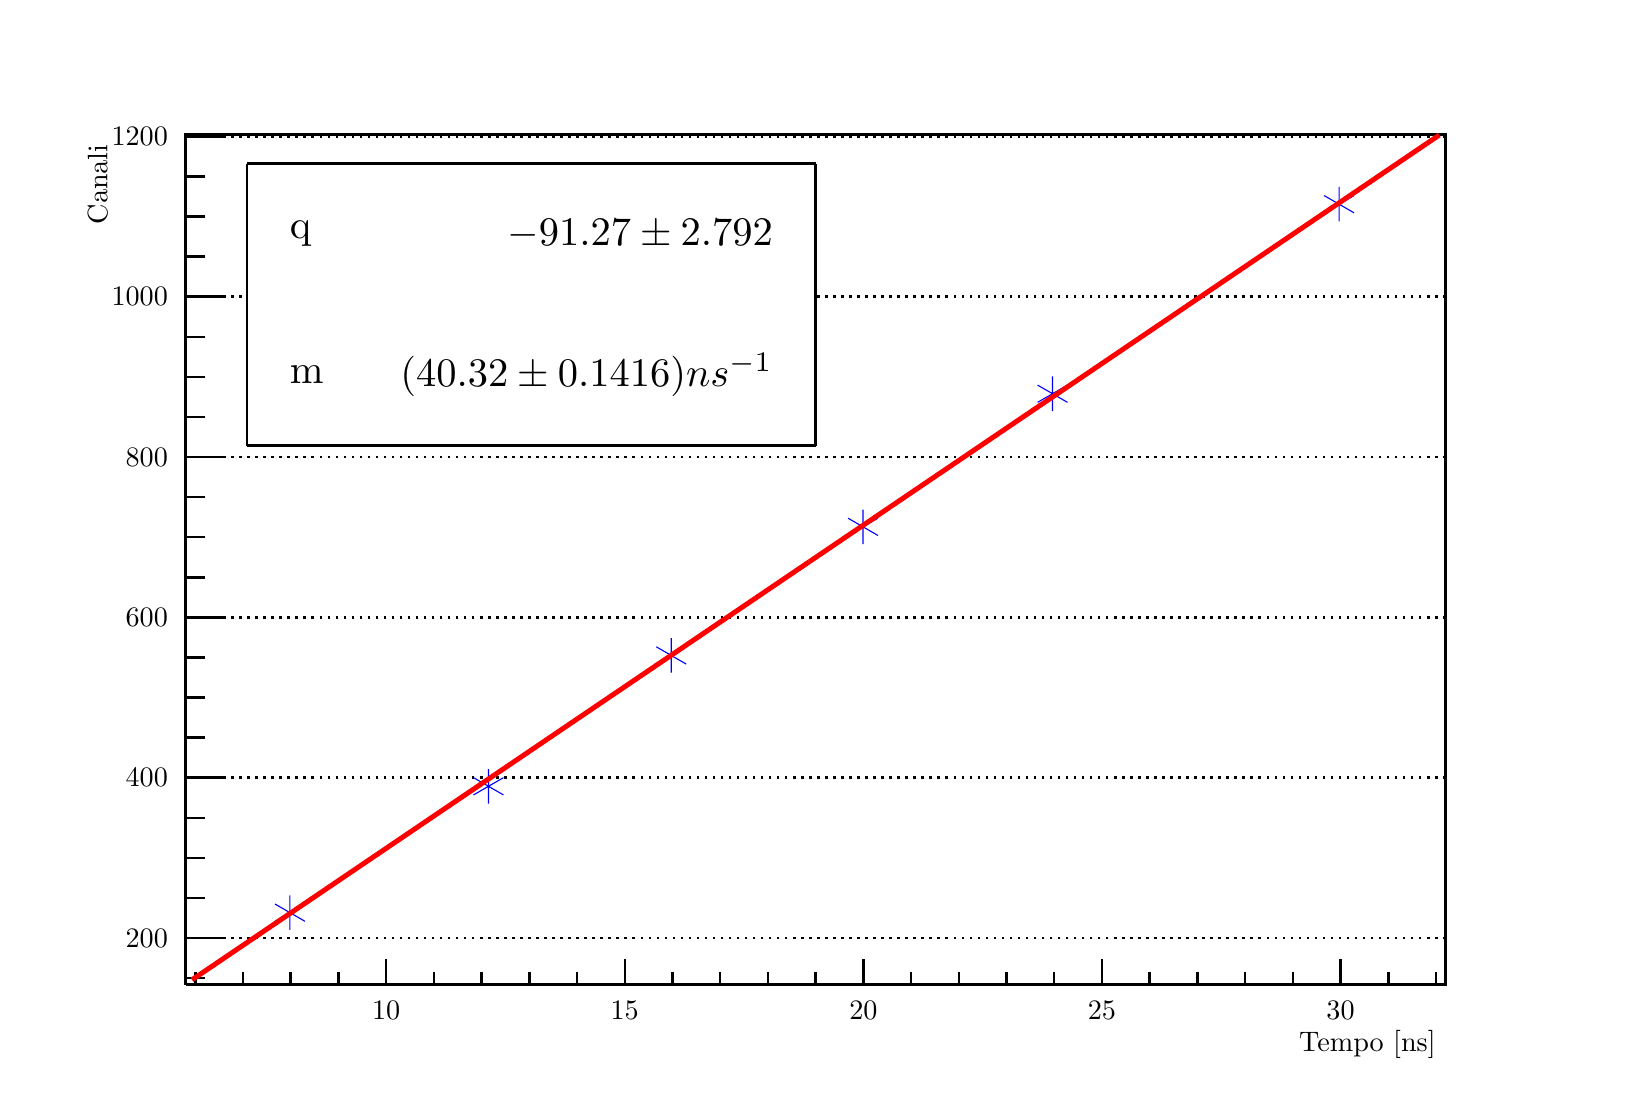
\begin{tikzpicture}
\pgfdeclareplotmark{cross} {
\pgfpathmoveto{\pgfpoint{-0.3\pgfplotmarksize}{\pgfplotmarksize}}
\pgfpathlineto{\pgfpoint{+0.3\pgfplotmarksize}{\pgfplotmarksize}}
\pgfpathlineto{\pgfpoint{+0.3\pgfplotmarksize}{0.3\pgfplotmarksize}}
\pgfpathlineto{\pgfpoint{+1\pgfplotmarksize}{0.3\pgfplotmarksize}}
\pgfpathlineto{\pgfpoint{+1\pgfplotmarksize}{-0.3\pgfplotmarksize}}
\pgfpathlineto{\pgfpoint{+0.3\pgfplotmarksize}{-0.3\pgfplotmarksize}}
\pgfpathlineto{\pgfpoint{+0.3\pgfplotmarksize}{-1.\pgfplotmarksize}}
\pgfpathlineto{\pgfpoint{-0.3\pgfplotmarksize}{-1.\pgfplotmarksize}}
\pgfpathlineto{\pgfpoint{-0.3\pgfplotmarksize}{-0.3\pgfplotmarksize}}
\pgfpathlineto{\pgfpoint{-1.\pgfplotmarksize}{-0.3\pgfplotmarksize}}
\pgfpathlineto{\pgfpoint{-1.\pgfplotmarksize}{0.3\pgfplotmarksize}}
\pgfpathlineto{\pgfpoint{-0.3\pgfplotmarksize}{0.3\pgfplotmarksize}}
\pgfpathclose
\pgfusepathqstroke
}
\pgfdeclareplotmark{cross*} {
\pgfpathmoveto{\pgfpoint{-0.3\pgfplotmarksize}{\pgfplotmarksize}}
\pgfpathlineto{\pgfpoint{+0.3\pgfplotmarksize}{\pgfplotmarksize}}
\pgfpathlineto{\pgfpoint{+0.3\pgfplotmarksize}{0.3\pgfplotmarksize}}
\pgfpathlineto{\pgfpoint{+1\pgfplotmarksize}{0.3\pgfplotmarksize}}
\pgfpathlineto{\pgfpoint{+1\pgfplotmarksize}{-0.3\pgfplotmarksize}}
\pgfpathlineto{\pgfpoint{+0.3\pgfplotmarksize}{-0.3\pgfplotmarksize}}
\pgfpathlineto{\pgfpoint{+0.3\pgfplotmarksize}{-1.\pgfplotmarksize}}
\pgfpathlineto{\pgfpoint{-0.3\pgfplotmarksize}{-1.\pgfplotmarksize}}
\pgfpathlineto{\pgfpoint{-0.3\pgfplotmarksize}{-0.3\pgfplotmarksize}}
\pgfpathlineto{\pgfpoint{-1.\pgfplotmarksize}{-0.3\pgfplotmarksize}}
\pgfpathlineto{\pgfpoint{-1.\pgfplotmarksize}{0.3\pgfplotmarksize}}
\pgfpathlineto{\pgfpoint{-0.3\pgfplotmarksize}{0.3\pgfplotmarksize}}
\pgfpathclose
\pgfusepathqfillstroke
}
\pgfdeclareplotmark{newstar} {
\pgfpathmoveto{\pgfqpoint{0pt}{\pgfplotmarksize}}
\pgfpathlineto{\pgfqpointpolar{44}{0.5\pgfplotmarksize}}
\pgfpathlineto{\pgfqpointpolar{18}{\pgfplotmarksize}}
\pgfpathlineto{\pgfqpointpolar{-20}{0.5\pgfplotmarksize}}
\pgfpathlineto{\pgfqpointpolar{-54}{\pgfplotmarksize}}
\pgfpathlineto{\pgfqpointpolar{-90}{0.5\pgfplotmarksize}}
\pgfpathlineto{\pgfqpointpolar{234}{\pgfplotmarksize}}
\pgfpathlineto{\pgfqpointpolar{198}{0.5\pgfplotmarksize}}
\pgfpathlineto{\pgfqpointpolar{162}{\pgfplotmarksize}}
\pgfpathlineto{\pgfqpointpolar{134}{0.5\pgfplotmarksize}}
\pgfpathclose
\pgfusepathqstroke
}
\pgfdeclareplotmark{newstar*} {
\pgfpathmoveto{\pgfqpoint{0pt}{\pgfplotmarksize}}
\pgfpathlineto{\pgfqpointpolar{44}{0.5\pgfplotmarksize}}
\pgfpathlineto{\pgfqpointpolar{18}{\pgfplotmarksize}}
\pgfpathlineto{\pgfqpointpolar{-20}{0.5\pgfplotmarksize}}
\pgfpathlineto{\pgfqpointpolar{-54}{\pgfplotmarksize}}
\pgfpathlineto{\pgfqpointpolar{-90}{0.5\pgfplotmarksize}}
\pgfpathlineto{\pgfqpointpolar{234}{\pgfplotmarksize}}
\pgfpathlineto{\pgfqpointpolar{198}{0.5\pgfplotmarksize}}
\pgfpathlineto{\pgfqpointpolar{162}{\pgfplotmarksize}}
\pgfpathlineto{\pgfqpointpolar{134}{0.5\pgfplotmarksize}}
\pgfpathclose
\pgfusepathqfillstroke
}
\definecolor{c}{rgb}{1,1,1};
\draw [color=c, fill=c] (0,0) rectangle (20,13.4957);
\draw [color=c, fill=c] (2,1.34957) rectangle (18,12.1461);
\definecolor{c}{rgb}{0,0,0};
\draw [c,line width=0.9] (2,1.34957) -- (2,12.1461) -- (18,12.1461) -- (18,1.34957) -- (2,1.34957);
\definecolor{c}{rgb}{1,1,1};
\draw [color=c, fill=c] (2,1.34957) rectangle (18,12.1461);
\definecolor{c}{rgb}{0,0,0};
\draw [c,line width=0.9] (2,1.34957) -- (2,12.1461) -- (18,12.1461) -- (18,1.34957) -- (2,1.34957);
\draw [c,line width=0.9] (2,1.34957) -- (18,1.34957);
\draw [c,line width=0.9] (2,1.34957) -- (2,12.1461);
\draw [c,dotted,line width=0.9] (18,1.94079) -- (2,1.94079);
\draw [c,dotted,line width=0.9] (18,3.97703) -- (2,3.97703);
\draw [c,dotted,line width=0.9] (18,6.01328) -- (2,6.01328);
\draw [c,dotted,line width=0.9] (18,8.04952) -- (2,8.04952);
\draw [c,dotted,line width=0.9] (18,10.0858) -- (2,10.0858);
\draw [c,dotted,line width=0.9] (18,12.122) -- (2,12.122);
\draw [c,dotted,line width=0.9] (18,1.94079) -- (2,1.94079);
\draw [c,dotted,line width=0.9] (18,12.122) -- (2,12.122);
\draw [c,line width=0.9] (2,1.34957) -- (18,1.34957);
\draw [anchor= east] (18,0.593811) node[scale=1.01821, color=c, rotate=0]{Tempo [ns]};
\draw [c,line width=0.9] (4.54545,1.67347) -- (4.54545,1.34957);
\draw [c,line width=0.9] (5.15152,1.51152) -- (5.15152,1.34957);
\draw [c,line width=0.9] (5.75758,1.51152) -- (5.75758,1.34957);
\draw [c,line width=0.9] (6.36364,1.51152) -- (6.36364,1.34957);
\draw [c,line width=0.9] (6.9697,1.51152) -- (6.9697,1.34957);
\draw [c,line width=0.9] (7.57576,1.67347) -- (7.57576,1.34957);
\draw [c,line width=0.9] (8.18182,1.51152) -- (8.18182,1.34957);
\draw [c,line width=0.9] (8.78788,1.51152) -- (8.78788,1.34957);
\draw [c,line width=0.9] (9.39394,1.51152) -- (9.39394,1.34957);
\draw [c,line width=0.9] (10,1.51152) -- (10,1.34957);
\draw [c,line width=0.9] (10.6061,1.67347) -- (10.6061,1.34957);
\draw [c,line width=0.9] (11.2121,1.51152) -- (11.2121,1.34957);
\draw [c,line width=0.9] (11.8182,1.51152) -- (11.8182,1.34957);
\draw [c,line width=0.9] (12.4242,1.51152) -- (12.4242,1.34957);
\draw [c,line width=0.9] (13.0303,1.51152) -- (13.0303,1.34957);
\draw [c,line width=0.9] (13.6364,1.67347) -- (13.6364,1.34957);
\draw [c,line width=0.9] (14.2424,1.51152) -- (14.2424,1.34957);
\draw [c,line width=0.9] (14.8485,1.51152) -- (14.8485,1.34957);
\draw [c,line width=0.9] (15.4545,1.51152) -- (15.4545,1.34957);
\draw [c,line width=0.9] (16.0606,1.51152) -- (16.0606,1.34957);
\draw [c,line width=0.9] (16.6667,1.67347) -- (16.6667,1.34957);
\draw [c,line width=0.9] (4.54545,1.67347) -- (4.54545,1.34957);
\draw [c,line width=0.9] (3.93939,1.51152) -- (3.93939,1.34957);
\draw [c,line width=0.9] (3.33333,1.51152) -- (3.33333,1.34957);
\draw [c,line width=0.9] (2.72727,1.51152) -- (2.72727,1.34957);
\draw [c,line width=0.9] (2.12121,1.51152) -- (2.12121,1.34957);
\draw [c,line width=0.9] (16.6667,1.67347) -- (16.6667,1.34957);
\draw [c,line width=0.9] (17.2727,1.51152) -- (17.2727,1.34957);
\draw [c,line width=0.9] (17.8788,1.51152) -- (17.8788,1.34957);
\draw [anchor=base] (4.54545,0.904212) node[scale=1.01821, color=c, rotate=0]{10};
\draw [anchor=base] (7.57576,0.904212) node[scale=1.01821, color=c, rotate=0]{15};
\draw [anchor=base] (10.6061,0.904212) node[scale=1.01821, color=c, rotate=0]{20};
\draw [anchor=base] (13.6364,0.904212) node[scale=1.01821, color=c, rotate=0]{25};
\draw [anchor=base] (16.6667,0.904212) node[scale=1.01821, color=c, rotate=0]{30};
\draw [c,line width=0.9] (2,1.34957) -- (2,12.1461);
\draw [anchor= east] (0.88,12.1461) node[scale=1.01821, color=c, rotate=90]{Canali};
\draw [c,line width=0.9] (2.48,1.94079) -- (2,1.94079);
\draw [c,line width=0.9] (2.24,2.44985) -- (2,2.44985);
\draw [c,line width=0.9] (2.24,2.95891) -- (2,2.95891);
\draw [c,line width=0.9] (2.24,3.46797) -- (2,3.46797);
\draw [c,line width=0.9] (2.48,3.97703) -- (2,3.97703);
\draw [c,line width=0.9] (2.24,4.4861) -- (2,4.4861);
\draw [c,line width=0.9] (2.24,4.99516) -- (2,4.99516);
\draw [c,line width=0.9] (2.24,5.50422) -- (2,5.50422);
\draw [c,line width=0.9] (2.48,6.01328) -- (2,6.01328);
\draw [c,line width=0.9] (2.24,6.52234) -- (2,6.52234);
\draw [c,line width=0.9] (2.24,7.0314) -- (2,7.0314);
\draw [c,line width=0.9] (2.24,7.54046) -- (2,7.54046);
\draw [c,line width=0.9] (2.48,8.04952) -- (2,8.04952);
\draw [c,line width=0.9] (2.24,8.55858) -- (2,8.55858);
\draw [c,line width=0.9] (2.24,9.06764) -- (2,9.06764);
\draw [c,line width=0.9] (2.24,9.5767) -- (2,9.5767);
\draw [c,line width=0.9] (2.48,10.0858) -- (2,10.0858);
\draw [c,line width=0.9] (2.24,10.5948) -- (2,10.5948);
\draw [c,line width=0.9] (2.24,11.1039) -- (2,11.1039);
\draw [c,line width=0.9] (2.24,11.6129) -- (2,11.6129);
\draw [c,line width=0.9] (2.48,12.122) -- (2,12.122);
\draw [c,line width=0.9] (2.48,1.94079) -- (2,1.94079);
\draw [c,line width=0.9] (2.24,1.43173) -- (2,1.43173);
\draw [c,line width=0.9] (2.48,12.122) -- (2,12.122);
\draw [anchor= east] (1.9,1.94079) node[scale=1.01821, color=c, rotate=0]{200};
\draw [anchor= east] (1.9,3.97703) node[scale=1.01821, color=c, rotate=0]{400};
\draw [anchor= east] (1.9,6.01328) node[scale=1.01821, color=c, rotate=0]{600};
\draw [anchor= east] (1.9,8.04952) node[scale=1.01821, color=c, rotate=0]{800};
\draw [anchor= east] (1.9,10.0858) node[scale=1.01821, color=c, rotate=0]{1000};
\draw [anchor= east] (1.9,12.122) node[scale=1.01821, color=c, rotate=0]{1200};
\definecolor{c}{rgb}{1,1,1};
\draw [color=c, fill=c] (2.77937,8.19484) rectangle (10,11.7765);
\definecolor{c}{rgb}{0,0,0};
\draw [c,line width=0.9] (2.77937,8.19484) -- (10,8.19484);
\draw [c,line width=0.9] (10,8.19484) -- (10,11.7765);
\draw [c,line width=0.9] (10,11.7765) -- (2.77937,11.7765);
\draw [c,line width=0.9] (2.77937,11.7765) -- (2.77937,8.19484);
\draw [anchor= west] (3.1404,10.8811) node[scale=1.46368, color=c, rotate=0]{q      };
\draw [anchor= east] (9.63897,10.8811) node[scale=1.46368, color=c, rotate=0]{$ -91.27 \pm 2.792$};
\draw [anchor= west] (3.1404,9.09026) node[scale=1.46368, color=c, rotate=0]{m       };
\draw [anchor= east] (9.63897,9.09026) node[scale=1.46368, color=c, rotate=0]{$ 40.32 \pm 0.1416$};
\definecolor{c}{rgb}{0,0,1};
\foreach \P in {(3.32378,2.26361),(5.84527,3.86819),(8.16619,5.53009),(10.6017,7.16332),(13.0086,8.85387),(16.6476,11.2607)}{\draw[mark options={color=c,fill=c},mark size=6.246246pt,mark=asterisk] plot coordinates {\P};}
\definecolor{c}{rgb}{1,0,0};
\draw [c,line width=1.8] (2.08,1.41032) -- (2.24,1.51869) -- (2.4,1.62706) -- (2.56,1.73543) -- (2.72,1.8438) -- (2.88,1.95217) -- (3.04,2.06054) -- (3.2,2.16891) -- (3.36,2.27728) -- (3.52,2.38564) -- (3.68,2.49401) -- (3.84,2.60238) -- (4,2.71075)
 -- (4.16,2.81912) -- (4.32,2.92749) -- (4.48,3.03586) -- (4.64,3.14423) -- (4.8,3.2526) -- (4.96,3.36097) -- (5.12,3.46934) -- (5.28,3.57771) -- (5.44,3.68608) -- (5.6,3.79445) -- (5.76,3.90282) -- (5.92,4.01119) -- (6.08,4.11956) -- (6.24,4.22793)
 -- (6.4,4.3363) -- (6.56,4.44467) -- (6.72,4.55303) -- (6.88,4.6614) -- (7.04,4.76977) -- (7.2,4.87814) -- (7.36,4.98651) -- (7.52,5.09488) -- (7.68,5.20325) -- (7.84,5.31162) -- (8,5.41999) -- (8.16,5.52836) -- (8.32,5.63673) -- (8.48,5.7451) --
 (8.64,5.85347) -- (8.8,5.96184) -- (8.96,6.07021) -- (9.12,6.17858) -- (9.28,6.28695) -- (9.44,6.39532) -- (9.6,6.50369) -- (9.76,6.61206) -- (9.92,6.72042);
\draw [c,line width=1.8] (9.92,6.72042) -- (10.08,6.82879) -- (10.24,6.93716) -- (10.4,7.04553) -- (10.56,7.1539) -- (10.72,7.26227) -- (10.88,7.37064) -- (11.04,7.47901) -- (11.2,7.58738) -- (11.36,7.69575) -- (11.52,7.80412) -- (11.68,7.91249) --
 (11.84,8.02086) -- (12,8.12923) -- (12.16,8.2376) -- (12.32,8.34597) -- (12.48,8.45434) -- (12.64,8.56271) -- (12.8,8.67108) -- (12.96,8.77944) -- (13.12,8.88781) -- (13.28,8.99618) -- (13.44,9.10455) -- (13.6,9.21292) -- (13.76,9.32129) --
 (13.92,9.42966) -- (14.08,9.53803) -- (14.24,9.6464) -- (14.4,9.75477) -- (14.56,9.86314) -- (14.72,9.97151) -- (14.88,10.0799) -- (15.04,10.1882) -- (15.2,10.2966) -- (15.36,10.405) -- (15.52,10.5134) -- (15.68,10.6217) -- (15.84,10.7301) --
 (16,10.8385) -- (16.16,10.9468) -- (16.32,11.0552) -- (16.48,11.1636) -- (16.64,11.2719) -- (16.8,11.3803) -- (16.96,11.4887) -- (17.12,11.5971) -- (17.28,11.7054) -- (17.44,11.8138) -- (17.6,11.9222) -- (17.76,12.0305);
\draw [c,line width=1.8] (17.76,12.0305) -- (17.92,12.1389);
\definecolor{c}{rgb}{1,1,1};
\draw [color=c, fill=c] (2.77937,8.19484) rectangle (10,11.7765);
\definecolor{c}{rgb}{0,0,0};
\draw [c,line width=0.9] (2.77937,8.19484) -- (10,8.19484);
\draw [c,line width=0.9] (10,8.19484) -- (10,11.7765);
\draw [c,line width=0.9] (10,11.7765) -- (2.77937,11.7765);
\draw [c,line width=0.9] (2.77937,11.7765) -- (2.77937,8.19484);
\draw [anchor= west] (3.1404,10.8811) node[scale=1.46368, color=c, rotate=0]{q       };
\draw [anchor= east] (9.63897,10.8811) node[scale=1.46368, color=c, rotate=0]{$ -91.27 \pm 2.792$};
\draw [anchor= west] (3.1404,9.09026) node[scale=1.46368, color=c, rotate=0]{m       };
\draw [anchor= east] (9.63897,9.09026) node[scale=1.46368, color=c, rotate=0]{$ (40.32 \pm 0.1416) ns^{-1}$};
%\draw (10.3438,12.6648) node[scale=1.40004, color=c, rotate=0]{Tempo vs Canali};
\end{tikzpicture}

%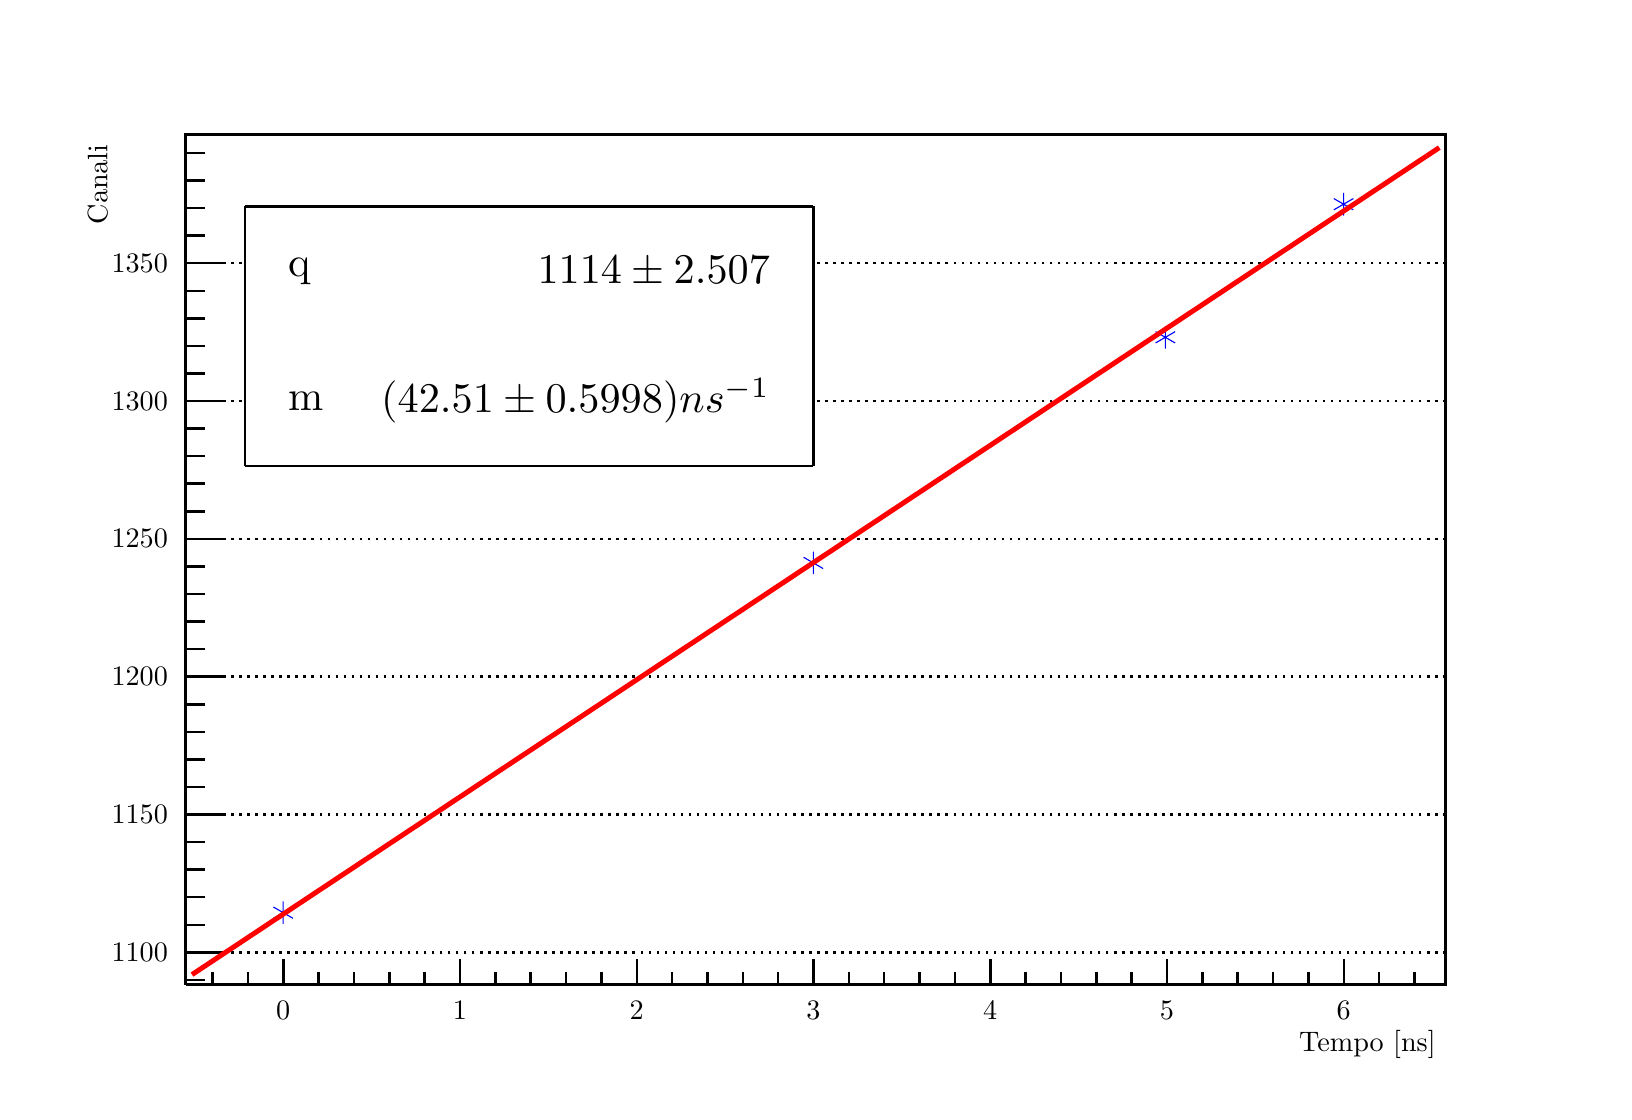
\begin{tikzpicture}
\pgfdeclareplotmark{cross} {
\pgfpathmoveto{\pgfpoint{-0.3\pgfplotmarksize}{\pgfplotmarksize}}
\pgfpathlineto{\pgfpoint{+0.3\pgfplotmarksize}{\pgfplotmarksize}}
\pgfpathlineto{\pgfpoint{+0.3\pgfplotmarksize}{0.3\pgfplotmarksize}}
\pgfpathlineto{\pgfpoint{+1\pgfplotmarksize}{0.3\pgfplotmarksize}}
\pgfpathlineto{\pgfpoint{+1\pgfplotmarksize}{-0.3\pgfplotmarksize}}
\pgfpathlineto{\pgfpoint{+0.3\pgfplotmarksize}{-0.3\pgfplotmarksize}}
\pgfpathlineto{\pgfpoint{+0.3\pgfplotmarksize}{-1.\pgfplotmarksize}}
\pgfpathlineto{\pgfpoint{-0.3\pgfplotmarksize}{-1.\pgfplotmarksize}}
\pgfpathlineto{\pgfpoint{-0.3\pgfplotmarksize}{-0.3\pgfplotmarksize}}
\pgfpathlineto{\pgfpoint{-1.\pgfplotmarksize}{-0.3\pgfplotmarksize}}
\pgfpathlineto{\pgfpoint{-1.\pgfplotmarksize}{0.3\pgfplotmarksize}}
\pgfpathlineto{\pgfpoint{-0.3\pgfplotmarksize}{0.3\pgfplotmarksize}}
\pgfpathclose
\pgfusepathqstroke
}
\pgfdeclareplotmark{cross*} {
\pgfpathmoveto{\pgfpoint{-0.3\pgfplotmarksize}{\pgfplotmarksize}}
\pgfpathlineto{\pgfpoint{+0.3\pgfplotmarksize}{\pgfplotmarksize}}
\pgfpathlineto{\pgfpoint{+0.3\pgfplotmarksize}{0.3\pgfplotmarksize}}
\pgfpathlineto{\pgfpoint{+1\pgfplotmarksize}{0.3\pgfplotmarksize}}
\pgfpathlineto{\pgfpoint{+1\pgfplotmarksize}{-0.3\pgfplotmarksize}}
\pgfpathlineto{\pgfpoint{+0.3\pgfplotmarksize}{-0.3\pgfplotmarksize}}
\pgfpathlineto{\pgfpoint{+0.3\pgfplotmarksize}{-1.\pgfplotmarksize}}
\pgfpathlineto{\pgfpoint{-0.3\pgfplotmarksize}{-1.\pgfplotmarksize}}
\pgfpathlineto{\pgfpoint{-0.3\pgfplotmarksize}{-0.3\pgfplotmarksize}}
\pgfpathlineto{\pgfpoint{-1.\pgfplotmarksize}{-0.3\pgfplotmarksize}}
\pgfpathlineto{\pgfpoint{-1.\pgfplotmarksize}{0.3\pgfplotmarksize}}
\pgfpathlineto{\pgfpoint{-0.3\pgfplotmarksize}{0.3\pgfplotmarksize}}
\pgfpathclose
\pgfusepathqfillstroke
}
\pgfdeclareplotmark{newstar} {
\pgfpathmoveto{\pgfqpoint{0pt}{\pgfplotmarksize}}
\pgfpathlineto{\pgfqpointpolar{44}{0.5\pgfplotmarksize}}
\pgfpathlineto{\pgfqpointpolar{18}{\pgfplotmarksize}}
\pgfpathlineto{\pgfqpointpolar{-20}{0.5\pgfplotmarksize}}
\pgfpathlineto{\pgfqpointpolar{-54}{\pgfplotmarksize}}
\pgfpathlineto{\pgfqpointpolar{-90}{0.5\pgfplotmarksize}}
\pgfpathlineto{\pgfqpointpolar{234}{\pgfplotmarksize}}
\pgfpathlineto{\pgfqpointpolar{198}{0.5\pgfplotmarksize}}
\pgfpathlineto{\pgfqpointpolar{162}{\pgfplotmarksize}}
\pgfpathlineto{\pgfqpointpolar{134}{0.5\pgfplotmarksize}}
\pgfpathclose
\pgfusepathqstroke
}
\pgfdeclareplotmark{newstar*} {
\pgfpathmoveto{\pgfqpoint{0pt}{\pgfplotmarksize}}
\pgfpathlineto{\pgfqpointpolar{44}{0.5\pgfplotmarksize}}
\pgfpathlineto{\pgfqpointpolar{18}{\pgfplotmarksize}}
\pgfpathlineto{\pgfqpointpolar{-20}{0.5\pgfplotmarksize}}
\pgfpathlineto{\pgfqpointpolar{-54}{\pgfplotmarksize}}
\pgfpathlineto{\pgfqpointpolar{-90}{0.5\pgfplotmarksize}}
\pgfpathlineto{\pgfqpointpolar{234}{\pgfplotmarksize}}
\pgfpathlineto{\pgfqpointpolar{198}{0.5\pgfplotmarksize}}
\pgfpathlineto{\pgfqpointpolar{162}{\pgfplotmarksize}}
\pgfpathlineto{\pgfqpointpolar{134}{0.5\pgfplotmarksize}}
\pgfpathclose
\pgfusepathqfillstroke
}
\definecolor{c}{rgb}{1,1,1};
\draw [color=c, fill=c] (0,0) rectangle (20,13.4957);
\draw [color=c, fill=c] (2,1.34957) rectangle (18,12.1461);
\definecolor{c}{rgb}{0,0,0};
\draw [c,line width=0.9] (2,1.34957) -- (2,12.1461) -- (18,12.1461) -- (18,1.34957) -- (2,1.34957);
\definecolor{c}{rgb}{1,1,1};
\draw [color=c, fill=c] (2,1.34957) rectangle (18,12.1461);
\definecolor{c}{rgb}{0,0,0};
\draw [c,line width=0.9] (2,1.34957) -- (2,12.1461) -- (18,12.1461) -- (18,1.34957) -- (2,1.34957);
\draw [c,line width=0.9] (2,1.34957) -- (18,1.34957);
\draw [c,line width=0.9] (2,1.34957) -- (2,12.1461);
\draw [c,dotted,line width=0.9] (18,1.75917) -- (2,1.75917);
\draw [c,dotted,line width=0.9] (18,3.50958) -- (2,3.50958);
\draw [c,dotted,line width=0.9] (18,5.26) -- (2,5.26);
\draw [c,dotted,line width=0.9] (18,7.01041) -- (2,7.01041);
\draw [c,dotted,line width=0.9] (18,8.76083) -- (2,8.76083);
\draw [c,dotted,line width=0.9] (18,10.5112) -- (2,10.5112);
\draw [c,dotted,line width=0.9] (18,1.75917) -- (2,1.75917);
\draw [c,dotted,line width=0.9] (18,10.5112) -- (2,10.5112);
\draw [c,line width=0.9] (2,1.34957) -- (18,1.34957);
\draw [anchor= east] (18,0.593811) node[scale=1.01821, color=c, rotate=0]{Tempo [ns]};
\draw [c,line width=0.9] (3.23906,1.67347) -- (3.23906,1.34957);
\draw [c,line width=0.9] (3.68799,1.51152) -- (3.68799,1.34957);
\draw [c,line width=0.9] (4.13692,1.51152) -- (4.13692,1.34957);
\draw [c,line width=0.9] (4.58586,1.51152) -- (4.58586,1.34957);
\draw [c,line width=0.9] (5.03479,1.51152) -- (5.03479,1.34957);
\draw [c,line width=0.9] (5.48373,1.67347) -- (5.48373,1.34957);
\draw [c,line width=0.9] (5.93266,1.51152) -- (5.93266,1.34957);
\draw [c,line width=0.9] (6.38159,1.51152) -- (6.38159,1.34957);
\draw [c,line width=0.9] (6.83053,1.51152) -- (6.83053,1.34957);
\draw [c,line width=0.9] (7.27946,1.51152) -- (7.27946,1.34957);
\draw [c,line width=0.9] (7.72839,1.67347) -- (7.72839,1.34957);
\draw [c,line width=0.9] (8.17733,1.51152) -- (8.17733,1.34957);
\draw [c,line width=0.9] (8.62626,1.51152) -- (8.62626,1.34957);
\draw [c,line width=0.9] (9.0752,1.51152) -- (9.0752,1.34957);
\draw [c,line width=0.9] (9.52413,1.51152) -- (9.52413,1.34957);
\draw [c,line width=0.9] (9.97306,1.67347) -- (9.97306,1.34957);
\draw [c,line width=0.9] (10.422,1.51152) -- (10.422,1.34957);
\draw [c,line width=0.9] (10.8709,1.51152) -- (10.8709,1.34957);
\draw [c,line width=0.9] (11.3199,1.51152) -- (11.3199,1.34957);
\draw [c,line width=0.9] (11.7688,1.51152) -- (11.7688,1.34957);
\draw [c,line width=0.9] (12.2177,1.67347) -- (12.2177,1.34957);
\draw [c,line width=0.9] (12.6667,1.51152) -- (12.6667,1.34957);
\draw [c,line width=0.9] (13.1156,1.51152) -- (13.1156,1.34957);
\draw [c,line width=0.9] (13.5645,1.51152) -- (13.5645,1.34957);
\draw [c,line width=0.9] (14.0135,1.51152) -- (14.0135,1.34957);
\draw [c,line width=0.9] (14.4624,1.67347) -- (14.4624,1.34957);
\draw [c,line width=0.9] (14.9113,1.51152) -- (14.9113,1.34957);
\draw [c,line width=0.9] (15.3603,1.51152) -- (15.3603,1.34957);
\draw [c,line width=0.9] (15.8092,1.51152) -- (15.8092,1.34957);
\draw [c,line width=0.9] (16.2581,1.51152) -- (16.2581,1.34957);
\draw [c,line width=0.9] (16.7071,1.67347) -- (16.7071,1.34957);
\draw [c,line width=0.9] (3.23906,1.67347) -- (3.23906,1.34957);
\draw [c,line width=0.9] (2.79012,1.51152) -- (2.79012,1.34957);
\draw [c,line width=0.9] (2.34119,1.51152) -- (2.34119,1.34957);
\draw [c,line width=0.9] (16.7071,1.67347) -- (16.7071,1.34957);
\draw [c,line width=0.9] (17.156,1.51152) -- (17.156,1.34957);
\draw [c,line width=0.9] (17.6049,1.51152) -- (17.6049,1.34957);
\draw [anchor=base] (3.23906,0.904212) node[scale=1.01821, color=c, rotate=0]{0};
\draw [anchor=base] (5.48373,0.904212) node[scale=1.01821, color=c, rotate=0]{1};
\draw [anchor=base] (7.72839,0.904212) node[scale=1.01821, color=c, rotate=0]{2};
\draw [anchor=base] (9.97306,0.904212) node[scale=1.01821, color=c, rotate=0]{3};
\draw [anchor=base] (12.2177,0.904212) node[scale=1.01821, color=c, rotate=0]{4};
\draw [anchor=base] (14.4624,0.904212) node[scale=1.01821, color=c, rotate=0]{5};
\draw [anchor=base] (16.7071,0.904212) node[scale=1.01821, color=c, rotate=0]{6};
\draw [c,line width=0.9] (2,1.34957) -- (2,12.1461);
\draw [anchor= east] (0.88,12.1461) node[scale=1.01821, color=c, rotate=90]{Canali};
\draw [c,line width=0.9] (2.48,1.75917) -- (2,1.75917);
\draw [c,line width=0.9] (2.24,2.10925) -- (2,2.10925);
\draw [c,line width=0.9] (2.24,2.45933) -- (2,2.45933);
\draw [c,line width=0.9] (2.24,2.80942) -- (2,2.80942);
\draw [c,line width=0.9] (2.24,3.1595) -- (2,3.1595);
\draw [c,line width=0.9] (2.48,3.50958) -- (2,3.50958);
\draw [c,line width=0.9] (2.24,3.85967) -- (2,3.85967);
\draw [c,line width=0.9] (2.24,4.20975) -- (2,4.20975);
\draw [c,line width=0.9] (2.24,4.55983) -- (2,4.55983);
\draw [c,line width=0.9] (2.24,4.90991) -- (2,4.90991);
\draw [c,line width=0.9] (2.48,5.26) -- (2,5.26);
\draw [c,line width=0.9] (2.24,5.61008) -- (2,5.61008);
\draw [c,line width=0.9] (2.24,5.96016) -- (2,5.96016);
\draw [c,line width=0.9] (2.24,6.31025) -- (2,6.31025);
\draw [c,line width=0.9] (2.24,6.66033) -- (2,6.66033);
\draw [c,line width=0.9] (2.48,7.01041) -- (2,7.01041);
\draw [c,line width=0.9] (2.24,7.3605) -- (2,7.3605);
\draw [c,line width=0.9] (2.24,7.71058) -- (2,7.71058);
\draw [c,line width=0.9] (2.24,8.06066) -- (2,8.06066);
\draw [c,line width=0.9] (2.24,8.41075) -- (2,8.41075);
\draw [c,line width=0.9] (2.48,8.76083) -- (2,8.76083);
\draw [c,line width=0.9] (2.24,9.11091) -- (2,9.11091);
\draw [c,line width=0.9] (2.24,9.46099) -- (2,9.46099);
\draw [c,line width=0.9] (2.24,9.81108) -- (2,9.81108);
\draw [c,line width=0.9] (2.24,10.1612) -- (2,10.1612);
\draw [c,line width=0.9] (2.48,10.5112) -- (2,10.5112);
\draw [c,line width=0.9] (2.48,1.75917) -- (2,1.75917);
\draw [c,line width=0.9] (2.24,1.40908) -- (2,1.40908);
\draw [c,line width=0.9] (2.48,10.5112) -- (2,10.5112);
\draw [c,line width=0.9] (2.24,10.8613) -- (2,10.8613);
\draw [c,line width=0.9] (2.24,11.2114) -- (2,11.2114);
\draw [c,line width=0.9] (2.24,11.5615) -- (2,11.5615);
\draw [c,line width=0.9] (2.24,11.9116) -- (2,11.9116);
\draw [anchor= east] (1.9,1.75917) node[scale=1.01821, color=c, rotate=0]{1100};
\draw [anchor= east] (1.9,3.50958) node[scale=1.01821, color=c, rotate=0]{1150};
\draw [anchor= east] (1.9,5.26) node[scale=1.01821, color=c, rotate=0]{1200};
\draw [anchor= east] (1.9,7.01041) node[scale=1.01821, color=c, rotate=0]{1250};
\draw [anchor= east] (1.9,8.76083) node[scale=1.01821, color=c, rotate=0]{1300};
\draw [anchor= east] (1.9,10.5112) node[scale=1.01821, color=c, rotate=0]{1350};
\definecolor{c}{rgb}{1,1,1};
\draw [color=c, fill=c] (2.75072,7.93696) rectangle (9.97135,11.2321);
\definecolor{c}{rgb}{0,0,0};
\draw [c,line width=0.9] (2.75072,7.93696) -- (9.97135,7.93696);
\draw [c,line width=0.9] (9.97135,7.93696) -- (9.97135,11.2321);
\draw [c,line width=0.9] (9.97135,11.2321) -- (2.75072,11.2321);
\draw [c,line width=0.9] (2.75072,11.2321) -- (2.75072,7.93696);
\draw [anchor= west] (3.11175,10.4083) node[scale=1.52731, color=c, rotate=0]{q       };
\draw [anchor= east] (9.61032,10.4083) node[scale=1.52731, color=c, rotate=0]{$  1114 \pm 2.507$};
\draw [anchor= west] (3.11175,8.76075) node[scale=1.52731, color=c, rotate=0]{m       };
\draw [anchor= east] (9.61032,8.76075) node[scale=1.52731, color=c, rotate=0]{$ 42.51 \pm 0.5998$};
\definecolor{c}{rgb}{0,0,1};
\foreach \P in {(3.23782,2.26361),(9.97135,6.70487),(14.4413,9.5702),(16.7049,11.2607)}{\draw[mark options={color=c,fill=c},mark size=4.084084pt,mark=asterisk] plot coordinates {\P};}
\definecolor{c}{rgb}{1,0,0};
\draw [c,line width=1.8] (2.08,1.47669) -- (2.24,1.58277) -- (2.4,1.68886) -- (2.56,1.79494) -- (2.72,1.90103) -- (2.88,2.00711) -- (3.04,2.1132) -- (3.2,2.21929) -- (3.36,2.32537) -- (3.52,2.43146) -- (3.68,2.53754) -- (3.84,2.64363) -- (4,2.74971)
 -- (4.16,2.8558) -- (4.32,2.96189) -- (4.48,3.06797) -- (4.64,3.17406) -- (4.8,3.28014) -- (4.96,3.38623) -- (5.12,3.49231) -- (5.28,3.5984) -- (5.44,3.70448) -- (5.6,3.81057) -- (5.76,3.91666) -- (5.92,4.02274) -- (6.08,4.12883) -- (6.24,4.23491)
 -- (6.4,4.341) -- (6.56,4.44708) -- (6.72,4.55317) -- (6.88,4.65926) -- (7.04,4.76534) -- (7.2,4.87143) -- (7.36,4.97751) -- (7.52,5.0836) -- (7.68,5.18968) -- (7.84,5.29577) -- (8,5.40186) -- (8.16,5.50794) -- (8.32,5.61403) -- (8.48,5.72011) --
 (8.64,5.8262) -- (8.8,5.93228) -- (8.96,6.03837) -- (9.12,6.14446) -- (9.28,6.25054) -- (9.44,6.35663) -- (9.6,6.46271) -- (9.76,6.5688) -- (9.92,6.67488);
\draw [c,line width=1.8] (9.92,6.67488) -- (10.08,6.78097) -- (10.24,6.88706) -- (10.4,6.99314) -- (10.56,7.09923) -- (10.72,7.20531) -- (10.88,7.3114) -- (11.04,7.41748) -- (11.2,7.52357) -- (11.36,7.62965) -- (11.52,7.73574) -- (11.68,7.84183) --
 (11.84,7.94791) -- (12,8.054) -- (12.16,8.16008) -- (12.32,8.26617) -- (12.48,8.37226) -- (12.64,8.47834) -- (12.8,8.58443) -- (12.96,8.69051) -- (13.12,8.7966) -- (13.28,8.90268) -- (13.44,9.00877) -- (13.6,9.11485) -- (13.76,9.22094) --
 (13.92,9.32703) -- (14.08,9.43311) -- (14.24,9.5392) -- (14.4,9.64528) -- (14.56,9.75137) -- (14.72,9.85745) -- (14.88,9.96354) -- (15.04,10.0696) -- (15.2,10.1757) -- (15.36,10.2818) -- (15.52,10.3879) -- (15.68,10.494) -- (15.84,10.6001) --
 (16,10.7061) -- (16.16,10.8122) -- (16.32,10.9183) -- (16.48,11.0244) -- (16.64,11.1305) -- (16.8,11.2366) -- (16.96,11.3427) -- (17.12,11.4487) -- (17.28,11.5548) -- (17.44,11.6609) -- (17.6,11.767) -- (17.76,11.8731);
\draw [c,line width=1.8] (17.76,11.8731) -- (17.92,11.9792);
\definecolor{c}{rgb}{1,1,1};
\draw [color=c, fill=c] (2.75072,7.93696) rectangle (9.97135,11.2321);
\definecolor{c}{rgb}{0,0,0};
\draw [c,line width=0.9] (2.75072,7.93696) -- (9.97135,7.93696);
\draw [c,line width=0.9] (9.97135,7.93696) -- (9.97135,11.2321);
\draw [c,line width=0.9] (9.97135,11.2321) -- (2.75072,11.2321);
\draw [c,line width=0.9] (2.75072,11.2321) -- (2.75072,7.93696);
\draw [anchor= west] (3.11175,10.4083) node[scale=1.52731, color=c, rotate=0]{q       };
\draw [anchor= east] (9.61032,10.4083) node[scale=1.52731, color=c, rotate=0]{$  1114 \pm 2.507$};
\draw [anchor= west] (3.11175,8.76075) node[scale=1.52731, color=c, rotate=0]{m       };
\draw [anchor= east] (9.61032,8.76075) node[scale=1.52731, color=c, rotate=0]{$ (42.51 \pm 0.5998) ns^{-1}$};
%\draw (9.55587,12.808) node[scale=1.40004, color=c, rotate=0]{Calibrazione Cavi};
\end{tikzpicture}


La dipendenza lineare attesa è stata ben riscontrata.
A seguito di tale calibrazione è stato possibile ricavare il ritardo associato all'inserimento di cavi LEMO tra il Delay e lo stop del TAC ricavando il centroide dai vari spettri del 
TAC ed associandovi un ritardo ricavato tramite i parametri del precedente fit. La relazione lineare che vede in ascissa i tempi ed i relativi centroidi in ordinata è stata 
quindi invertita ricavandosi per propagazione gli errori sui nuovi parametri ed ottenendo i seguenti risultati. Il ritardo associato ai cavetti di diversa lunghezza è molto simile
a quello indicato, la differenza è forse dovuta ad approssimazioni o ad effetti strumentali.\\

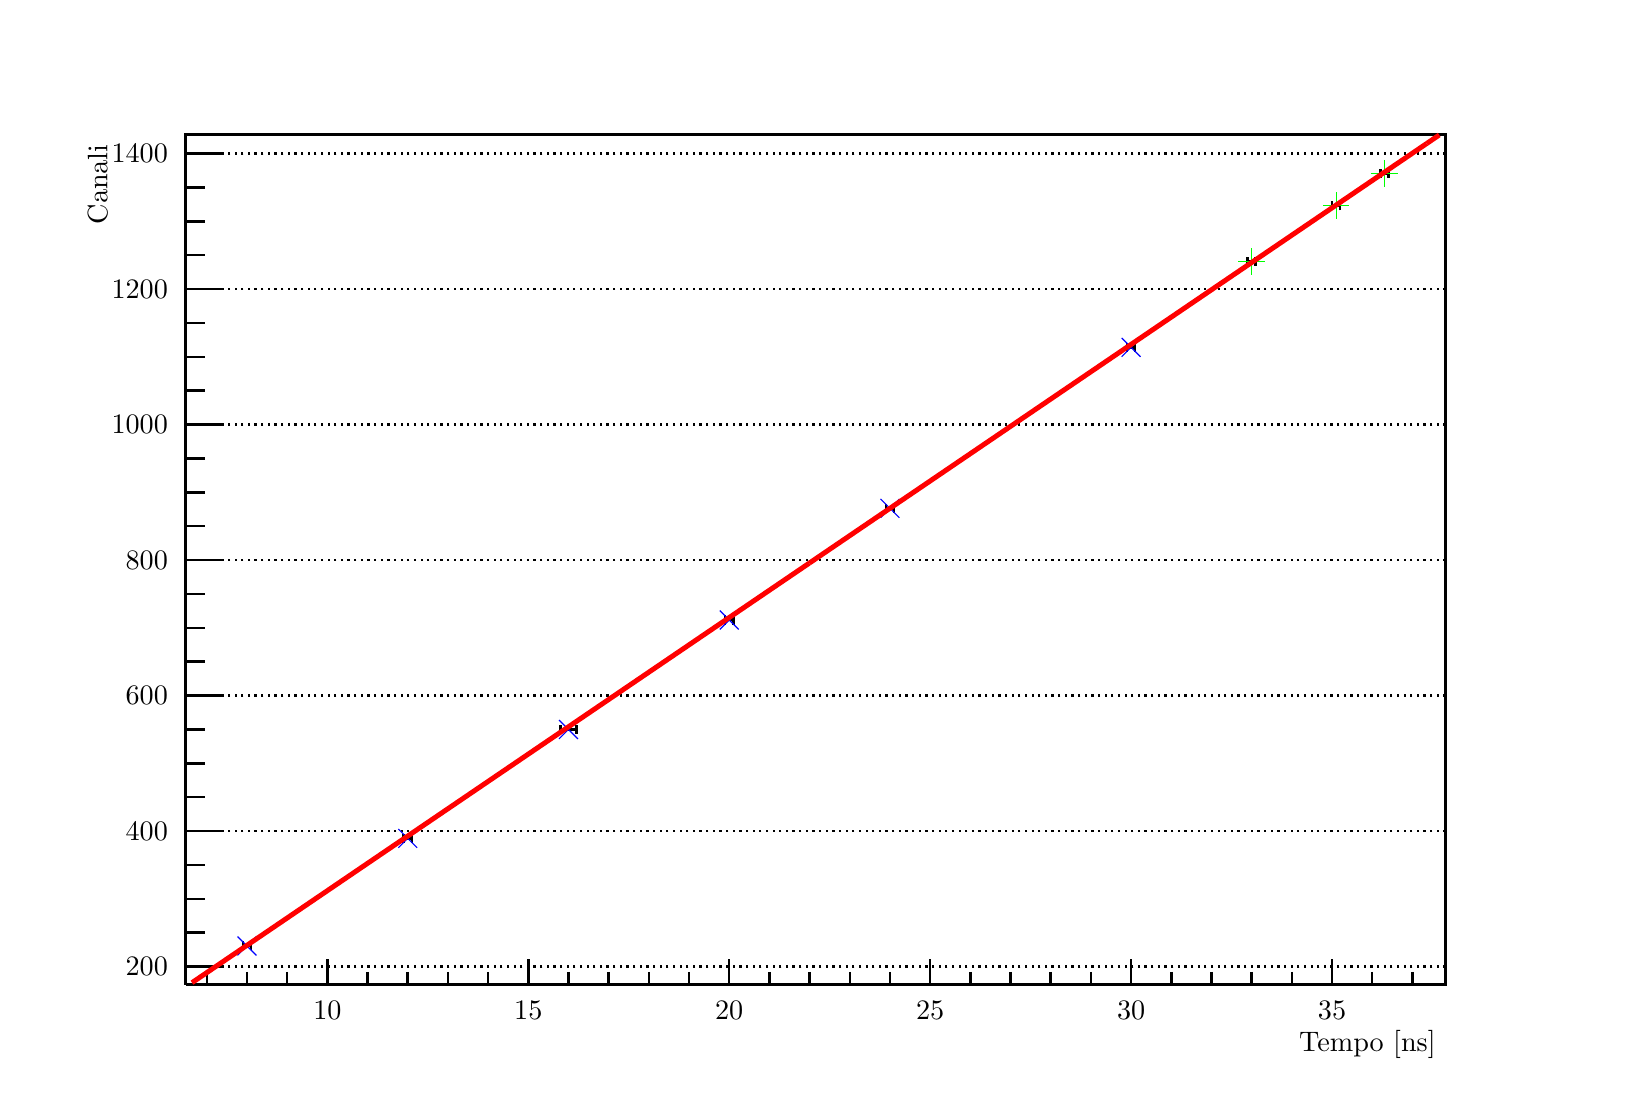
\begin{tikzpicture}
\pgfdeclareplotmark{cross} {
\pgfpathmoveto{\pgfpoint{-0.3\pgfplotmarksize}{\pgfplotmarksize}}
\pgfpathlineto{\pgfpoint{+0.3\pgfplotmarksize}{\pgfplotmarksize}}
\pgfpathlineto{\pgfpoint{+0.3\pgfplotmarksize}{0.3\pgfplotmarksize}}
\pgfpathlineto{\pgfpoint{+1\pgfplotmarksize}{0.3\pgfplotmarksize}}
\pgfpathlineto{\pgfpoint{+1\pgfplotmarksize}{-0.3\pgfplotmarksize}}
\pgfpathlineto{\pgfpoint{+0.3\pgfplotmarksize}{-0.3\pgfplotmarksize}}
\pgfpathlineto{\pgfpoint{+0.3\pgfplotmarksize}{-1.\pgfplotmarksize}}
\pgfpathlineto{\pgfpoint{-0.3\pgfplotmarksize}{-1.\pgfplotmarksize}}
\pgfpathlineto{\pgfpoint{-0.3\pgfplotmarksize}{-0.3\pgfplotmarksize}}
\pgfpathlineto{\pgfpoint{-1.\pgfplotmarksize}{-0.3\pgfplotmarksize}}
\pgfpathlineto{\pgfpoint{-1.\pgfplotmarksize}{0.3\pgfplotmarksize}}
\pgfpathlineto{\pgfpoint{-0.3\pgfplotmarksize}{0.3\pgfplotmarksize}}
\pgfpathclose
\pgfusepathqstroke
}
\pgfdeclareplotmark{cross*} {
\pgfpathmoveto{\pgfpoint{-0.3\pgfplotmarksize}{\pgfplotmarksize}}
\pgfpathlineto{\pgfpoint{+0.3\pgfplotmarksize}{\pgfplotmarksize}}
\pgfpathlineto{\pgfpoint{+0.3\pgfplotmarksize}{0.3\pgfplotmarksize}}
\pgfpathlineto{\pgfpoint{+1\pgfplotmarksize}{0.3\pgfplotmarksize}}
\pgfpathlineto{\pgfpoint{+1\pgfplotmarksize}{-0.3\pgfplotmarksize}}
\pgfpathlineto{\pgfpoint{+0.3\pgfplotmarksize}{-0.3\pgfplotmarksize}}
\pgfpathlineto{\pgfpoint{+0.3\pgfplotmarksize}{-1.\pgfplotmarksize}}
\pgfpathlineto{\pgfpoint{-0.3\pgfplotmarksize}{-1.\pgfplotmarksize}}
\pgfpathlineto{\pgfpoint{-0.3\pgfplotmarksize}{-0.3\pgfplotmarksize}}
\pgfpathlineto{\pgfpoint{-1.\pgfplotmarksize}{-0.3\pgfplotmarksize}}
\pgfpathlineto{\pgfpoint{-1.\pgfplotmarksize}{0.3\pgfplotmarksize}}
\pgfpathlineto{\pgfpoint{-0.3\pgfplotmarksize}{0.3\pgfplotmarksize}}
\pgfpathclose
\pgfusepathqfillstroke
}
\pgfdeclareplotmark{newstar} {
\pgfpathmoveto{\pgfqpoint{0pt}{\pgfplotmarksize}}
\pgfpathlineto{\pgfqpointpolar{44}{0.5\pgfplotmarksize}}
\pgfpathlineto{\pgfqpointpolar{18}{\pgfplotmarksize}}
\pgfpathlineto{\pgfqpointpolar{-20}{0.5\pgfplotmarksize}}
\pgfpathlineto{\pgfqpointpolar{-54}{\pgfplotmarksize}}
\pgfpathlineto{\pgfqpointpolar{-90}{0.5\pgfplotmarksize}}
\pgfpathlineto{\pgfqpointpolar{234}{\pgfplotmarksize}}
\pgfpathlineto{\pgfqpointpolar{198}{0.5\pgfplotmarksize}}
\pgfpathlineto{\pgfqpointpolar{162}{\pgfplotmarksize}}
\pgfpathlineto{\pgfqpointpolar{134}{0.5\pgfplotmarksize}}
\pgfpathclose
\pgfusepathqstroke
}
\pgfdeclareplotmark{newstar*} {
\pgfpathmoveto{\pgfqpoint{0pt}{\pgfplotmarksize}}
\pgfpathlineto{\pgfqpointpolar{44}{0.5\pgfplotmarksize}}
\pgfpathlineto{\pgfqpointpolar{18}{\pgfplotmarksize}}
\pgfpathlineto{\pgfqpointpolar{-20}{0.5\pgfplotmarksize}}
\pgfpathlineto{\pgfqpointpolar{-54}{\pgfplotmarksize}}
\pgfpathlineto{\pgfqpointpolar{-90}{0.5\pgfplotmarksize}}
\pgfpathlineto{\pgfqpointpolar{234}{\pgfplotmarksize}}
\pgfpathlineto{\pgfqpointpolar{198}{0.5\pgfplotmarksize}}
\pgfpathlineto{\pgfqpointpolar{162}{\pgfplotmarksize}}
\pgfpathlineto{\pgfqpointpolar{134}{0.5\pgfplotmarksize}}
\pgfpathclose
\pgfusepathqfillstroke
}
\definecolor{c}{rgb}{1,1,1};
\draw [color=c, fill=c] (0,0) rectangle (20,13.4957);
\draw [color=c, fill=c] (2,1.34957) rectangle (18,12.1461);
\definecolor{c}{rgb}{0,0,0};
\draw [c,line width=0.9] (2,1.34957) -- (2,12.1461) -- (18,12.1461) -- (18,1.34957) -- (2,1.34957);
\definecolor{c}{rgb}{1,1,1};
\draw [color=c, fill=c] (2,1.34957) rectangle (18,12.1461);
\definecolor{c}{rgb}{0,0,0};
\draw [c,line width=0.9] (2,1.34957) -- (2,12.1461) -- (18,12.1461) -- (18,1.34957) -- (2,1.34957);
\draw [c,line width=0.9] (2,1.34957) -- (18,1.34957);
\draw [c,line width=0.9] (2,1.34957) -- (2,12.1461);
\draw [c,dash pattern=on 0.80pt off 1.60pt ,line width=0.9] (18,1.57966) -- (2,1.57966);
\draw [c,dash pattern=on 0.80pt off 1.60pt ,line width=0.9] (18,3.30024) -- (2,3.30024);
\draw [c,dash pattern=on 0.80pt off 1.60pt ,line width=0.9] (18,5.02082) -- (2,5.02082);
\draw [c,dash pattern=on 0.80pt off 1.60pt ,line width=0.9] (18,6.7414) -- (2,6.7414);
\draw [c,dash pattern=on 0.80pt off 1.60pt ,line width=0.9] (18,8.46198) -- (2,8.46198);
\draw [c,dash pattern=on 0.80pt off 1.60pt ,line width=0.9] (18,10.1826) -- (2,10.1826);
\draw [c,dash pattern=on 0.80pt off 1.60pt ,line width=0.9] (18,11.9031) -- (2,11.9031);
\draw [c,dash pattern=on 0.80pt off 1.60pt ,line width=0.9] (18,1.57966) -- (2,1.57966);
\draw [c,dash pattern=on 0.80pt off 1.60pt ,line width=0.9] (18,11.9031) -- (2,11.9031);
\draw [c,line width=0.9] (2,1.34957) -- (18,1.34957);
\draw [anchor= east] (18,0.593811) node[scale=1.01821, color=c, rotate=0]{Tempo [ns]};
\draw [c,line width=0.9] (3.79904,1.67347) -- (3.79904,1.34957);
\draw [c,line width=0.9] (4.30941,1.51152) -- (4.30941,1.34957);
\draw [c,line width=0.9] (4.81978,1.51152) -- (4.81978,1.34957);
\draw [c,line width=0.9] (5.33014,1.51152) -- (5.33014,1.34957);
\draw [c,line width=0.9] (5.84051,1.51152) -- (5.84051,1.34957);
\draw [c,line width=0.9] (6.35088,1.67347) -- (6.35088,1.34957);
\draw [c,line width=0.9] (6.86124,1.51152) -- (6.86124,1.34957);
\draw [c,line width=0.9] (7.37161,1.51152) -- (7.37161,1.34957);
\draw [c,line width=0.9] (7.88198,1.51152) -- (7.88198,1.34957);
\draw [c,line width=0.9] (8.39234,1.51152) -- (8.39234,1.34957);
\draw [c,line width=0.9] (8.90271,1.67347) -- (8.90271,1.34957);
\draw [c,line width=0.9] (9.41308,1.51152) -- (9.41308,1.34957);
\draw [c,line width=0.9] (9.92344,1.51152) -- (9.92344,1.34957);
\draw [c,line width=0.9] (10.4338,1.51152) -- (10.4338,1.34957);
\draw [c,line width=0.9] (10.9442,1.51152) -- (10.9442,1.34957);
\draw [c,line width=0.9] (11.4545,1.67347) -- (11.4545,1.34957);
\draw [c,line width=0.9] (11.9649,1.51152) -- (11.9649,1.34957);
\draw [c,line width=0.9] (12.4753,1.51152) -- (12.4753,1.34957);
\draw [c,line width=0.9] (12.9856,1.51152) -- (12.9856,1.34957);
\draw [c,line width=0.9] (13.496,1.51152) -- (13.496,1.34957);
\draw [c,line width=0.9] (14.0064,1.67347) -- (14.0064,1.34957);
\draw [c,line width=0.9] (14.5167,1.51152) -- (14.5167,1.34957);
\draw [c,line width=0.9] (15.0271,1.51152) -- (15.0271,1.34957);
\draw [c,line width=0.9] (15.5375,1.51152) -- (15.5375,1.34957);
\draw [c,line width=0.9] (16.0478,1.51152) -- (16.0478,1.34957);
\draw [c,line width=0.9] (16.5582,1.67347) -- (16.5582,1.34957);
\draw [c,line width=0.9] (3.79904,1.67347) -- (3.79904,1.34957);
\draw [c,line width=0.9] (3.28868,1.51152) -- (3.28868,1.34957);
\draw [c,line width=0.9] (2.77831,1.51152) -- (2.77831,1.34957);
\draw [c,line width=0.9] (2.26794,1.51152) -- (2.26794,1.34957);
\draw [c,line width=0.9] (16.5582,1.67347) -- (16.5582,1.34957);
\draw [c,line width=0.9] (17.0686,1.51152) -- (17.0686,1.34957);
\draw [c,line width=0.9] (17.5789,1.51152) -- (17.5789,1.34957);
\draw [anchor=base] (3.79904,0.904212) node[scale=1.01821, color=c, rotate=0]{10};
\draw [anchor=base] (6.35088,0.904212) node[scale=1.01821, color=c, rotate=0]{15};
\draw [anchor=base] (8.90271,0.904212) node[scale=1.01821, color=c, rotate=0]{20};
\draw [anchor=base] (11.4545,0.904212) node[scale=1.01821, color=c, rotate=0]{25};
\draw [anchor=base] (14.0064,0.904212) node[scale=1.01821, color=c, rotate=0]{30};
\draw [anchor=base] (16.5582,0.904212) node[scale=1.01821, color=c, rotate=0]{35};
\draw [c,line width=0.9] (2,1.34957) -- (2,12.1461);
\draw [anchor= east] (0.88,12.1461) node[scale=1.01821, color=c, rotate=90]{Canali};
\draw [c,line width=0.9] (2.48,1.57966) -- (2,1.57966);
\draw [c,line width=0.9] (2.24,2.0098) -- (2,2.0098);
\draw [c,line width=0.9] (2.24,2.43995) -- (2,2.43995);
\draw [c,line width=0.9] (2.24,2.87009) -- (2,2.87009);
\draw [c,line width=0.9] (2.48,3.30024) -- (2,3.30024);
\draw [c,line width=0.9] (2.24,3.73038) -- (2,3.73038);
\draw [c,line width=0.9] (2.24,4.16053) -- (2,4.16053);
\draw [c,line width=0.9] (2.24,4.59067) -- (2,4.59067);
\draw [c,line width=0.9] (2.48,5.02082) -- (2,5.02082);
\draw [c,line width=0.9] (2.24,5.45096) -- (2,5.45096);
\draw [c,line width=0.9] (2.24,5.88111) -- (2,5.88111);
\draw [c,line width=0.9] (2.24,6.31125) -- (2,6.31125);
\draw [c,line width=0.9] (2.48,6.7414) -- (2,6.7414);
\draw [c,line width=0.9] (2.24,7.17154) -- (2,7.17154);
\draw [c,line width=0.9] (2.24,7.60169) -- (2,7.60169);
\draw [c,line width=0.9] (2.24,8.03183) -- (2,8.03183);
\draw [c,line width=0.9] (2.48,8.46198) -- (2,8.46198);
\draw [c,line width=0.9] (2.24,8.89213) -- (2,8.89213);
\draw [c,line width=0.9] (2.24,9.32227) -- (2,9.32227);
\draw [c,line width=0.9] (2.24,9.75242) -- (2,9.75242);
\draw [c,line width=0.9] (2.48,10.1826) -- (2,10.1826);
\draw [c,line width=0.9] (2.24,10.6127) -- (2,10.6127);
\draw [c,line width=0.9] (2.24,11.0429) -- (2,11.0429);
\draw [c,line width=0.9] (2.24,11.473) -- (2,11.473);
\draw [c,line width=0.9] (2.48,11.9031) -- (2,11.9031);
\draw [c,line width=0.9] (2.48,1.57966) -- (2,1.57966);
\draw [c,line width=0.9] (2.48,11.9031) -- (2,11.9031);
\draw [anchor= east] (1.9,1.57966) node[scale=1.01821, color=c, rotate=0]{200};
\draw [anchor= east] (1.9,3.30024) node[scale=1.01821, color=c, rotate=0]{400};
\draw [anchor= east] (1.9,5.02082) node[scale=1.01821, color=c, rotate=0]{600};
\draw [anchor= east] (1.9,6.7414) node[scale=1.01821, color=c, rotate=0]{800};
\draw [anchor= east] (1.9,8.46198) node[scale=1.01821, color=c, rotate=0]{1000};
\draw [anchor= east] (1.9,10.1826) node[scale=1.01821, color=c, rotate=0]{1200};
\draw [anchor= east] (1.9,11.9031) node[scale=1.01821, color=c, rotate=0]{1400};
\draw [c,line width=0.9] (15.5375,10.5353) -- (15.4864,10.5353);
\draw [c,line width=0.9] (15.4864,10.478) -- (15.4864,10.5926);
\draw [c,line width=0.9] (15.5375,10.5353) -- (15.5885,10.5353);
\draw [c,line width=0.9] (15.5885,10.478) -- (15.5885,10.5926);
\draw [c,line width=0.9] (15.5375,10.5353) -- (15.5375,10.5361);
\draw [c,line width=0.9] (15.4802,10.5361) -- (15.5948,10.5361);
\draw [c,line width=0.9] (15.5375,10.5353) -- (15.5375,10.5344);
\draw [c,line width=0.9] (15.4802,10.5344) -- (15.5948,10.5344);
\draw [c,line width=0.9] (16.6093,11.2407) -- (16.5582,11.2407);
\draw [c,line width=0.9] (16.5582,11.1834) -- (16.5582,11.298);
\draw [c,line width=0.9] (16.6093,11.2407) -- (16.6603,11.2407);
\draw [c,line width=0.9] (16.6603,11.1834) -- (16.6603,11.298);
\draw [c,line width=0.9] (16.6093,11.2407) -- (16.6093,11.2424);
\draw [c,line width=0.9] (16.5519,11.2424) -- (16.6666,11.2424);
\draw [c,line width=0.9] (16.6093,11.2407) -- (16.6093,11.239);
\draw [c,line width=0.9] (16.5519,11.239) -- (16.6666,11.239);
\draw [c,line width=0.9] (17.2217,11.6537) -- (17.1707,11.6537);
\draw [c,line width=0.9] (17.1707,11.5964) -- (17.1707,11.711);
\draw [c,line width=0.9] (17.2217,11.6537) -- (17.2727,11.6537);
\draw [c,line width=0.9] (17.2727,11.5964) -- (17.2727,11.711);
\draw [c,line width=0.9] (17.2217,11.6537) -- (17.2217,11.6554);
\draw [c,line width=0.9] (17.1644,11.6554) -- (17.279,11.6554);
\draw [c,line width=0.9] (17.2217,11.6537) -- (17.2217,11.6519);
\draw [c,line width=0.9] (17.1644,11.6519) -- (17.279,11.6519);
\definecolor{c}{rgb}{0,1,0};
\foreach \P in {(15.5375,10.5353), (16.6093,11.2407), (17.2217,11.6537)}{\draw[mark options={color=c,fill=c},mark size=4.804805pt,mark=+] plot coordinates {\P};}
\definecolor{c}{rgb}{0,0,0};
\draw [c,line width=0.9] (2.77831,1.84032) -- (2.72727,1.84032);
\draw [c,line width=0.9] (2.72727,1.78302) -- (2.72727,1.89763);
\draw [c,line width=0.9] (2.77831,1.84032) -- (2.82935,1.84032);
\draw [c,line width=0.9] (2.82935,1.78302) -- (2.82935,1.89763);
\draw [c,line width=0.9] (4.81978,3.20646) -- (4.76874,3.20646);
\draw [c,line width=0.9] (4.76874,3.14916) -- (4.76874,3.26377);
\draw [c,line width=0.9] (4.81978,3.20646) -- (4.87081,3.20646);
\draw [c,line width=0.9] (4.87081,3.14916) -- (4.87081,3.26377);
\draw [c,line width=0.9] (6.86124,4.58981) -- (6.75917,4.58981);
\draw [c,line width=0.9] (6.75917,4.53251) -- (6.75917,4.64712);
\draw [c,line width=0.9] (6.86124,4.58981) -- (6.96332,4.58981);
\draw [c,line width=0.9] (6.96332,4.53251) -- (6.96332,4.64712);
\draw [c,line width=0.9] (8.90271,5.98004) -- (8.85168,5.98004);
\draw [c,line width=0.9] (8.85168,5.92273) -- (8.85168,6.03735);
\draw [c,line width=0.9] (8.90271,5.98004) -- (8.95375,5.98004);
\draw [c,line width=0.9] (8.95375,5.92273) -- (8.95375,6.03735);
\draw [c,line width=0.9] (10.9442,7.39866) -- (10.8931,7.39866);
\draw [c,line width=0.9] (10.8931,7.34135) -- (10.8931,7.45597);
\draw [c,line width=0.9] (10.9442,7.39866) -- (10.9952,7.39866);
\draw [c,line width=0.9] (10.9952,7.34135) -- (10.9952,7.45597);
\draw [c,line width=0.9] (14.0064,9.44271) -- (13.9553,9.44271);
\draw [c,line width=0.9] (13.9553,9.3854) -- (13.9553,9.50002);
\draw [c,line width=0.9] (14.0064,9.44271) -- (14.0574,9.44271);
\draw [c,line width=0.9] (14.0574,9.3854) -- (14.0574,9.50002);
\definecolor{c}{rgb}{0,0,1};
\foreach \P in {(2.77831,1.84032), (4.81978,3.20646), (6.86124,4.58981), (8.90271,5.98004), (10.9442,7.39866), (14.0064,9.44271)}{\draw[mark options={color=c,fill=c},mark size=4.804805pt,mark=x] plot coordinates {\P};}
\definecolor{c}{rgb}{1,0,0};
\draw [c,line width=1.8] (2.08,1.37424) -- (2.24,1.48298) -- (2.4,1.59172) -- (2.56,1.70047) -- (2.72,1.80921) -- (2.88,1.91795) -- (3.04,2.0267) -- (3.2,2.13544) -- (3.36,2.24418) -- (3.52,2.35293) -- (3.68,2.46167) -- (3.84,2.57041) -- (4,2.67916)
 -- (4.16,2.7879) -- (4.32,2.89665) -- (4.48,3.00539) -- (4.64,3.11413) -- (4.8,3.22288) -- (4.96,3.33162) -- (5.12,3.44036) -- (5.28,3.54911) -- (5.44,3.65785) -- (5.6,3.76659) -- (5.76,3.87534) -- (5.92,3.98408) -- (6.08,4.09282) -- (6.24,4.20157)
 -- (6.4,4.31031) -- (6.56,4.41905) -- (6.72,4.5278) -- (6.88,4.63654) -- (7.04,4.74528) -- (7.2,4.85403) -- (7.36,4.96277) -- (7.52,5.07151) -- (7.68,5.18026) -- (7.84,5.289) -- (8,5.39775) -- (8.16,5.50649) -- (8.32,5.61523) -- (8.48,5.72398) --
 (8.64,5.83272) -- (8.8,5.94146) -- (8.96,6.05021) -- (9.12,6.15895) -- (9.28,6.26769) -- (9.44,6.37644) -- (9.6,6.48518) -- (9.76,6.59392) -- (9.92,6.70267);
\draw [c,line width=1.8] (9.92,6.70267) -- (10.08,6.81141) -- (10.24,6.92015) -- (10.4,7.0289) -- (10.56,7.13764) -- (10.72,7.24638) -- (10.88,7.35513) -- (11.04,7.46387) -- (11.2,7.57262) -- (11.36,7.68136) -- (11.52,7.7901) -- (11.68,7.89885) --
 (11.84,8.00759) -- (12,8.11633) -- (12.16,8.22508) -- (12.32,8.33382) -- (12.48,8.44256) -- (12.64,8.55131) -- (12.8,8.66005) -- (12.96,8.76879) -- (13.12,8.87754) -- (13.28,8.98628) -- (13.44,9.09502) -- (13.6,9.20377) -- (13.76,9.31251) --
 (13.92,9.42125) -- (14.08,9.53) -- (14.24,9.63874) -- (14.4,9.74748) -- (14.56,9.85623) -- (14.72,9.96497) -- (14.88,10.0737) -- (15.04,10.1825) -- (15.2,10.2912) -- (15.36,10.3999) -- (15.52,10.5087) -- (15.68,10.6174) -- (15.84,10.7262) --
 (16,10.8349) -- (16.16,10.9437) -- (16.32,11.0524) -- (16.48,11.1611) -- (16.64,11.2699) -- (16.8,11.3786) -- (16.96,11.4874) -- (17.12,11.5961) -- (17.28,11.7049) -- (17.44,11.8136) -- (17.6,11.9224) -- (17.76,12.0311);
\draw [c,line width=1.8] (17.76,12.0311) -- (17.92,12.1398);
\end{tikzpicture}


\begin{table}[h]
	\centering
	\begin{center}
\begin{tabulary}{\textwidth}{CCCCC}
\toprule
Cavo	& Centroide	& Sigma centroide	& Tempo	[ns]	& Sigma tempo [ns]	\\ \midrule
3 ns	& 1241		& 0.1 			& 3.0		& 0.1			\\ \midrule
5 ns	& 1323		& 0.2 			& 5.1		& 0.1			\\ \midrule
6 ns	& 1371		& 0.2 			& 6.3 		& 0.1			\\
\bottomrule
\end{tabulary}
\end{center}

	\caption{Stima del ritardo introdotto dai cavi}
	\label{tab:calib_cavi}
\end{table}
 
Infine si è verificato che il delay esterno del CFD che massimizzasse la risoluzione fosse quello di 4ns, ottenuto tramite un apposito cavo LEMO. Si sono confrontati tre diversi cavi
che determinassero un ritardo da 3ns, 4ns e 5ns acquisendo lo spettro del TAC e limitandosi a confrontare solamente le sigma essendo i centroidi sostanzialmente uguali. Ciò che si 
è osservato è che il picco con sigma minore era quello relatvo al ritardo da 4ns, determinando quindi la scelta di usare tale cavo per le misure succesive. Di seguito in tabella
i risultati dei fit gaussiani in canali effettuati sugli spettri\footnote{Come prima, nelle appendici si possono vedere i grafici delle interpolazioni gaussiane.}. \\

\begin{table}[h]
	\centering
	\begin{center}
\begin{tabulary}{\textwidth}{CCCCC}
\toprule
Cavi	& Centroide 	& Errore Centroide 	& Sigma 	& Errore sigma	\\ \midrule
 3 ns	&	1270	&	0.1		&	11.29	&	0.01	\\ \midrule
 4 ns	&	1263	&	0.1		&	11.11	&	0.03	\\ \midrule
 5 ns	&	1269	&	0.1		&	13.09	&	0.02	\\
\bottomrule
\end{tabulary}
\end{center}

	\caption{Stima del ritardo introdotto dai cavi}
	\label{tab:calib_walkcross}
\end{table}



